%%%%%%%%%%%%%%%%%%%%%%%%%%%%%%%%%%%%%%%%%
% Masters/Doctoral Thesis
% LaTeX Template
% Version 1.43 (17/5/14)
%
% This template has been downloaded from:
% http://www.LaTeXTemplates.com
%
% Original authors:
% Steven Gunn
% http://users.ecs.soton.ac.uk/srg/softwaretools/document/templates/
% and
% Sunil Patel
% http://www.sunilpatel.co.uk/thesis-template/
%
% License:
% CC BY-NC-SA 3.0 (http://creativecommons.org/licenses/by-nc-sa/3.0/)
%
% Note:
% Make sure to edit document variables in the Thesis.cls file
%
%%%%%%%%%%%%%%%%%%%%%%%%%%%%%%%%%%%%%%%%%

%----------------------------------------------------------------------------------------
%	PACKAGES AND OTHER DOCUMENT CONFIGURATIONS
%----------------------------------------------------------------------------------------
\documentclass[11pt, oneside]{Thesis} % The default font size and one-sided printing (no margin offsets)

\graphicspath{{Pictures/}} % Specifies the directory where pictures are stored

\usepackage[square,sort,comma,numbers]{natbib} % Use the natbib reference package - read up on this to edit the reference style; if you want text (e.g. Smith et al., 2012) for the in-text references (instead of numbers), remove 'numbers'
\hypersetup{urlcolor=black, colorlinks=false} % Colors hyperlinks in blue - change to black if annoying
\title{\ttitle} % Defines the thesis title - don't touch this

% Hyphenation exceptions for US English,
% based on hyphenation exception log articles in TUGboat.
%
% Copyright 2008 TeX Users Group.
% You may freely use, modify and/or distribute this file.
%
% This is an automatically generated file.  Do not edit!
%
% Please contact the TUGboat editorial staff <tugboat@tug.org>
% for corrections and omissions.

\hyphenation{
  acad-e-my
  acad-e-mies
  ac-cu-sa-tive
  acro-nym
  acro-nyms
  acryl-amide
  acryl-amides
  acryl-alde-hyde
  acu-punc-ture
  acu-punc-tur-ist
  add-a-ble
  add-i-ble
  adren-a-line
  aero-space
  af-ter-thought
  af-ter-thoughts
  agron-o-mist
  agron-o-mists
  al-ge-bra-i-cal-ly
  am-phet-a-mine
  am-phet-a-mines
  anach-ro-nism
  anach-ro-nis-tic
  an-a-lyse
  an-a-lysed
  analy-ses
  analy-sis
  an-eu-rysm
  an-eu-rysms
  an-eu-rys-mal
  an-iso-trop-ic
  an-iso-trop-i-cal-ly
  an-isot-ro-pism
  an-isot-ropy
  an-ni-ver-sary
  an-ni-ver-saries
  anom-a-ly
  anom-a-lies
  anti-deriv-a-tive
  anti-deriv-a-tives
  anti-holo-mor-phic
  an-tin-o-my
  an-tin-o-mies
  anti-nu-clear
  anti-nu-cle-on
  anti-rev-o-lu-tion-ary
  a-peri-odic
  apoth-e-o-ses
  apoth-e-o-sis
  ap-pen-di-ces
  ap-pen-dix
  ap-pen-dixes
  ar-chi-me-dean
  ar-chi-pel-ago
  ar-chi-pel-a-gos
  ar-chive
  ar-chives
  ar-chiv-ing
  ar-chiv-ist
  ar-chiv-ists
  ar-che-typ-al
  ar-che-type
  ar-che-types
  ar-che-typ-i-cal
  arc-tan-gent
  arc-tan-gents
  a-spher-ic
  a-spher-i-cal
  as-sign-a-ble
  as-sign-or
  as-sign-ors
  as-sist-ant
  as-sist-ance
  as-sist-ant-ship
  as-sist-ant-ships
  as-trol-o-ger
  as-trol-o-gers
  as-tron-o-mer
  as-tron-o-mers
  asymp-to-matic
  as-ymp-tot-ic
  asyn-chro-nous
  ath-er-o-scle-ro-sis
  at-mos-phere
  at-mos-pheres
  at-tri-bute
  at-trib-uted
  at-trib-ut-able
  au-to-ma-tion
  au-tom-a-ton
  au-tom-a-ta
  auto-num-ber-ing
  au-ton-o-mous
  auto-re-gres-sion
  auto-re-gres-sive
  auto-round-ing
  av-oir-du-pois
  back-scratcher
  back-scratch-ing
  band-lead-er
  band-lead-ers
  bank-rupt
  bank-rupts
  bank-rupt-cy
  bank-rupt-cies
  bar-onies
  base-line-skip
  ba-thym-e-try
  bathy-scaphe
  bean-ies
  be-drag-gle
  be-drag-gled
  bed-rid-den
  bed-rock
  be-dwarf
  be-dwarfs
  be-hav-iour
  be-hav-iours
  bevies
  bib-lio-graph-i-cal
  bib-li-og-ra-phy-style
  bib-units
  bi-dif-fer-en-tial
  big-gest
  big-shot
  big-shots
  bill-able
  bio-math-e-mat-ics
  bio-med-i-cal
  bio-med-i-cine
  bio-rhythms
  bio-weap-ons
  bio-weap-on-ry
  bit-map
  bit-maps
  bland-er
  bland-est
  blind-er
  blind-est
  blondes
  blue-print
  blue-prints
  bo-lom-e-ter
  bo-lom-e-ters
  book-sell-er
  book-sell-ers
  bool-ean
  bool-eans
  bor-no-log-i-cal
  bot-u-lism
  brusquer
  buf-fer
  buf-fers
  bun-gee
  bun-gees
  busier
  busi-est
  bussing
  butted
  buzz-word
  buzz-words
  cache-abil-ity
  cache-able
  ca-coph-o-ny
  ca-coph-o-nies
  call-er
  call-ers
  cam-era-men
  cart-wheel
  cart-wheels
  ca-tarrh
  ca-tarrhs
  ca-tas-tro-phe
  ca-tas-tro-phes
  cat-a-stroph-ic
  cat-a-stroph-i-cally
  ca-tas-tro-phism
  cat-e-noid
  cat-e-noids
  cau-li-flow-er
  chan-cery
  chap-ar-ral
  char-treuse
  chemo-kine
  chemo-kines
  chemo-ther-apy
  chemo-ther-a-pies
  chloro-meth-ane
  chloro-meth-anes
  cho-les-teric
  cig-a-rette
  cig-a-rettes
  cinque-foil
  co-asso-cia-tive
  coch-leas
  coch-lear
  co-designer
  co-designers
  co-gnac
  co-gnacs
  co-ker-nel
  co-ker-nels
  col-lin-ea-tion
  col-umns
  com-par-and
  com-par-ands
  com-pen-dium
  com-po-nent-wise
  comp-trol-ler
  comp-trol-lers
  com-put-able
  com-put-abil-ity
  con-form-able
  con-form-ist
  con-form-ists
  con-form-ity
  con-ge-ries
  con-gress
  con-gresses
  con-struc-ted
  con-struc-ti-ble
  con-struc-ti-bil-ity
  con-trib-ute
  con-trib-utes
  con-trib-uted
  copy-right-able
  co-re-la-tion
  co-re-la-tions
  co-re-li-gion-ist
  co-re-li-gion-ists
  co-re-op-sis
  co-re-spon-dent
  co-re-spon-dents
  co-se-cant
  co-semi-sim-ple
  co-tan-gent
  cour-ses
  co-work-er
  co-work-ers
  crank-case
  crank-shaft
  croc-o-dile
  croc-o-diles
  cross-hatch
  cross-hatched
  cross-hatch-ing
  cross-over
  cryp-to-gram
  cryp-to-grams
  cuff-link
  cuff-links
  cu-nei-form
  cus-tom-iz-a-ble
  cus-tom-ize
  cus-tom-izes
  cus-tom-ized
  cy-ber-virus
  cy-ber-viruses
  cy-ber-wea-pon
  cy-ber-wea-pons
  cy-to-kine
  cy-to-kines
  dachs-hund
  dam-sel-fly
  dam-sel-flies
  dactyl-o-gram
  dactyl-o-graph
  data-base
  data-bases
  data-path
  data-paths
  date-stamp
  date-stamps
  de-allo-cate
  de-allo-cates
  de-allo-cated
  de-allo-ca-tion
  de-allo-ca-tions
  de-clar-able
  de-fin-i-tive
  de-lec-ta-ble
  demi-semi-qua-ver
  demi-semi-qua-vers
  de-moc-ra-tism
  demos
  der-i-va-tion
  der-i-va-tions
  der-i-va-tion-al
  de-riv-a-tive
  de-riv-a-tives
  dia-lec-tic
  dia-lec-tics
  dia-lec-ti-cian
  dia-lec-ti-cians
  di-chloro-meth-ane
  dif-fract
  dif-fracts
  dif-frac-tion
  dif-frac-tions
  direr
  dire-ness
  dis-par-and
  dis-par-ands
  dis-traught-ly
  dis-trib-ut-able
  dis-trib-ute
  dis-trib-utes
  dis-trib-uted
  dis-trib-u-tive
  dou-ble-space
  dou-ble-spaced
  dou-ble-spac-ing
  dou-ble-talk
  doll-ish
  drift-age
  driv-ers
  drom-e-dary
  drom-e-daries
  drop-let
  drop-lets
  du-op-o-list
  du-op-o-lists
  du-op-o-ly
  du-op-o-lies
  dys-lexia
  dys-lec-tic
  dys-topia
  east-end-ers
  eco-sys-tem
  eco-sys-tems
  eco-nom-ics
  econ-o-mies
  econ-o-mist
  econ-o-mists
  ei-gen-class
  ei-gen-classes
  ei-gen-val-ue
  ei-gen-val-ues
  electro-mechan-i-cal
  electro-mechano-acoustic
  elec-tro-pho-re-sis
  elec-tro-pho-ret-ic
  elit-ist
  elit-ists
  en-dos-copy
  en-dos-copies
  en-tre-pre-neur
  en-tre-pre-neurs
  en-tre-pre-neur-ial
  ep-i-neph-rine
  eps-to-pdf
  equi-vari-ant
  equi-vari-ance
  er-go-nom-ic
  er-go-nom-ics
  er-go-nom-i-cally
  es-sence
  es-sences
  eth-ane
  eth-yl-am-ine
  eth-yl-ate
  eth-yl-ated
  eth-yl-ene
  ethy-nyl
  ethy-nyl-a-tion
  eu-sta-chian
  ever-si-ble
  evert
  everts
  evert-ed
  evert-ing
  ex-plan-a-tory
  ex-quis-ite
  ex-tra-or-di-nary
  face-lifts
  face-lift-ing
  fall-ing
  fermi-ons
  figu-rine
  figu-rines
  fi-nite-ly
  fla-gel-lum
  fla-gel-la
  flam-ma-bles
  fledg-ling
  flow-chart
  flow-charts
  fluoro-car-bon
  fluor-os-copies
  fluor-os-copy
  for-mi-da-ble
  for-mi-da-bly
  for-syth-ia
  forth-right
  free-loader
  free-loaders
  friend-lier
  friend-li-est
  fri-vol-ity
  fri-vol-i-ties
  friv-o-lous
  front-end
  front-ends
  ga-lac-tic
  gal-axy
  gal-ax-ies
  gaz-et-teer
  gaz-et-teers
  gas-om-e-ter
  ge-o-des-ic
  ge-o-det-ic
  ge-om-eter
  ge-om-eters
  geo-met-ric
  geo-met-rics
  ge-o-strophic
  geo-ther-mal
  ge-ot-ro-pism
  giga-nodes
  gno-mon
  gno-mons
  gran-di-ose
  grand-uncle
  grand-uncles
  griev-ance
  griev-ances
  griev-ous
  griev-ous-ly
  group-like
  hair-style
  hair-styles
  hair-styl-ist
  hair-styl-ists
  half-life
  half-lives
  half-space
  half-spaces
  half-tone
  half-tones
  half-way
  har-bin-ger
  har-bin-gers
  har-le-quin
  har-le-quins
  hatch-eries
  hei-nous
  he-lio-pause
  he-lio-trope
  hemi-demi-semi-qua-ver
  hemi-demi-semi-qua-vers
  he-mo-glo-bin
  he-mo-phil-ia
  he-mo-phil-iac
  he-mo-phil-iacs
  hemo-rhe-ol-ogy
  he-pat-ic
  he-pat-ica
  her-maph-ro-dite
  her-maph-ro-dit-ic
  he-roes
  hexa-dec-i-mal
  hip-po-po-ta-mus
  holo-deck
  holo-decks
  ho-lo-no-my
  ho-meo-mor-phic
  ho-meo-mor-phism
  ho-meo-stat-ic
  ho-meo-stat-ics
  ho-meo-sta-sis
  ho-mo-thetic
  horse-rad-ish
  hot-bed
  hot-beds
  hounds-teeth
  hounds-tooth
  hy-dro-ther-mal
  hy-per-elas-tic-ity
  hy-phen-a-tion
  hy-phen-a-tions
  hy-po-elas-tic-ity
  hy-po-thal-a-mus
  ico-nog-ra-pher
  ico-nog-ra-phers
  icon-o-graph-ic
  ico-nog-ra-phy
  ideals
  ideo-graphs
  idio-syn-crasy
  idio-syn-cra-sies
  idio-syn-cratic
  idio-syn-crat-i-cal-ly
  ig-nit-er
  ig-nit-ers
  ig-ni-tor
  ignore-spaces
  il-li-quid
  il-li-quid-ity
  im-mu-ni-za-tion
  im-mu-no-mod-u-la-to-ry
  im-ped-ance
  im-ped-ances
  in-du-bi-ta-ble
  in-fin-ite-ly
  in-fin-i-tes-i-mal
  in-fra-struc-ture
  in-fra-struc-tures
  input-enc
  in-stall-er
  in-stall-ers
  in-teg-rity
  in-ter-dis-ci-pli-nary
  in-ter-ga-lac-tic
  in-ter-view-ee
  in-ter-view-ees
  in-utile
  in-util-i-ty
  ir-ra-tio-nal
  ir-re-duc-ible
  ir-re-duc-ibly
  ir-rev-o-ca-ble
  iso-geo-met-ric
  iso-geo-met-rics
  iso-ther-mal
  isot-ropy
  iso-trop-ic
  itin-er-ary
  itin-er-ar-ies
  je-re-mi-ads
  key-note
  key-notes
  key-stroke
  key-strokes
  kilo-nodes
  kiln-ing
  lac-i-est
  lam-en-ta-ble
  land-scap-er
  land-scap-ers
  lar-ce-n
  lar-ce-ny
  lar-ce-nies
  lar-ce-nist
  leaf-hop-per
  leaf-hop-pers
  leaf-let
  leaf-lets
  let-ter-spaces
  let-ter-spaced
  let-ter-spac-ing
  leu-ko-cyte
  leu-ko-cytes
  leu-ko-triene
  leu-ko-trienes
  life-span
  life-spans
  life-style
  life-styles
  lift-off
  light-weight
  lim-ou-sines
  line-backer
  line-spacing
  li-on-ess
  li-quid-ity
  lith-o-graphed
  lith-o-graphs
  lo-bot-omy
  lo-bot-om-ize
  loges
  long-est
  look-ahead
  lo-quac-ity
  love-struck
  macro-eco-nomic
  macro-eco-nomics
  macro-econ-omy
  make-in-dex
  mal-a-prop-ism
  mal-a-prop-isms
  man-slaugh-ter
  man-u-script
  man-u-scripts
  mar-gin-al
  math-e-ma-ti-cian
  math-e-ma-ti-cians
  mattes
  med-ic-aid
  medi-ocre
  medi-oc-ri-ties
  mega-fau-na
  mega-fau-nal
  mega-lith
  mega-liths
  mega-nodes
  meta-bol-ic
  me-tab-o-lism
  me-tab-o-lisms
  me-tab-o-lite
  me-tab-o-lites
  meta-form
  meta-forms
  meta-lan-guage
  meta-lan-guages
  meta-phor
  meta-phors
  meta-phor-i-cal
  meta-phor-i-cal-ly
  meta-sta-bil-ity
  meta-stable
  meta-table
  meta-tables
  metem-psy-cho-sis
  meth-am-phet-a-mine
  meth-ane
  meth-od
  meth-yl-am-mo-nium
  meth-yl-ate
  meth-yl-ated
  meth-yl-a-tion
  meth-yl-ene
  me-trop-o-lis
  me-trop-o-lises
  met-ro-pol-i-tan
  met-ro-pol-i-tans
  micro-eco-nomic
  micro-eco-nomics
  micro-econ-omy
  micro-en-ter-prise
  micro-en-ter-prises
  mi-cro-fiche
  mi-cro-fiches
  micro-organ-ism
  micro-organ-isms
  mi-cro-struc-ture
  mid-after-noon
  mill-age
  mil-li-liter
  mimeo-graphed
  mimeo-graphs
  mim-ic-ries
  mine-sweeper
  mine-sweepers
  min-is
  mini-sym-po-sium
  mini-sym-po-sia
  mi-nut-er
  mi-nut-est
  mis-chie-vous-ly
  mi-sers
  mi-sog-a-my
  mne-mon-ic
  mne-mon-ics
  mod-el-ling
  mo-lec-u-lar
  mol-e-cule
  mol-e-cules
  mon-archs
  money-len-der
  money-len-ders
  mono-chrome
  mono-en-er-getic
  mon-oid
  mon-oph-thong
  mon-oph-thongs
  mono-pole
  mono-poles
  mo-nop-oly
  mono-space
  mono-spaced
  mono-spacing
  mono-spline
  mono-splines
  mono-strofic
  mo-not-o-nies
  mo-not-o-nous
  mo-ron-ism
  mos-qui-to
  mos-qui-tos
  mos-qui-toes
  mud-room
  mud-rooms
  mul-ti-fac-eted
  mul-ti-plic-able
  mul-ti-plic-ably
  multi-user
  name-space
  name-spaces
  neo-fields
  neo-nazi
  neo-nazis
  neph-ews
  neph-rite
  neph-ritic
  new-est
  news-let-ter
  news-let-ters
  nil-po-tent
  nitro-meth-ane
  node-list
  node-lists
  no-name
  non-ar-ith-met-ic
  non-emer-gency
  non-equi-vari-ance
  none-the-less
  non-euclid-ean
  non-iso-mor-phic
  non-pseudo-com-pact
  non-smooth
  non-uni-form
  non-uni-form-ly
  non-zero
  nor-ep-i-neph-rine
  not-with-stand-ing
  nu-cleo-tide
  nu-cleo-tides
  nut-crack-er
  nut-crack-ers
  oer-steds
  off-line
  off-load
  off-loads
  off-loaded
  oli-gop-o-list
  oli-gop-o-lists
  oli-gop-oly
  oli-gop-ol-ies
  om-ni-pres-ent
  om-ni-pres-ence
  ono-mat-o-poe-ia
  ono-mat-o-po-et-ic
  op-er-and
  op-er-ands
  orang-utan
  orang-utans
  or-tho-don-tist
  or-tho-don-tists
  or-tho-ker-a-tol-ogy
  ortho-nitro-toluene
  over-view
  over-views
  ox-id-ic
  pad-ding
  page-rank
  pain-less-ly
  pal-ette
  pal-ettes
  pa-rab-ola
  par-a-bol-ic
  pa-rab-o-loid
  par-a-digm
  par-a-digms
  para-chute
  para-chutes
  para-di-methyl-benzene
  para-fluoro-toluene
  para-graph-er
  para-le-gal
  par-al-lel-ism
  para-mag-net-ism
  para-medic
  para-methyl-anisole
  pa-ram-e-tri-za-tion
  pa-ram-e-trize
  para-mil-i-tary
  para-mount
  path-o-gen-ic
  peev-ish
  peev-ish-ness
  pen-al-ty
  pen-al-ties
  pen-ta-gon
  pen-ta-gons
  pe-tro-le-um
  phe-nol-phthalein
  phe-nom-e-non
  phenyl-ala-nine
  phi-lat-e-list
  phi-lat-e-lists
  pho-neme
  pho-nemes
  pho-ne-mic
  phos-phor-ic
  pho-to-graphs
  pho-to-off-set
  phtha-lam-ic
  phthal-ate
  phthi-sis
  pic-a-dor
  pic-a-dors
  pipe-line
  pipe-lines
  pipe-lin-ing
  pi-ra-nhas
  placa-ble
  plant-hop-per
  plant-hop-pers
  pla-teau
  pla-teaus
  pleas-ance
  plug-in
  plug-ins
  pol-ter-geist
  poly-an-dr
  poly-an-dry
  poly-an-drous
  poly-dac-tyl
  poly-dac-tyl-lic
  poly-ene
  poly-eth-yl-ene
  po-lyg-a-mist
  po-lyg-a-mists
  polyg-on-i-za-tion
  po-lyg-y-n
  po-lyg-y-ny
  po-lyg-y-nous
  pol-yp
  pol-yps
  po-lyph-o-n
  po-lyph-o-ny
  po-lyph-o-nous
  poly-phon-ic
  poly-styrene
  pome-gran-ate
  poro-elas-tic
  por-ous
  por-ta-ble
  post-am-ble
  post-am-bles
  post-hu-mous
  post-script
  post-scripts
  pos-tur-al
  pre-am-ble
  pre-am-bles
  pre-dict-able
  pre-fers
  pre-loaded
  pre-par-ing
  pre-print
  pre-prints
  pre-proces-sor
  pre-proces-sors
  pres-ent-ly
  pre-split-ting
  pre-wrap
  pre-wrapped
  priest-esses
  pret-ty-prin-ter
  pret-ty-prin-ting
  pro-ce-dur-al
  process
  pro-cur-ance
  prog-e-nies
  prog-e-ny
  pro-gram-mable
  pro-kary-ote
  pro-kary-otes
  pro-kary-ot-ic
  prom-i-nent
  pro-mis-cu-ous
  prom-is-sory
  prom-ise
  prom-ises
  pro-pel-ler
  pro-pel-lers
  pro-pel-ling
  pro-hib-i-tive
  pro-hib-i-tive-ly
  pro-sciut-to
  pros-ta-glan-din
  pros-ta-glan-dins
  pro-style
  pro-styles
  pro-test-er
  pro-test-ers
  pro-tes-tor
  pro-tes-tors
  pro-to-lan-guage
  pro-to-typ-al
  prov-ince
  prov-inces
  pro-vin-cial
  pro-virus
  pro-viruses
  prow-ess
  pseu-do-dif-fer-en-tial
  pseu-do-fi-nite
  pseu-do-fi-nite-ly
  pseu-do-forces
  pseu-dog-ra-pher
  pseu-do-group
  pseu-do-groups
  pseu-do-nym
  pseu-do-nyms
  pseu-do-word
  pseu-do-words
  psy-che-del-ic
  psychs
  pu-bes-cence
  pur-ges
  quad-ding
  qua-drat-ic
  qua-drat-ics
  quad-ra-ture
  quad-ri-lat-er-al
  quad-ri-lat-er-als
  quad-ri-pleg-ic
  quad-ru-ped
  quad-ru-peds
  quad-ru-pole
  quad-ru-poles
  quaint-er
  quaint-est
  qua-si-equiv-a-lence
  qua-si-equiv-a-lences
  qua-si-equiv-a-lent
  qua-si-hy-po-nor-mal
  qua-si-rad-i-cal
  qua-si-resid-ual
  qua-si-smooth
  qua-si-sta-tion-ary
  qua-si-topos
  qua-si-tri-an-gu-lar
  qua-si-triv-ial
  quin-tes-sence
  quin-tes-sences
  quin-tes-sen-tial
  rab-bit-ry
  ra-di-og-ra-phy
  raff-ish
  raff-ish-ly
  ram-shackle
  rav-en-ous
  re-allo-cate
  re-allo-cates
  re-allo-cated
  re-arrange
  re-arranges
  re-arranged
  re-arrange-ment
  re-arrange-ments
  rec-i-proc-i-ties
  rec-i-proc-i-ty
  rec-tan-gle
  rec-tan-gles
  rec-tan-gu-lar
  re-di-rect
  re-di-rect-ion
  re-duc-ible
  re-echo
  re-edu-cate
  ref-u-gee
  ref-u-gees
  re-imple-ment
  re-imple-ments
  re-imple-mented
  re-imple-men-ta-tion
  ren-ais-sance
  re-phrase
  re-phrases
  re-phrased
  re-po-si-tion
  re-po-si-tions
  re-print
  re-prints
  re-print-ed
  re-stor-able
  retro-fit
  retro-fit-ted
  re-us-able
  re-use
  re-wire
  re-wrap
  re-wrapped
  re-write
  rhi-noc-er-os
  right-eous
  right-eous-ness
  ring-leader
  ring-leaders
  ro-bot
  ro-bots
  ro-botic
  ro-bot-ics
  roof-top
  roof-tops
  round-table
  round-tables
  sales-clerk
  sales-clerks
  sales-woman
  sales-women
  sa-lient
  sal-mo-nel-la
  sal-ta-tion
  sar-sa-par-il-la
  sat-el-lite
  sat-el-lites
  sauer-kraut
  scat-o-log-i-cal
  scene-shift-er
  scene-shift-ing
  sched-ul-ing
  schiz-o-phrenic
  schnau-zer
  school-child
  school-child-ren
  school-teacher
  school-teach-ers
  scru-ti-ny
  scyth-ing
  sell-er
  sell-ers
  sec-re-tar-iat
  sec-re-tar-iats
  sem-a-phore
  sem-a-phores
  se-mes-ter
  semi-def-i-nite
  semi-di-rect
  semi-ho-mo-thet-ic
  semi-ring
  semi-rings
  semi-sim-ple
  semi-skilled
  sem-itic
  ser-geant
  ser-geants
  sero-epi-de-mi-o-log-i-cal
  ser-vo-me-chan-i-cal
  ser-vo-mech-a-nism
  ser-vo-mech-a-nisms
  ses-qui-pe-da-lian
  set-up
  set-ups
  se-vere-ly
  shap-able
  shape-able
  shoe-string
  shoe-strings
  shop-lift-er
  shop-lift-ing
  show-hy-phens
  side-step
  side-steps
  side-swipe
  sign-age
  single-space
  single-spaced
  single-spacing
  sky-scraper
  sky-scrapers
  sln-uni-code
  smoke-stack
  smoke-stacks
  snor-kel-ing
  so-le-noid
  so-le-noids
  solute
  solutes
  sov-er-eign
  sov-er-eigns
  spa-ces
  spe-cious
  spell-er
  spell-ers
  spell-ing
  spe-lunk-er
  spend-thrift
  spher-oid
  spher-oids
  spher-oid-al
  sphin-ges
  spic-i-ly
  spin-or
  spin-ors
  spokes-man
  spokes-per-son
  spokes-per-sons
  spokes-woman
  spokes-women
  sports-cast
  sports-cast-er
  spor-tive-ly
  sports-wear
  sports-writer
  sports-writers
  spright-lier
  squea-mish
  stand-alone
  star-tling
  star-tling-ly
  sta-tis-tics
  stealth-ily
  steeple-chase
  stereo-graph-ic
  sto-chas-tic
  strange-ness
  strap-hanger
  strat-a-gem
  strat-a-gems
  stretch-i-er
  strip-tease
  strong-est
  strong-hold
  stu-pid-er
  stu-pid-est
  sub-dif-fer-en-tial
  sub-ex-pres-sion
  sub-ex-pres-sions
  sub-node
  sub-nodes
  sub-scrib-er
  sub-scrib-ers
  sub-tables
  sum-ma-ble
  super-deri-va-tion
  super-deri-va-tions
  super-ego
  super-egos
  su-prem-a-cist
  su-prem-a-cists
  sur-gery
  sur-ge-ries
  sur-ges
  sur-veil-lance
  swim-ming-ly
  symp-to-matic
  syn-chro-mesh
  syn-chro-nous
  syn-chro-tron
  taff-rail
  take-over
  take-overs
  talk-a-tive
  ta-pes-try
  ta-pes-tries
  tar-pau-lin
  tar-pau-lins
  te-leg-ra-pher
  te-leg-ra-phers
  tele-ki-net-ic
  tele-ki-net-ics
  tele-ro-bot-ics
  tell-er
  tell-ers
  tem-po-rar-ily
  ten-ure
  test-bed
  tera-nodes
  tetra-butyl-ammo-nium
  text-height
  text-length
  text-width
  thal-a-mus
  ther-mo-elas-tic
  time-stamp
  time-stamps
  tool-kit
  tool-kits
  topo-graph-i-cal
  topo-iso-mer-ase
  topo-iso-mer-ases
  toques
  trai-tor-ous
  trans-ceiver
  trans-ceivers
  trans-par-en-cy
  trans-par-en-cies
  trans-gress
  trans-ver-sal
  trans-ver-sals
  trans-ves-tite
  trans-ves-tites
  tra-vers-a-ble
  tra-ver-sal
  tra-ver-sals
  tri-ethyl-amine
  treach-eries
  tribes-man
  trip-let
  trip-lets
  tri-plex
  tri-plex-es
  trou-ba-dour
  tur-key
  tur-keys
  turn-around
  turn-arounds
  typ-al
  un-at-tached
  un-err-ing-ly
  un-friend-ly
  un-friend-li-er
  un-in-stan-ti-at-ed
  vaguer
  vaude-ville
  vic-ars
  vil-lain-ess
  vis-ual
  vis-ual-ly
  vi-vip-a-rous
  voice-print
  vspace
  wad-ding
  wall-flower
  wall-flow-ers
  warm-er
  warm-est
  waste-water
  wave-guide
  wave-guides
  wave-let
  wave-lets
  weap-ons
  weap-on-ry
  web-like
  web-log
  web-logs
  week-night
  week-nights
  weight-lift-er
  weight-lift-ing
  wheel-chair
  wheel-chairs
  which-ever
  white-sided
  white-space
  white-spaces
  wide-spread
  wing-span
  wing-spans
  wing-spread
  witch-craft
  word-spac-ing
  work-around
  work-arounds
  work-horse
  work-horses
  wrap-around
  wrap-arounds
  wretch-ed
  wretch-ed-ly
  yes-ter-year
  Alex-an-der
  Alex-an-drine
  al-ge-brai-sche
  Al-gon-quian
  Al-gon-quin
  Al-le-ghe-ny
  Apol-lo-dorus
  Ar-kan-sas
  ATP-ase
  ATP-ases
  Auf-lage
  Aus-tral-asian
  auto-ma-ti-sier-ter
  Beb-chuk
  Be-die-nung
  Bembo
  bi-blio-gra-phi-sche
  Bos-ton
  Brown-ian
  Bruns-wick
  Bu-da-pest
  Burck-hardt
  Cara-theo-dory
  Car-ib-bean
  Charles-ton
  Char-lottes-ville
  Ches-ter
  Chiang
  Chich-es-ter
  Cohen
  Co-lum-bia
  Czecho-slo-va-kia
  Del-a-ware
  Dijk-stra
  Dor-ches-ter
  Dorf-leit-ner
  Drechs-ler
  Duane
  dy-na-mi-sche
  Eijk-hout
  Engle
  Engel
  Eng-lish
  Euler-ian
  Evan-ston
  Feb-ru-ary
  Fest-schrift
  Flor-i-da
  Flor-i-d-ian
  For-schungs-in-sti-tut
  Free-BSD
  funk-tsional
  Gauss-ian
  Ge-sell-schaft
  Ghost-script
  Ghost-View
  Gott-fried
  Gott-lieb
  Grass-mann-ian
  Greifs-wald
  Grothen-dieck
  Grund-leh-ren
  Ha-da-mard
  Hai-fa
  Hamil-ton-ian
  Hel-sinki
  Her-mit-ian
  Hibbs
  Hoef-ler
  Hoek-water
  Hok-kai-do
  Huber
  Image-Magick
  Jac-kow-ski
  Jan-u-ary
  Ja-pa-nese
  Java-Script
  Jung-ian
  Kad-om-tsev
  Kan-sas
  Karls-ruhe
  Keynes-ian
  Kor-te-weg
  Krishna
  Krish-na-ism
  Krish-nan
  Kron-ecker
  Lan-cas-ter
  Le-gendre
  Leices-ter
  Lip-schitz
  Lip-schitz-ian
  Loj-ban
  Lou-i-si-ana
  Lucas
  MacBeth
  Mac-OS
  Ma-gel-lan
  Ma-la-ya-lam
  Man-ches-ter
  Mar-kov-ian
  Markt-ober-dorf
  Mass-a-chu-setts
  Max-well
  Meth-od-ist
  Meth-od-ism
  Mi-cro-soft
  Min-kow-ski
  Min-ne-ap-o-lis
  Min-ne-sota
  Mont-real
  Mos-cow
  Nach-rich-ten
  Nash-ville
  Net-BSD
  Net-scape
  Nietz-sche
  Nij-me-gen
  Noe-ther-ian
  Noord-wijker-hout
  Noto-wi-digdo
  No-vem-ber
  Obst-feld
  Open-BSD
  Open-Office
  Oreo-pou-los
  Pala-tino
  Pa-ler-mo
  Pe-trov-ski
  Pfaff-ian
  Phil-a-del-phia
  phi-lo-so-phi-sche
  Poin-care
  Po-ten-tial-glei-chung
  Po-to-mac
  Pres-by-terian
  Pres-by-terians
  Pyong-yang
  Py-thag-o-ras
  Py-thag-o-re-an
  Ra-dha-krish-nan
  raths-kel-ler
  Ravi-kumar
  Reich-lin
  Rie-mann-ian
  Ryd-berg
  Schim-mel-pfen-nig
  schot-ti-sche
  Schro-din-ger
  Schwa-ba-cher
  Schwarz-schild
  Schweid-nitz
  Schwert
  Sep-tem-ber
  Shore-ditch
  Skoup
  Stokes-sche
  Stutt-gart
  Sus-que-han-na
  Tau-ber-ian
  tech-ni-sche
  Ten-nes-see
  Thiruv-ananda-puram
  Tol-ches-ter
  To-ma-szew-ski
  Toyo-ta
  ty-po-graphique
  Ukrain-ian
  ver-all-ge-mei-nerte
  Ver-ei-ni-gung
  Ver-tei-lun-gen
  Vid-ias-sov
  Vieth
  viiith
  viith
  Wahr-schein-lich-keits-theo-rie
  Wein-stein
  Werk-zeuge
  Wer-ner
  Wer-ther-ian
  Will-iam
  Will-iams
  Win-ches-ter
  Wirt-schaft
  wis-sen-schaft-lich
  Wolff-ian
  xviiith
  xviith
  xxiiird
  xxiind
  Ying-yong Shu-xue Ji-suan
  Zea-land
  Zeit-schrift
}

% EOF

\usepackage[compact]{titlesec}
\usepackage[T1]{fontenc}
\usepackage{algorithm}
\usepackage{algpseudocode}
\usepackage{array}
\usepackage{booktabs}
\usepackage{caption}
\usepackage{datetime}
\usepackage{lmodern}
\usepackage{mathtools}
\usepackage{paralist}
\usepackage{pdflscape}
\usepackage{rnamacros}
\usepackage{seqsplit}
\usepackage{silence}
\usepackage{subcaption}
\usepackage{tabularx}
\usepackage{url}
\usepackage{xfrac}
\usepackage{xpatch}

\WarningFilter{latex}{Text page}
\WarningFilter{latex}{Float too large for page by}

\makeatletter
\xpatchcmd{\algorithmic}{\itemsep\z@}{\itemsep=.75ex plus1pt}{}{}

% \def\env@cases{
%   \let\@ifnextchar\new@ifnextchar
%   \left\lbrace
%   \def\arraystretch{.7}
%   \array{@{}l@{\quad}l@{}}
% }
% \makeatother

\begin{document}

\frontmatter % Use roman page numbering style (i, ii, iii, iv...) for the pre-content pages

\setstretch{1.3} % Line spacing of 1.3

% Define the page headers using the FancyHdr package and set up for one-sided printing
\fancyhead{} % Clears all page headers and footers
\rhead{\thepage} % Sets the right side header to show the page number
\lhead{} % Clears the left side page header

\pagestyle{fancy} % Finally, use the "fancy" page style to implement the FancyHdr headers

\newcommand{\HRule}{\rule{\linewidth}{0.5mm}} % New command to make the lines in the title page

% PDF meta-data
\hypersetup{pdftitle={\ttitle}}
\hypersetup{pdfsubject=\subjectname}
\hypersetup{pdfauthor=\authornames}
\hypersetup{pdfkeywords=\keywordnames}

%----------------------------------------------------------------------------------------
%	TITLE PAGE
%----------------------------------------------------------------------------------------

\begin{titlepage}
\begin{center}

\textsc{\LARGE \univname}\\[1.5cm] % University name
\textsc{\Large Doctoral Thesis}\\[0.5cm] % Thesis type

\HRule \\[0.4cm] % Horizontal line
{\large \bfseries \ttitle}\\[0.225cm] % Thesis title
\HRule \\[1.5cm] % Horizontal line

\begin{minipage}{0.4\textwidth}
\begin{flushleft} \large
\emph{Author:}\\
\href{http://www.evansenter.com}{\authornames} % Author name - remove the \href bracket to remove the link
\end{flushleft}
\end{minipage}
\begin{minipage}{0.4\textwidth}
\begin{flushright} \large
\emph{Supervisor:} \\
\href{http://clavius.bc.edu/~clote/}{\supname} % Supervisor name - remove the \href bracket to remove the link
\end{flushright}
\end{minipage}\\[3cm]

\large \textit{A thesis submitted in fulfilment of the requirements\\ for the degree of \degreename}\\[0.3cm] % University requirement text
\textit{in the}\\[0.4cm]
\groupname\\\deptname\\[2cm] % Research group name and department name

{\large \today}\\[4cm] % Date
%\includegraphics{Logo} % University/department logo - uncomment to place it

\vfill
\end{center}

\end{titlepage}

%----------------------------------------------------------------------------------------
%	DECLARATION PAGE
%	Your institution may give you a different text to place here
%----------------------------------------------------------------------------------------

\Declaration{

\addtocontents{toc}{\vspace{1em}} % Add a gap in the Contents, for aesthetics

I, \authornames, declare that this thesis titled, `\ttitle' and the work presented in it are my own. I confirm that:

\begin{itemize}
\item This work was done wholly or mainly while in candidature for a research degree at this University.
\item Where any part of this thesis has previously been submitted for a degree or any other qualification at this University or any other institution, this has been clearly stated.
\item Where I have consulted the published work of others, this is always clearly attributed.
\item Where I have quoted from the work of others, the source is always given. With the exception of such quotations, this thesis is entirely my own work.
\item I have acknowledged all main sources of help.
\item Where the thesis is based on work done by myself jointly with others, I have made clear exactly what was done by others and what I have contributed myself.\\
\end{itemize}

Signed:\\
\rule[1em]{25em}{0.5pt} % This prints a line for the signature

Date:\\
\rule[1em]{25em}{0.5pt} % This prints a line to write the date
}

\clearpage % Start a new page

%----------------------------------------------------------------------------------------
%	QUOTATION PAGE
%----------------------------------------------------------------------------------------

% \pagestyle{empty} % No headers or footers for the following pages

% \null\vfill % Add some space to move the quote down the page a bit

% \textit{``Thanks to my solid academic training, today I can write hundreds of words on virtually any topic without possessing a shred of information, which is how I got a good job in journalism."}

% \begin{flushright}
% Dave Barry
% \end{flushright}

% \vfill\vfill\vfill\vfill\vfill\vfill\null % Add some space at the bottom to position the quote just right

% \clearpage % Start a new page

%----------------------------------------------------------------------------------------
%	ABSTRACT PAGE
%----------------------------------------------------------------------------------------

% \addtotoc{Abstract} % Add the "Abstract" page entry to the Contents

% \abstract{\addtocontents{toc}{\vspace{1em}} % Add a gap in the Contents, for aesthetics
% Abstract
% }

% \clearpage % Start a new page

%----------------------------------------------------------------------------------------
%	ACKNOWLEDGEMENTS
%----------------------------------------------------------------------------------------

\setstretch{1.3} % Reset the line-spacing to 1.3 for body text (if it has changed)

\acknowledgements{\addtocontents{toc}{\vspace{1em}} % Add a gap in the Contents, for aesthetics
First and foremost, I would like to thank my advisor, Prof. Peter Clote, for the
countless hours spent explaining the nuances of the computational RNA field.
With all the guidance and support he provided over my graduate school career,
I could not have asked for a better advisor.

Additionally, I'd like to thank my family and friends for their support and
encouragement, and the members of my thesis committee for their insights
along the way.
}
\clearpage % Start a new page

%----------------------------------------------------------------------------------------
%	LIST OF CONTENTS/FIGURES/TABLES PAGES
%----------------------------------------------------------------------------------------

\pagestyle{fancy} % The page style headers have been "empty" all this time, now use the "fancy" headers as defined before to bring them back

\lhead{\emph{Contents}} % Set the left side page header to "Contents"
\tableofcontents % Write out the Table of Contents

\lhead{\emph{List of Figures}} % Set the left side page header to "List of Figures"
\listoffigures % Write out the List of Figures

\lhead{\emph{List of Tables}} % Set the left side page header to "List of Tables"
\listoftables % Write out the List of Tables

%----------------------------------------------------------------------------------------
%	ABBREVIATIONS
%----------------------------------------------------------------------------------------

% \clearpage % Start a new page

% \setstretch{1.5} % Set the line spacing to 1.5, this makes the following tables easier to read

% \lhead{\emph{Abbreviations}} % Set the left side page header to "Abbreviations"
% \listofsymbols{ll} % Include a list of Abbreviations (a table of two columns)
% {
% \textbf{LAH} & \textbf{L}ist \textbf{A}bbreviations \textbf{H}ere \\
% %\textbf{Acronym} & \textbf{W}hat (it) \textbf{S}tands \textbf{F}or \\
% }

%----------------------------------------------------------------------------------------
%	DEDICATION
%----------------------------------------------------------------------------------------

% \setstretch{1.3} % Return the line spacing back to 1.3

% \pagestyle{empty} % Page style needs to be empty for this page

% \dedicatory{For/Dedicated to/To my\ldots} % Dedication text

% \addtocontents{toc}{\vspace{2em}} % Add a gap in the Contents, for aesthetics

%----------------------------------------------------------------------------------------
%	THESIS CONTENT - CHAPTERS
%----------------------------------------------------------------------------------------

% \setstretch{2}
\setstretch{1.3}

\mainmatter % Begin numeric (1,2,3...) page numbering

\pagestyle{fancy} % Return the page headers back to the "fancy" style

\setlength{\abovedisplayskip}{0pt}
\setlength{\abovedisplayshortskip}{0pt}

%!TEX root = ../main.tex

\chapter{Introduction}
\label{ch:intro}

\lhead{Introduction}

Introduced in 1958, the central dogma of biology has been an excellent model for
the biological flow of information, much as Newtonian classical mechanics stood the
test of time for over 200 years. But just as Einstein’s revolutionary principle of
relativity has upended our understanding of space in a way unheard of since
Copernicus, recent research has gone to confirm that for all our scientific
progress, the cell still holds fundamental mysteries, and even the central dogma
isn't sacred. Even Francis Crick himself indicated in \citep{crick:1970wb} that
ribonucleic acids (RNAs) likely had a role beyond the traditional {\em messenger}
intermediary between
DNA and proteins, as evidenced by viral RNAs \citep{coffin:1997ws}. Though recent
evidence continues to suggest that the genome is pervasively transcribed, current
estimates indicate that only 1.2\% of the mammalian genome constitutes
protein-coding sequences \citep{berretta:2009tq,clark:2011cc,jensen:2013vb}. The
study of the transcriptome has led to the identification of a wide variety of
non-coding RNAs (ncRNA) that highlight the diversity of roles for which RNA can
be put to use \citep{costa:2005ug}. Now understood to be much more than the
intermediary step between DNA and proteins, RNAs have been implicated in a variety
of regulatory and enzymatic activities, including gene knockdown and silencing
\citep{fire:1998tv,mccaffrey:2002tf,hannon:2002vn,he:2004uk},
transcriptional and translational regulation \citep{nudler:2004vm,mandal:2004vh},
intronic splicing \citep{kruger:1982wk,cech:1990tn}, cite-specific cleavage
\citep{doherty:2001wq}, and more.
A prevailing theory now suggests that self-replicating RNA molecules were the
predecessors to all life on Earth---the RNA world hypothesis \citep{gilbert:1986td}.
As our appreciation of RNA diversity has increased,
significant effort has been put forth by the scientific community to understand
and characterize the properties of these molecules.

Unlike DNA, RNA is generally single stranded and thus able to interact with itself
to form interesting shapes with various functional characteristics, akin to
proteins. RNA is a polymer comprised of four monomer {\em building blocks}: purines
adenine (A) and guanine (G); and pyrimidines cytosine (C) and uracil (U). These
nucleotides can form planar base pairs comprised of energetically favorable
hydrogen bonds, the stacking of which produces a stable {\em helix} structure
\citep{yakovchuk:2006bm}. There are only a select set of possible base pairs; the
Watson-Crick pairs (A-U, G-C) or the G-U wobble pair. Given an arbitrary RNA
sequence $\seq = \seqN$, where $s_i \in \{\text{A,\,U,\,G,\,C}\}$, we can define
a secondary structure \str for \seq as the set of index tuples indicating those
bases involved in a base pair within \seq. Again like proteins, RNA molecules tend
to fold into a `native' conformation, usually that which minimizes free energy.
While protein folding is predominantly motivated by hydrophobic
interactions, RNA structure is driven by stacking base pair interactions, and
therefore secondary structure tends to be a much better predictor for the function
of the molecule in question than is the case with proteins, whose function is
largely determined by 3D `tertiary' structure.

From a computational perspective, the history of RNA folding is far too long for
proper treatment within this introduction. Instead we will touch upon just some
of the major milestones to get a flavor for what progress has been made. In 1978,
Michael Waterman presented the first graph-theoretic model of single stranded
nucleic acids such as RNA \citep{waterman:1978va}. This was followed in 1980 by
the work of Ruth Nussinov and Ann Jacobson, who together presented an algorithm for
determining the maximally matching secondary structure \str for
a given RNA sequence \seq \citep{nussinov1980}, using dynamic programming
\citep{bellman:1952vza}. In the following years Michael Zuker and Patrick Stiegler
developed an algorithm and accompanying software for the minimum free energy
formulation of the problem \citep{zuker:1981tf,zuker:1989im}. In 1990 John
McCaskill showed how dynamic programming could be used to compute the
partition function for an RNA molecule, and even compute the probability that an
arbitrary base is bound \citep{mccaskill}. Alongside these early developments,
more robust energy models were experimentally derived \citep{turner,turner:2009vy}
further improving the accuracy of computational-based models.

Fast-forwarding to today, there is now a huge collection of software aimed at
computing various properties of RNAs, be it folding, inverse folding, kinetics,
design, and more. The work that we present here intends to be a contribution
to the diverse toolset that researchers have at their disposal for the analysis
and design of both existing and novel RNA sequences.

\section{Thesis Content}
\label{sec:intro:thesiscontent}

The work of this thesis is based off the following four journal articles, alongside
unpublished data and observations. The journal articles constituting the
primary body of research include:

\begin{itemize}
\setstretch{1.3}
\item Senter, E., Sheikh, S., Dotu, I., Ponty, Y., \& Clote, P. (2012). Using the Fast Fourier Transform to Accelerate the Computational Search for RNA Conformational Switches. PloS One, 7(12), e50506. \url{http://doi.org/10.1371/journal.pone.0050506}
\item Ding, Y., Lorenz, W. A., Dotu, I., Senter, E., \& Clote, P. (2014). Computing the Probability of RNA Hairpin and Multiloop Formation. Journal of Computational Biology : a Journal of Computational Molecular Cell Biology, 21(3), 201–218. \url{http://doi.org/10.1089/cmb.2013.0148}
\item Senter, E., Dotu, I., \& Clote, P. (2014). RNA folding pathways and kinetics using 2D energy landscapes. Journal of Mathematical Biology, 70(1-2), 173–196. \url{http://doi.org/10.1007/s00285-014-0760-4}
\item Senter, E., \& Clote, P. (2015). Fast, Approximate Kinetics of RNA Folding. Journal of Computational Biology : a Journal of Computational Molecular Cell Biology, 22(2), 124–144. \url{http://doi.org/10.1089/cmb.2014.0193}
\end{itemize}

Text, figures, and tables from these papers are used throughout this thesis without
additional notice.

\section{Thesis Organization}
\label{sec:intro:thesisorg}

The remainder of this thesis is organized in the following fashion. We begin in
\Chref{rfinder} with the presentation of \rfinder, a pipeline of
software intended to facilitate the detection of full riboswitch sequences
alongside their corresponding `on' and `off' structures in genomic data. In
\Chref{fftbor} we introduce the program \fftbor, which computes---for
each integer $k$---the Boltzmann probability \pk of the subensemble of structures
whose base pair distance to an input {\em reference} structure \str is $k$.
In \Chref{ffttwo} we extend this idea to simultaneously consider two
reference structures \strST and produce as a result the coarse-grained 2D energy
landscape where---for each integer pair $x,y$---we compute the Boltzmann
probability $p_{x,y}$
of those structures whose base pair distance from \strS [resp. \strTresp] is $x$
[resp. $y$]. This program---\ffttwo---allows for the efficient approximation of
kinetic characteristics of RNA molecules; presented in \Chref{hermes}
through the software package \hermes. Finally in \Chref{disc} we conclude
with a summary of this work as a whole, and consider its place in the greater
ecosystem of computational RNA tools.


% % Chapter Template

\chapter{Chapter Title Here} % Main chapter title

\label{ChapterX} % Change X to a consecutive number; for referencing this chapter elsewhere, use \ref{ChapterX}

\lhead{Chapter X. \emph{Chapter Title Here}} % Change X to a consecutive number; this is for the header on each page - perhaps a shortened title

%----------------------------------------------------------------------------------------
% SECTION 1
%----------------------------------------------------------------------------------------

\section{Main Section 1}

Lorem ipsum dolor sit amet, consectetur adipiscing elit. Aliquam ultricies lacinia euismod. Nam tempus risus in dolor rhoncus in interdum enim tincidunt. Donec vel nunc neque. In condimentum ullamcorper quam non consequat. Fusce sagittis tempor feugiat. Fusce magna erat, molestie eu convallis ut, tempus sed arcu. Quisque molestie, ante a tincidunt ullamcorper, sapien enim dignissim lacus, in semper nibh erat lobortis purus. Integer dapibus ligula ac risus convallis pellentesque.

%-----------------------------------
% SUBSECTION 1
%-----------------------------------
\subsection{Subsection 1}

Nunc posuere quam at lectus tristique eu ultrices augue venenatis. Vestibulum ante ipsum primis in faucibus orci luctus et ultrices posuere cubilia Curae; Aliquam erat volutpat. Vivamus sodales tortor eget quam adipiscing in vulputate ante ullamcorper. Sed eros ante, lacinia et sollicitudin et, aliquam sit amet augue. In hac habitasse platea dictumst.

%-----------------------------------
% SUBSECTION 2
%-----------------------------------

\subsection{Subsection 2}
Morbi rutrum odio eget arcu adipiscing sodales. Aenean et purus a est pulvinar pellentesque. Cras in elit neque, quis varius elit. Phasellus fringilla, nibh eu tempus venenatis, dolor elit posuere quam, quis adipiscing urna leo nec orci. Sed nec nulla auctor odio aliquet consequat. Ut nec nulla in ante ullamcorper aliquam at sed dolor. Phasellus fermentum magna in augue gravida cursus. Cras sed pretium lorem. Pellentesque eget ornare odio. Proin accumsan, massa viverra cursus pharetra, ipsum nisi lobortis velit, a malesuada dolor lorem eu neque.

%----------------------------------------------------------------------------------------
% SECTION 2
%----------------------------------------------------------------------------------------

\section{Main Section 2}

Sed ullamcorper quam eu nisl interdum at interdum enim egestas. Aliquam placerat justo sed lectus lobortis ut porta nisl porttitor. Vestibulum mi dolor, lacinia molestie gravida at, tempus vitae ligula. Donec eget quam sapien, in viverra eros. Donec pellentesque justo a massa fringilla non vestibulum metus vestibulum. Vestibulum in orci quis felis tempor lacinia. Vivamus ornare ultrices facilisis. Ut hendrerit volutpat vulputate. Morbi condimentum venenatis augue, id porta ipsum vulputate in. Curabitur luctus tempus justo. Vestibulum risus lectus, adipiscing nec condimentum quis, condimentum nec nisl. Aliquam dictum sagittis velit sed iaculis. Morbi tristique augue sit amet nulla pulvinar id facilisis ligula mollis. Nam elit libero, tincidunt ut aliquam at, molestie in quam. Aenean rhoncus vehicula hendrerit.

%!TEX root = ../main.tex

\newcommand{\fnaRetrievalTime}{\formatdate{25}{11}{2014} at \formattime{9}{14}{0}}

\chapter{Ribofinder}
\label{ch:rfinder}

\lhead{Ribofinder: A \Rb Detection Pipeline}

\section{Introduction}
\label{sec:rfinder:intro}

In this chapter, we present the \rfinder program---a pipeline to facilitate the
detection of putative \grbs across genomic data. The \rfinder
tool operates in three stages. First we use \infernal
\citep{infernal,nawrocki:2013hk} and \tthp \citep{ermolaeva:2000cl} to detect
putative aptamers and expression platforms, two distinct components of
\rbs described in \Secref{sec:rfinder:bkgrnd}. After coalescing
this data into a pool of candidate \rbs, we use \rfold \citep{lorenz.amb11}
with constraints based on experimental data to compute the two distinct structural
conformations---`gene on' and `gene off'. In the third and final stage, we
leverage \foldalign \citep{havgaard:2007ca} to measure the similarity between our
candidate pool and a
canonical \grb well studied in the literature, the
xanthine phosphoribosyltransferase (xpt) \grb from {\em Bacillus subtilis}. At the
time of this writing, Prof. Dr. Mario
M\"orl at Universit\"at Leipzig is overseeing preliminary structural
validation of predicted gene on and off structures for a number of
computationally predicted \grbs in {\em Bacillus megaterium}.

\subsection{Organization}
\label{subsec:rfinder:org}

This chapter is organized in the following fashion. After providing background
on the structural components of a \rb alongside their biological
significance, we outline the deficiencies in the `state of the art' software
when as it relates specifically to \rb detection. We then move on to outline
the three stages of \rfinder: candidate selection, structural prediction, and
candidate curation. Having described the approach of the software, we move on
to present our findings in using \rfinder to detect \grbs across
the bacterial RefSeq database. Finally, we provide brief commentary on possible
extensions of the algorithm to locate other flavors of \rbs, of which
adenine-sensitive aptamers are a straightforward extension.

\section{Background}
\label{sec:rfinder:bkgrnd}

\Rbs are regulatory mRNA elements that modulate gene expression via
structural changes induced by the direct sensing of a small-molecule metabolite.
Most often found in bacteria, \rbs regulate diverse pathways including the
metabolism and transport of purines, methionine, and thiamin amongst others. The
structure of a \rb includes an aptamer domain---involved in the direct
sensing of the small-molecule---and a downstream expression platform whose
structure changes upon the aptamer binding the metabolite. Because of the
discriminatory nature of metabolite sensing, groups have had great success in
finding representative examples of aptamers across a diverse collection of
bacterial species; RFam 12.0 currently contains 26 different families of aptamers
involved in different metabolic pathways. Whereas there exists strong sequence and
structural similarity within the aptamer of a \rb family, the expression
platform is highly variable, and thus challenging to capture using traditional
SCFG-based approaches. For this reason databases such as RFam only contain the aptamer
portion of the \rb, and there exists no database providing sequences
including expression platforms, necessary for capturing the `on' and `off'
conformations of this regulatory element. We have developed a new pipeline---
called \rfinder---which can detect putative \rbs including their
expression platforms and likely conformational structures across a wide collection
of genomic sequences.

\section{The \rfinder pipeline}
\label{sec:rfinder:pipeline}

At the time of our retrieval (\fnaRetrievalTime), the RefSeq database hosted by
NCBI comprised 5,121 complete bacterial genomes with corresponding genomic
annotations. In order to both detect putative full \rbs across this
collection of data as well as filter the candidates down to a number tractable for
experimental validation, we developed a novel pipeline which takes a three-tiered
approach to candidate selection. Our approach is to
\begin{inparaenum}[\em 1\upshape)]
\item identify a pool of candidate \rbs across genomic data;
\item perform a coarse-grained filtering of the candidate pool based on structural
characteristics; and finally
\item fine-grained curation of the candidates based on a collection of measures
and pairwise similarity.
\end{inparaenum} \Figref{rfinder:flowchart} outlines this approach as a
flowchart.

\begin{figure}[!ht]
\centering
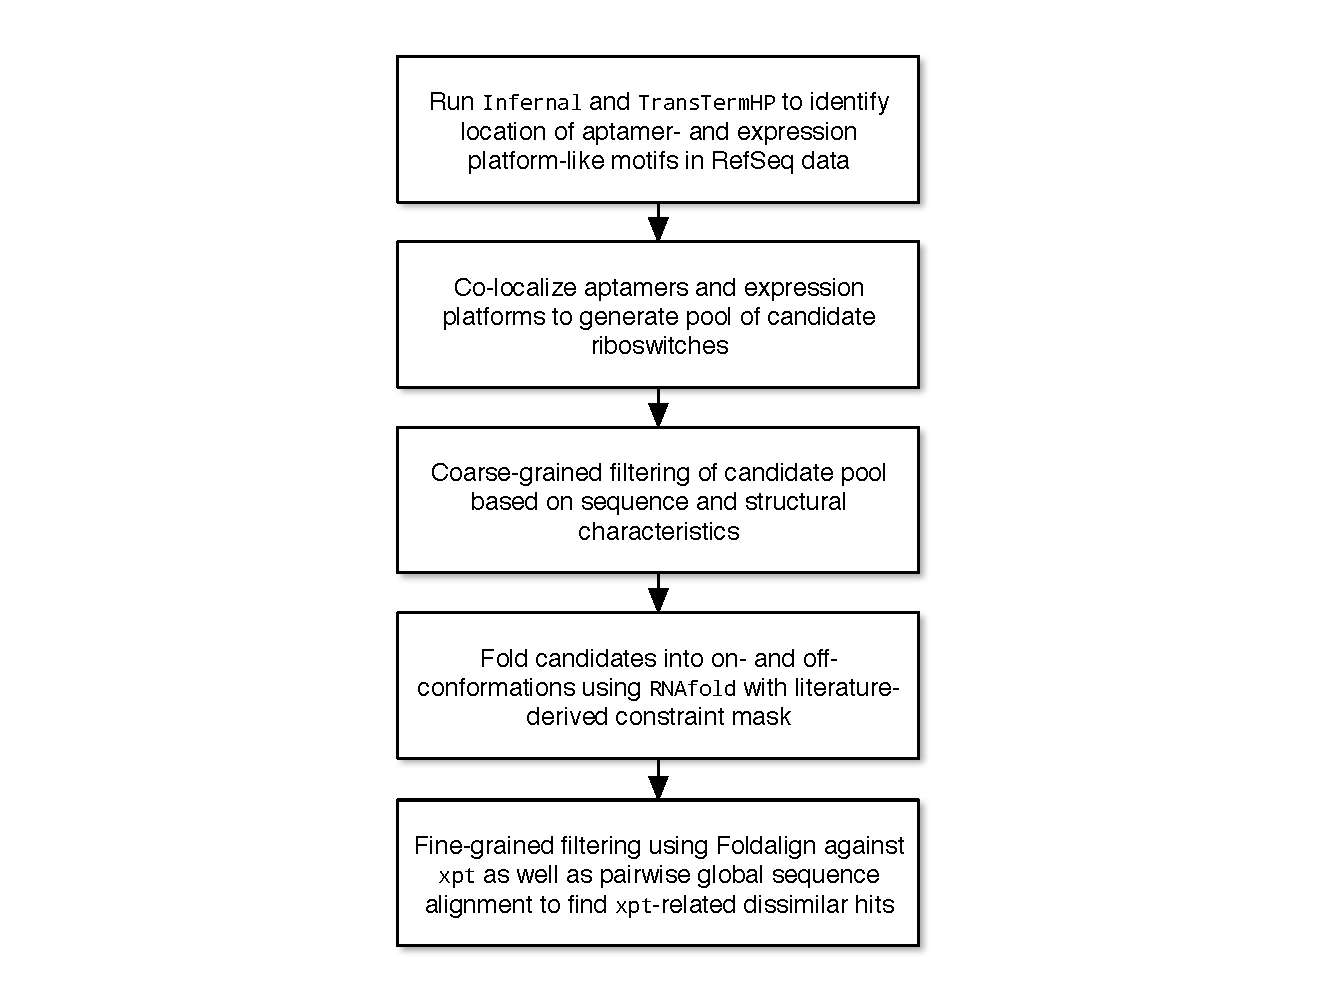
\includegraphics[width=.9\textwidth]{Figures/Ribofinder/ribofinderOverview.pdf}
\caption{Outline of the approach for the \rfinder pipeline.}
\label{fig:rfinder:flowchart}
\end{figure}

In the following discussion, we describe the application of \rfinder to identify
unannotated guanine purine \rbs; guanine-sensing cis-regulatory elements
which modulate the expression of genes involved in purine biosynthesis.

\subsection{Step 1: Candidate selection}
\label{subsec:rfinder:selection}

The RefSeq data we used for analysis contains 5,121 annotated bacterial genomes
across 2,732 different organisms, totaling over $9.5 * 10^9$ bases. We used the
program \infernal to determine the coordinates of putative aptamer structures
within the RefSeq genomes, and \tthp to locate candidate rho-independent
transcription terminators.

\subsubsection{Detecting Aptamers with \infernal}
\label{subsubsec:rfinder:infernal}

\infernal \citep{infernal}, \citep{nawrocki:2013hk} uses a stochastic context-free
grammar (SCFG) with a user-provided multiple sequence alignment (MSA) to
efficiently scan genomic data for RNA homologs, taking into consideration both
sequence and structural conservation. Using the purine aptamer MSA from RFam 12.0
(RF00167), \infernal (v1.1.1, default options) detects 1,537 significant hits
having E-value $<= 0.01$. Because \infernal leverages the concept of a
`local end'---a large insertion or deletion in the alignment at reduced cost---it
is possible for the software to return a significant hit whose aligned structure
does not have the canonical three-way junction observed in all purine
\rbs. \rfinder prunes these truncated \infernal hits by converting the
alignment structure into a parse tree, and only permitting trees of sufficient
complexity to contain a multiloop (described further in
\ref{subsubsec:rfinder:shapes}). The pyrimidine residue abutted next to the P1
stem in the J3--1 junction differentiates between guanine and adenine-sensing
\rbs by binding the complimentary purine ligand; for our interest in \grbs
exclusively we require the presence of a cytidine at this residue. In total, using
\infernal with these additional filters yields 1,280 guanine aptamers across 555
unique organisms (note: here and elsewhere I define a `unique organism' as having
a unique taxonomy ID).

\subsubsection{Detecting Expression Platforms with \tthp}
\label{subsubsec:rfinder:tthp}

\tthp \citep{ermolaeva:2000cl} detects rho-independent terminators in bacterial
genomes in a context-sensitive fashion by leveraging the protein annotations
available in PTT data. These terminator sequences canonically have a stable
hairpin loop structure immediately preceding a run of $5+$ uracil residues, the
combination of which causes the ribosomal machinery to stall and dissociate from
the transcript. \tthp performs a genomic scan to determine candidate loci with
this motif, and returns scored hits. The scoring system considers both structural
homology and the genomic contextual information available in the PTT file. Across
our collection of bacterial genomes acquired from NCBI RefSeq data, \tthp
identified 2,752,469 rho-independent terminators using the default filters.

Due to the spatially-mediated structural regulation of purine \rbs,
whereby ligand interaction with the aptamer domain induces local structural
rearrangement in the expression platform, we paired aptamers with corresponding
terminators by minimizing the genomic distance, with an upper bound of 200
nucleotides between the end of the aptamer domain and start of the terminator.
This approach yields 577 candidate \rbs, 81 of which have multiple
rho-independent terminators within range of a putative aptamer produced by
\infernal. For these, we simply pair the closest \tthp hit with the aptamer domain.

\begin{figure}[!ht]
\centering
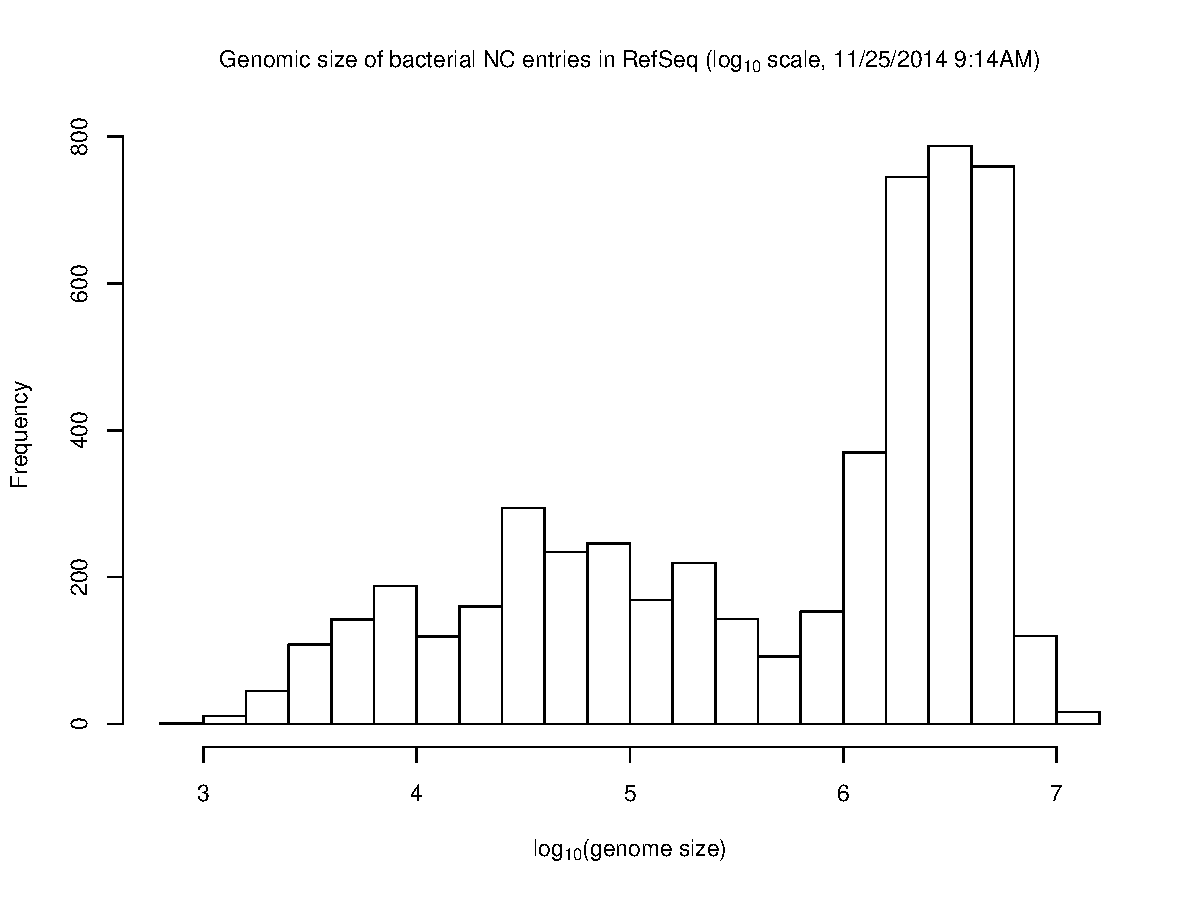
\includegraphics[width=.9\textwidth]{Figures/Ribofinder/refseqGenomeSizes.pdf}
\caption{Histogram displaying the distribution of genome sizes across the RefSeq
data analyzed, comprising 5,172 bacterial genomes. Genome size is shown using a
$\log_{10}$ scale.}
\label{fig:rfinder:genomeSizes}
\end{figure}

\subsection{Step 2: Structural prediction}
\label{subsec:rfinder:strpred}

Until this point we have been focused on the generation of candidate sequences
from our RefSeq dataset, without yet focusing on the specifics of underlying
secondary structures for these candidates. In the following section, we explain
how constraint folding is used to generate putative `on' and `off' conformations
for each candidate.

\subsubsection{Notation for Representing Abstract RNA Shapes}
\label{subsubsec:rfinder:shapes}

Given an RNA sequence $\seq = \seqN$, where positions $s_i$ are drawn from the
collection of single-letter nucleotide codes, i.e.
$s_i \in \{\text{A,\,U,\,G,\,C}\}$, it is possible to describe a corresponding
secondary structure \strS compatible with \seq using the dot-bracket notation.
In this notation, each nucleotide $a_i$ has a corresponding state $s_i$, where
$s_i$ is denoted as a `.' if unpaired and a `(' [resp. `)'] if the left [resp.
right] base in a base pair. Given any two base pairs $(i,j)$ and $(k,l)$ in \strS,
then $i < k < j \iff i < l < j$; pseudoknots are not permitted in the structure. A
secondary structure taking this form is said to have balanced parentheses, and can
additionally be represented using a context-free grammar such as:

\begin{align}
\label{eq:rfinder:strCfg}
S \rightarrow S\,.\;|\;.\,S\;|\;(S)\;|\;SS\;|\;\epsilon
\end{align}

The grammar from \eqnref{rfinder:strCfg} can be used to generate a parse tree
\tree for \strS. The benefit of working with \tree over \strS is that the parse
tree offers an abstract representation of secondary structure shape independent of
sequence length, permitting us to classify and eventually constrain a large
collection of sequences having variable length which are all expected to have the
same abstract tree shape. This is analogous to what the Giegerich lab refers to as
their `type 5' structural abstraction using the \rshapes tool. Every node in \tree
represents a helix in \strS, and internally tracks the indices of both its
beginning $(i,j)$ and closing $(k,l)$ base pair. We use a level-order naming
convention to refer to helices within the parse tree, whereby a position
\treePos{p}{1} references the first child of the root node, \treePos{p}{1,2}
references the second child of \textdown{\ms{p}}{1}, and generally
\treePos{p}{$i_1,i_2,\cdots,i_n$} refers to the $i_n$\textsuperscript{th} child of
\treePos{p}{$i_1,i_2,\cdots,i_{n-1}$}. To reference specific nucleotides in the
context of their location relative to a helix, we use the opening and closing base
pairs $(i,j)$ and $(k,l)$ as landmarks. Thus, \treeIdx{p}{1}{l} is the index in
\strS of the right-hand side closing base pair of \treePos{p}{1}. We use the
notation \treePos{t}{$i$} to refer to the subtree of \tree whose root is
\treePos{p}{$i$}.

Finally, we introduce the concept of a tree signature. The tree signature for a
tree \tree is a list of the node depths when traversed in a depth-first pre-order
fashion. To provide a concrete example, consider the following experimentally
validated xpt \grb from Bacillus subtilis subsp. subtilis str. 168
(NC\_000964.3 2320197--2320054) with corresponding gene off structure as seen in
\Figref{rfinder:xptOff}.
\medskip

\begin{figure}[!ht]
\centering
\begin{subfigure}[h]{\textwidth}
\centering
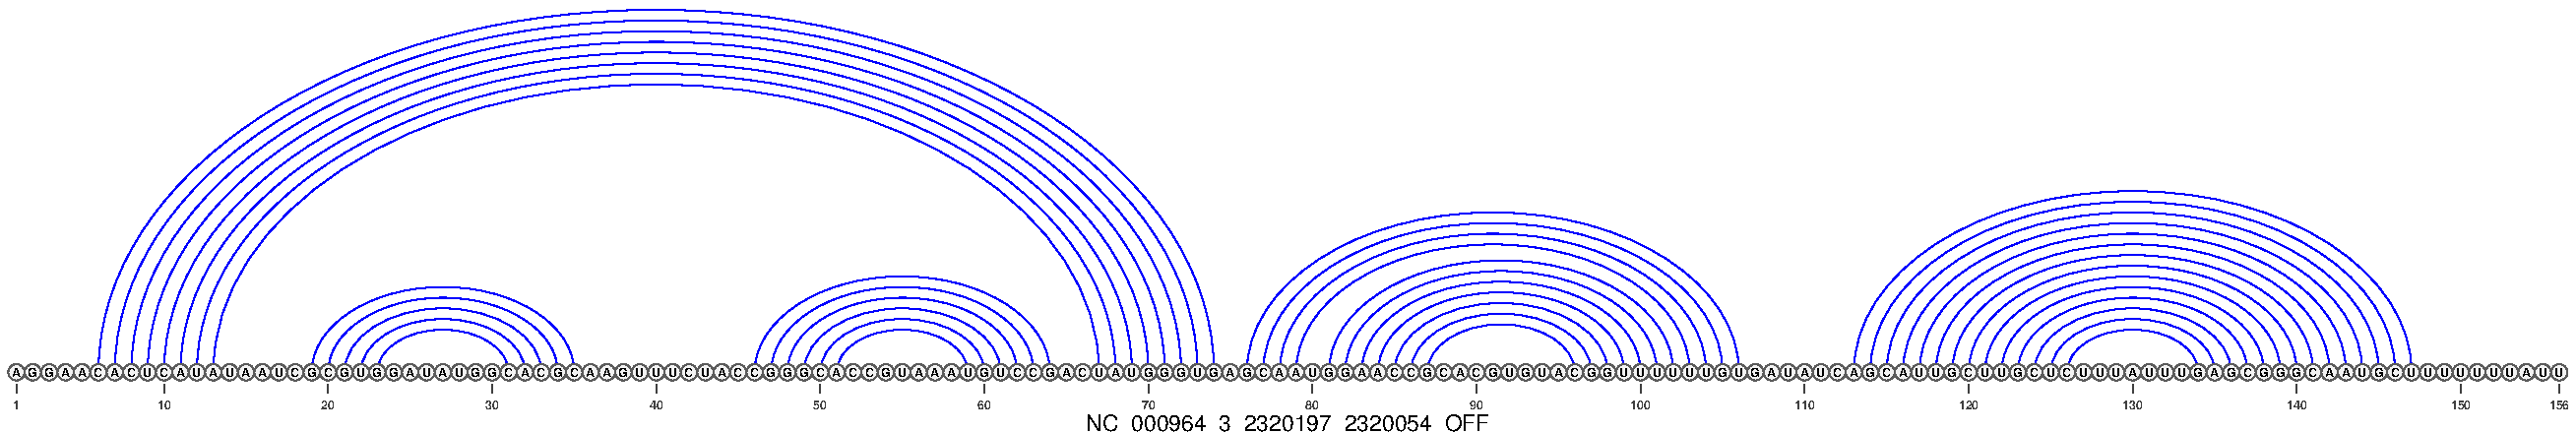
\includegraphics[width=.9\textwidth]{Figures/Ribofinder/NC_000964_3_2320197_2320054_OFF.pdf}
\end{subfigure} \\
\medskip
\begin{subfigure}[h]{\textwidth}
\centering
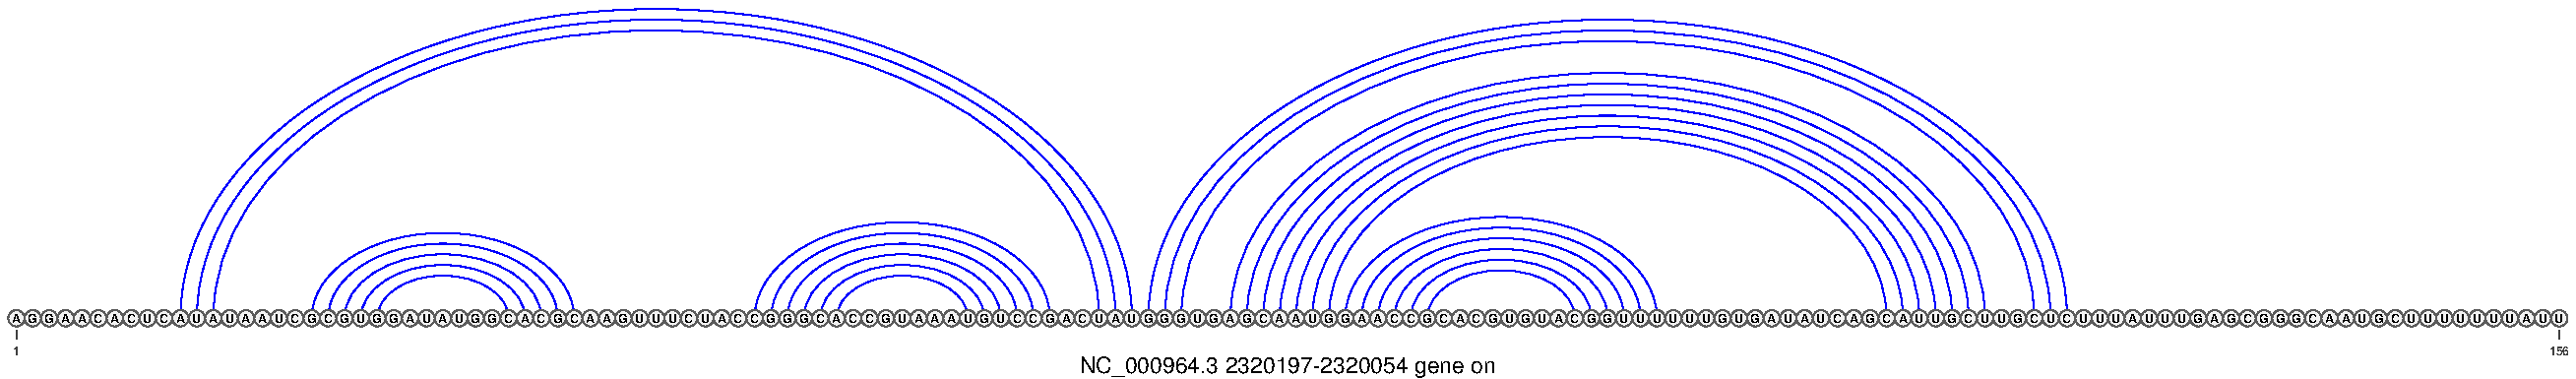
\includegraphics[width=.9\textwidth]{Figures/Ribofinder/NC_000964_3_2320197_2320054_ON.pdf}
\end{subfigure}
\caption{{\em (Top)} The xanthine phosphoribosyltransferase (xpt) \grb from
{\em B. subtilis} subsp. subtilis str. 168 (NC\_000964.3 2320197--2320054),
and corresponding gene off structure derived from crystallography analysis in
complex with guanine \citep{breaker:riboswitch2}. {\em (Bottom)} The experimentally
derived gene on structure for \Bsxpt. These structural diagrams were generated
using VARNA \citep{darty:2009gt}.}
\label{fig:rfinder:xptOff}
\end{figure}

The \rshapes \citep{janssen:2015cq} `type 5' representation for this structure is
\ms{[[][]][][]} (note the coalesced left bulge in the hairpin immediately
downstream the closing multiloop stem, at helix \treePos{p}{2}) and the tree
signature for this parse tree of the structure is \ms{[0,1,2,2,1,1]}.

We leverage the notion of abstract structural filtering initially to ensure that
all \infernal aptamer hits have a tree signature of \ms{[0,1,2,2]}, which
represents a three-way junction, and that the binding site for the guanine ligand
$\treeIdx{p}{1}{l - 1} = \text{C}$. These filters, in combination with the
proximal terminator hairpins produced by \tthp yield the aforementioned 577
candidate \grbs for which we then try to produce reasonable gene on and off
structures.

\subsubsection{Constrained Folding to Predict Switch Structures}
\label{subsubsec:rfinder:consfold}

To restrict our search to unannotated \grbs, and further ensure that we are not
re-detecting sequences based off the RFam covariance model provided to \infernal,
we constrain our search to those RefSeq organisms not represented in the RFam seed
alignment. 503 of the 577 candidates, or 87.18\% represent putative unannotated
\rbs not represented by RF00167.

The gene off structure \strOff for a \grb is the easier of the two to find
computationally, since the terminator stem is exceptionally thermodynamically
stable. In the gene on conformation \strOn, the P1 stem of the multiloop partially
dissociates and an anti-terminator stem forms between the region immediately 3' of
the P1 stem and what was the left-hand side of the terminator stem. This truncated
P1 stem, which closes the three-way junction in the aptamer, is exceptionally
unstable based on present energy models available for structural folding, and
requires special treatment to reconstitute in our final structures.

The software \rfold (v2.1.8) allows for the folding of RNA molecules with `loose'
constraints. In this model of constrained folding, the resulting structure
produced by the software guarantees not to explicitly invalidate any user-provided
constraints, but does not guarantee all constraints will be satisfied in the
resulting structure. For each of the candidate \grbs, having \treeFor{\infernal}
and \treeFor{\tthp}, we build the following constraint masks:

{\large Structural constraints for both conformations of the \grb aptamer:}
\begin{enumerate}
\setstretch{1.3}
\item Prohibit base pairing upstream of \treeIdx{p}{1}{i} and
downstream of \treeIdx{p}{2}{l}. \\[1.5ex] {\em Do not permit any possible disruptive pairing
interactions 5' of the aptamer or 3' of the terminator stem.}
\item Force base pairs and unpaired regions in \treePos{t}{1}, with
the exception of \treePos{p}{1}. \\[1.5ex] {\em Since the aptamer structure is well
conserved and we have the \infernal-provided alignment with the
covariance model, force this structure to form as aligned.}
\item Explicitly prohibit formation of \treePos{p}{1} stem, which closes the
three-way junction. \\[1.5ex] {\em The only exception to above is the closing of the
P1 multiloop stem. In our experience, since \rfold uses soft constraints
(meaning that constrained base pairs are only allowed to pair with each other
or not at all), in practice we rarely see the P1 stem form as we would like.
Instead, restrict it from forming at all, so that it can be added in after the
fact without disrupting any other base pairs.}
\end{enumerate}
{\large Constraints exclusive to the gene off structure:}
\begin{enumerate}
\setstretch{1.3}
\item Force base pairs and unpaired regions in \treePos{t}{2}. \\[1.5ex] {\em This simply
forces the formation of the terminator stem, as predicted by \tthp.}
\end{enumerate}
{\large Constraints exclusive to the gene on structure:}
\begin{enumerate}
\setstretch{1.3}
\item Require $m$ nucleotides starting from \treeIdx{p}{1}{l + 3} to pair to the
right, where $m = \textit{length}(\treePos{p}{2})$, and require the left-hand side of the
\treePos{p}{2} helix to pair to the left. \\[1.5ex] {\em The formation of the
anti-terminator stem involves the partial disruption of the \treePos{p}{1} stem.
Though there is no consensus for the length of the anti-terminator stem,
experimental data suggests that the left side of the terminator stem}
(\treeIdx{p}{2}{i}--\treeIdx{p}{2}{k}) {\em alternatively base pairs to the left,
thus forming the anti-terminator hairpin and permitting transcription to proceed
\citep{mandal:2004ja}.}
\item Disallow pairing downstream of \treeIdx{p}{2}{j}. \\[1.5ex] {\em Avoid
disruptive pairing downstream of the newly formed anti-terminator stem.}
\end{enumerate}

These constraint masks are run using the command-line flags
\ms{-d 0 -P rna\_turner1999.par} to disable dangles and use the Turner 1999
energies respectively. Experimental evidence using inline probing and
crystallographic analysis suggests that
the `on' conformation of the \grb has a reduced P1 stem length of 3 base pairs
\citep{mandalboesebarrickwinklerbreaker,serganov:2004dq};
in practice we were unable to force \rfold to respect this constraint regardless
of command-line options specified. For this reason we reconstitute the P1 stem in
both structures after constrained folding, having length equivalent to it the
\infernal P1 stem (resp. 3 base pairs) in the gene off (resp. gene on) structure.

This difficulty with \rfold can be shown by using the constraint-produced
structures as exhaustive constraints themselves. All unpaired nucleotides in
\strOff and \strOn are notated by a `\ms{x}' and all base pairs by `\ms{()}' for
the 5' and 3' side of the pair respectively to form new constraints mask
\strConst{off} and \strConst{on}, having all bases' state explicitly specified. By
refolding all 577 candidate sequences with \strConst{off} and \strConst{on} using
the same options as before, only 463 (or 80.24\%) of the resulting structures from
\strConst{off} have the tree signature prefix \ms{[0,1,2,2,1]}, and just 21 (or
3.64\%) of the \strConst{on} structures correctly re-fold their multiloop.

\subsection{Step 3: Candidate curation}
\label{subsec:rfinder:curation}

Until now, we have described our approach for generating the 503 \grb candidates
in RefSeq, alongside their gene on and off structures. Unfortunately the
experimental validation of all 503 candidates is not tractable, so it was
necessary to reduce this collection again to a more manageable size, while only
keeping the most promising candidates. Our original approach involved using
\foldalign \citep{havgaard:2007ca} alongside the \ms{needleall} tool from EMBOSS
\citep{rice:2000wr}, to simultaneously
select sequences which closely approximate the more thermodynamically stable
gene off conformation of the experimentally known \Bsxpt \grb, while minimizing
sequence similarity between candidates selected for experimental validation. Due to
experimental constraints, we elected finally to instead choose a small number
($n = 2$) of organisms easily available which had multiple promising hits as our
experimental candidate pool.

In \Figref{rfinder:histogramFoldalignCandidatesVsXpt}, we display a histogram of scores produced
by \foldalign for the 503 candidates, when aligned with the \Bsxpt \grb. \foldalign
is based off Sankoff's algorithm \citep{sankoff:1985wc}, a dynamic programming
algorithm for simultaneous folding and alignment that runs in \On{6} time and
\On{4} space. Because three of the sequences from our pool of 503 candidates have
no global alignment with the \Bsxpt sequence, we have pruned them from our
dataset and only consider those remaining 500 sequences for which \foldalign
scores are produced. The \foldalign scores produce have a mean of $153.798$ with a
minimum [resp. maximum] score of $-2698$ [resp. 1908]. Running \foldalign with the
\Bsxpt sequence aligned with itself produces a theoretical maximum score of 2419.

\begin{figure}[!ht]
\centering
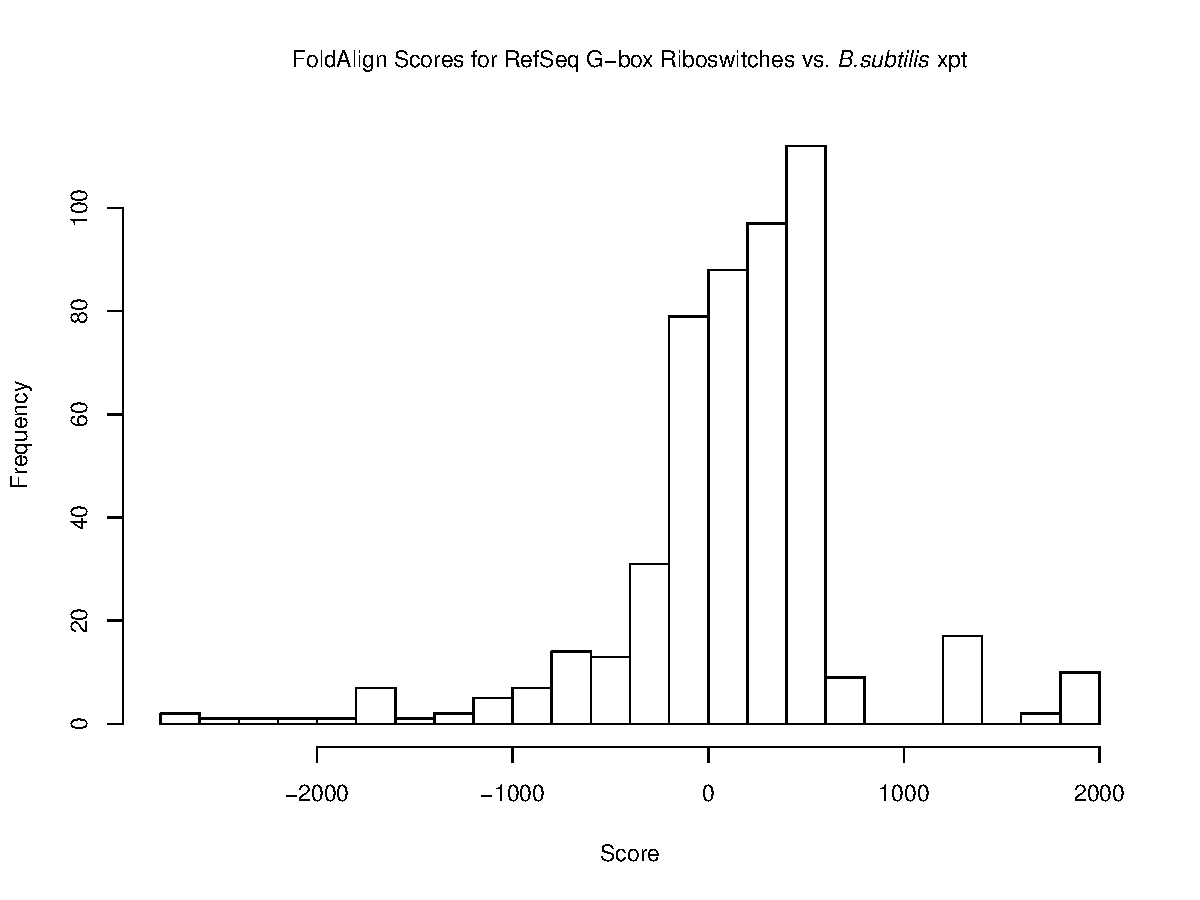
\includegraphics[width=.9\textwidth]{Figures/Ribofinder/histogramFoldalignCandidatesVsXpt.pdf}
\caption{Histogram displaying the distribution of scores produced by \foldalign
2.1.1 using flags \ms{-global -summary -format commandline} when folding each of
the 503 candidates against the \Bsxpt sequence NC\_000964.3 2320197--2320054.
Three of the sequences run against \foldalign (NC\_010674.1 1516712--1516868,
NC\_010723.1 1487041--1487197, and NC\_020291.1 4599412--4599258) have no global
alignment with the \Bsxpt sequence, and thus the histogram represents 500 of the
original 503 sequences.}
\label{fig:rfinder:histogramFoldalignCandidatesVsXpt}
\end{figure}

Of these 500 sequences, 335 have a \foldalign score $s > 0$, representing 227
unique accession numbers, with a distribution of candidates per accession number
as shown in \Figref{rfinder:candidateHistogramGroupedByAccession}. From
the perspective of experimental validation, we have tried to maximize the chance
of success per organism by selecting those having multiple candidates within the
same genome. Only 25 of the candidate organisms have more than three hits within
their genome (only two have five hits). Our approach for selecting the initial
two organisms for experimental validation was to take this pool of 25 organisms,
sort by descending average score $s$, and select the first two which are available
via DSMZ (\url{https://www.dsmz.de/}), the warehouse for microorganisms used by
our collaborators. Prof. Dr. Mario M\"orl at Universit\"at Leipzig is presently
overseeing a post-doc who is using the SHAPE protocol \citep{wilkinson:2006vd} to
validate the computationally predicted structure of these candidates.

\begin{figure}[!ht]
\centering
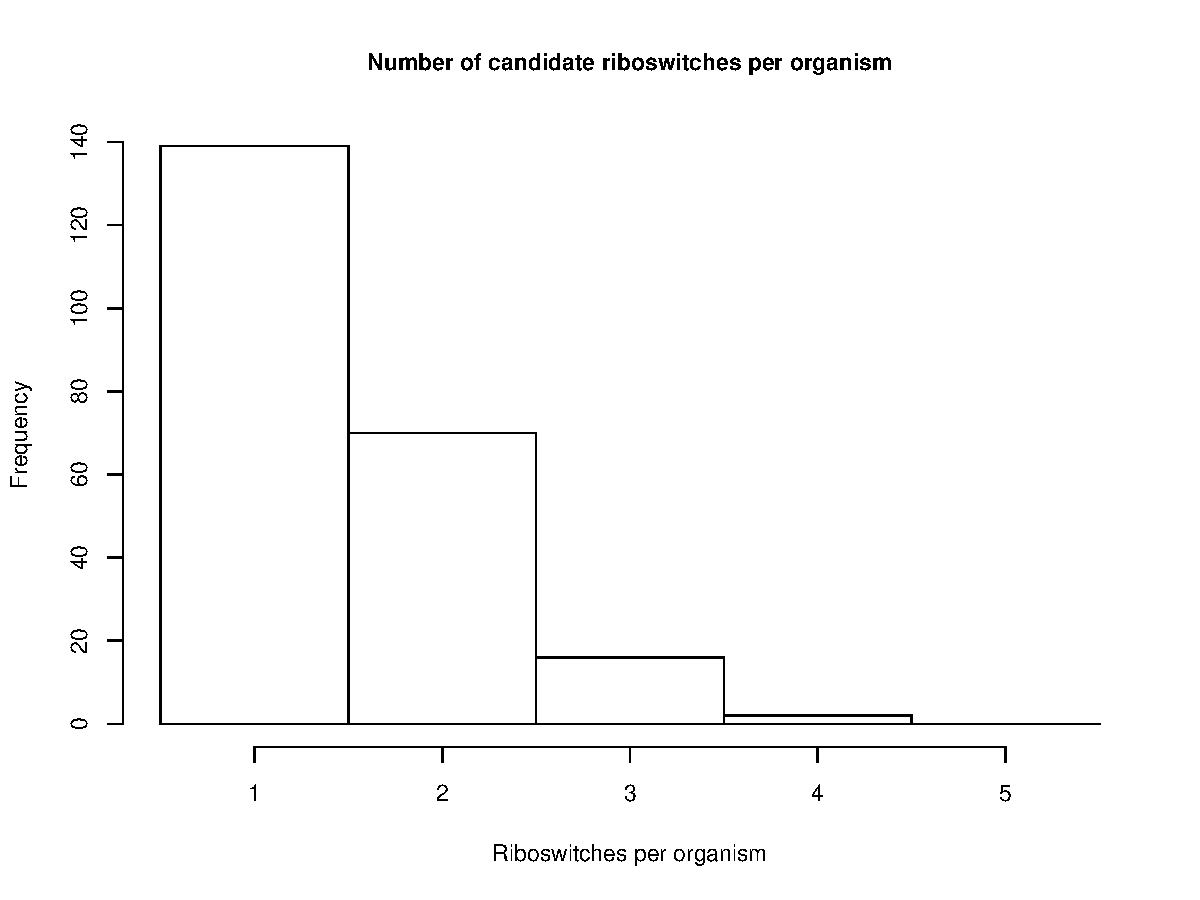
\includegraphics[width=.9\textwidth]{Figures/Ribofinder/candidateHistogramGroupedByAccession.pdf}
\caption{Histogram displaying the distribution of scores produced by \foldalign
2.1.1 using flags \ms{-global -summary -format commandline} when folding each of
the 503 candidates against the \Bsxpt sequence NC\_000964.3 2320197--2320054.
Three of the sequences run against \foldalign (NC\_010674.1 1516712--1516868,
NC\_010723.1 1487041--1487197, and NC\_020291.1 4599412--4599258) have no global
alignment with the \Bsxpt sequence, and thus the histogram represents 500 of the
original 503 sequences.}
\label{fig:rfinder:candidateHistogramGroupedByAccession}
\end{figure}

Proceeding in this fashion, we have selected {\em B. megaterium} QM B1551
(\href{http://www.ncbi.nlm.nih.gov/nuccore/NC_014019.1}{NC\_014019.1},
\href{http://www.dsmz.de/catalogues/details/culture/DSM-1804.html}{DSM1804})
and {\em B. megaterium} DSM319
(\href{http://www.ncbi.nlm.nih.gov/nuccore/NC_014103.1}{NC\_014103.1},
\href{http://www.dsmz.de/catalogues/details/culture/DSM-319.html}{DSM319})
for initial validation. These organisms have four
candidate \grbs each, outlined in Table \ref{table:rfinderCandidateLocs}.

\begin{table}[!ht]
\centering
\begin{tabularx}{\linewidth}{*{1}{L} *{2}{C}}
  \toprule
  \small{Downstream gene function} & \small{{\em B. megaterium} QM B1551} & \small{{\em B. megaterium} DSM319} \\
  \cmidrule(lr){1-3}
  \small{xpt} & 1427313--1427501 & 1413696--1413884 \\[1ex]
  \small{GMP synthase} & 231630--231806 & 230059--230235 \\[1ex]
  \small{guanine permease} & 233482--233680 & 231911--232108 \\[1ex]
  \small{N5-carboxyaminoimidazole} & 240759--240970 & 239188--239400 \\
  \bottomrule
\end{tabularx}
\caption{The genomic coordinates for the four candidate \grbs in both
{\em B. megaterium} QM B1551 and {\em B. megaterium} DSM319. Note that the
\grbs are located upstream of the same genes, and that these two strains of
{\em B. megaterium} are highly similar. These structures are pictured in
\Secref{sec:rfinder:grbValidationVarna}, plotted using VARNA
\citep{darty:2009gt}.}
\label{table:rfinderCandidateLocs}
\end{table}

\section{Extending beyond \grbs}
\label{sec:rfinder:ext}

We believe that the \rfinder pipeline allows for the detection of both structural
conformations of \rbs beyond the \grb. The investigation of
adenine-sensitive purine \rbs is a small extension of the existing
implementation. As indicated in \Secref{subsubsec:rfinder:infernal}, adenine
\rbs have a complimentary uradine residue at the ligand binding site in
the J3--1 junction within the aptamer. Beyond differences in ligand specificity,
the adenine \rb anti-terminator stem is incorporated into the aptamer structure
itself, and thus stabilized with the base pairing of the adenine ligand. As a
result, the adenine riboswitch permits transcription when bound, unlike the \grb.
As a result of the extensive overlap between the anti-terminator stem and adenine
\rb aptamer, the formation of the terminator stem completely dissociates both the
P3 and P1 stems \citep{mandal2004a}.

From a computational perspective, these changes are simple to handle within the
\rfinder pipeline, and provide some indication to how we believe the framework
could be more generally applied in the future. Rather than filter for the
discriminatory cytidine residue in the \rb aptamer (\Secref{subsubsec:rfinder:infernal}) we can only select those hits from \infernal having a uridine at the
ligand binding site. Structural on and off conformations are known from
experimental data for the {\em B. subtilis} ydhL gene \citep{mandal2004a} and can
be used as templates for the constraint masks used in \Secref{subsec:rfinder:strpred}.

In general, we believe those riboswitches using rho-independent transcription
termination as a mode of regulation, for which an aptamer alignment exists and
some experimental knowledge of the terminator stem's structural conformation are
well suited for more robust structural prediction using \rfinder.

\section{Guanine \rbs for experimental validation}
\label{sec:rfinder:grbValidationVarna}

\begin{figure}[!ht]
\centering
\begin{subfigure}[h]{\textwidth}
\centering
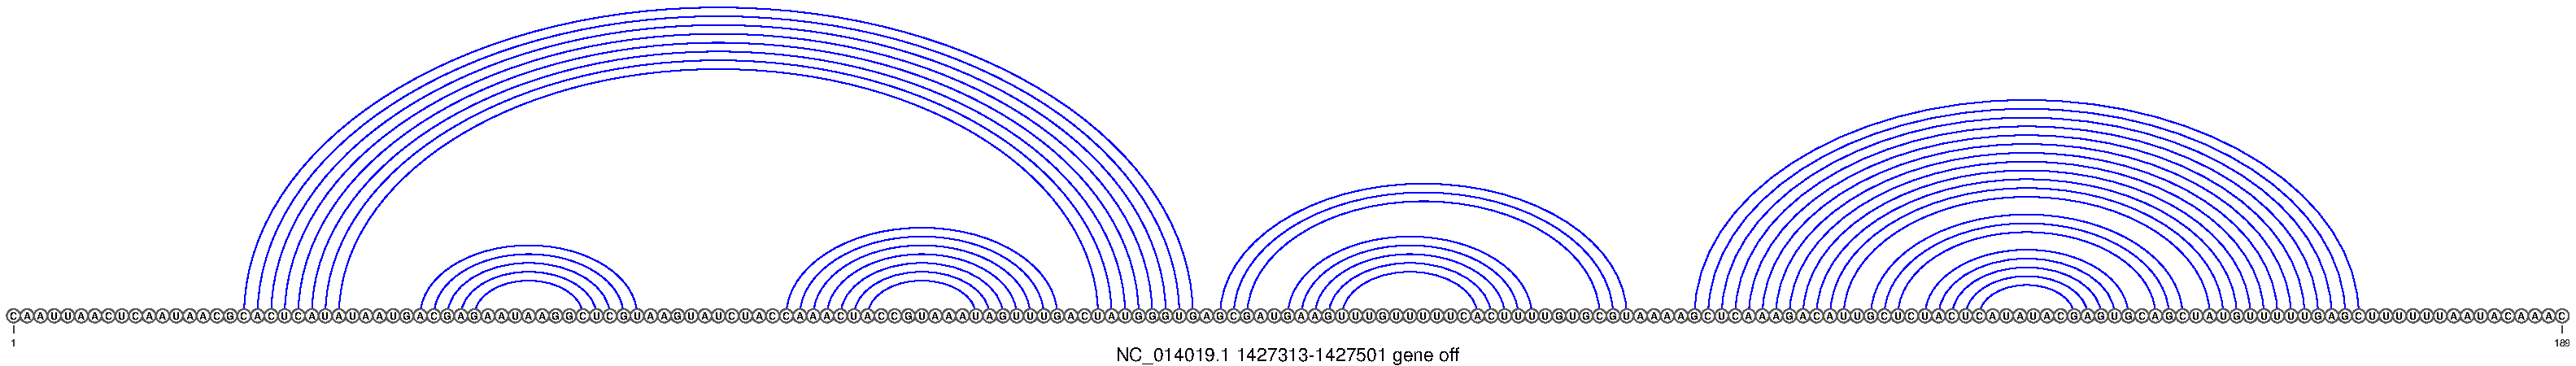
\includegraphics[width=.9\textwidth]{Figures/Ribofinder/NC_014019_1_1427313_1427501_OFF.pdf}
\end{subfigure} \\
\medskip
\begin{subfigure}[h]{\textwidth}
\centering
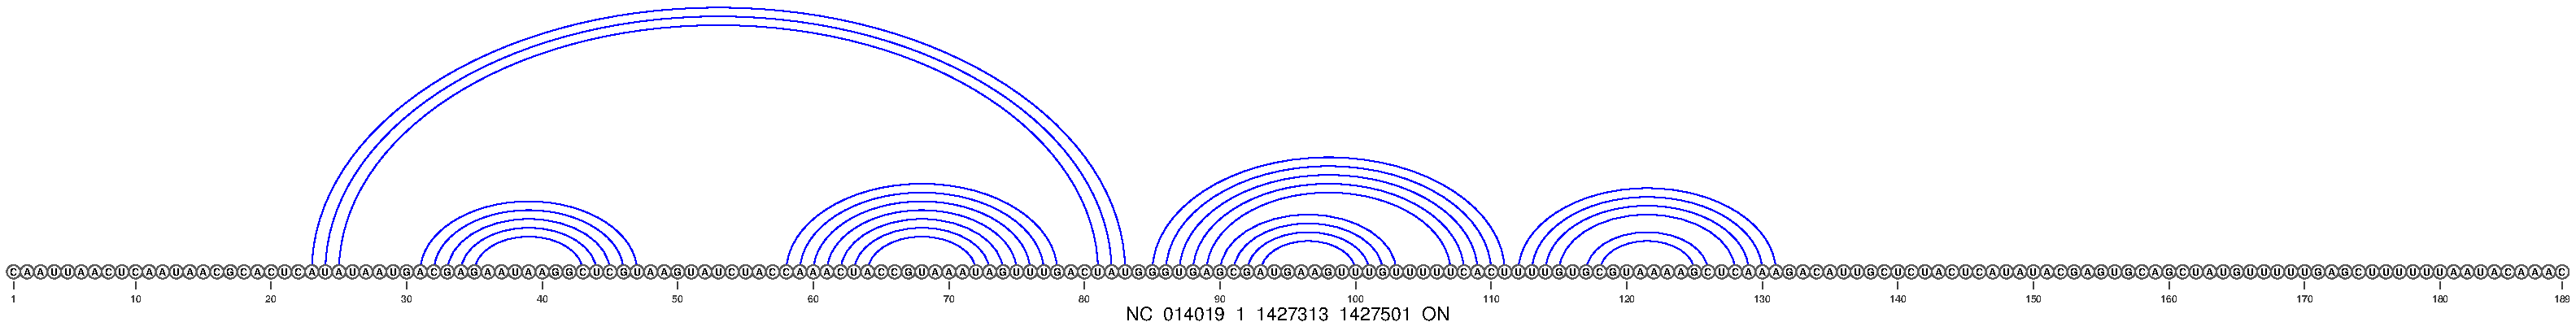
\includegraphics[width=.9\textwidth]{Figures/Ribofinder/NC_014019_1_1427313_1427501_ON.pdf}
\end{subfigure}
\caption{{\em Top:} the computationally predicted gene off conformation of
sequence NC\_014019.1 1427313--1427501, using \rfold from the ViennaRNA 2.1.8
suite, with dangles disabled and the Turner 1999 energies. This sequence is
located upstream of the xpt gene in {\em B. megaterium} QM B1551. {\em Bottom:}
the gene on conformation.}
\label{fig:figure:NC_014019_1_1427313_1427501}
\end{figure}
\medskip

\begin{figure}[!ht]
\centering
\begin{subfigure}[h]{\textwidth}
\centering
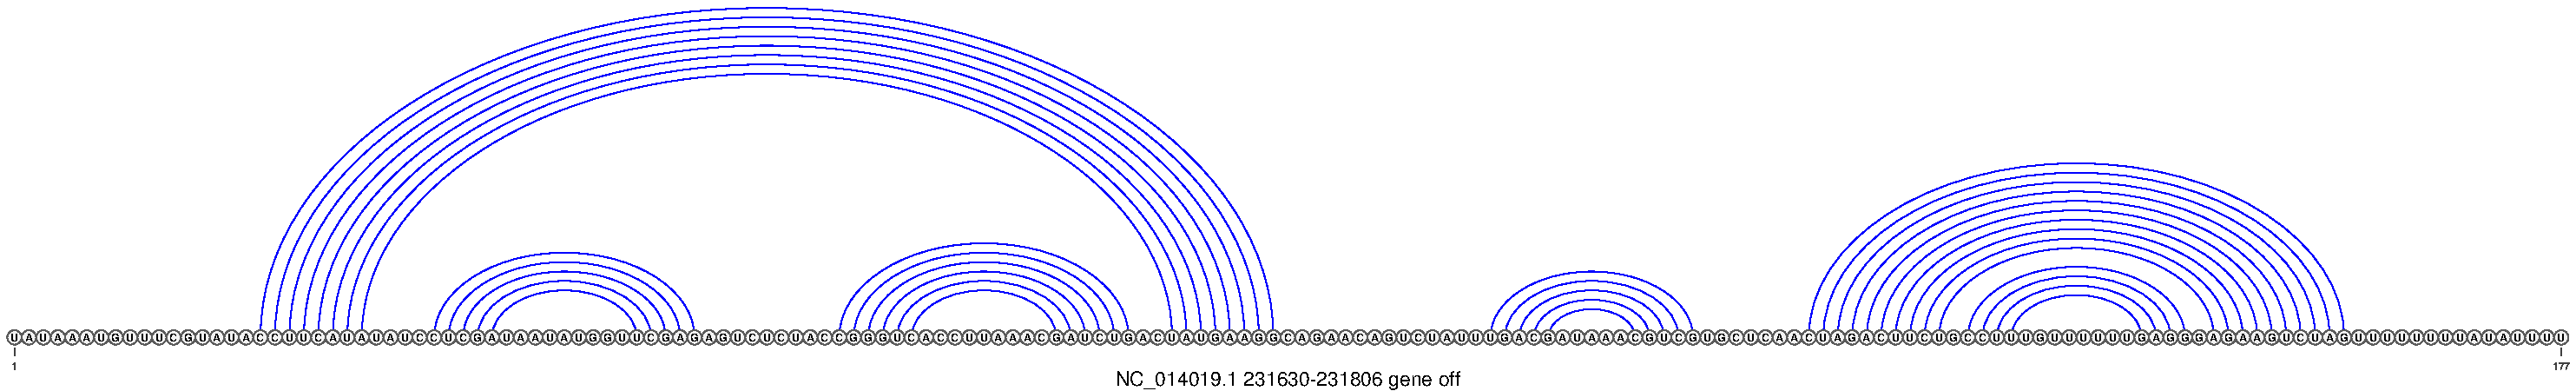
\includegraphics[width=.9\textwidth]{Figures/Ribofinder/NC_014019_1_231630_231806_OFF.pdf}
\end{subfigure} \\
\medskip
\begin{subfigure}[h]{\textwidth}
\centering
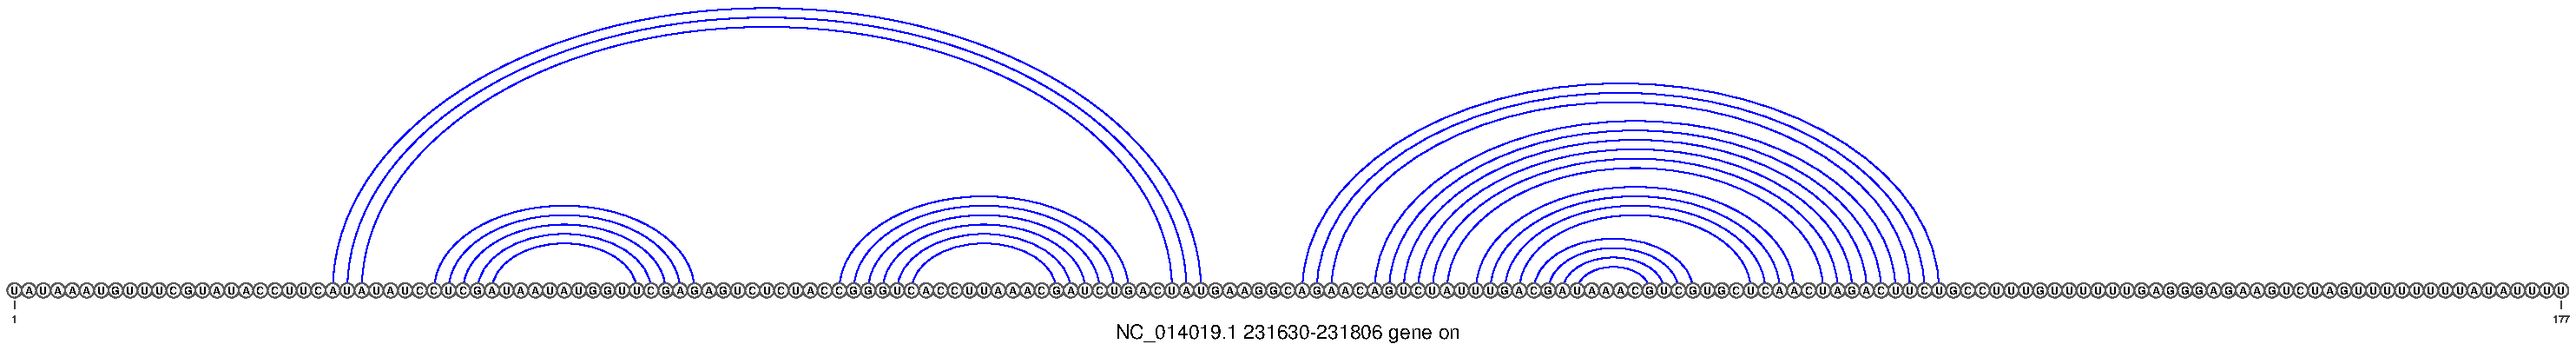
\includegraphics[width=.9\textwidth]{Figures/Ribofinder/NC_014019_1_231630_231806_ON.pdf}
\end{subfigure}
\caption{The computationally predicted \rb located upstream of the GMP synthase
gene in {\em B. megaterium} QM B1551 (NC\_014019.1 231630--231806).
{\em Top:} The gene off conformation. {\em Bottom:} The gene on conformation.}
\label{fig:figure:NC_014019_1_231630_231806}
\end{figure}
\medskip

\begin{figure}[!ht]
\centering
\begin{subfigure}[h]{\textwidth}
\centering
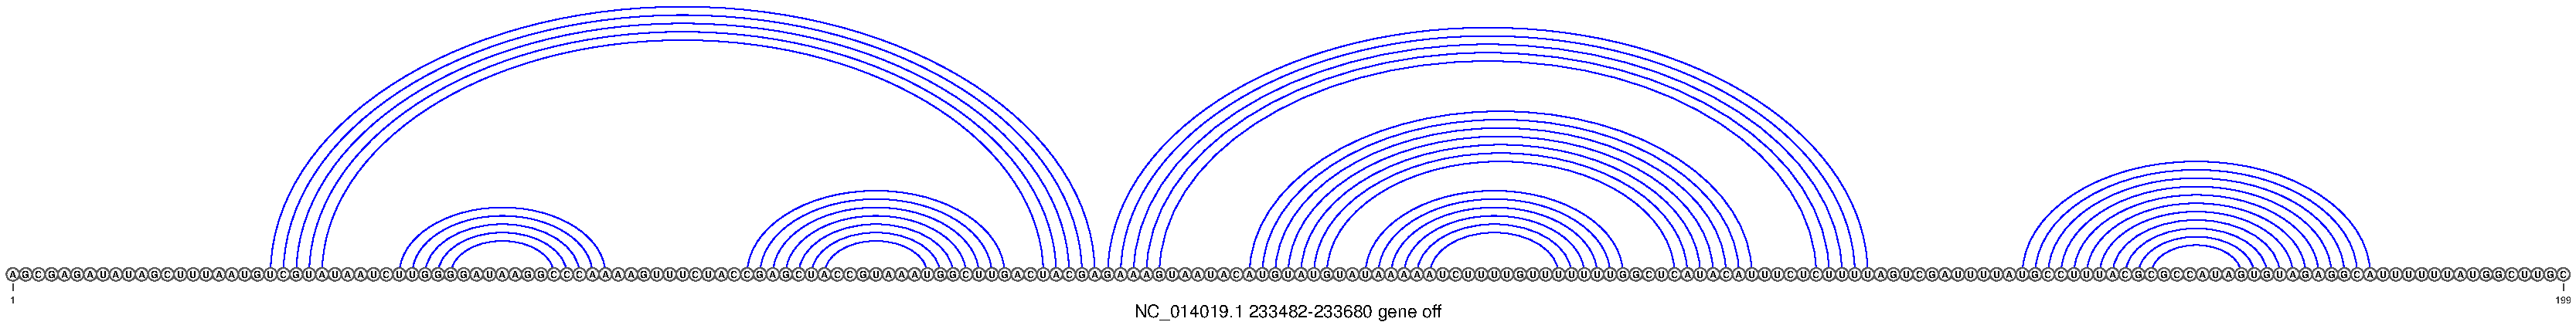
\includegraphics[width=.9\textwidth]{Figures/Ribofinder/NC_014019_1_233482_233680_OFF.pdf}
\end{subfigure} \\
\medskip
\begin{subfigure}[h]{\textwidth}
\centering
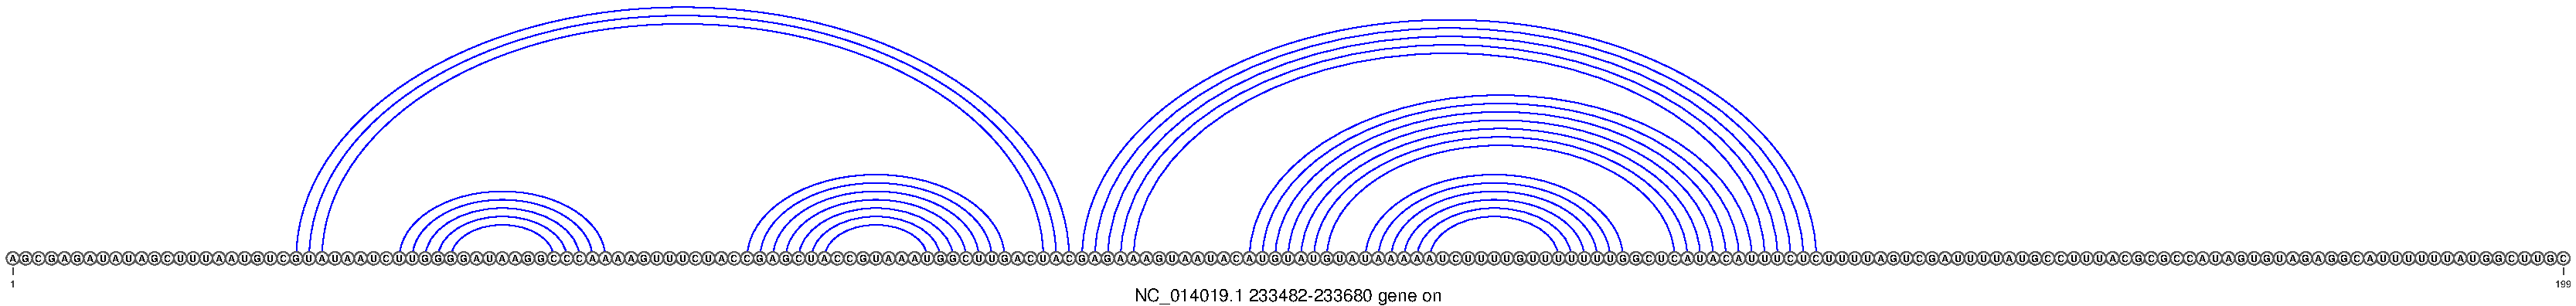
\includegraphics[width=.9\textwidth]{Figures/Ribofinder/NC_014019_1_233482_233680_ON.pdf}
\end{subfigure}
\caption{The computationally predicted \rb located upstream of the guanine permease
gene in {\em B. megaterium} QM B1551 (NC\_014019.1 233482--233680).
{\em Top:} The gene off conformation. {\em Bottom:} The gene on conformation.}
\label{fig:figure:NC_014019_1_233482_233680}
\end{figure}
\medskip

\begin{figure}[!ht]
\centering
\begin{subfigure}[h]{\textwidth}
\centering
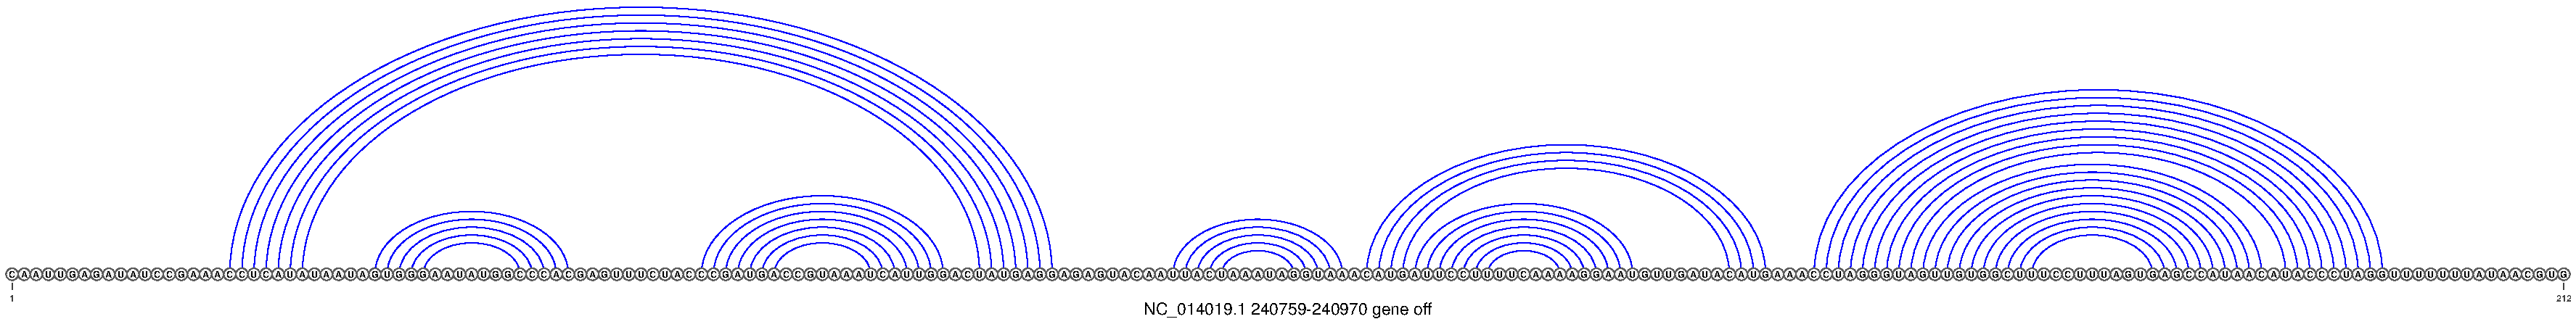
\includegraphics[width=.9\textwidth]{Figures/Ribofinder/NC_014019_1_240759_240970_OFF.pdf}
\end{subfigure} \\
\medskip
\begin{subfigure}[h]{\textwidth}
\centering
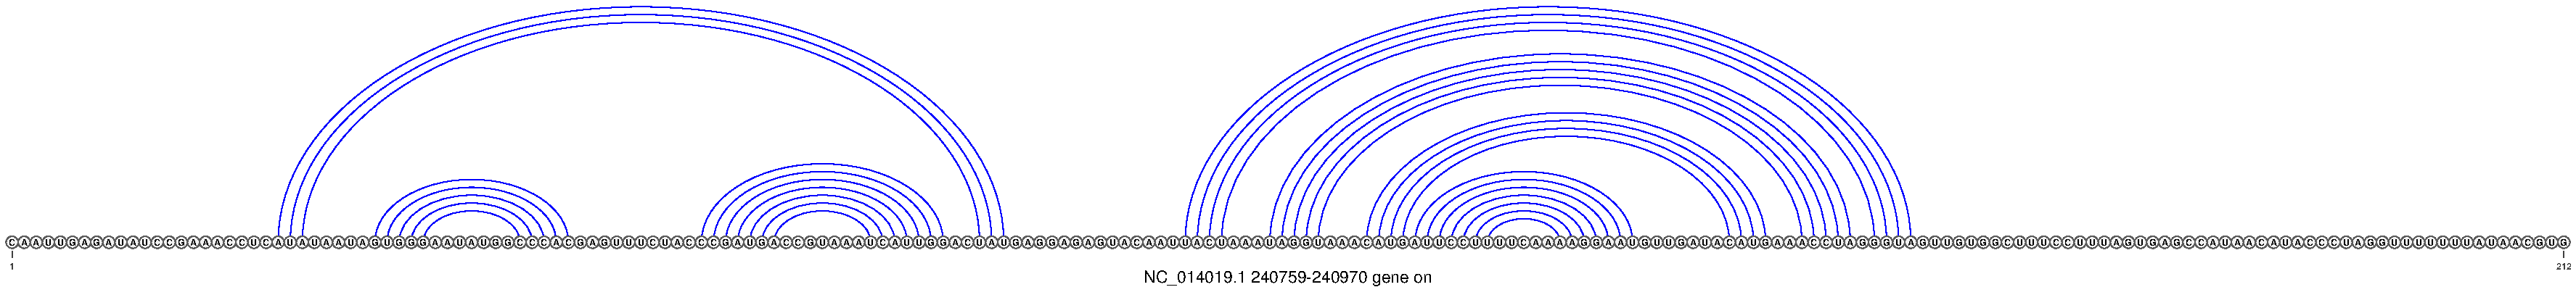
\includegraphics[width=.9\textwidth]{Figures/Ribofinder/NC_014019_1_240759_240970_ON.pdf}
\end{subfigure}
\caption{The computationally predicted \rb located upstream of the
N5-carboxyaminoimidazole
gene in {\em B. megaterium} QM B1551 (NC\_014019.1 240759--240970).
{\em Top:} The gene off conformation. {\em Bottom:} The gene on conformation.}
\label{fig:figure:NC_014019_1_240759_240970}
\end{figure}
\medskip

\begin{figure}[!ht]
\centering
\begin{subfigure}[h]{\textwidth}
\centering
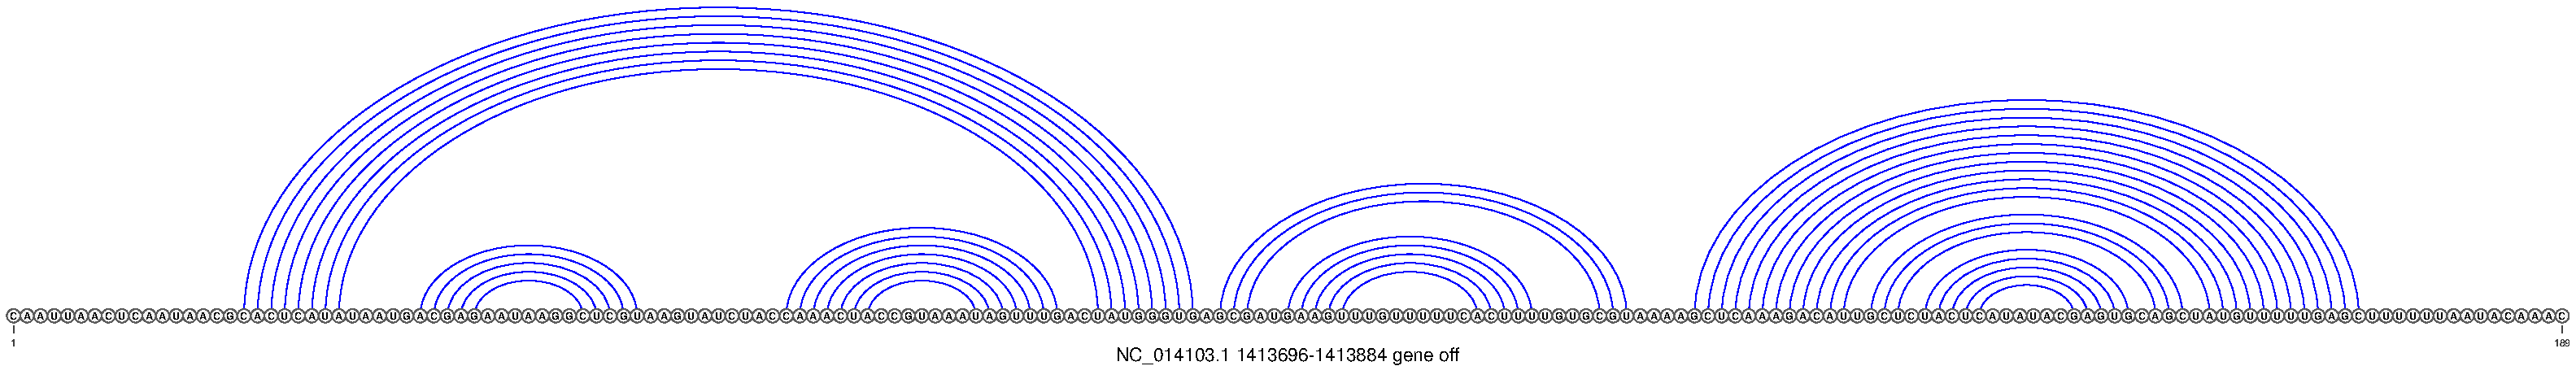
\includegraphics[width=.9\textwidth]{Figures/Ribofinder/NC_014103_1_1413696_1413884_OFF.pdf}
\end{subfigure} \\
\medskip
\begin{subfigure}[h]{\textwidth}
\centering
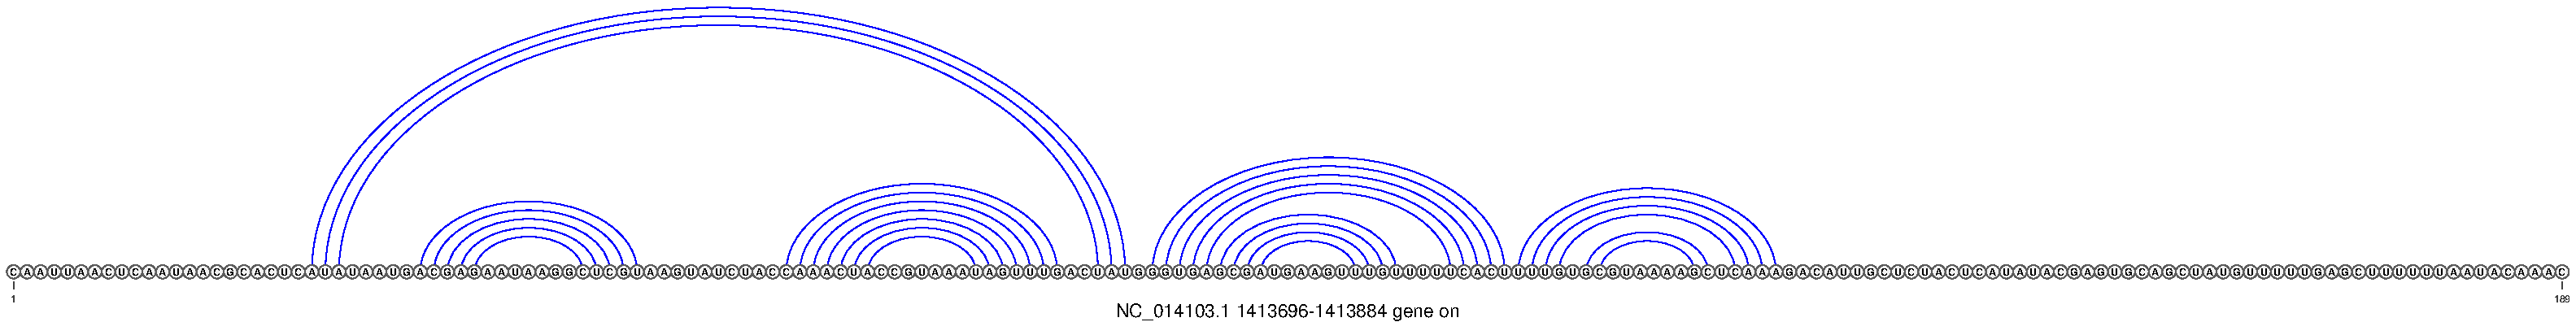
\includegraphics[width=.9\textwidth]{Figures/Ribofinder/NC_014103_1_1413696_1413884_ON.pdf}
\end{subfigure}
\caption{The computationally predicted \rb located upstream of the xpt
gene in {\em B. megaterium} DSM319 (NC\_014103.1 1413696--1413884).
{\em Top:} The gene off conformation. {\em Bottom:} The gene on conformation.}
\label{fig:figure:NC_014103_1_1413696_1413884}
\end{figure}
\medskip

\begin{figure}[!ht]
\centering
\begin{subfigure}[h]{\textwidth}
\centering
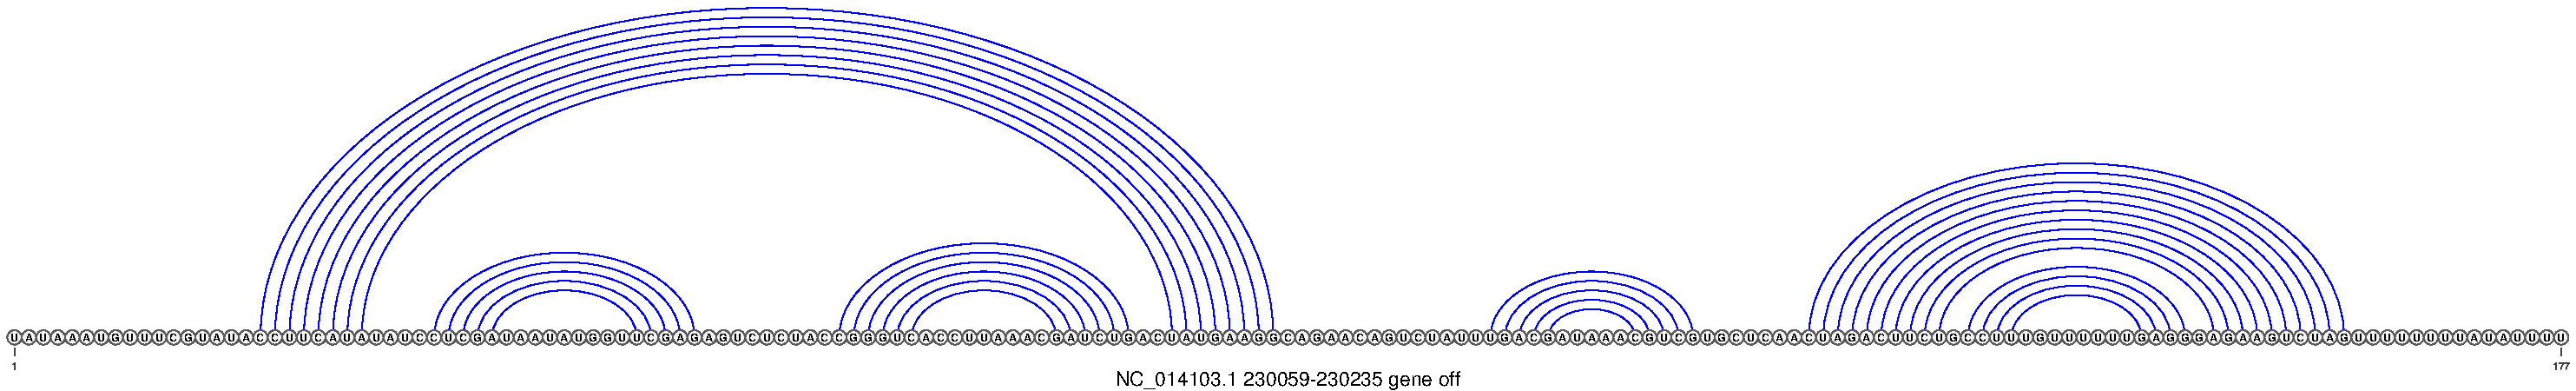
\includegraphics[width=.9\textwidth]{Figures/Ribofinder/NC_014103_1_230059_230235_OFF.pdf}
\end{subfigure} \\
\medskip
\begin{subfigure}[h]{\textwidth}
\centering
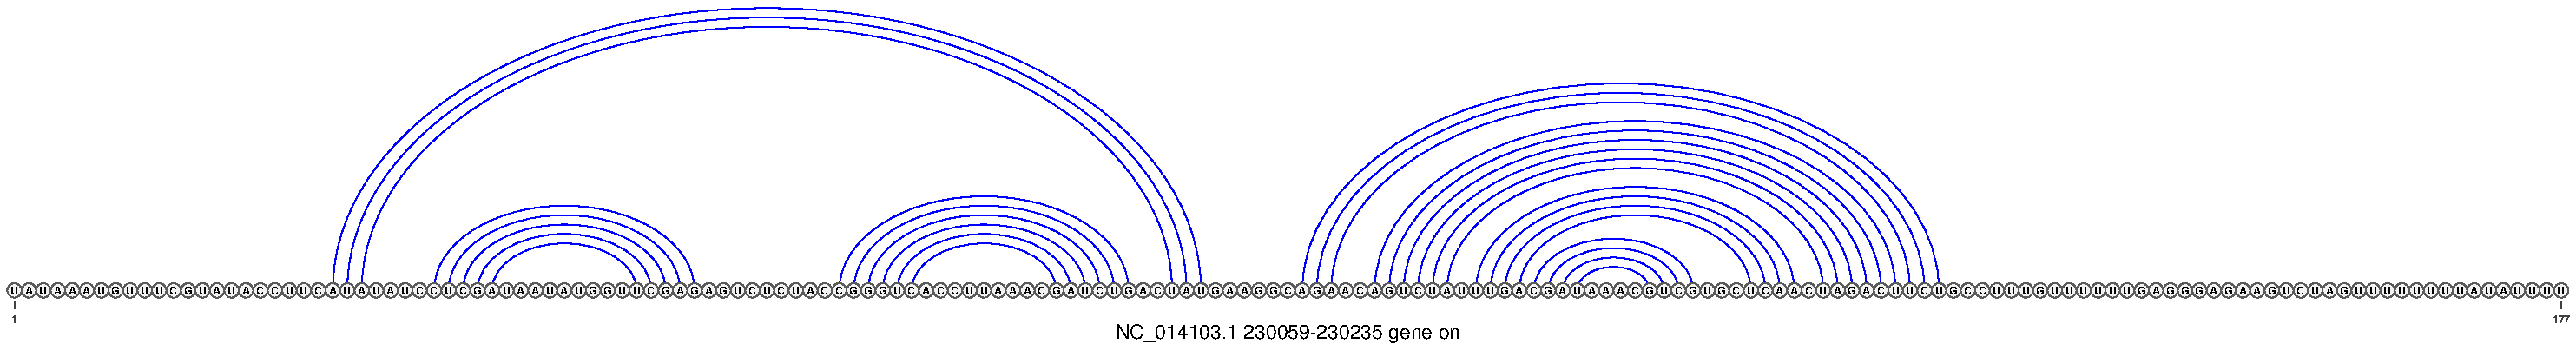
\includegraphics[width=.9\textwidth]{Figures/Ribofinder/NC_014103_1_230059_230235_ON.pdf}
\end{subfigure}
\caption{The computationally predicted \rb located upstream of the GMP synthase
gene in {\em B. megaterium} DSM319 (NC\_014103.1 230059--230235).
{\em Top:} The gene off conformation. {\em Bottom:} The gene on conformation.}
\label{fig:figure:NC_014103_1_230059_230235}
\end{figure}
\medskip

\begin{figure}[!ht]
\centering
\begin{subfigure}[h]{\textwidth}
\centering
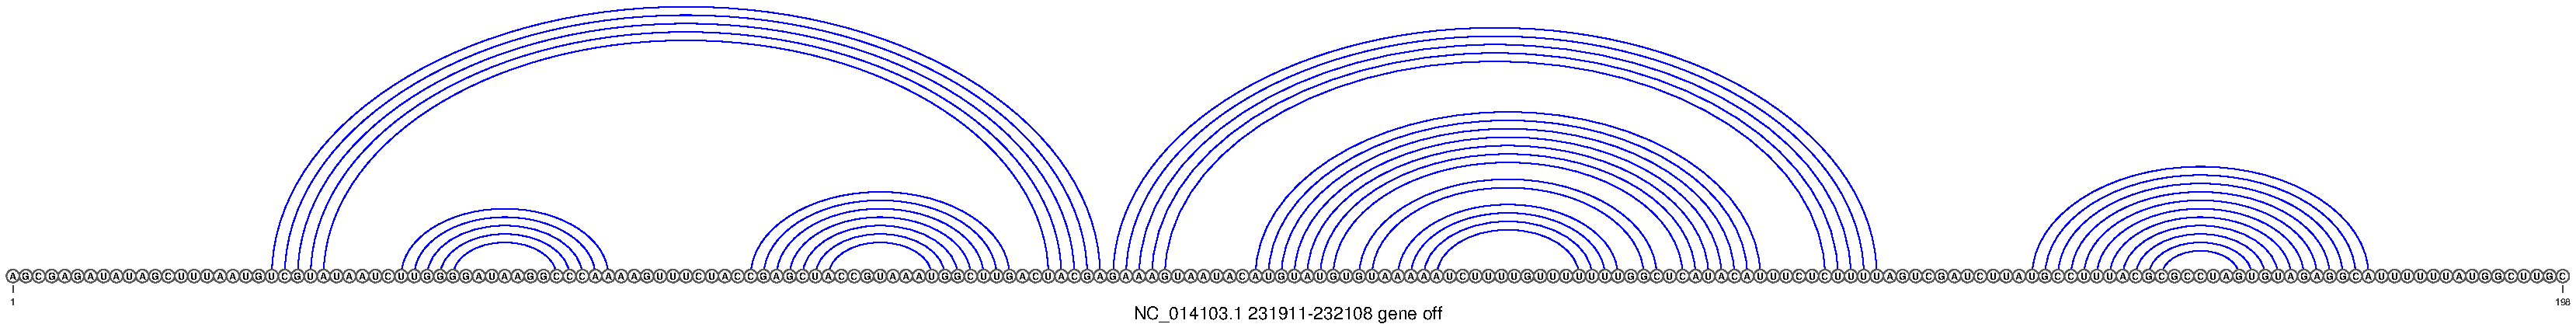
\includegraphics[width=.9\textwidth]{Figures/Ribofinder/NC_014103_1_231911_232108_OFF.pdf}
\end{subfigure} \\
\medskip
\begin{subfigure}[h]{\textwidth}
\centering
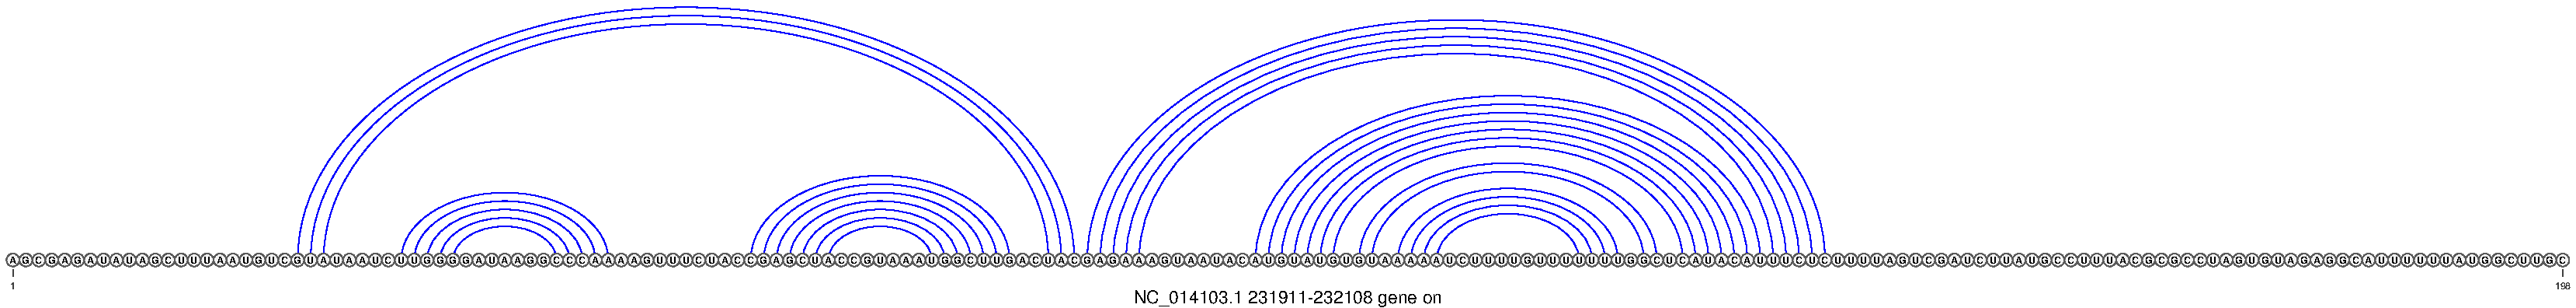
\includegraphics[width=.9\textwidth]{Figures/Ribofinder/NC_014103_1_231911_232108_ON.pdf}
\end{subfigure}
\caption{The computationally predicted \rb located upstream of the guanine permease
gene in {\em B. megaterium} DSM319 (NC\_014103.1 231911--232108).
{\em Top:} The gene off conformation. {\em Bottom:} The gene on conformation.}
\label{fig:figure:NC_014103_1_231911_232108}
\end{figure}
\medskip

\begin{figure}[!ht]
\centering
\begin{subfigure}[h]{\textwidth}
\centering
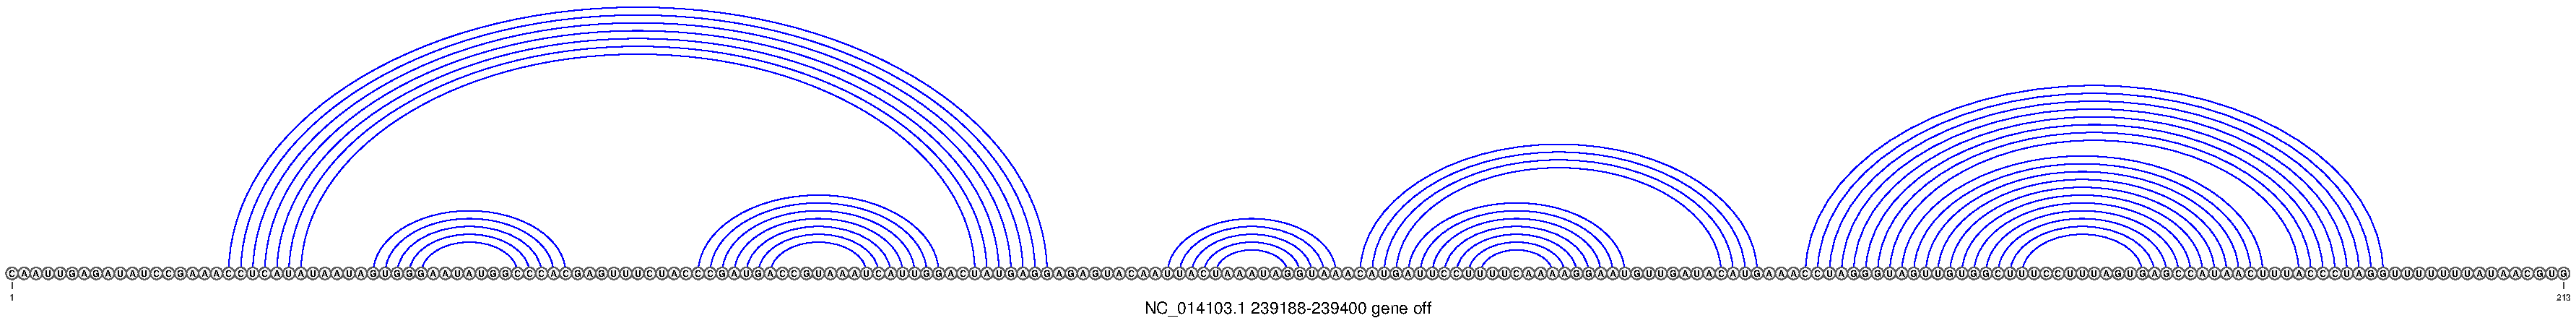
\includegraphics[width=.9\textwidth]{Figures/Ribofinder/NC_014103_1_239188_239400_OFF.pdf}
\end{subfigure} \\
\medskip
\begin{subfigure}[h]{\textwidth}
\centering
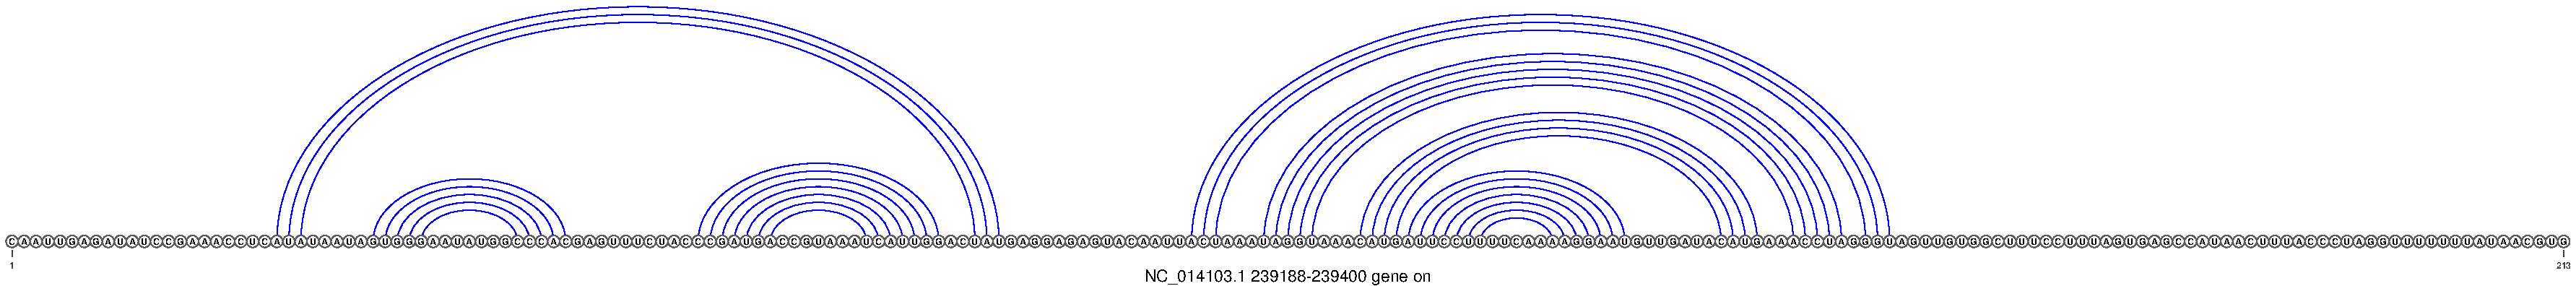
\includegraphics[width=.9\textwidth]{Figures/Ribofinder/NC_014103_1_239188_239400_ON.pdf}
\end{subfigure}
\caption{The computationally predicted \rb located upstream of the
N5-carboxyaminoimidazole
gene in {\em B. megaterium} DSM319 (NC\_014103.1 239188--239400).
{\em Top:} The gene off conformation. {\em Bottom:} The gene on conformation.}
\label{fig:figure:NC_014103_1_239188_239400}
\end{figure}

%!TEX root = ../main.tex

\chapter{FFTbor}
\label{ch:fftbor}

\lhead{FFTbor: Coarse-Grained Energy Landscapes}

\section{Introduction}
\label{sec:fftbor:intro}

In this chapter, we present the \fftbor algorithm and accompanying software.
\fftbor is a novel algorithm developed with the intent of efficiently computing
the Boltzmann probability of those structures which, for a given input RNA
sequence \seq, differ by $k$ base pairs. By leveraging polynomial interpolation
via the \fft, this algorithm runs in \On{4} time and
\On{2} space, a significant improvement over its predecessor. The accompanying
software which implements this algorithm has been used to evaluate the
correlation between kinetic folding speed and landscape ruggedness.

\subsection{Organization}
\label{subsec:fftbor:org}

This chapter is organized in the following fashion. First, we provide
background on
the problem which \fftbor aims to address, as well as a brief overview of
existing approaches. We follow by a formal explanation of the problem, and
proceed to describe how the energy landscape is coarsified into discrete bins.
We then develop the recursions for the parameterized partition function using
the Nussinov-Jacobson energy model, which allows us to highlight the novel aspects
of the algorithm. After developing the recursions, we indicate how they can be
reformulated as a polynomial whose coefficients $z_k=\bfZ{k}{1,n}$. We then
describe how the \fft can be employed to efficiently compute the coefficients
$z_k$, finishing our description of the underlying algorithm. Then we proceed
to present an application of \fftbor, in the area of RNA folding kinetics.

\section{Background}
\label{sec:fftbor:bkgrnd}

In \citep{freyhult.b07}, a dynamic programming algorithm
\rnabor---pronounced {\em RNA neighbor}---was developed which simultaneously
computes for
each integer $k$, the Boltzmann probability $\pk = \frac{\bfZ{k}{}}{\fullZ}$
of the subensemble of structures
whose \bpd to a given {\em initial}, or
{\em reference}, structure \strSt is $k$.
\footnote{As later
explained, \fullZ denotes the partition function, defined as the sum of
all Boltzmann factors \boltzf{\str}, over all secondary structures \str
of a given RNA sequence, and $R$ denotes the universal
gas constant and $T$ absolute temperature. Similarly \bfZ{k}{} denotes the
sum of all Boltzmann factors of all structures \str, whose \bpd
to the initial structure \strSt is exactly $k$.}
\rnabor stores the value of the (partial)
partition functions \bfZ{k}{i,j} for all $1 \leq i \leq j \leq n$ and
$0 \leq k \leq n$, each of which requires quadratic time to compute.
Thus it follows that \rnabor runs in time \On{5} and space
\On{3}, which severely limits its applicability to genomic annotation.
This restriction is somewhat mitigated by the fact that
in \citep{cloteloulorenz}, we showed how to use sampling
\citep{ding.nar03} to efficiently approximate
\rnabor in cubic time \On{3} and quadratic space \On{2},
{\em provided} that the starting structure \strSt is the \mfe
(MFE) structure. We expect that a more efficient version of
\rnabor could be used in applications in genomics and synthetic
biology, to detect potential conformational switches---
RNA sequences containing two or more (distinct) metastable structures.

In this chapter, we describe a radically different algorithm, \fftbor
\citep{senter.po12},
prounounced {\em FFT neighbor},
that uses polynomial interpolation to compute the
coefficients $p_0,\ldots,p_{n-1}$ of the polynomial defined in
\eqnref{fftbor:pOfX},
where \pk is defined by $\pk = \frac{\bfZ{k}{}}{\fullZ}$.
Due to severe numerical instability issues in both the Lagrange
interpolation formula and in Gaussian elimination, we employ
the \fft (FFT) to compute the \idft (DFT) on values $y_0,\ldots,y_{n-1}$,
where $y_k = p(\omega^k)$ and
$\omega = \pRoU$ is the principal \nRoU and
$p(x)$ is defined in \eqnref{fftbor:pOfX}. This
gives rise to an improved version of \rnabor, denoted \fftbor,
which runs in time \On{4} and space \On{2}.

\section{Formalization of the problem}
\label{sec:fftbor:formal}

\fftbor aims to compute the coefficients $p_0,\dots,p_{n-1}$ of the polynomial

\begin{align}
\label{eq:fftbor:pOfX}
p(x) = p_0 + p_1 x + p_2 x^2 + \dots + p_{n-1} x^{n-1},
\end{align}

where \pk is defined as $\pk = \frac{\bfZ{k}{}}{\fullZ}$. We employ the \fft to compute
the \idft on values $y_0,\dots,y_{n-1}$, where
$y_k = p(\omega^k)$ and $\omega = \pRoU$ is the principal \nRoU and $p(x)$ is defined in
\eqnref{fftbor:pOfX}. By leveraging
\nRoUs in conjunction with the \idft the we subvert numeric instability
issues observed with both Lagrange interpolation and Gaussian elimination.

Consider an RNA sequence $\seq = \seqN$, where
$s_i \in \{\text{A,\,U,\,G,\,C}\}$, i.e. a sequence of nucleotides. We can describe a
secondary structure \str which is compatible with \seq as a collection of
base pair tuples $(i,j)$, where $1 \le i \le i+\theta < j \le n$ and
$\theta \ge 0$ (generally taken to be $3$), the minimum number of unpaired bases
in a hairpin loop due to steric constraints.

To more simply develop the underlying recursions for \fftbor, we introduce a
number of constraints on the base pairs within \str. Firstly, we require that
each base pair is either a Watson-Crick or G-U wobble, i.e. base pair $(i,j)$
for sequence \seq has corresponding nucleotides $(s_i,s_j)$, which are
restricted to the set

\begin{align}
\label{eq:fftbor:validBP}
\bpSet =
\{\text{(A,\,U),\,(U,\,A),\,(G,\,C),\,(C,\,G),\,(G,\,U),\,(U,\,G)}\}.
\end{align}

With
this constraint satisfied we say that \str is {\em compatible} with \seq, and
for the remainder of this chapter will only consider those structures which are
compatible with \seq.
Secondly, we insist that given two base pairs $(i,j), (x,y)$ from \str,
$i=x \iff j=y$ (bases have at most one partner). Finally, we require that
$i<x<j \iff i<y<j$ (no pseudoknots are allowed). While pseudoknots have been
shown to be present in some biologically relevant RNAs, their inclusion greatly
complicates the recursive decomposition of the structure, and thus it is common
to ignore them.

Provided two secondary structures \strST, we can define a notion of
distance between them. There are a number of different definitions of distance
used across the literature; we will use {\em \bpd} for \fftbor.
\Bpd is defined as the symmetric difference between the sets
\strST:

\begin{align}
\label{eq:fftbor:dBP}
\dBP{\str}{\strT} = |\str \cup \strT| - |\str \cap \strT|.
\end{align}

Given this definition of distance, two structures \str and \strT are said to
be \kNbrs if $\dBP{\str}{\strT} = k$. It is important to note that
the notion of \bpd is also applicable to restrictions of secondary structures
on the subsequence $\seq_{i,j}$,
i.e. $\str_{[i,j]} = \{ (x,y) \,:\, i \leq  x < y \leq j,  (x,y) \in \str \}$.

For a restriction of base pairs for a given structure $\str_{[i,j]}$,
$\strT_{[i,j]}$ is said to be a \kNbr of $\str_{[i,j]}$ if

\begin{align}
\label{eq:fftbor:dBPonRestriction}
\dBP{\str_{[i,j]}}{\strT_{[i,j]}} =
|\{ (x,y): i \leq x<y\leq j,
(x,y) \in \str - \strT \text{or} (x,y) \in \strT - \str \}| = k.
\end{align}

\section{Derivation of the \fftbor algorithm}
\label{sec:fftbor:math}

Given an RNA sequence $\seq=\seqN$ and compatible secondary structure
\strSt, let \bfZ{k}{} denote the sum of the Boltzmann factors
\boltzf{\str} of all \kNbrs \str of \strSt; i.e.

\begin{align}
\bfZ{k}{} = \bfZ{k}{1,n} =
\sum_{\mathclap{\substack{\str \text{ such that } \rule[-.5ex]{0pt}{0pt} \\
 \dBP{\str}{\strSt}=k}}}\;
\boltzF{\str}
\end{align}

where $E(\str)$ denotes the Turner (nearest neighbor)
energy \citep{xia:RNA}
of \str, $R = 0.00198$ kcal/mol denotes the universal
gas constant and $T$ denotes absolute temperature. From this, it follows that
the full partition function is defined as

\begin{align}
\label{eq:fftbor:partFunc}
\fullZ = \bfZ{}{1,n} = \sum_{k=0}^n \bfZ{k}{1,n}
\end{align}

since the \bpd between \strSt and \str is at most

\begin{align}
\label{eq:fftbor:maxDist}
\dBP{\strSt}{\str} \leq |\strSt| + \lfloor \frac{n-\theta}{2} \rfloor \leq n.
\end{align}

We can then define the Boltzmann probability of all \kNbrs of \strSt as

\begin{align}
\label{eq:fftbor:probK}
p(k) =\frac{\bfZ{k}{1,n}}{\bfZ{}{1,n}}.
\end{align}

By visualizing the probabilities \pk as a function of $k$, we generate a
coarse-grained view of the one-dimensional energy landscape of \seq with
respect to \strSt. When \strSt is taken to be the \mfes for example, one would
anticipate to see a peak at $k=0$, with additional peaks implying additional
metastable structures; local energy minima which could suggest an energetic
trap while folding.

\subsection{Definition of the partition function
\texorpdfstring{\bfZ{k}{1,n}}{}}
\label{subsec:fftbor:recursions}

For the rest of the chapter, we consider both \seq as well as the
secondary structure \strSt on \seq to be fixed. We now recall the
recursions from Freyhult et al. \citep{Freyhult.ab05} to determine
the partition function \bfZ{k}{i,j} with
respect to the Nussinov-Jacobson
energy $E_0$ model \citep{nussinovjacobson}, defined by
$-1$ times the number of base pairs; i.e. $E_0(S) = -1 \cdot |S|$.
Although we describe here the recursions for the Nussinov-Jacobson
model, for the sake of
simplicity of exposition, both \rnabor
\citep{Freyhult.ab05} as well as our current software \fftbor,
concern the Turner energy model (described in \Secref{sec:fftbor:turner}), consisting of free energy parameters for
stacked bases, hairpins, bulges, internal loops and multiloops.

% The full
% recursions for \fftbor are described for the
% the Turner energy model in the appendix.

The base case for \bfZ{k}{i,j} is given by

\begin{align}
\label{eq:fftbor:initZpart1}
\bfZ{0}{i,j} = 1, \text{ for } i \le j,
\end{align}

since the only $0$-neighbor to a structure \strSt
is the structure \strSt itself, and

\begin{align}
\label{eq:fftbor:initZpart2}
\bfZ{k}{i,j} = 0, \text{ for } k > 0, i \le j \leq i + \theta,
\end{align}

since the empty structure is the only possible structure for a
sequence shorter than $\theta + 2$ nucleotides, and so there are no
\kNbrs for $k>0$. The recursion used to compute
\bfZ{k}{i,j} for $k > 0$ and $j > i+\theta$ is

\begin{align}
\label{eq:fftbor:bfZkij}
\bfZ{k}{i,j} = \bfZ{k-b_0}{i,j-1}\enspace +
\sum_{\substack{(s_r,s_j) \in \bpSet, \\ i \leq r<j}}\qquad
\sum_{\mathclap{w+w'=k-b(r)}}\enspace
\exp(-E_0(r,j)/RT) \cdot \bfZ{w}{i,r-1} \bfZ{w'}{r+1,j-1},
\end{align}

where $E_0(r,j) = -1$ if positions $r,j$ can pair in sequence \seq,
and otherwise $E_0(r,j) = +\infty$. Additionally,
$b_0 = 1$ if $j$ is base-paired
in $\strSt_{[i,j]}$ and $0$ otherwise, and
$b(r)=\dBP{\strSt_{[i,j]}}{\strSt_{[i,r-1]} \cup \strSt_{[r+1,j-1]} \cup\{(r,j)\}}$.
This holds since in a secondary
structure $\strT_{[i,j]}$ on \seqIJ that is a \kNbr of
$\strSt_{[i,j]}$,
either nucleotide $j$ is unpaired in $[i,j]$ or it is
paired to a nucleotide $r$ such that $i \leq r < j$. In this
latter case it is enough to study the smaller sequence segments
$[i,r-1]$ and $[r+1,j-1]$ noting that, except for $(r,j)$,
base pairs outside of these regions are not allowed, since there
are no pseudoknots. In addition,
for $\dBP{\strSt_{[i,j]}}{\strT_{[i,j]}} = k$ to hold,
it is necessary for $w+w' = k -b(r)$ to hold, where $w =
\dBP{\strSt_{[i,r-1]}}{\strT_{[i,r-1]}}$ and $w' =
\dBP{\strSt_{[r+1,j-1]}}{\strT_{[r+1,j-1]}}$, since $b(r)$ is the
number of base pairs that differ between $\strSt_{[i,j]}$ and a
structure $\strT_{[i,j]}$, due to the introduction of the base pair
$(r,j)$.

Given RNA sequence \seq and compatible initial structure \strSt,
we define the {\em polynomial}

\begin{align}
\label{eq:fftbor:zOfX}
\fullZx = \sum_{k=0}^n z_k x^k
\end{align}

where coefficients $z_k=\bfZ{k}{1,n}$. Moreover, because of
\eqnref{fftbor:maxDist} and the fact that the minimum number of
unpaired bases in a hairpin loop $\theta$ is $3$, we know that $z_n=0$,
so that \fullZx is a polynomial of degree strictly less than $n$.
If we evaluate the polynomial \fullZx for $n$ distinct values

\begin{align}
\label{eq:fftbor:solutionsForAlpha}
\emZof{}{a_1} = y_1, \dots, \emZof{}{a_n} = y_n,
\end{align}

then the Lagrange polynomial interpolation formula guarantees that
$\fullZx = \sum_{k=1}^n y_k P_k(x)$, where the polynomials $P_k(x)$ have degree
at most $n-1$ and are given by the Lagrange formula

\begin{align}
\label{eq:fftbor:lagrangeInterpolation}
P_k(x) = \frac{\prod_{i\ne k} (x-x_i)}{\prod_{i \ne k} (x_k-x_i)}.
\end{align}

Since the polynomials $P_k(x)$ can be explicitly computed, it follows that
we can compute the coefficients $z_k$ of polynomial \fullZx. As we describe
below, the evaluation of \fullZx for a fixed value of $x$ can be done in
time \On{3} and space \On{2}.  It follows that the coefficients
$z_k=\bfZ{k}{1,n}$ can be computed after
$n$ evaluations of \fullZx, where the space for each evaluation of \fullZx
is re-used; hence these evaluations can be performed in time \On{4} and space
\On{2}. Finally,
Lagrange interpolation is clearly computable in time \On{3}.
Although this approach is theoretically sound, there are severe
numerical stability issues related to the interpolation method
\citep{highambarycentricinterpolation},
the choice of values $a_1,\dots,a_{n}$ in the interpolation,
and floating point arithmetic (round-off error) related to the
astronomically large values of the partition functions
\bfZ{k}{1,n}, for $0 \leq k < n$. After many unsuccessful
approaches including scaling we obtained excellent results by
interpolating the polynomial $p(x)$, defined in \eqnref{fftbor:pOfX},
rather than the polynomial \fullZx, defined in \eqnref{fftbor:zOfX},
and performing interpolation with the \fft (FFT) \citep{cormen}
where \alphaN are
chosen to be \nRoUs,
$\alpha_k = \kRoU$.
One
advantage of the FFT is that interpolation can be performed in $O(n \log n)$
time, rather than the cubic time required by using the Lagrange formula
shown in \eqnref{fftbor:lagrangeInterpolation} or by Gaussian elimination. Fewer
numerical operations implies increased numerical stability in our application.

\subsection{Recursions to compute the polynomial
\texorpdfstring{\emZ{i,j}}{}}
\label{subsec:fftbor:polynomial}

Given an initial secondary structure \strSt of a
given RNA sequence \seq, our goal is to compute

\begin{align}
\label{eq:fftbor:defZofK}
\bfZ{k}{1,n} = \sum_{\mathclap{\substack{\str \text{ such that }\\ \dBP{\str}{\strSt}=k}}}\;
\boltzNuss{\str}
\end{align}

where \str can be any structure compatible with \seq.
As previously mentioned, the recurrence relation for \rnabor
with respect to the Nussinov energy model $E_0$ is

\begin{align}
\label{eq:fftbor:rnaborNuss}
\bfZ{k}{i,j} = \bfZ{k-b_0}{i,j-1}\enspace +
\sum_{\substack{(s_r,s_j) \in \bpSet, \\ i \le r<j}}
\left(
\boltzNuss{r,j}\enspace \sum_{\mathclap{w+w'=k-b(r)}}\quad
\bfZ{w}{i,r-1} \bfZ{w'}{r+1,j-1}
\right)
\end{align}

where $E_0(r,j)=-1$ if $r$ and $j$ can base-pair and otherwise
$+\infty$, and
$b_0 = 1$ if $j$ is base paired in $\strSt_{[i,j]}$ and $0$ otherwise, and
$b(r)=\dBP{\strSt_{[i,j]}}{\strSt_{[i,r-1]} \cup \strSt_{[r+1,j-1]} \cup\{(r,j)\}}$.
The following theorem shows that an analogous recursion can be used to compute
the {\em polynomial} $\emZ{i,j}$ defined by

\begin{align}
\label{eq:fftbor:polynomialZij}
\emZ{i,j} = \sum_{k=0}^n z_k(i,j)\,x^k
\end{align}

where

\begin{align}
z_k(i,j)\>=\>
\bfZ{k}{i,j}\enspace=\enspace
\sum_{\mathclap{\substack{\str \text{ such that } \\
\dBP{\str}{\strSt_{[i,j]}}=k}}}\enspace
\boltzNuss{\str}.
\end{align}

Here, in the summation, \str runs over structures on \seqIJ, which
are \kNbrs of the restriction $\strSt_{[i,j]}$ of initial structure
\strSt to interval $[i,j]$, and
$E_0(S)=-1 \cdot |S|$ denotes the Nussinov-Jacobson energy of \str.

\begin{theorem}
\label{thm:fftbor:recursions}
Let \seqN be a given RNA sequence.
For any integers $1 \leq i \leq j \leq n$, let

\begin{align}
\emZ{i,j} = \sum_{k=0}^n z_k\,x^k
\end{align}

where

\begin{align}
z_k(i,j) = \bfZ{k}{i,j}.
\end{align}

Then for $i\leq j \leq i+\theta$, $\emZ{i,j}=1$ and for
$j>i+\theta$ we have the recurrence relation

\begin{align}
\label{eq:fftbor:fftborNussPoly}
\emZ{i,j} = \emZ{i,j-1} \cdot x^{b_0} +
\sum_{\substack{(s_r,s_j) \in \bpSet, \\ i\le r<j}}
\left(
\boltzNuss{r,j} \cdot \emZ{i,r-1} \cdot \emZ{r+1,j-1} \cdot x^{b(r)}
\right).
\end{align}

where $b_0 = 1$ if $j$ is base-paired in $\strSt_{[i,j]}$ and $0$ otherwise, and
$b(r) =
\dBP{\strSt_{[i,j]}}{\strSt_{[i,r-1]} \cup \strSt_{[r+1,j-1]} \cup \{(r,j)\}}$.
\end{theorem}

\begin{proof}
First, some notation is necessary.
Recall that if $F$ is an arbitrary
polynomial [resp. analytic] function, then $[x^k]F(x)$
denotes the coefficient of $x^k$ [resp. the $k$th Taylor coefficient in the
Taylor expansion of $F(x)$]. For instance, in
\eqnref{fftbor:pOfX}, $[x^k]p(x) = \pk$, and in
\eqnref{fftbor:zOfX}, $[x^k]\fullZx = z_k$.

By definition, it is clear that $\emZ{i,j}=1$ if $i \leq j \leq i + \theta$,
where we recall that $\theta = 3$ is the minimum number of unpaired bases in
a hairpin loop. For $j > i + \theta$, we have

\begin{align}
\begin{split}
[x^k] \emZ{i,j} &= z_k(i,j) = \bfZ{k}{i,j} \\
&= \bfZ{k-b_0}{i,j-1} +
\sum_{r=i}^{j-1}\hspace{2.25em} \sum_{\mathclap{k_0+k_1=k-b(r)}}\hspace{1.5em}
\left( \boltzNuss{r,j} \cdot \bfZ{k_0}{i,r-1} \cdot \bfZ{k_1}{r+1,j-1} \right) \\
&= [x^{k-b_0}] \emZ{i,j-1} \\
&+ \sum_{r=i}^{j-1}\hspace{2.25em} \sum_{\mathclap{k_0+k_1=k-b(r)}}\hspace{1.5em}
\left( \boltzNuss{r,j} \cdot \left( [x^{k_0}] \emZ{i,r-1} \right) \cdot
\left( [x^{k_1}] \emZ{r+1,j-1} \right) \right) \\
&= [x^{k-b_0}] \emZ{i,j-1} \\
&+ \sum_{r=i}^{j-1}\hspace{2.25em} \sum_{\mathclap{k_0+k_1=k-b(r)}}\hspace{1.5em}
\left( \boltzNuss{r,j} \cdot [x^{k_0+k_1}]
\left( \emZ{i,r-1} \cdot \emZ{r+1,j-1} \right) \right).\\
\end{split}
\end{align}

By induction, the proof of the theorem now follows.
\end{proof}

Notice that if one were to compute all terms of the polynomial $\emZ{1,n}$
by explicitly performing polynomial multiplications,
then the computation would require \On{5} time and \On{3} space.
Instead of explicitly performing polynomial expansion in {\em variable} $x$,
we instantiate $x$ to a fixed complex number $\alpha \in \mathbb{C}$, and apply
the following recursion for this instantiation:

\begin{align}
\label{eq:fftbor:fftborNussPolyAlpha}
\emZof{i,j}{\alpha} = \emZof{i,j-1}{\alpha} \cdot \alpha^{b_0} +
\sum_{\substack{(s_r,s_j) \in \bpSet, \\ i \le r<j}}
\left(
\boltzNuss{r,j} \cdot
\emZof{i,r-1}{\alpha} \cdot \emZof{r+1,j-1}{\alpha} \cdot \alpha^{b(r)}
\right).
\end{align}

In this fashion, we can compute $\emZof{}{\alpha}=\emZof{1,n}{\alpha}$ in
\On{3} time and \On{2} space. For $n$ distinct complex values
\alphaN, we can compute and save only the
values $\emZof{}{\alpha_0},\dots,\emZof{}{\alpha_{n-1}}$, each time re-using the
\On{2} space for the next computation of $\emZof{}{\alpha_k}$. It follows that
the computation resources used to determine the (column) vector

\begin{align}
\label{eq:fftbor:yColumn}
\bfY = (y_0,\dots,y_{n-1})^{\text T} =
\left(
\begin{array}{l}
y_0 \\
y_1 \\
\vdots \\
y_{n-1} \\
\end{array}
\right)
\end{align}

where
$y_0=\emZof{}{\alpha_0},\dots,y_{n-1}=\emZof{}{\alpha_{n-1}}$ is thus quartic time \On{4} and quadratic space \On{2}.

\subsection{Polynomial interpolation to evaluate
\texorpdfstring{\emZ{i,j}}{}}
\label{subsec:fftbor:fft}

Let $\omega = \pRoU$ be the principal \nRoU.
Recall that the Vandermonde matrix $V_n$ is defined to be the
$n \times n$ matrix, whose $i,j$ entry is $\omega^{i \cdot j}$; i.e.

\begin{align}
\label{eq:fftbor:vandermonde}
V_n =
\left(
\begin{array}{rrrrr}
1 & 1 & 1 & \dots & 1 \\
1 & \omega & \omega^2 & \dots & \omega^{n-1} \\
1 & \omega^2 & \omega^4 & \dots & \omega^{2(n-1)} \\
1 & \omega^3 & \omega^6 & \dots & \omega^{3(n-1)} \\
\vdots & \vdots & \vdots & \vdots & \vdots \\
1 & \omega^{n-1} & \omega^{2(n-1)} & \dots & \omega^{(n-1)(n-1)} \\
\end{array}
\right)
\end{align}

The \fft is defined to be the $O(n \log n)$
algorithm to compute the Discrete Fourier Transform (DFT), defined
as the matrix product $\bfY = V_n {\bf A}$:

\begin{align}
\label{eq:fftbor:dftMatrix}
\left(
\begin{array}{l}
y_0 \\
y_1 \\
y_2 \\
\vdots \\
y_{n-1} \\
\end{array}
\right)
= V_n \cdot
\left(
\begin{array}{l}
a_0 \\
a_1 \\
a_2 \\
\vdots \\
a_{n-1} \\
\end{array}
\right)
\end{align}

On page $837$ of \citep{cormen}, it is shown that the
$(i,j)$ entry of $V_n^{-1}$ is $\frac{\omega^{-j i}}{n}$
and that

\begin{align}
\label{eq:fftbor:aFromY}
a_j = \frac{1}{n} \sum_{k=0}^{n-1} y_k\,\omega^{-kj}
\end{align}

for $j=0,\dots,n-1$.

Since we defined \bfY in \eqnref{fftbor:yColumn} by $\bfY =
(y_0,\dots,y_{n-1})^{\text T}$, where
$y_0=\emZof{}{\alpha_0},\dots,y_{n-1}=\emZof{}{\alpha_{n-1}}$
and $\alpha_k = \omega^k \kRoU$, it follows that the coefficients
$z_k=\bfZ{k}{1,n}$ in the polynomial
$\fullZx = z_0 + z_1 x + \dots + z_{n-1} x^{n-1}$ defined in
\eqnref{fftbor:zOfX} can be computed, at least in principle,
by using the \fft. It turns out, however, that the values of
\bfZ{k}{1,n} are so astronomically large, that the ensuing numerical
instability makes even this approach infeasible for values of $n$
that exceed $56$ (data not shown).
Nevertheless, our approach can be modified as follows.
Define \bfY by $\bfY = (y_1,\dots,y_n)^{\text T}$, where
$y_1=\frac{\emZof{}{\alpha_1}}{\fullZ},\dots,
y_{n}=\frac{\emZof{}{\alpha_n}}{\fullZ}$, and
\fullZ is the partition function defined in \eqnref{fftbor:partFunc}.
Using the \fft to compute the \idft, it follows from
\eqnref{fftbor:aFromY} that we can compute the probabilities $p_0,\dots,p_{n-1}$
that are coefficients of the polynomial
$p(x) = p_0 + p_1 x + \dots + p_{n-1}x^{n-1}$
defined in \eqnref{fftbor:pOfX}. For genomics applications, we are
only interested in the $m$ most significant digits of each \pk, as described
in the pseudocode on the following page.
\medskip

\begin{figure}[!ht]
\hrule \rule[0ex]{0pt}{0pt}
\begin{center}
{\large Pseudocode for \fftbor} \\
\end{center}
\begin{tabular*}{\textwidth}{ll}
{\sc Purpose:} & Computes the $m$ most significant digits
of probabilities $\pk = \sfrac{\bfZ{k}{1,n}}{\fullZ}$ \rule[-1.5ex]{0pt}{0pt} \\
{\sc Input:} & RNA sequence $\seq = \seqN$, secondary
structure \strSt of \seq, integer $m$ \rule[-1.5ex]{0pt}{0pt} \\
{\sc Output:} & Probabilities $\pk = \sfrac{\bfZ{k}{1,n}}{\fullZ}$ to $m$ significant digits for $k=0,\dots,n-1$ \rule[-1.75em]{0pt}{0pt} \\
\hline \rule[0ex]{0pt}{0pt}
\end{tabular*}
\begin{algorithmic}[1]
\Function{FFTbor}{\seq, \strSt, $m$}
\State $n \gets \textit{length}(\seq)$
\For{$k \gets 0, n-1$}
\Comment{Compute all \nRoUs}
\State $\omega_k \gets \exp(\frac{2 \pi i k}{n})$
\EndFor
\For{$k \gets 0, n-1$}
\Comment{Note that $\emZof{}{\omega_0} = \fullZ$}
\State $y_k \gets 10^m \cdot \frac{\emZof{}{\omega_k}}{\emZof{}{\omega_0}}$
\EndFor
\For{$k \gets 0, n-1$}
\Comment{Compute IDFT from \eqnref{fftbor:aFromY}}
\State $a_k \gets \frac{1}{n} \sum_{j=0}^{n-1} y_j\, \omega^{-kj}$
\State $\pk \gets 10^{-m} \cdot \lfloor a_k \rfloor$
\Comment{Truncate to $m$ significant digits}
\EndFor
\State \textbf{return} $p_0,\dots,p_{n-1}$
\Comment{Return all \pk for $0 \leq k < n$,
from \eqnref{fftbor:probK}}
\EndFunction
\rule[-0.35ex]{0pt}{0pt}
\end{algorithmic}
\caption[Pseudocode for \fftbor]{The function {\sc FFTbor} computes the $m$ most significant digits
of $p_0,\dots,p_{n-1}$, where $\pk = \frac{\bfZ{k}{}}{\fullZ}$. This algorithm
operates in \On{4} time and \On{2} space, a significant improvement over its
predecessor \rnabor.}
\label{fig:fftbor:algo}
\rule[0ex]{0pt}{1.5em} \hrule
\end{figure}

\section{Benchmarking and performance considerations}
\label{sec:fftbor:benchmarking}

In this subsection, we show that we need only evaluate the polynomial
\fullZx, as defined in
\eqnref{fftbor:zOfX}, for $n/2$ of the \nRoUs.
 It is first necessary to recall the definition of complex
conjugate.
Recall that the complex conjugate of $z$ is denoted by $\overline{z}$;
i.e. if $z=\aPbi$ where $a,b \in \mathbb{R}$ are real numbers and
$i = \sqrt{-1}$,  then $\overline{z} = \aMbi$.

\begin{lemma}
\label{lem:fftbor:compconj}

If \fullZx is the complex polynomial defined in
\eqnref{fftbor:zOfX}, then for any \nRoU
 $\alpha$, it is the case that $\emZof{}{\overline{\alpha}} =
\overline{\emZof{}{\alpha}}$. In other words, if $\alpha$ is a \nRoU
 of the form \aPbi, where $a,b \in \mathbb{R}$ and $b>0$, and
if $\emZof{}{\aPbi} = A + Bi$ where $A,B \in \mathbb{R}$, then it is the case that

\begin{align}
\emZof{}{\aMbi} = A - Bi.
\end{align}

\end{lemma}

\begin{proof}
Letting $i = \sqrt{-1}$, if
$\theta = \frac{2 \pi}{n}$, then
$\omega = e^{i \theta} = \cos(\theta) + i \sin(\theta)$
is the principal \nRoU, and
$e^{(0) \cdot i \theta} = 1 = \omega^{0}, \dots ,
e^{(n-1) \cdot i \theta} = \omega^{n-1}$ together
constitute the complete collection of all
\nRoUs---i.e. the $n$ unique solutions of
of the equation $x^n -1 = 0$ over the field $\mathbb{C}$ of complex numbers.
Clearly, for any $1 \leq k < n$,
$e^{-i k \theta} = 1 \cdot e^{-i k \theta} =
e^{2 \pi i} \cdot e^{-i k \theta} = e^{i(2 \pi - k \theta)} =
e^{i(n \theta - k \theta)} = e^{i \theta (n - k)}$.
Moreover, if $\omega^k = e^{i k \theta} = a + b i$ where
$b>0$, then we have $e^{-i k \theta} = \aMbi$. It follows that for any
\nRoU of the form \aPbi, where $b>0$, the number \aMbi
is also an \nRoU.

Recall that $\fullZx = \sum_{k=0}^n z_k x^k$, where
$z_k \in \mathbb{R}$ are real numbers representing the partition function
\bfZ{k}{1,n} over
all secondary structures of a given RNA sequence \seqN,
whose \bpd from initial structure
\strSt is $k$. Thus, in order to prove the lemma, it suffices to show
that for all values $k=0,\dots,n-1$, if \aPbi is a
\nRoU, where $a,b \in \mathbb{R}$
and $b>0$, and if $(\aPbi)^k = C+Di$ where $C,D \in \mathbb{R}$, {\em then}
$(\aMbi)^k = C-Di$. Indeed, we have the following.

\begin{align}
\begin{split}
(\aPbi)^m &= \sum_{k=0}^m \binom{m}{k}\; a^{m-k} \cdot (bi)^k \\
(bi)^k  &=
\begin{cases}
b^k    & \text{if $k \equiv 0 \bmod 4$} \\
i b^k  & \text{if $k \equiv 1 \bmod 4$} \\
-b^k   & \text{if $k \equiv 2 \bmod 4$} \\
-i b^k & \text{if $k \equiv 3 \bmod 4$} \\
\end{cases}
\end{split}
\end{align}

\begin{align}
\begin{split}
(\aMbi)^m &= \sum_{k=0}^m \binom{m}{k}\; a^{m-k} \cdot (-bi)^k \\
(-bi)^k &=
\begin{cases}
b^k   & \text{if $k \equiv 0 \bmod 4$} \\
-ib^k & \text{if $k \equiv 1 \bmod 4$} \\
-b^k  & \text{if $k \equiv 2 \bmod 4$} \\
ib^k  & \text{if $k \equiv 3 \bmod 4$} \\
\end{cases}
\end{split}
\end{align}

It follows that each term of the form
$a^{m-k} \cdot (bi)^k$, for $k=0,\dots,m$, is the complex conjugate of
$a^{m-k} \cdot (-bi)^k$, and thus $(\aPbi)^m$ is the complex conjugate of
$(\aMbi)^m$. Since \emZof{}{\aPbi} is a sum of terms of the form $z_k (\aPbi)^k$,
it follows that \emZof{}{\aMbi} is the complex conjugate of \emZof{}{\aPbi}.
This completes the proof of the lemma.

\end{proof}

Lemma \ref{lem:fftbor:compconj} immediately entails that we need only to evaluate \fullZx on $n/2$
many of the \nRoUs---namely, those of the form
\aPbi, where $b \geq 0$. The remaining values of \fullZx are obtained by
taking conplex conjugates of the first $n/2$ values. This, along with a
precomputation of powers of the \nRoUs, leads to an
enormous performance speed-up in our implementation of \fftbor.

\section{Coarse-grained kinetics with \fftbor}
\label{sec:fftbor:kinetics}

The output of \fftbor, as shown in
\Figref{fftbor:tppDistributions}, is a probability distribution,
where the $x$-axis represents the \bpd from an arbitrary,
but fixed secondary structure \strSt, and the $y$-axis represents the
Boltzmann probability $p(k) = \frac{\bfZ{k}{}}{\fullZ}$ that a secondary structure
has \bpd $k$ from \strSt. Arguably, this probability distribution
is an accurate one-dimensional projection of the rugged, high dimensional energy
landscape near structure \strSt,
of the sort artistically rendered in the well-known
energy landscape depicted in Figure 1 of \citep{wolynes.ptam05}.
A hypothesis behind theoretical work in biomolecular folding theory in
\citep{bryngelson.p95}
is that kinetic folding slows down as the energy landscape becomes more
{\em rugged}. This is borne out in our computational experiments for RNA
using \fftbor, as reported
in \Figref{fftbor:tppDistributions}.

We randomly chose two TPP \rb
aptamers from the seed alignment for
Rfam family RF$00059$. The first sequence has EMBL accession code
BX$842649.1$ $277414$--$277318$ and is comprised of the $97$ nt sequence
\seqsplit{%
  ACCUGACGCUAGGGGUGUUGGUGAAUUCACCGACUGAGAAUAACCCUUU%
  GAACCUGAUAGAGAUAAUGCUCGCGCAGGGAAGCAAGAAUAGAAAGAU%
}, while the second sequence
has EMBL accession code AACY$022101973.1$ $389$--$487$ and is comprised of the $99$
nt sequence
\seqsplit{%
  UAUAAGUCCAAGGGGUGCCAAUUGGCUGAGAUGGUUUUAACCAAUCCCUU%
  UGAACCUGAUCCGGUUAAUACCGGCGUAGGAAUGGAUUUUCUCUACAGC%
}.
Rfam consensus and \mfess for both sequences are
depicted in \Figref{fftbor:tppConsensusAndMfe}.
Despite the fact that there is no sequence homology according to
pairwise BLAST \citep{blast}, this figure clearly demonstrates that
consensus and
\mfess closely resemble each other, and that the
structures of both TPP \rb aptamers are quite similar, with the
exception of the leftmost hairpin loop [resp. multiloop].
The MFE structures differ
from the consensus structures principally by the addition of base pairs not
determined by covariation in the Rfam alignment.
Indeed, if we let $\str_0,\,\str_1$
denote the Rfam consensus structure [resp. MFE structure] for the $97$ nt
sequence with EMBL accession code BX$842649.1$ $277414$--$277318$, then
$\str_0 \setminus \str_1$ has $4$ base pairs, and $\str_1 \setminus \str_0$
 has $7$
base pairs. If we let $\strT_0,\,\strT_1$
denote the Rfam consensus structure [resp. MFE structure] for the $99$ nt
sequence with EMBL accession code
AACY$022101973.1$ $389$--$487$, then
$\strT_0 \setminus \strT_1$ has $1$ base pair, and $\strT_1 \setminus \strT_0$ has $5$
base pairs.

\begin{figure}[!ht]
\centering
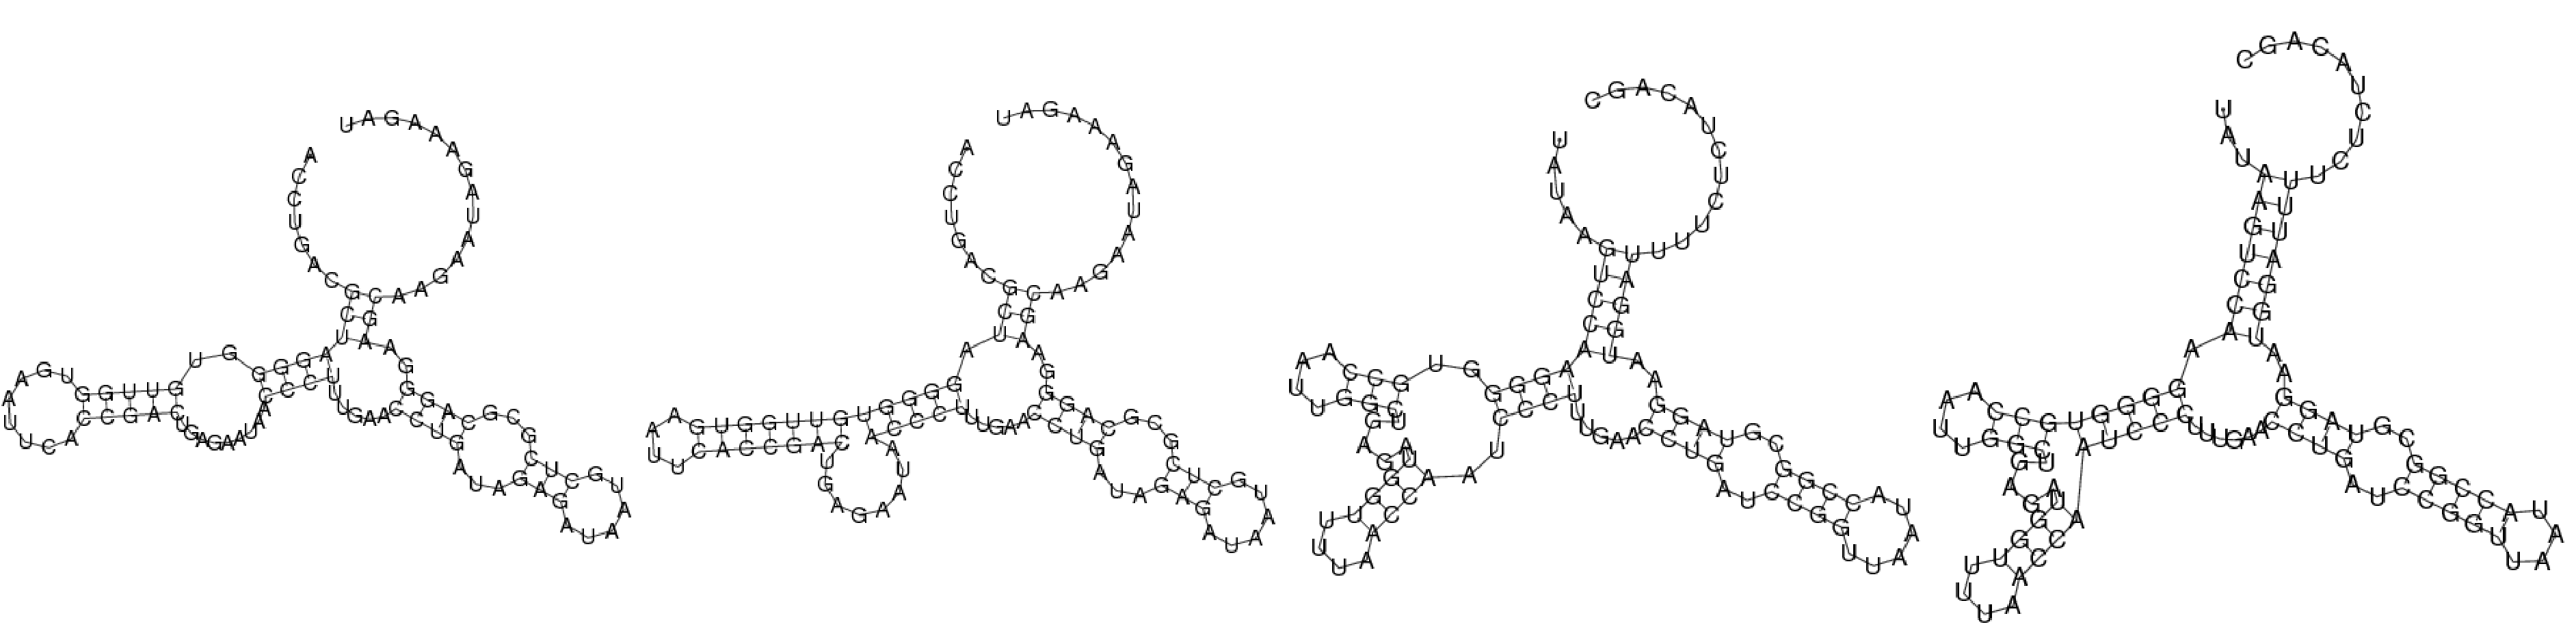
\includegraphics[width=.9\textwidth]{Figures/FFTbor/tppConsensusAndMfe.pdf}
\caption[Rfam consensus structures (Rfam) and \mfe (MFE)
secondary structures for two thiamine pyrophosphate (TPP) \rb aptamers]{Rfam consensus structures (Rfam) and \mfe (MFE)
secondary structures for two thiamine pyrophosphate (TPP) \rb aptamers,
chosen at random from RF$00059$ Rfam family seed alignment
\citep{Gardner.nar11}. Using pairwise BLAST \citep{blast}, there is no
sequence similarity, although the secondary structures are very similar,
as shown in this figure. From left to right:
{\em (A)} MFE structure for BX$842649.1$ $277414$--$277318$.
{\em (B)} Rfam consensus structure for BX$842649.1$ $277414$--$277318$.
{\em (C)} MFE structure for AACY$022101973.1$ $389$--$487$.
{\em (D)} Rfam consensus structure for AACY$022101973.1$ $389$--$487$.
}
\label{fig:fftbor:tppConsensusAndMfe}
\end{figure}

We ran \fftbor on each of the TPP \rb aptamer
sequences, with the MFE structure of each
sequence taken as the initial structure \strSt for that sequence. For the
first sequence, BX$842649.1$ $277414$--$277318$, the \fftbor output
suggests that there are low energy structures
at a distance from the MFE structure, which might compete with the MFE
structure and hence slow the kinetics of folding. In contrast, for the
second sequence, AACY$022101973.1$ $389$--$487$, the \fftbor output suggests
that there are no such competing low energy structures, hence
the second sequence should fold more quickly than the first.

\begin{figure}[!ht]
\centering
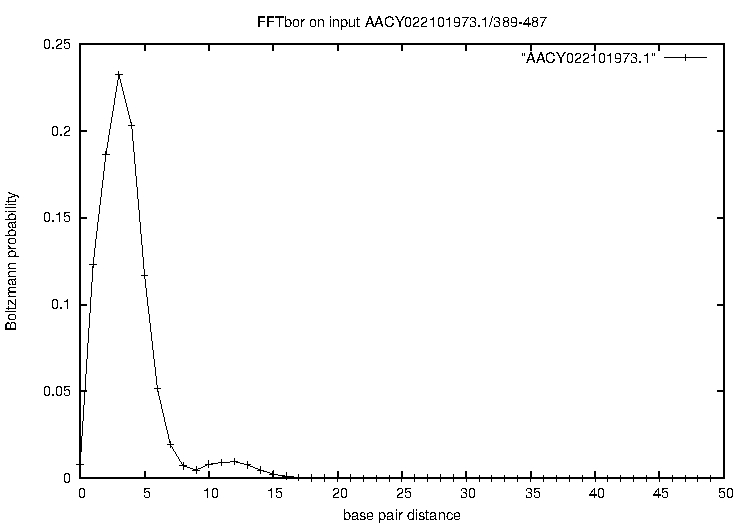
\includegraphics[width=.45\textwidth]{Figures/FFTbor/FFTbor_AACY022101973_1.pdf}
\quad
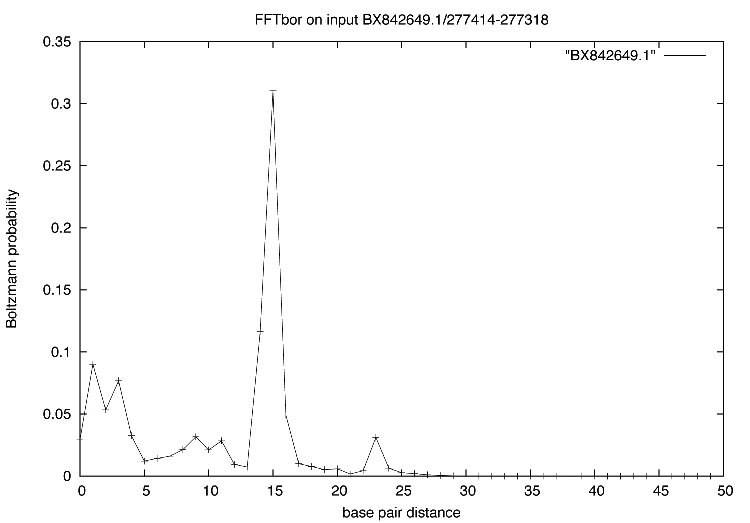
\includegraphics[width=.45\textwidth]{Figures/FFTbor/FFTbor_BX842649_1.pdf}
\caption[Output from \fftbor on two randomly selected
thiamine pyrophosphate \rb (TPP) aptamers]{Output from \fftbor on two randomly selected
thiamine pyrophosphate \rb (TPP) aptamers, taken from the Rfam database
\citep{Gardner.nar11}. The $x$-axis represents \bpd from the
\mfes for each given sequence; the $y$-axis represents
Boltzmann probabilities $p(k) = \frac{\bfZ{k}{}}{\fullZ}$, where
\bfZ{k}{} denotes the sum of Boltzmann factors or all secondary structures,
whose \bpd from the MFE structure is exactly $k$.
{\em (Left)}
The $97$ nt sequence BX$842649.1$ $277414$--$277318$ appears to have a rugged energy
landscape near its \mfes, with distinct
low energy structures that may compete with the MFE structure during the
folding process.
{\em (Right)}
The $99$ nt sequence, AACY$022101973.1$ $389$--$487$ appears to have a smooth energy
landscape near its MFE structure, with no distinct low energy structures
to might compete with the MFE structure.
Based on the \fftbor output or {\em structural profile} near MFE
structure \strSt, one might expect
folding time for the first sequence to increase due to competition from
metastable structures, while one might expect the second sequence to have
rapid folding time.
Computational Monte Carlo folding experiments bear out this fact.
\kinfold \citep{flamm} simulations clearly show that the second
sequence folds
at least four times more quickly than the first sequence. See section
\ref{sec:fftbor:kinetics} for
details.}
\label{fig:fftbor:tppDistributions}
\end{figure}

To test the hypothesis that folding is slower for rugged energy landscapes,
we ran the kinetic folding software, \kinfold \citep{flamm},
on each of the two TPP \rb aptamer sequences,
BX$842649.1$ $277414$--$277318$ and AACY$022101973.1$ $389$--$487$,
to determine the \mfpt (MFPT) to
fold into the MFE structure, when starting from the empty structure.
In this computational
experiment, we took MFPT to be the average number of Monte Carlo steps
taken by \kinfold---each step consisting of the addition or removal
of a single base pair---to fold the
empty structure into the MFE
structure, where the average was taken over $30$ runs, with an absolute
maximum number of Monte Carlo steps taken to be $500,000$.
The first sequence, BX$842649.1$ $277414$--$277318$, converged within $500,000$
steps only for $20$ out of $30$ runs. Assigning the maximum step count of
$500,000$ for the $10$ runs that did not converge, we found a \mfpt
of $311,075.06$ steps for this sequence.
The second sequence, AACY$022101973.1$ $389$--$487$, converged within $500,000$
steps in $29$ out of $30$ runs, and we found a \mfpt of
$61,575.69$ steps for this sequence. From computational experiments of this
type, it is suggestive that \fftbor may prove useful in synthetic
biology,
where one would like to design rapidly folding RNA molecules that
fold into a designated target structure.

In order to more systematically determine the relation between kinetic
folding speed and the ruggedness of an energy landscape near the MFE structure,
we need to numerically quantify ruggedness. To this end, in the following
we define the notion of \ebpd to a designated
structure. Let \strSt be an arbitrary secondary structure of the RNA sequence
$\seq = \seqN$.
The expected \bpd to \strSt is defined by

\begin{align}
E[ \{ \dBP{\str}{\strSt} : \str \in \mathbb{S}(\seqN)\} ] =
\sum_{\str} P(\str) \cdot \dBP{\str}{\strSt}
\end{align}

where
$\mathbb{S}(\seqN)$ denotes the set of secondary structures for
$\seq = \seqN$, $P(\str) = \frac{\boltzf{\str}}{\fullZ}$ is the Boltzmann
probability of \str, and
\dBP{\str}{\strSt} denotes \bpd between \str and \strSt.
If we run \fftbor on an input sequence \seq and secondary structure
\strSt, then clearly
$E[ \{ \dBP{\str}{\strSt} : \str \in \mathbb{S}(\seqN)\} ] =
\sum_{k} k \cdot p(k)$, where $p(k)=\frac{\bfZ{k}{}}{\fullZ}$, obtained from the
program output.  If \strSt is the empty structure, then \fftbor output
is simply the probability distribution of the number of base pairs per
secondary structure, taken over the Boltzmann ensemble of all structures.

For the benchmarking assay, we took all $61$ selenocysteine insertion sequence
(SECIS) sequences from the seed alignment of Rfam family RF$00031$
\citep{Gardner.nar11}. Average length was $64.32 \pm 2.83$ nt.
For each sequence, we ran both \fftbor (when starting
from the empty structure rather than the MFE structure) and a Monte Carlo
folding algorithm, developed by E. Freyhult and P. Clote (unpublished).
Using the Monte Carlo algorithm, we
determined the \mfpt (MFPT), defined as the average
taken over $50$ runs, of the number of Monte Carlo steps taken to fold
the empty structure into the MFE structure, where an absolute upper bound
of $5$ million steps was allowed in the simulation.

Surprisingly, we found that there is a significant
correlation of $0.4847$ with one-tailed
$p$-value of $0.0002$ between the
standard deviation of the \fftbor output (when starting from the
empty structure) and logarithm base $10$ of the \mfpt.
As described above, \fftbor output is simply
the probability distribution
for the number of base pairs per structure, taken over the ensemble
of all secondary structure for the input RNA
sequence. The standard deviation of this probability distribution corresponds
to a notion of the width of the distribution. It is possible that those
sequences having distributions tightly centered around the
mean have faster folding times than those with a wider distribution
due to other local minima causing the RNA to get trapped while folding.

\begin{table}[!ht]
\centering
\begin{tabularx}{\linewidth}{c *{6}{R}}
  \toprule
  ~ & \small{$\mu$} & \small{$\sigma$} & \small{$\sfrac{\sigma}{\mu}$} & \small{$n$} & \small{MFE} & \small{$\log_{10}(\text{MFPT})$} \\
  \cmidrule(l){2-7}
  \small{$\mu$} & $1$ & & & & \\
  \small{$\sigma$} & $-0.4372$ & $1$ & & & \\
  \small{$\sfrac{\sigma}{\mu}$} & $-0.6914$ & $0.9437$ & $1$ & & & \\
  \small{$n$} & $0.7077$ & $-0.1590$ & $-0.3646$ & $1$ & &  \\
  \small{MFE} & $-0.5695$ & $0.7395$ & $0.7596$ & $-0.3685$ & $1$ & \\
  \small{$\log_{10}(\text{MFPT})$} & $-0.0363$ & $0.4844$ & $0.3762$ & $0.4059$ & $0.3990$ & $1$ \\
  % puts data.chomp.split(/\\/).map { |line| line.split("&")[1..-1].map { |item| item.gsub(/\s+/, "") }.reject { |item| item.empty? }.map { |number| "%.4f" % number.to_f }.join(" & ") + " \\\\" }.join(?\n)
  \bottomrule
\end{tabularx}
\caption[Pearson correlation between various aspects of selenocysteine
insertion sequences from the seed alignment of Rfam family
RF$00031$]{\small Pearson correlation between various aspects of selenocysteine
insertion sequences from the seed alignment of Rfam family
RF$00031$ \citep{Gardner.nar11}.
For each of the $61$ RNA sequences, we ran \fftbor, starting
from empty initial structure \strSt, and we ran a Monte Carlo
folding algorithm, developed by E. Freyhult and P. Clote (unpublished).
Using the Monte Carlo algorithm, we
determined the \mfpt (MFPT), defined as the average
taken over $50$ runs, of the number of Monte Carlo steps taken to fold
the empty structure into the MFE structure, where an absolute upper bound
of $5$ million steps was allowed in the simulation.  From the output of
\fftbor, we computed
{\em 1})\, the mean number ($\mu$) of base pairs per structure, taken over
the ensemble of all secondary structures for the given sequence;
{\em 2})\, the standard deviation ($\sigma$) of the number of base pairs per
structure;
{\em 3})\, the coefficient of variation $\frac{\sigma}{\mu}$;
{\em 4})\, the RNA sequence length $n$; and
{\em 5})\, the \mfe (MFE).
Additionally, we computed the logarithm base $10$ of \mfpt
($\log_{10}(\text{MFPT})$), taken over $50$ Monte Carlo runs per sequence
(log base $10$ of the standard deviation of number of Monte Carlo
steps per run was approximately
9\% of $\log_{10}(\text{MFPT})$ on average). The table shows the correlation between each of these aspects.
Some correlations are obvious---for example,
{\em i})\;
the standard deviation $\sigma$ is highly correlated with the
coefficient of variation $\frac{\sigma}{\mu}$;
{\em ii})\;
the mean $\mu$ is negatively correlated with the
coefficient of variation $\frac{\sigma}{\mu}$;
{\em iii})\;
the mean $\mu$ is negatively correlated with the
\mfe (MFE) --- if most low energy structures in the ensemble
have many base pairs, then it is likely that the \mfe is very
low (i.e. since MFE is negative, the absolute value of MFE increases); and
{\em iv})\;
sequence length is negatively correlated with MFE --- as sequence length
increases, the \mfe (MFE) decreases.
However, it may appear surprising that
{\em v})\; the
mean $\mu$ number of base pairs per structure is independent of MFPT
(correlation $-0.0363$), although
{\em vi})\; MFE is correlated with MFPT
(correlation $0.3990$) --- i.e. from {\em (iii)},
lower MFE is correlated with a larger average $\mu$ number of base pairs per
structure, from ({\em vi})
higher MFE is correlated with longer folding time, but
from ({\em v}) the average $\mu$  number of base pairs per structure is
independent of folding time.
The most important insight from this table is that
{\em vii})\;
standard deviation $\sigma$ is correlated with \mfpt---the correlation is statistically significant, with one-tailed
$p$-value of $0.0002$.}
\label{table:correlationFFTborEmpty}
\end{table}

\begin{figure}[!ht]
\centering
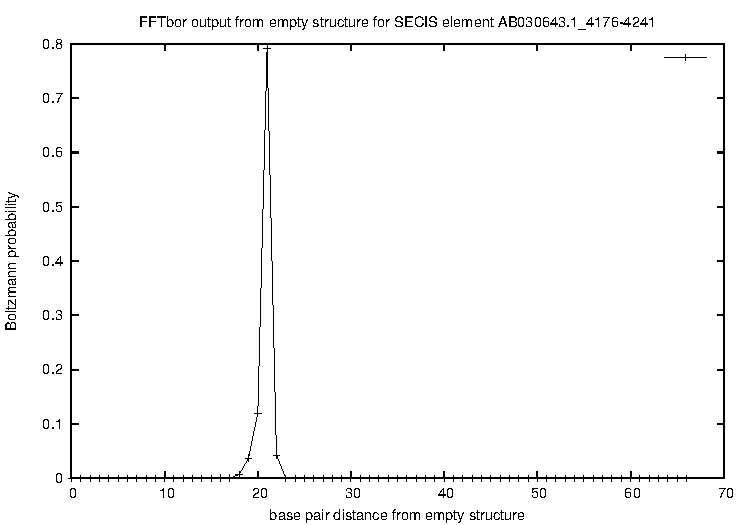
\includegraphics[width=.3\textwidth]{Figures/FFTbor/AB030643_1_4176-4241.pdf}
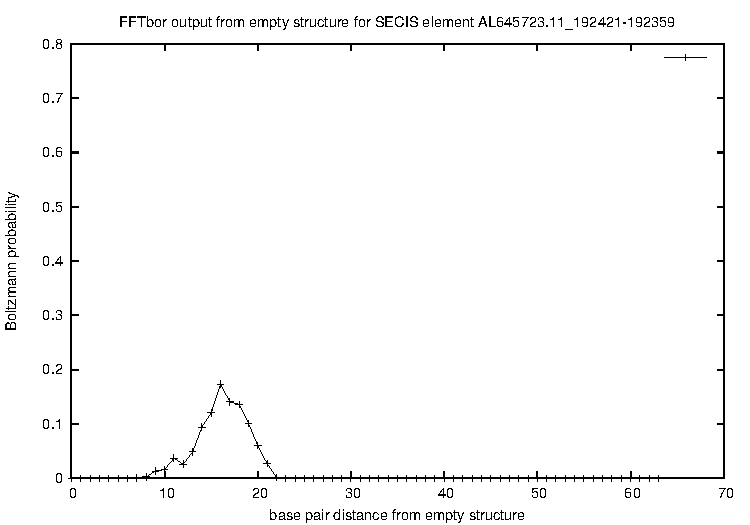
\includegraphics[width=.3\textwidth]{Figures/FFTbor/AL645723_11_192421-192359.pdf}
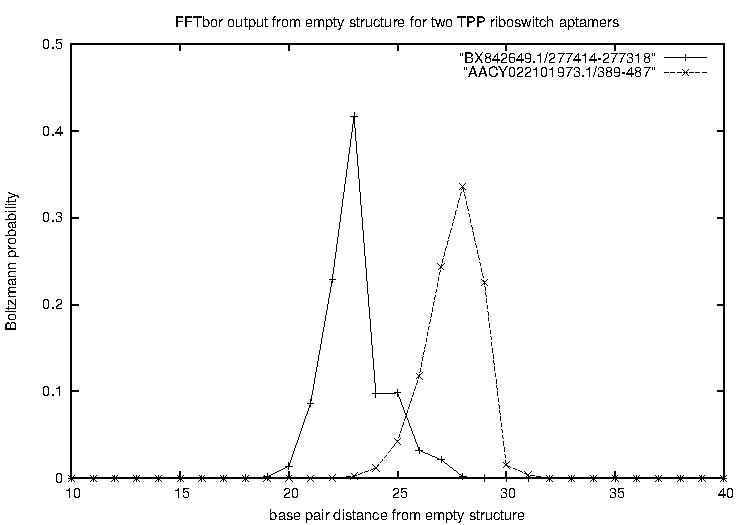
\includegraphics[width=.3\textwidth]{Figures/FFTbor/FFTborOutputFromEmptyStrForTPPriboswitches.pdf}
\caption[Example of the graphical output of \fftbor, when the empty structure is chosen as initial structure \strSt]{This figure represents the
graphical output of \fftbor, when the empty structure is chosen as
initial structure \strSt.
The $x$-axis represents the number of base pairs per structure,
taken over the ensemble of all secondary structures for the given RNA
sequence; the $y$-axis represents Boltzmann probability
$p(k) = \frac{\bfZ{k}{}}{\fullZ}$,
where \fullZ is the partition function for all secondary structures
having exactly $k$ base pairs.
{\em (Left)}
For the selenocysteine (SECIS) element AB$030643.1$ $4176$--$4241$ from Rfam family
RF$00031$, the standard deviation $\sigma$ of the number of base pairs,
taken over the ensemble of all secondary structures, is
$0.7276$, while the logarithm base $10$ of the \mfpt ($\log_{10}(\text{MFPT})$)
is $4.75$.
{\em (Center)}
For the selenocysteine (SECIS) element
AL$645723.11$ $192421$--$192359$ from Rfam family
RF$00031$, the standard deviation $\sigma$ of the number of base pairs,
taken over the ensemble of all secondary structures, is
$2.6794$, while $\log_{10}(\text{MFPT})$ is $5.69$.
Among the $61$ sequences in the seed alignment of RF$00031$,
AB$030643.1$ $4176$--$4241$ was the fastest folder, while
AL$645723.11$ $192421$--$192359$ was the slowest folder.
{\em (Right)}
Superimposition of output of \fftbor for two TPP \rb aptamers: the
$97$ nt sequence BX$842649.1$ $277414$--$277318$ and the
$99$ nt sequence AACY$022101973.1$ $389$--$487$, both obtained when
taking the empty structure for the initial structure \strSt.
The mean $\mu$ for the \fftbor structural profile near the empty
structure is $23.0203$  [resp. $27.5821$], the
standard deviation $\sigma$ for the \fftbor structural profile
is $2.2253$  [resp. $1.9857$], and the \kinfold MFPT is
$311,075.06$ [resp. $61,575.69$] for the TPP \rb aptamer
AB$030643.1$ $4176$--$4241$ [resp. AL$645723.11$ $192421$--$192359$].
The right panel of this figure should be compared with Figure
\ref{fig:fftbor:tppDistributions}.
These anecdotal results bear up the correlation between standard deviation
$\sigma$ and $\log_{10}(\text{MFPT})$ described in Table \ref{table:correlationFFTborEmpty}.
}
\label{fig:fftbor:correlationFFTborEmpty}
\end{figure}

In the right panel of \Figref{fftbor:correlationFFTborEmpty}, we
applied \fftbor to each of the two randomly chosen TPP \rb
aptamers BX$842649.1$ $277414$--$277318$ and AACY$022101973.1$ $389$--$487$, starting
from the empty reference structure $\strSt=\varnothing$.
The mean for the \fftbor structural profile near the empty
structure is $\mu_1=23.0203$  [resp. $\mu_2=27.5821$], the
standard deviation $\sigma$ for the \fftbor structural profile
is $\sigma_1=2.2253$  [resp. $\sigma_2=1.9857$], and the \kinfold MFPT is
$311,075.06$ [resp. $61,575.69$] for the TPP \rb aptamer
AB$030643.1$ $4176$--$4241$ [resp.  AL$645723.11$ $192421$--$192359$]. This anecdotal evidence supports the hypothesis that small standard deviation in \fftbor distribution is correlated with fast folding.

We randomized the TPP \rbs BX$842649.1$ $277414$--$277318$ and AACY$022101973.1$ $389$--$487$ by using our implementation of the Altschul-Erikson dinucleotide shuffle algorithm
\citep{altschulErikson:dinucleotideShuffle}, and then applied \fftbor to these
sequences, starting from the empty structure.  The mean $\mu_1$ and standard
deviation $\sigma_1$ for the \fftbor distribution for randomized BX$842649$ are
respectively $\mu_1=19.93$ and $\sigma_1=2.88$, while those for randomized
AACY$022101973$ are $\mu_2=24.39$ and $\sigma_2=24.00$. Running \kinfold, with a
maximum of $500,000$ steps with $30$ replicates (as explained in the text), we
found
that for randomized BX$842649$, all $30$ runs converged yielding a \mfpt
(MFPT) of $13,022.58$ with standard deviation of $15,221.78$. In contrast for
randomized AACY$022101973$, only $15$ out of $30$ runs converged within $500,000$ steps,
and discounting these nonconvergent data, we obtain an average \mfpt
(MFPT) of $94,446.93$ with standard deviation of $157,107.43$. This additional
test provides more anecdotal evidence supporting our hypothesis that small
standard deviation $\sigma$ in \fftbor probability density is correlated with fast folding, as measured by MFPT.

This notion of correlation between the coarse-grained energy landscape and
kinetics is what motivates the work described in Chapters \ref{ch:ffttwo}
and \ref{ch:hermes}, where a more detailed explanation of kinetics is provided,
and additional evidence is provided to support this claim.

\section{Performance characteristics of \fftbor and \rnabor}
\label{sec:fftbor:speed}

As visible from the defining recursions, the algorithmic time complexity of
\rnabor is \On{5} and space complexity is \On{3}, where $n$ is
the length of input RNA sequence. In contrast, the time complexity of
\fftbor is \On{4} and space complexity is \On{2}.
While \fftbor saves an order of magnitude in performance and memory,
\rnabor has the benefit of producing suboptimal structures $\text{MFE}_k$
for all $0 \leq k \leq n$, whose free energy is minimal across all structures
having \bpd $k$ from input structures \strSt.
\Figref{fftbor:benchmarking} displays run time curves for both
\rnabor and \fftbor, when the initial structure \strSt is
taken to be either the empty structure or the \mfe
(MFE) structure.

Here, we compare the run time of \rnabor \citep{freyhult.b07} and
the (unparallelized version of) \fftbor, using
a Dell Power Edge $1950$, $2$ x Intel Xeon E$5430$ Quad
core with $2.80$ GHz and $16$ GB RAM. For $n = 20,40,60,\dots,300$, in step
size of $20$ nt, we generated $n$ random RNA sequences of length $n$ with equal
probability for each nucleotide A,C,G,U (i.e. a 0th order Markov chain).
For values of $n \leq 200$, $100$ random sequences of length
$n$ were generated, while for values of $220 \leq n \leq 300$, only
$10$ sequences of length $n$ were generated.
RNA sequences larger than $300$ nt were not tested,
due to \On{3} memory constraints required by \rnabor.
For each RNA sequence, \rnabor and \fftbor were both run,
each starting with empty initial structure \strSt, and also
with initial sequence \strSt taken to be the MFE structure.
Each data point in the table comprises the average run time for three
independent evaluations.

\begin{figure}[!ht]
\centering
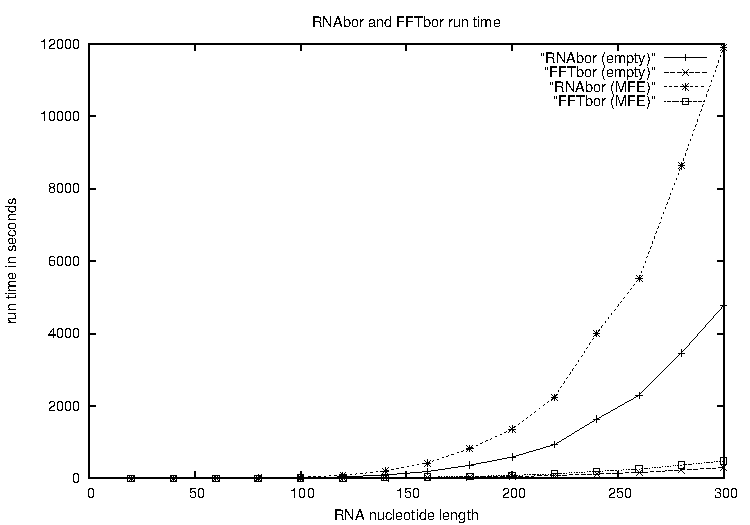
\includegraphics[width=.9\textwidth]{Figures/FFTbor/rnaborfftborRunTimeEvan.pdf}
\caption[Run times in seconds for \rnabor and \fftbor, on random RNA
of length $20$--$300$ in step size of $20$ nt]{Run times in seconds for \rnabor and \fftbor, on random RNA
of length $20,40,60,\dots,300$ in step size of $20$ nt. Each algorithm
was run with the empty initial structure \strSt, see rows
\rnabor (empty), \fftbor (empty), and with the \mfes as the initial structure
\strSt, see rows
\rnabor (MFE) and \fftbor (MFE). Note that for both \rnabor
and \fftbor, the run time increases when \strSt is the MFE structure,
rather than the empty structure. Notice the radical improvement in the
run time of \fftbor over that of \rnabor.
}
\label{fig:fftbor:benchmarking}
\end{figure}

\subsection{OpenMP parallelization of \fftbor}
\label{subsec:fftbor:openmp}

OpenMP is a simple and flexible
multi-platform shared-memory parallel programming environment, that supports
parallelizations of C/C++ code---see \url{http://openmp.org/}.
Using OpenMP primitives, we created multiple threads to evaluate the polynomial
\fullZx on different \nRoUs. \Figref{fftbor:benchmarkingParallel}
presents benchmarks, executed on
a $24$-core AMD Opteron $6172$ with $2.10$GHz and $64$GB RAM, for the speedup
of \fftbor as a function of the number of cores.
The data in Table \ref{table:fftborBenchmarkingParallel} describes average
run time in seconds ($\pm$ one standard deviation) for running \fftbor
on random RNA of length $200,250,300,400,450,500$ with either $1$ or $2$ cores.
\Figref{fftbor:benchmarkingParallel}
presents similar data for running
\fftbor on $2,3,6,4,12,15,20$ cores.

\begin{table}[!ht]
\centering
\begin{tabularx}{\linewidth}{c *{2}{R}}
\toprule
\small{$n$} & \small{Single core} & \small{Two cores} \\
\cmidrule(lr){1-3}
$200$ & $123.2 \pm 16.2$ & $61.8 \pm 8.0$ \\
$250$ & $331.1 \pm 27.2$ & $166.1 \pm 13.7$ \\
$300$ & $723.4 \pm 59.9$ & $365.2 \pm 30.1$ \\
$350$ & $1,380.8 \pm 95.2$ & $698.4 \pm 46.9$ \\
$400$ & $2,239.1 \pm 210.9$ & $1,129.5 \pm 104.3$ \\
$450$ & $3,635.0 \pm 857.4$ & $1,980.9 \pm 126.5$ \\
$500$ & $5,076.7 \pm 1,292.1$ & $3,389.8 \pm 788.4$ \\
\bottomrule
\end{tabularx}
\caption[Table showing parallel run times in seconds
for \fftbor, using OpenMP]{Table showing parallel run times in seconds
for \fftbor, using OpenMP---\url{http://openmp.org/}.
For each sequence length $200,\dots,500$,
five random RNAs were generated using equal probability for each nucleotide
A,C,G,U. Run time in seconds, plus or minus one standard deviation, are
given for a $24$-core
AMD Opteron $6172$ running at $2.10$GHz with $64$GB RAM, with only $1$ [resp. $2$] cores
used.}
\label{table:fftborBenchmarkingParallel}
\end{table}

\begin{figure}[!ht]
\centering
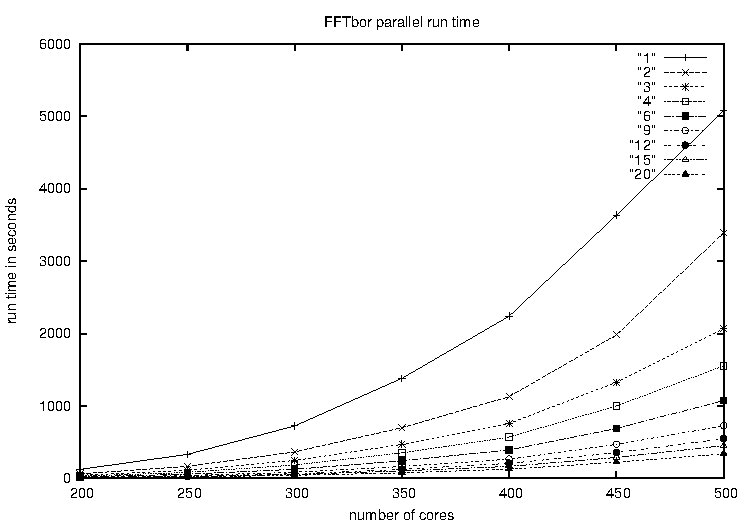
\includegraphics[width=.75\textwidth]{Figures/FFTbor/fftborParallelRunTimes.pdf}
\caption[]{Graph showing parallel run time of \fftbor as a function of
sequence length, running on an AMD Opteron $6172$ running at $2.10$GHz with $64$GB RAM,
using respectively $1,2,3,4,6,9,12,15,20$ cores.
}
\label{fig:fftbor:benchmarkingParallel}
\end{figure}

% %!TEX root = ../main.tex

\newcommand{\ob}{\,\mbox{\bf\texttt{[}}\,}
\newcommand{\cb}{\,\mbox{\bf\texttt{]}}\,}
\newcommand{\unafold}{\mbox{\tt UNAFold}\xspace}
\newcommand{\mfold}{\mbox{\tt mfold}\xspace}
\newcommand{\rnahairpinml}{\mbox{\tt RNAmloopHP}\xspace}
\newcommand{\rnamloop}{\mbox{\tt RNAmloop}\xspace}
\newcommand{\rnamlnumber}{\mbox{\tt RNAmloopNum}\xspace}
\newcommand{\rnamlorder}{\mbox{\tt RNAmloopOrder}\xspace}
\newcommand{\rnahairpin}{\mbox{\tt RNAhairpin}\xspace}
\newcommand{\rnaz}{\mbox{\tt RNAz}\xspace}

\chapter{RNAparametric} % Main chapter title

\label{RNAparametric} % Change X to a consecutive number; for referencing this chapter elsewhere, use \ref{ChapterX}

\lhead{Chapter X. \emph{RNAparametric}} % Change X to a consecutive number; this is for the header on each page - perhaps a shortened title

We describe four novel algorithms,
{\rnahairpin}, {\rnamlnumber}, {\rnamlorder}, {\rnahairpinml},
which compute
the Boltzmann partition function for global {\em structural constraints} --
respectively for the number of hairpins, the number of multiloops,
maximum order (or depth) of multiloops, and the {\em simultaneous}
number of hairpins and of multiloops.  Given an RNA sequence of length $n$
and a user-specified integer $0 \leq K \leq n$,
{\rnahairpin} [resp. {\rnamlnumber} resp. {\rnamlorder}] computes
the partition functions $Z(k)$ for each $0 \leq k \leq K$ in
time $O(K^2 n^3)$ and space $O(K n^2)$. The program {\rnahairpinml}
simultaneously computes the partition functions $Z(m,h)$ for each
possible number $m$ of multiloops and $h$ of hairpins, for
$0 \leq m \leq M$ and $0 \leq h \leq H$, with run time
$O(M^2 H^2 n^3)$ and space $O(MH n^2)$. In addition, programs
{\rnahairpin} [resp. {\rnahairpinml}] sample from the low energy
ensemble of structures having exactly $h$ hairpins [resp. $m$ multiloops
and $h$ hairpins], for user-specified values of $h,m$.
Moreover, by using the fast Fourier transform (FFT),
{\rnahairpin} and {\rnamlnumber} have been improved to run in
time $O(n^4)$ and space $O(n^2)$, although this improvement is not possible
for {\rnamlorder}.

We present two applications of the novel algorithms. First, we show that
for many Rfam families of RNA, structures sampled from {\rnahairpinml}
are more accurate than the minimum free energy structure; for instance,
sensitivity improves by almost 24\% for transfer RNA, while for
certain ribozyme families, there is an improvement of around 5\%.
Second, we show that the probabilities $p(k) = Z(k)/Z$
of forming $k$ hairpins [resp. multiloops] provide discriminating
novel features for a support vector machine or relevance vector machine
binary classifier for Rfam families of RNA.
Our data suggests that multiloop order does
not provide any significant discriminatory power over that of hairpin
and multiloop number, and since these probabilities
can be efficiently computed using the FFT, hairpin and multiloop formation
probabilities could be added to other features in existent
noncoding RNA gene finders.
Our programs, written in C/C++, are publicly available at
{\tt http://bioinformatics.bc.edu/clotelab/RNAparametric}.

\section{Introduction}

It has recently emerged that RNA plays surprising and previously unsuspected
roles in many biological processes, including retranslation of the genetic code
(selenocysteine insertion \citep{boeckForschhammer}, ribosomal frameshift
\citep{denise:frameshift}), gene regulation by allostery
(riboswitches) \citep{mandalBoeseBarrickWinklerBreaker}
and by the RISC complex (microRNAs) \citep{burgeBartel:miRNAscience},
regulation of heat shock protein expression by
temperature sensitive conformational switches \citep{ROSEswitch,tuckerBreaker:review},
pointwise editing of messenger RNA (guide RNA)
\citep{haeseler:Cryptogenes}, chemical
modification of specific nucleotides in the ribosome (small nucleolar RNAs)
\citep{loweEddy:snoRNAinArchaea},
regulation of alternative splicing \citep{Cheah.n07},
regulation of chromatin remodeling (small interfering RNAs)
\citep{Cam.c09} etc. RNA can encode
genomic information (e.g. HIV and hepatitis C) and with no assistance
from proteins can catalyze reactions such as peptidytransferase
(at ribosomal P-site) \citep{weinger:peptidyltransferase}
and cleavage
of RNA phosphodiester bonds at specific sites (group I introns)
\citep{intron:reviewCech}.
Since RNA plays various unsuspected regulatory and catalytic roles, and
since it is known from the {\sc encode} consortium report
\citep{encodeConsortium} that
the human genome is ``pervasively transcribed'',
most of whose RNA transcripts have completely unknown structure
and function, it is clear that the development of
noncoding RNA gene finders
remains an important open problem, despite significant
advances with tools such as {\rnaz} \citep{Gruber.nar07},
{\foldalign} \citep{Havgaard.nar05}, etc. The current paper
provides novel computable features that could prove useful
in enriching features sets for noncoding RNA gene finders.

In this paper, we present four novel
thermodynamics-based algorithms to compute parametric structural aspects of the
Boltzmann ensemble of low energy structures for a given RNA sequence.
Specifically, given an RNA sequence $\seq =a_1,\ldots,a_n$ and
optionally an upper bound $K$, {\rnahairpin} computes, for each value of
parameter $k$, for $0 \leq k \leq K \leq n$, the Boltzmann partition
function $Z^h(k)$ and
Boltzmann probability $p_h(k) = Z^h(k)/Z$ of all structures  of \seq having
exactly $k$ hairpins. Here $Z^h(k)$ designates the sum of Boltzmann factors
\boltzf{\str}, taken over all
secondary structures $S$ of \seq that have exactly $k$ hairpins; the
partition function $Z$ denotes the sum of all Boltzmann factors, where the
sum is taken over all secondary structures of \seq. Analogously,
{\rnamlnumber} computes, for each value of $0 \leq k \leq K \leq n$,
the Boltzmann partition function $Z^m(k)$ and probability
$p_m(k) = Z^m(k)/Z$ of all structures, that have exactly $k$
multiloops.
The program {\rnamlorder} computes the
Boltzmann partition function $Z^d(k)$ and probability
$p_d(k) = Z^d(k)/Z$ of all structures, having multiloops of order
$k$ but none of larger order, where {\em multiloop order} is
is the maximum depth of multiloop nesting.
(See Section~\ref{section:multiloopOrderPartitionFunction} for
formal definition.)
Finally, {\rnahairpinml} simultaneously computes the
Boltzmann partition function $Z(m,h)$ and probability
$p(m,h) = Z(m,h)/Z$ of all structures, having $m$ multiloops and
$h$ hairpins. Since our preliminary work showed that structures sampled
from {\rnahairpin} could improve structure prediction for certain Rfam
families, the program {\rnahairpinml} also supports sampling.

Other groups have shown an interest in global structural features
of RNA families. Here we cite four specific examples.
First, Hofacker et al.  \citep{hofacker99a} determined the asymptotic
number of hairpins, multiloops, and other structural features for
random RNA, using the homopolymer model first introduced by
Stein and Waterman \citep{steinWaterman}.
Second, Giegerich et al. \citep{giegerich:shapesBioinf} developed the
program {\tt RNAshapes}, which computes the minimum free energy structure
for various {\em shapes}; for instance, the cloverleaf shape of tRNA is
$\ob \ob \cb \ob \cb \ob \cb \cb$.
Third, the {\sc rna strand} database \citep{Andronescu.bb08}
consists of 4666 RNA secondary
structures collected from other databases, including
the Nucleic Acid Database \citep{berman03}, the Protein Data Bank
\citep{Berman.acdb02}, Sprinzl's tRNA database
\citep{sprinzl}, Gutell's database \citep{gutell:ribosomalRNA}, etc.
%(see \citep{Andronescu.bb08} for
%citation of original data sources).
{\sc rna strand} provides frequency analysis for sequence length,
number of stems, hairpin loops, bulges, internal loops, multiloops,
pseudoknots, etc., which can be generated for a
class of RNAs selected by the user from a set of predefined RNA classes,
such as 16S ribosomal RNA, 23S ribosomal RNA, 5S ribosomal RNA,
7SK RNA, ciliate telomerase RNA, cis-regulatory element, group I intron,
etc.
Fourth, Kazan et al. \citep{Kazan.pcb10} presented a machine learning
algorithm {\tt RNAcontext}, which used sequence profiles (sequence LOGOS)
as well as local secondary structure profiles (structure LOGOS) to
predict RNA nucleotides that bind to a particular riboprotein. Here,
a structural profile computes the frequency, for each $k$ in the putative
binding region,  that nucleotide position $k$ is located in a hairpin,
bulge/internal loop, multiloop, or base pair (frequencies are obtained
by counting instances from {\tt Sfold} samples).

Additionally, a number of groups have developed
algorithms to compute the minimum free energy structure and
partition function by integrating base pairing constraints.
These constraints may be {\em hard}, in the sense that
certain nucleotides are required to pair with certain other
nucleotides, while other nucleotides may be required to be unpaired.
Alternatively, constraints may be {\em soft}, in the sense that
certain nucleotides are more likely to be paired or unpaired.
Since chemical and enzymatic probing data (SHAPE, in-line probing,
PARS) is not binary 0/1, such soft constraints permit a better
mathematical integration of such footprinting data in structure
prediction. For instance, the methods of Deigan et al.  \citep{Deigan.pnas09}
and Zarringhalam et al.  \citep{Zarringhalam.po12} obtain accuracies
of $96-100\%$ for RNA structure prediction of moderate size.
See the papers of  Mathews et al.  \citep{mathewsConstraints},
Deigan et al. \citep{Deigan.pnas09},
Zarringhalam et al. \citep{Zarringhalam.po12}, and
Washietl et al. \citep{Washietl.nar12}.

Our contribution in this paper is to extend such constrained structure
prediction to more global features, such as requiring secondary structures
to have a certain number of hairpins, a certain number of multiloops and
multiloops of a certain maximum order.  In addition to computing the
number of structures having $k$ hairpins and the partition function $Z^h(k)$
for each $0 \leq k \leq K \leq n$, the program {\rnahairpin} can
additionally sample a user-specified number of low energy structures having a
user-specified number of hairpins.  Similarly, the program {\rnahairpinml}
samples low energy structures simultaneously having $m$ multiloops and
$h$ hairpins, for user-specified values of $m,h$.  In future work,
we hope to extend
{\rnamlnumber} and {\rnamlorder} to sample low energy structures having
a user-specified number or order of multiloops, and to extend all algorithms
to compute parametric minimum free energy structures -- for instance, in the
case of {\rnahairpinml}, to compute the minimum free energy structure over
all structures having $m$ multiloops and $h$ hairpins.

The following is the plan of the paper.
Section~\ref{section:definitions} introduces standard definitions and
notation to be used. Since our algorithms derive from
McCaskill's algorithm \citep{mcCaskill} to compute the partition function
$Z= \sum_{S} \exp(-E(S)/RT)$, for the benefit of the reader, we present
that algorithm in Section~\ref{section:McCaskill}.
Sections~\ref{section:hairpinPartitionFunction},
\ref{section:multiloopNumberPartitionFunction}, and
\ref{section:multiloopOrderPartitionFunction}
respectively describe the algorithms to compute the partition functions
$Z^h(k)$, $Z^m(k)$, $Z^d(k)$ for formation of $k$ hairpins
$k$ multiloops and (maximum) order $k$ multiloops, for all $k$.
Section~\ref{section:applications} describes two applications of the
new algorithms, and Section~\ref{section:discussion} presents a
discussion and conclusion of the paper. In the Appendix, we describe
how the fast Fourier transform is used to speed up the computations of
{\rnahairpin} and {\rnamlnumber}.


%Boltzmann probabilities for number of hairpins and the number/order of
%multiloops can be {\em approximated} by using {\sfold} \citep{Ding.nar04}
%to sample a large number of structures from the Boltzmann ensemble.
%Nevertheless, {\sfold} cannot approximate the {\em parametric partition
%functions} $Z^h,Z^m,Z^d$,
%computed by our software, and the frequencies computed by
%{\sfold} are not as precise as our {\em exact} method.
%For instance, by sampling 1000 structures from the low energy ensemble,
%using the command
%\begin{quote}
%{\tt RNAsubopt -d0 -p 1000}
%\end{quote}
%for the Vienna RNA Package implementation of {\sfold}, we obtain
%hairpin formation probabilities
%$p^3=0.913$, $p^4=0.087$, $p^5=0.000$, although the real probabilities
%obtained using {\rnahairpin} are
%$p^3=0.90663$, $p^4=0.09296$, $p^5=0.00040$.
%These are only slight differences, but since we are using hairpin,
%multiloop and order probabilities as features for a support vector machine,
%there is an advantage to computing the exact value.


\section{Basic definitions}
\label{section:definitions}

In this section, we introduce some notation and definitions used in the
description of the algorithms {\rnahairpin}, {\rnamlnumber} and
{\rnamlorder}.
Let $a = a_1,\ldots,a_n$ be an arbitrary
RNA sequence, and let $a[i,j]$ denote the subsequence $a_i,\ldots,a_j$.
Given an RNA sequence $a = a_1,\ldots,a_n$, a secondary structure is
a set of ordered pairs corresponding to
base pair positions, which satisfies the following requirements.
\begin{enumerate}
\item
{\em Watson-Crick or GU wobble pairs:}
If $(i,j)$ belongs to $S$, then pair $(a_i,a_j)$ must be one of the following
canonical base pairs:
$(A,U)$, $(U,A)$, $(G,C)$, $(C,G)$, $(G,U)$, $(U,G)$.
\item
{\em Threshold requirement:}
If $(i,j)$ belongs to $S$, then $j-i > \theta$.
\item
{\em Nonexistence of pseudoknots:}
If $(i,j)$ and $(k,\ell)$ belong to $S$, then it is not the case that
$i<k<j<\ell$.
\item
{\em No base triples:}
If $(i,j)$ and $(i,k)$ belong to $S$, then $j=k$;
if $(i,j)$ and $(k,j)$ belong to $S$, then $i=k$.
\end{enumerate}
Following standard convention,
the threshold $\theta$, or minimum number of unpaired
bases in a hairpin loop, is taken to be $3$.

Secondary structures are
often portrayed in {\em dot bracket notation}, consisting of a balanced
parenthesis expression with dots. Positions $i,j$ occupied by left and
right parenthesis correspond to the base pair $(i,j)$, while positions
occupied by a dot correspond to an unpaired position $i$. The dot bracket
notation for the minimum free energy (MFE) structure for
the selenocysteine insertion element {\tt fdhA} is
\begin{quote}
\begin{tiny}
\mverbatim
CGCCACCCUGCGAACCCAAUAAUAAAAUAUACAAGGGAGCAAGGUGGCG
(((((((.(((...(((.................))).))).)))))))
|mendverbatim
\end{tiny}
\end{quote}
with free energy -20.53 kcal/mol.
A {\em pseudoknot} (not considered in our software
{\rnahairpin}, {\rnamlnumber}), and {\rnamlorder}
consists of two {\em unnested} base
pairs, $(i,j)$, $(k,\ell)$, where $i<k<j<\ell$.

In defining multiloops below, we will
have recourse to the notion of {\em component}, defined as follows.
For $1 \leq i \leq \ell \leq r \leq j \leq n$, the base pair $(\ell,r)$
is an {\em exterior} base pair in the interval $[i,j]$, if there is no
base pair $(\ell',r')$ with $i \leq \ell'<\ell < r < r' \leq j$.
When the interval $i=1$ and $j=n$, then we drop mention of the interval
$[i,j]$ and simply speak of {\em exterior} base pair.
If $S$ is a secondary structure on RNA sequence $a_1,\ldots,a_n$ and
$1 \leq i\leq j \leq n$, then the number of exterior base pairs in
the interval $[i,j]$ is said to be the number of components of $S$ in $[i,j]$.

\subsubsection*{Free energy parameters}
Following the pioneering work of I.Tinoco, Jr.,
Freier et al. \citep{Freier.pnas86} measured the free energy and
enthalpy of numerous RNA hybridization duplexes, such as
$5'$-{\tt GAACGUUC}-$3'$ with its reverse complement. By least-squares
fitting, {\em base stacking} free energies were determined. By similar
methods, the Turner Lab \citep{turner,xia:RNA}
has extended and refined base stacking free energies,
loop free energies for hairpins, bulges, internal loops, multiloops, and
{\em dangles}, which latter are
stacked single-stranded nucleotides adjacent to a
{\em canonical} $5'$ or $3'$ base pair. In this paper, we use the
energy parameters from the Turner 1999 model \citep{turner,xia:RNA}
as implemented in Vienna RNA Package 1.8.5
\citep{hofacker:ViennaWebServer}, except that we do not consider
dangles. In future work, we plan to extend to the algorithms to
the Turner 2004 energy model with dangles \citep{Turner.nar09}.

\section{McCaskill's partition function}
\label{section:McCaskill}

Since our work extends McCaskill's algorithm \citep{mcCaskill}, for the
paper to be self-contained, we give a brief presentation
of McCaskill's algorithm. This presentation follows the very lucid
account given by Bompfunewerer et al.  in \citep{Bompfunewerer.jmb08}.

Given RNA nucleotide sequence $a_1,\ldots,a_n$, we will use the standard
notation $\mathcal{H}$ to denote the free energy of a hairpin,
$\mathcal{I}$ to denote the free energy of an internal loop
(combining the cases of stacked base pair, bulge and proper internal
loop), while the
free energy for a multiloop containing $N_b$ base pairs and $N_u$ unpaired
bases is given by the affine approximation $a+bN_b+cN_u$.

For RNA sequence
$a_1,\ldots,a_n$, for all $1 \leq i \leq j \leq n$, the
McCaskill partition function  $Z(i,j)$ is defined by
$\sum_S e^{-E(S)/RT}$, where
the sum is taken over all secondary structures $S$ of $a[i,j]$,
$E(S)$ is the free energy of secondary structure $S$,
$R$ is the universal gas constant with value
$R=1.987$ cal/mol$^{-1}$ K$^{-1}$, and $T$ is absolute temperature.

\begin{definition}[McCaskill's partition function]
\label{def:partitionFunctionDefMcCaskill} \hfill\break
\begin{itemize}
\item
$Z(i,j)$: partition function over all secondary structures of
   $a[i,j]$.
\item
$Z^B(i,j)$:
 partition function over all secondary structures of
   $a[i,j]$, which contain the base pair $(i,j)$.
\item
$Z^M(i,j)$:
 partition function over all secondary structures of
   $a[i,j]$, subject to the constraint that
   $a[i,j]$ is part of a multiloop and has {\em at least} one component.
\item
$Z^{M1}(i,j)$:
 partition function over all secondary structures of
  $a[i,j]$, subject to the constraint that
   $a[i,j]$ is part of a multiloop and has at {\em exactly}
   one component. Moreover, it is {\em required} that $i$ base-pair
   in the interval $[i,j]$; i.e. $(i,r)$ is a base pair, for some
   $i<r\leq j$.
\end{itemize}
\end{definition}


With this, we have the unconstrained partition function
\begin{eqnarray}
Z(i,j) &= &Z(i,j-1) + \sum_{r=i}^{j-\theta-1} Z(i,r-1) \cdot Z^B(r,j).
\end{eqnarray}
The constrained partition function closed by base pair $(i,j)$ is
given by
$Z^B(i,j)$ equals
\begin{eqnarray}
&e^{-\mathcal{H}(i,j)/RT} +
\displaystyle\sum_{i \leq \ell \leq r \leq j}
e^{-\mathcal{I}(i,\ell,r,j)/RT}\cdot Z^B(\ell,r) +\\
& e^{-(a+b)/RT} \cdot \left( \sum_{r=i+1}^{j-\theta-2} Z^M(i+1,r-1)
\cdot Z^{M1}(r,j-1) \right). \nonumber
\end{eqnarray}
The multiloop partition function with a single component and where
position $i$ is required to base-pair in the interval $[i,j]$ is given
by
\begin{eqnarray}
Z^{M1}(i,j) &= &
\displaystyle\sum_{r=i+\theta+1}^j Z^B(i,r) \cdot
e^{-c(j-r)/RT} .
\end{eqnarray}
Finally, the multiloop partition function with one or more components,
having no requirement that position $i$ base-pair in the interval $[i,j]$
is given by $Z^{M}(i,j)$ equals
\begin{eqnarray}
&
\displaystyle\sum_{r=i}^{j-\theta-1}  Z^{M1}(r,j) \cdot
e^{-(b+c(r-i))/RT}  + \\
&\displaystyle\sum_{r=i+\theta+1}^{j-\theta-1}  Z^{M}(i,r-1) \cdot
Z^{M1}(r,j) \cdot e^{-b/RT}  \nonumber
\end{eqnarray}
See \Figref{feynmanDiagram} for a pictorial representation
of the recursions of McCaskill's (original) algorithm \citep{mcCaskill};
note that the recursions are are not quite the same
as those given in \citep{hofacker:FastFolding}.
We now turn to our parametric versions of the partition function.

\begin{figure}[htp]
%\centerline{\includegraphics[width=0.6\textwidth]{feynmanDiagram}}
\centerline{\includegraphics[width=0.6\textwidth]{figure1}}
\caption{Feynman diagram of original recursions from McCaskill's
algorithm \citep{mcCaskill} to compute the partition function.
Dashed lines present intervals of unpaired bases, and shaded
arcs represent structures in which $i$ and $j$ will not necessarily pair.
}
\label{fig:feynmanDiagram}
\end{figure}
%Figure 1

%\noindent
%================ FIGURE 1 GOES ABOUT HERE ===================

\section{Hairpins}
\label{section:hairpinPartitionFunction}



We begin by defining some abbreviations for the partition function for
hairpins
\[
ZH(i,j) =
\left\{ \begin{array}{ll}
0 &\mbox{if $j-i \leq \theta$}\\
e^{-\mathcal{H}(i,j)/RT} &\mbox{else}
\end{array} \right.
\]
and internal loops having $h$ hairpins
\[
ZI^h(i,j) =  \displaystyle\sum_{i \leq k \leq \ell \leq j}
e^{-\mathcal{I}(i,j;h,k)/RT} \cdot ZB^h(k,\ell)
\]
where the sum is over $k,\ell$ such that $(k-i)+(j-\ell)>0$. This combines the
treatment of both left and right bulges with proper internal loops.

For $h\geq 0$, define the base cases $Z^h(i,i)=1$,
$ZB^h(i,i)= ZM^h(i,i)= ZM1^h(i,i)=0$.
The unconstrained partition function for secondary structures
restricted to the interval $[i,j]$ that contain $h$ hairpins is given by
\[
Z^h(i,j) =
\left\{ \begin{array}{ll}
1 &\mbox{if $h=0$}\\
Z^h(i,j-1) + \sum_{r=i}^{j-\theta-1} \sum_{h_0+h_1=h}
Z^{h_0} ZB^{h_1}(r,j) &\mbox{if $h>0$}.
\end{array} \right.
\]
The partition function for secondary structures restricted to the
interval $[i,j]$ that contain $h$ hairpins and are closed by
the base pair $(i,j)$ is given by
$ZB^h(i,j) = 0$, if $h=0$;
$ZB^h(i,j) = ZH(i,j) + ZI^h(i,j)$, if $h=1$; and for $h\geq 2$,
$ZB^h(i,j)$ is defined equal to
\[
ZI^h(i,j) + \sum_{r=i+\theta+2}^{j-\theta-2} \sum_{k=1}^{h-1}
     ZM^{k}(i+1,r-1) \cdot ZM1^{h-k}(r,j-1) \cdot e^{-(a+b)/RT}.
\]

The multiloop partition function with a single component and where
position $i$ is required to base-pair in the interval $[i,j]$ is given by
\begin{eqnarray}
ZM1^{h}(i,j) &= &
\displaystyle\sum_{r=i+\theta+1}^j ZB^h(i,r) \cdot
e^{-c(j-r)/RT} .
\end{eqnarray}
Finally, the multiloop partition function with one or more components,
having no requirement that position $i$ base-pair in the interval $[i,j]$
is given by defining $ZM^{h}(i,j)$ to equal
\begin{eqnarray}
&\displaystyle\sum_{r=i}^{j-\theta-1}  ZM1^{h}(r,j) \cdot
e^{-(b+c(r-i))/RT}  + \\
&\displaystyle\sum_{r=i+\theta+1}^{j-\theta-1} \displaystyle\sum_{k=1}^{h-1}
ZM^{k}(i,r-1) \cdot ZM1^{h-k}(r,j) \cdot e^{-b/RT}  \nonumber
\end{eqnarray}

\section{Number of multiloops}
\label{section:multiloopNumberPartitionFunction}



As before, define the abbreviations for the partition function for
hairpins
\[
ZH(i,j) =
\left\{ \begin{array}{ll}
0 &\mbox{if $j-i \leq \theta$}\\
e^{-\mathcal{H}(i,j/RT} &\mbox{else}
\end{array} \right.
\]
and internal loops having $k$ multiloops
\[
ZI^m(i,j) =  \displaystyle\sum_{i \leq k \leq \ell \leq j}
e^{-\mathcal{I}(i,j;h,k)/RT} \cdot ZB^m(k,\ell)
\]
where the sum is over $k,\ell$ such that $(k-i)+(j-\ell)>0$. As
in the previous section, this combines the
treatment of both left and right bulges with proper internal loops.

Define $Z^0(i,i)=1$, and for $m> 0$, define $Z^m(i,i)=0$. For the remaining
base cases, define $ZB^m(i,i)= ZM^m(i,i)= ZM1^m(i,i)=0$.
The unconstrained partition function for secondary structures
restricted to the interval $[i,j]$ that contain $m$ multiloops is given by
\[
Z^m(i,j) = Z^m(i,j-1)+
\sum_{r=i}^{j-\theta-1} \sum_{k=0}^m Z^k(i,r-1) \cdot ZB^{m-k}(r,j)
\]
The partition function for secondary structures restricted to the
interval $[i,j]$ that contain $m$ multiloops and are closed by
the base pair $(i,j)$ is given by
$ZB^m(i,j) = ZI^m(i,j)$, if $m=0$, and in the case that $m>0$ and
$i,j$ can form a base pair,
$ZB^m(i,j)$ equals
\begin{eqnarray*}
&ZI^m(i,j) + \displaystyle\sum_{r=i+\theta+2}^{j-\theta-2} \sum_{k=0}^{m-1}
     ZM^{k}(i+1,r-1) \\
&\cdot ZM1^{m-k-1}(r,j-1) \cdot e^{-(a+b)/RT}.
\end{eqnarray*}


The multiloop partition function with a single component and where
position $i$ is required to base-pair in the interval $[i,j]$ is given by
\begin{eqnarray}
ZM1^{m}(i,j) &= &
\displaystyle\sum_{r=i+\theta+1}^j ZB^m(i,r) \cdot
e^{-c(j-r)/RT} .
\end{eqnarray}
Finally, the multiloop partition function with one or more components,
having no requirement that position $i$ base-pair in the interval $[i,j]$
is given by $ZM^{m}(i,j)$
\begin{eqnarray}
&\displaystyle\sum_{r=i}^{j-\theta-1}  ZM1^{m}(r,j) \cdot
e^{-(b+c(r-i))/RT}  + \\
&\displaystyle\sum_{r=i+\theta+1}^{j-\theta-1} \sum_{k=1}^{m-1}
ZM^{k}(i,r-1) \cdot ZM1^{m-k-1}(r,j) \cdot e^{-b/RT}  \nonumber
\end{eqnarray}


\begin{figure}[tbhp]
\centering
%\includegraphics[scale=0.3]{haipinProfile}
%\includegraphics[scale=0.3]{MLNumber}
%\includegraphics[scale=0.3]{MLOrder}
\includegraphics[scale=0.3]{figure2a}
\includegraphics[scale=0.3]{figure2b}
\includegraphics[scale=0.3]{figure2c}
\caption{{\em (Left)}
Hairpin profile of Rfam families:
U2 spliceosomal RNA (RF00004),
transfer RNA (tRNA, RF00005) and
U4 spliceosomal RNA (RF00015).
{\em (Center)}
Multiloop number profile of
Rfam families: RNaseP (RF00010), transfer messenger RNA (tmRNA, RF00023),
and Rev response element of HIV env gene (RF00036).
{\em (Right)}
Multiloop order (or depth) profile of
Rfam families: RNaseP (RF00010), transfer messenger RNA (tmRNA, RF00023),
and Rev response element of HIV env gene (RF00036).
Notice that we chose Rfam families consisting of long RNA sequences
for multiloop number/order profiles, since multiloops are energetically
unfavorable, hence are not generally present in small RNA.
}
\label{fig:RfamProfiles}
\end{figure}
%Figure 2
%\noindent
%================ FIGURE 2 GOES ABOUT HERE ===================

\section{Multiloop order}
\label{section:multiloopOrderPartitionFunction}

%first defined
%by Waterman \citep{waterman:book} and extensively investigated by
%Nebel \citep{nebel:JCB2002},

The {\em order} (or {\em depth}) of a secondary structure is
the maximum {\em depth} of nesting of its multiloops.
Formally, multiloop order
can be defined via a finite analogue of the Cantor-Bendixson topological
derivative \citep{clote:CantorBendixson,kechris}.
The {\em derivative} $D(\strS)$ of secondary
structure $\strS$ is equal to the set of base pairs $(i,j) \in \strS$,
within which there is an internal branching; i.e.
\begin{eqnarray*}
D(\strS) &=& \{ (i,j) \in \strS : \mbox{there exist distinct
$(x,y),(u,v) \in \strS$} \\
&&\mbox{such that $i<x<y<u<v<j$} \}.
\end{eqnarray*}
The {\em order} of a secondary structure $\strS$ is now
defined to be $n-1$, where $n$ is the least integer such that
$D(\strS)=\emptyset$. For readers familiar with the notion of
RNA {\em shape} \citep{giegerich:shapesNAR},
it follows that the order of a helix is
zero, with shape $\ob \cb$, while the order of a tRNA cloverleaf secondary
structure is one, with shape $\ob \ob \cb \ob \cb \ob \cb \cb$.
Examples of order $2$ secondary structures, with shape
$\ob \ob \ob \cb \ob \cb \ob \cb \cb \ob \cb \cb$, are furnished by
certain RNase P RNA molecules, such as
{\sc strand} database \citep{Andronescu.bb08} sequence
ASE00001 from {\em Acidianus ambivalens}, and by some transfer-messenger
RNA, such as {\sc strand} database sequence
TMR00040, from {\em Azos.oryz.}.

For typographic reasons, we denote the multiloop partition function
by $Z^d$, rather than $Z^o$.
As before, define the partition function for hairpins
\[
ZH(i,j) =
\left\{ \begin{array}{ll}
0 &\mbox{if $j-i \leq \theta$}\\
e^{-\mathcal{H}(i,j)/RT} &\mbox{else}
\end{array} \right.
\]
and internal loops having multiloop order or depth $d$
\[
ZI^d(i,j) =  \displaystyle\sum_{i \leq k \leq \ell \leq j}
e^{-\mathcal{I}(i,j;k,\ell)/RT} \cdot ZB^d(k,\ell)
\]
where the sum is over $k,\ell$ such that $(k-i)+(j-\ell)>0$.
Define $Z^0(i,i)=1$ and for $d> 0$, define $Z^d(i,i)=0$.
For $d\geq 0$, define $ZB^d(i,i)= ZM^d(i,i)= ZM1^d(i,i)=0$.
The unconstrained partition function for secondary structures of multiloop
order $d$, when
restricted to the interval $[i,j]$, is given by
$Z^d(i,j)$ equals
\[
Z^d(i,j-1) + \sum_{r=i}^{j-\theta-1} \quad
    \sum_{0 \leq k,\ell \leq d, \max(k,\ell)=d}
    Z^k(i,r-1) \cdot ZB^\ell(r,j)
\]
The partition function for secondary structures of multiloop order $d$
when restricted to the
interval $[i,j]$  and are closed by
the base pair $(i,j)$ is given as follows.
For $d=0$, let
\[
ZB^d(i,j) =
ZH(i,j) + ZI^d(i,j)
\]
while for $d>0$, define
\begin{eqnarray*}
ZB^d(i,j) &=&
ZI^d(i,j) + \sum_{r=i+\theta+1}^{j-\theta-1}
    \sum_{0 \leq k,\ell \leq d, \max(k,\ell)=d} \\
&&    ZM^k(i,r-1)  \cdot
ZM1^\ell(r,j)  \cdot e^{-(a+b)/RT}.
\end{eqnarray*}


The multiloop partition function with a single component and where
position $i$ is required to base-pair in the interval $[i,j]$ is given by
\begin{eqnarray}
ZM1^{d}(i,j) &= &
\displaystyle\sum_{r=i+\theta+1}^j ZB^d(i,r) \cdot
e^{-c(j-r)/RT}.
\end{eqnarray}
Finally, the multiloop partition function with one or more components,
having no requirement that position $i$ base-pair in the interval $[i,j]$
is given by
\begin{eqnarray}
ZM^{d}(i,j) &=&
%\displaystyle\sum_{r=i}^{j-\theta-1}  ZM1^{d}(r,j) \cdot
\sum_{r=i}^{j-\theta-1}  ZM1^{d}(r,j) \cdot
e^{-(b+c(r-i))/RT}  + \\
&& \sum_{r=i+\theta+1}^{j-\theta-1}
  \sum_{0 \leq k,\ell \leq d, \max(k,\ell)=d} ZM^{k}(i,r-1) \cdot
\nonumber\\
&&ZM1^{\ell}(r,j) \cdot e^{-b/RT}.  \nonumber
\end{eqnarray}

\section{Simultaneous multiloop number and hairpin number}
\label{section:RNAhairpinml}

Given the algorithms described in Sections
\ref{section:hairpinPartitionFunction} and
\ref{section:multiloopNumberPartitionFunction}, it is straightforward
to design the algorithm {\rnahairpinml}, which computes the partitiion
function $Z(m,h)$ simultaneously for $m$ multiloops and $h$ hairpins.
Sampling low energy structures is done by a straightforward variation of
the sampling method introduced by Ding and Lawrence \citep{Ding.nar03}.
For purposes of brevity, further details of the partition function and
sampling will not be discussed, though the interested reader can study
our publicly available source code.

\section{Applications}
\label{section:applications}

In this section, we mention two main applications of the new algorithms,
though first we mention that {\rnahairpin} presents a novel method to
generate suboptimal secondary structures.


In the literature, there are a number of approaches to compute
{\em suboptimal} secondary structures. Historically, the first
method was due to Zuker \citep{Zuk89a}, as implemented in {\tt mfold}
{\tt mfold} \citep{Zuk89a} and {\tt Unafold} \citep{Markham.mmb08},
who for certain base pairs $(i,j)$ computed the minimum
free erergy structure containing $(i,j)$ that was sufficiently distinct
from previously generated suboptimal structures.
Next, the program \rnasub of Wuchty et al.
\citep{wuchtyFontanaHofackerSchuster} generated all secondary structures
within a user-specified energy above the minimum free energy.
In contrast the program {\tt Sfold} \citep{Ding.nar03} samples from
the low energy Boltzmann ensemble of structures; indeed, our implementation
of sampling in {\rnahairpin} is a modification of the method of
Ding and Lawrence \citep{Ding.nar03}. (Note that the {\tt Sfold} algorithm
is implemented in the Vienna RNA Package program
\rnasub with flag {\tt -p}; as well the program
{\tt RNAstructure} \citep{mathewsConstraints} also supports sampling.)
The program {\tt RNAshapes} of Steffen et al.
\citep{giegerich:shapesBioinf} computes the minimum free energy structure
from each shape class.
The program \rnabor of Freyhult et al. \citep{freyhult.b07}
computes, for each $k$,
the minimum free energy structure $MFE(k)$ having base pair
distance $k$ from a user-specified reference structure, while the
program \rnatwofold of Lorenz et al. \citep{hofacker:RNAbor2D}
computes, for each $k,\ell$, the minimum free energy structure
$MFE(k,\ell)$ having base pair
distance $k$ [resp. $\ell$] from a first [resp. second]
user-specified reference structure.
The program {\tt RNAlocopt} of Lorenz and Clote  \citep{RNAlocopt}
samples low  locally optimal secondary structures, where a locally
optimal structure has the property that its free energy cannot be lowered
by the addition or removal of a single base pair. The program
{\tt RNAbormea} of Lou and Clote \citep{Clote.bb12} determines
for each $k$, the maximum expected accuracy structure among all structures
having base pair distance $k$ from a user-specified reference structure.
To this list of previous methods, {\rnahairpin} generates suboptimal
secondary structures in a manner that seems orthogonal to previous methods.

\subsection{Improved structure prediction for certain RNA families}


Certain RNAs have a characteristic structure that is important for
their function. For instance, the cloverleaf structure of transfer RNA
generally has three hairpins,  which then form an L-shaped tertiary
structure by additional pseudoknots. Transfer RNAs usually contain
a small number of chemically modified nucleotides, making their structure
at times difficult to predict using minimum free energy structure methods.
In such cases, {\rnahairpin} [resp. and expecially {\rnahairpinml}]
can improve structure prediction by
sampling low energy structures that are required to have a specific
number of hairpins [resp. number $m$ of multiloops and $h$ of hairpins].

\begin{table*}[!t]
\begin{tabular}{|l|rrrrr|}
\hline
RNA family & H & {\tt RNAhairpin} $\mu \pm \sigma$ & {\tt RNAfold}
$\mu \pm \sigma$ & avg len & num seq\\
\hline
RF00001 & 2 & $0.6213 \pm 0.2667$ & $0.6332 \pm 0.2721$ & 116.6 & 712\\
RF00004 & 5 & $0.7548 \pm 0.1840$ & $0.7104 \pm 0.2058$ & 190.5 & 208 \\
RF00005 & 3 & $0.7345 \pm 0.2313$ & $0.5370 \pm 0.1992$ & 73.4 &960  \\
RF00008 & 2 & $0.9565 \pm 0.1284$ & $0.9154 \pm 0.1894$ & 55.4 & 84\\
RF00031 & 1 & $0.7679 \pm 0.1748$ & $0.7657 \pm 0.1945$ & 64.5 & 61\\
RF00045 & 4 & $0.4420 \pm 0.2983$ & $0.4205 \pm 0.3274$ & 202.6 & 66 \\
RF00094 & 2 & $0.3080 \pm 0.2131$ & $0.3604 \pm 0.2091$ & 91.1 & 33\\
RF00167 & 2 & $0.8113 \pm 0.2301$ & $0.8568 \pm 0.2290$ & 100.8 & 133 \\
RF00375 & 2 & $0.8278 \pm 0.3060$ & $0.8814 \pm 0.2044$ & 99.0 & 130\\
RF00504 & 2 & $0.5940 \pm 0.2711$ & $0.5603 \pm 0.2895$ & 100.9 & 44\\
RF00635 & 4 & $0.3024 \pm 0.1127$ & $0.3707 \pm 0.1204$ & 117.9 & 13\\
RF01055 & 4 & $0.5821 \pm 0.2725$ & $0.5787 \pm 0.2641$ & 142.0 & 160 \\
\hline
\end{tabular}
\caption{Comparison between {\tt RNAhairpin} and {\tt RNAfold}
of the average sensitivity (ratio of
number of correctly predicted base pairs in Rfam structure over
number of base pairs in Rfam structure) for various Rfam families.
{\rnahairpin}
was used to sample a single secondary structure having H many hairpins,
and the average sensitivity of {\rnahairpin} and {\tt RNAfold}
was computed over all sequences in the seed alignment of the following
Rfam families:
RF00001 (5S rRNA),
RF00004 (splicesomal U2 RNA),
RF00005 (tRNA),
RF00008 (type III hammerhead ribozyme),
RF00031 (selenocysteine insertion sequence I),
RF00045 (snoRNA),
RF00094 (HDV ribozyme),
RF00167 (purine riboswitch),
RF00375 (HIV primer binding site),
RF00504 (glycine riboswitch),
RF00635 (HAR1A),
RF01055 (moco RNA motif).
}
\label{table:sensitivity}
\end{table*}

\begin{table*}[!b]
\begin{tabular}{|l|rrrrrr|}
\hline
RNA family & M & H & {\tt RNAhairpin} $\mu \pm \sigma$ & {\tt RNAfold}
$\mu \pm \sigma$ & avg len & num seq\\
\hline
RF00001 & 1 & 2 & $0.6308 \pm 0.2571$ & $0.6332 \pm 0.2721$ & 116.6 & 712\\
RF00004 & 0 & 5 & $0.6980 \pm 0.1780$ & $0.7104 \pm 0.2058$ & 190.5 & 208 \\
RF00005 & 1 & 3 & $0.7740 \pm 0.1946$ & $0.5370 \pm 0.1992$ & 73.4 &960  \\
RF00008 & 1 & 2 & $0.9582 \pm 0.1005 $ & $0.9154 \pm 0.1894$ & 55.4 & 84\\
RF00031 & 0 & 1 & $0.7679 \pm 0.1748$ & $0.7657 \pm 0.1945$ & 64.5 & 61\\
RF00045 & 1 & 4 & $0.4456 \pm 0.2977$ & $0.4205 \pm 0.3274$ & 202.6 & 66 \\
RF00094 & 0 & 2 & $0.3464 \pm 0.1951$ & $0.3604 \pm 0.2091$ & 91.1 & 33\\
RF00167 & 1 & 2 & $0.8511 \pm 0.1726$ & $0.8568 \pm 0.2290$ & 100.8 & 133 \\
RF00375 & 1 & 2 & $0.8283 \pm 0.3063$ & $0.8814 \pm 0.2044$ & 99.0 & 130\\
RF00504 & 1 & 2 & $0.6101 \pm 0.264$ & $0.5603 \pm 0.2895$ & 100.9 & 44\\
RF00635 & 1 & 3 & $0.2930 \pm 0.1059$ & $0.3707 \pm 0.1204$ & 117.9 & 13\\
RF01055 & 1 & 4 & $0.60170 \pm 0.277$ & $0.5787 \pm 0.2641$ & 142.0 & 160 \\
\hline
\end{tabular}
\caption{Comparison between {\rnahairpinml} and {\tt RNAfold}
of the average sensitivity for the same Rfam families, as in
Table~\ref{table:sensitivity}. By now sampling a single secondary structure
having simultaneously M many multiloops and H many hairpins, the
average sensitivity improved over that of {\rnahairpin}
in essentially all cases.
%Improvement over {\rnahairpin}: over 2\% in RF00005 (tRNA),
%4\% in RF00094 (HDV ribozyme),
%over 4\% in RF00167 (purine riboswitch),
%about 1.5\% in RF00504  (glycine riboswitch),
%about 2\% in RF01055 (moco RNA motif).
Moreover, {\rnahairpinml} provides more accurate structure
prediction (sensitivity) than {\tt RNAfold} for a number of
Rfam families. There is an improvement
of almost $approx 24\%$ in RF00005 (tRNA),
over $4\%$ in RF00008 (type III hammerhead ribozyme),
$2.5\%$ in RF00045 (snoRNA),
$5\%$ in RF00504  (glycine riboswitch),
over $2\%$ in RF01055 (moco RNA motif).
On the other hand, {\rnahairpinml} has significantly lower
sensitivity than {\tt RNAfold} in the following two cases, where
the difference is over $5\%$ for RF00375 (HIV primer binding site),
and $8\%$ for RF00635 (HAR1A).
Insignificant differences, such as
$0.6308$ for {\rnahairpinml} versus $0.6332$ in RF00001 (5S rRNA)
are likely to be due to the stochastic nature of sampling low energy
structures, rather than computing the MFE structure having a specified
number of multiloops and hairpins.
}
\label{table:sensitivityMultiloopHairpin}
\end{table*}

Table~\ref{table:sensitivity} presents a comparison of {\rnahairpin}
and {\tt RNAfold} statistics for sequences taken from the seed alignments
of several families from Rfam 11.0 \citep{Burge.nar13}
(August 2012, 2208 families).  For each sequence,
we sampled only one low energy structure having H hairpins. For a given
sequence and structure computed either by {\rnahairpin} or {\tt RNAfold},
the sensitivity, or true positive rate, is computed, defined as
the ratio of number of correctly predicted base pairs in the
Rfam structure over the number of base pairs in the Rfam structure.
The average and standard deviation of sensitivity is given, for each
Rfam family of the table, for both {\rnahairpin} and {\tt RNAstructure}.
For these computations, version 1.8.5 of {\tt RNAfold} was used without
dangles, so that both {\rnahairpin} and {\tt RNAfold} employed the same
energy model. In future work, we plan to lift {\rnahairpin} to
the Turner 2004 energy model and implement dangles, which then would
support the same energy model as version 2.0 and higher of
{\tt RNAfold} \citep{Lorenz.amb11}.


In the case of tRNA, there is more than 20\% improvement in sensitivity
of {\rnahairpin} over {\tt RNAfold}; {\rnahairpin} has greater sensitivity
than {\tt RNAfold} for other instances, such as
in the case of the hammerhead ribozyme (around 4\% improvement).
On the other hand, {\tt RNAfold} has greater
sensitivity than {\rnahairpin} for several classes, including
HIV primer binding site RF00375 (over 5\% improvement), and
purine riboswitch aptamers RF00167 (around 4.5\% improvement).
Clearly {\rnahairpin} is not a better structure prediction tool than
{\tt RNAfold}; however, for particular classes of functional RNA,
which require certain hairpin structures for function, {\rnahairpin}
may provide a useful tool. See Section~\ref{section:discussion} for
more discussion.

The program {\rnahairpinml}, which samples low energy structures having
$m$ multiloops and $h$ hairpins,  improves the structure prediction
accuracy of {\rnahairpin} (e.g. an improvement of over 4\% for RF000167
purine riboswitches), and also outperforms {\tt RNAfold} for a larger number
of cases on the previously described Rfam families. For instance,
there is an improvement
of almost $approx 24\%$ in RF00005 (tRNA),
over $4\%$ in RF00008 (type III hammerhead ribozyme),
$5\%$ in RF00504  (glycine riboswitch), etc.
On the other hand, {\rnahairpinml} has significantly lower
sensitivity than {\tt RNAfold} in the following two cases, where
the difference is over $5\%$ for RF00375 (HIV primer binding site),
and $8\%$ for RF00635 (HAR1A). The consensus structures for these
Rfam families have large loop regions, which may in fact be base-paired,
which could explain the poorer performance of {\rnahairpinml}.
(Recall that Rfam consensus structures are determined by covariation found
in multiple alignments, thus loop regions in consensus structures could
indeed by base-paired and involve additional hairpins and/or multiloops.)
In any case, we do not propose the use of {\rnahairpinml} in place of
minimum free energy structure software, such as {\tt RNAfold}; instead,
if a biologist has knowledge or intuition about the existence of a certain
number of multiloops and hairpins, then {\rnahairpinml} may prove to be a
useful tool.

\begin{table*}
\begin{tabular}{|l|rrrrrr|}
\hline
Family name and description & H & HM & HMO & num seq& avg len & avg GC \% \\
\hline
RF00004 U2 spliceosomal RNA & 0.9217  & 0.9282  & 0.9328  & 208 & 204.26 &48.0\% \\
RF00005 tRNA &  0.6367  & 0.9038  & 0.9017  & 959 & 73.4& 47.0\%\\
RF00008 hammerhead III &  0.9191  & 0.9705  & 0.9562  & 84 & 55.4 & 48.4\% \\
RF00027 let 7 microRNA precursor &  0.8338  & 0.8766  & 0.8617  & 67 & 79.6 & 43.7\% \\
RF00031 SECIS 1 & 0.7917  & 0.8361  & 0.7941  & 61 & 64.5 & 49.0\% \\
RF00045 SNORA73 & 0.6306  & 0.6515  & 0.6609  & 66 & 202.6 & 53.1\% \\
RF00167 purine riboswitch & 0.6508  & 0.8608  & 0.8529  & 136 & 100.8 & 38.1\% \\
\hline
\end{tabular}
\caption{Area under curve (AUC) for receiver operating characteristic
(ROC) curves for
seven Rfam families, each family tested under 5-fold cross-validation with
support vector machines (SVM) using a radial basis kernel with
cost $C=1$ and $\gamma$ equal to the inverse of the number of features.
In the case of H (hairpin number), there were 21 hairpin formation
probabilities $p(0),\ldots,p(20)$ taken as features,
(though in
most cases all but a very small number of these probabilities were zero);
in the case  of HM (hairpin and multiloop number), there were
27=21+6 hairpin and multiloop formation probabilities taken as
features, and in the case  of HMO
(hairpin and multiloop number with maximum multiloop order), there were
27=21+6 hairpin and multiloop formation probabilities taken as features
along with 6 multiloop maximum order probabilities, hence altogether
33=21+6+6 features.
The R packages {\tt e1071} \citep{RpackageForSVM} and {\tt pROC} \citep{pROC}
were used with {\tt libSVM} \citep{libSVM}.
}
\label{table:AUC}
\end{table*}

\begin{table*}
\begin{tabular}{|l|rrrrrrr|}
\hline
Ratio SVM/RVM &RF00004& RF00005& RF00008& RF00027& RF00031& RF00045& RF00167\\
\hline
HP&      0.9874&  1.0657&  0.9874&  1.4234&  1.1965&  0.9895&  1.1894\\
HP/M&    0.9863&  0.9798&  0.9977&  1.0625&  1.0954&  0.9808&  1.0153\\
HP/M/O&  0.9818&  0.9855&  1.0025&  0.8986&  1.2324&  1.0237&  1.0031\\
\hline
\end{tabular}
\caption{Ratio of ROC area under curve values for two types of machine
learning methods: support vector machines (SVM) and relevance vector
machines (RVM), using the same seven Rfam families that were considered
in Table~\ref{table:AUC}. In 11 out of 21 tests, AUC values for SVMs
were greater than those for RVMs. In the case of RF00027, it is interesting
to note that when using only hairpin features, SVM AUC was much higher than
RVM AUC (SVM/RVM $1.4234$), while for the same class, when using the larger
feature set for hairpins, multiloop number and multiloop order, SVM AUC
was lower than RVM AUC (SVM/RVM $0.8986$). At present, the reason for
this surprising result is unclear.
The R packages {\tt e1071} \citep{RpackageForSVM} and {\tt pROC} \citep{pROC}
were used for SVM and RVM computations;
for SVM, the radial basis kernel (rbfkernel) was employed with
default parameters, while for RVM, rvmbinary
rbfdot kernel was used with default parameters and 1000 iterations.
}
\label{table:RF00027aucSVMversusRVM}
\end{table*}

\subsection{Support vector machine results}

In this section, we describe receiver operating characteristic
(ROC) curves, computed by 5-fold cross-validation, where in each
case, the positive instances were taken to be sequences from the
seed alignment of a given Rfam family, and negative instances were
taken to be random sequences having the same number of dinucleotides,
as computed by our implementation of the Altschul-Erikson algorithm
\citep{altschulErikson:dinucleotideShuffle}.
(Similar results were obtained, when we took negative instances to be
sequences the seed alignments of all other Rfam families -- data not
shown.)

For each positive instance, we generated 10 random negative instances.
Using {\tt libSVM} \citep{libSVM}, we performed a {\em stratified training}
by selecting one-fifth of the
positive instances together with an equal number of negative instances
(one of the 10 negative instances was selected for each positive instance)
for training. The remaining four-fifths of the positive sequences, together
with all corresponding negative instances, constituted the test set
(note that in testing, there were 10 negative instances per positive sequence).
A radial basis kernel was chosen with cost $C=1$, and parameter $\gamma$
taken to be the reciprocal of the number of features.

We considered three features sets: HP, HP/M, and HP/M/O,
where HP features were the 21 probabilities of hairpin formation
$p_h(0),\ldots,p_h(20)$, where M features were the 6 probabilities of
multiloop formation $p_m(0),\ldots,p_m(6)$, and where O features
were the 6 probabilities of multiloop order (or depth) $p_d(0),\ldots,p_d(6)$.
Thus the SVM binary classifier HP (hairpins) has 21 features, though in
most cases all but a small number of the features are $0$;
the classifier HP/M (hairpin and multiloop number) has
27=21+6 features; the classifier HP/M/O (hairpin, multiloop number,
multiloop order) has 33=21+6+6 features.
The R packages {\tt e1071} \citep{RpackageForSVM} and {\tt pROC} \citep{pROC}
were used with {\tt libSVM} \citep{libSVM}.

Table~\ref{table:AUC} summarizes the area under curve (AUC) values for
ROC curves for the three different SVM classifiers HP, HP/M, HP/M/O,
while \Figref{SVMforU2andPurineRiboswitch} depicts the corresponding
ROC curves. Note that in all cases, inclusion of multiloop order probabilities
as features does not add any discriminatory power, and even in certain cases
reduces the AUC. This is fortunate, since {\rnamlorder} cannot be
sped up by using the fast Fourier transform, unlike {\rnahairpin} and
{\rnamlnumber}. The results of this table and figure indicate that,
although hairpin and multiloop formation probabilities may not be
sufficient to be used solely as the feature set of a noncoding RNA gene
finder, we believe that, when added, these features could lead to improvements
in performance of existent RNA gene finders. Moreover, to the best of our
knowledge, current noncoding RNA gene finders do not take into account
global propensity to form hairpins or multiloops.

Table~\ref{table:RF00027aucSVMversusRVM} presents the ratio of ROC  area
under curve values for support vector machines (SVM) over that for relevance
vector machines (RVM). A value greater [resp. less] than unity in the
table indicates that SVM outperforms [resp. underperforms] RVM using the
same features.
\Figref{RF00027aucSVMversusRVM} shows an unexpected situation
for the 5-fold (stratified) cross-validation experiments of the Rfam family
RF00027, Using the feature set consisting of only 21 hairpin
formation probabilities $p_h(0),\ldots,p_h(20)$, the ratio of SVM/RVM AUC
is $1.4234$, indicating that SVM far outperforms RVM for this family using these
features, while for the full feature set of hairpin formation probabilities
$p_h(0),\ldots,p_h(20)$, multiloop number probabilities $p_h(0),\ldots,p_h(6)$,
and multiloop maximum order (depth) probabilities $p_h(0),\ldots,p_h(6)$,
the ratio of SVM/RVM AUC is $0.8986$,
indicating that RVM outperforms SVM.


\begin{figure*}[tbhp]
\centering
%\includegraphics[width=0.45 \textwidth]{svm_rf00004_roc_curve_overlay}
\includegraphics[width=0.45 \textwidth]{figure3a}
\hskip 1cm
%\includegraphics[width=0.45 \textwidth]{svm_rf00167_roc_curve_overlay}
\includegraphics[width=0.45 \textwidth]{figure3b}
\caption{
Receiver operating characteristic (ROC) curves for the performance of
support vector machine binary classification using a
feature set consisting of probabilities
$p(0),\ldots,p(20)$ for the number hairpins (HP),
probabilities $p(0),\ldots,p(5)$ for the
number of multiloops (M), and
probabilities $p(0),\ldots,p(5)$ for the
maximum order of multiloops (O).
In the case of HP (hairpin number), there were 21 features, though in
most cases all but at most 6-8 features had the value $0$;
in the case  of HP/M (hairpin and multiloop number), there were
27=21+6 features, and in the case  of HP/M/O
(hairpin and multiloop number with maximum multiloop order), there were
33=21+6+6 features.
The R packages {\tt e1071} \citep{RpackageForSVM} and {\tt pROC} \citep{pROC}
were used with {\tt libSVM} \citep{libSVM}. A radial basis kernel was used
in each case with cost $C=1$; parameter $\gamma$ was taken to be the
inverse of the number of features, i.e. for
HP, $\gamma = 1/21 = 0.0476$, for HP/M, $\gamma = 1/27 = 0.0370$, for
HP/M/O, $\gamma = 1/33 = 0.0303$.
%
As shown in this figure, accounting for multiloop
order did not improve classification ROC curves, and data presented in
Table~\ref{table:AUC} shows that in some cases, ROC area under curve
is lessened by taking into account maximum multiloop order. This is
in fact fortunate, since the fast Fourier transform can be applied to
reduce time and space requirements for {\rnahairpin} and
{\rnamlnumber}, but not {\rnamlorder}.
{\em (Left)}
Rfam family RF00008 (U2 spliceosomal RNA).
{\em (Right)}
Rfam family RF00167 (purine riboswitch).
}
\label{fig:SVMforU2andPurineRiboswitch}
\end{figure*}

\begin{figure*}[tbhp]
\centering
%\includegraphics[width=0.45 \textwidth]{roc_rf00027_h_roc_curve_overlay}
\includegraphics[width=0.45 \textwidth]{figure4a}
\hskip 1cm
%\includegraphics[width=0.45 \textwidth]{roc_rf00027_hmo_roc_curve_overlay}
\includegraphics[width=0.45 \textwidth]{figure4b}
\caption{Receiver operating characteristic (ROC) curves for
5-fold cross-validation for sequences from the seed alignment of
RF00027.
The left panel shows an overlay of support vector machine (SVM) and
relevance vector machine (RVM) for the feature set consisting of
21 hairpin formation probabilities $p_h(0),\ldots,p_h(20)$,
while the right panel presents an overlay of SVM and RVM for the
full feature set of hairpin formation probabilities $p_h(0),\ldots,p_h(20)$,
multiloop number probabilities $p_h(0),\ldots,p_h(6)$, and
multiloop maximum order (depth) probabilities $p_h(0),\ldots,p_h(6)$.
As explained in the caption of Table~\ref{table:RF00027aucSVMversusRVM},
it seems unusual that SVM outperforms RVM using only hairpin probability
features, while the reverse is true when using the full feature set.
}
\label{fig:RF00027aucSVMversusRVM}
\end{figure*}


\section{Discussion and conclusion}
\label{section:discussion}

We terminate the paper with a discussion of strengths and shortcomings
of each application shown: improved structure prediction and
support vector machine classification.

\subsection*{Parametric structure prediction}

For benchmarking purposes in Table~\ref{table:sensitivity}, we
sampled only one low energy structure having H many hairpins, where
in most cases H was taken to be the number of hairpins in the Rfam
consensus structure of the first member of the Rfam family. This explains
how it could happen that the {\rnahairpin} sensitivity for a certain
sequence could at times be different than the {\tt RNAhairpin} sensitivity
for the same sequence, even when the sampled structure and the minimum
free energy structure have the same number of hairpins.
Of course, in general, our code {\tt RNAhairpin} will be used to
sample a large number (1,000 or 10,000) of structures per
sequence.

Since the base pairs that appear in Rfam consensus structures are
inferred by covariation observed in a multiple alignment,
many valid base pairs do not appear in the consensus structure. For
this reason, we did not compute {\em positive predictive rate}, defined
as the ratio of the number of correctly predicted base pairs in the
Rfam consensus structure, divided by the number of base pairs in the
predicted structure. This is the reason that Table~\ref{table:sensitivity}
only reports average sensitivity values.

As previously mentioned, we computed the average sensitivity of
the minimum free energy (MFE) structure obtained from Vienna RNA
Package {\tt RNAfold} \citep{hofacker:ViennaWebServer}, version 1.8.5
without dangles, in order to ensure that both {\rnahairpin} and {\tt RNAfold}
employ the same energy model.  In future work, we plan
to extend {\tt RNAhairpin} to the Turner 2004 energy model with dangles
\citep{Turner.nar09}. By the same token, it is not conceptually difficult
to modify the program {\rnamlnumber}, in order to sample low energy structures
having a specified number of multiloops. Such sampled structures could
yield better structure predictions for certain types of RNA. Finally,
it would be possible to combine the algorithms {\rnahairpin} and {\rnamlnumber}
in order sample structures having {\em both} a specified number of hairpins
and a possibly distinct number of multiloops. Nevertheless, such an
algorithm would run in time $O(H^2 M^2 n^3)$ and space $O(H M n^2)$,
where $H$ [resp. $M$] is an upper bound on the number of hairpins
[resp. multiloops]. For relatively small values of $H,M$, such an
algorithm would indeed be feasible, and could prove useful for certain
classes of RNA, whose function is known to depend on certain structural
motifs.

Table~\ref{table:sensitivity} presents examples of Rfam families, where
the average sensitivity of {\tt RNAhairpin} exceeds that of {\tt RNAfold}.
Improvements were obtained for RNA families, where a certain number of
hairpins are known to be functionally important, as in the cloverleaf
tRNA, typically having three hairpins. In this case, the sensitivity of
{\tt RNAhairpin} exceeds that of {\tt RNAfold} by approximately 20\%.
For certain ribozymes, such as type III hammerhead ribozyme (RF00008)
and glycine ribozyme (RF00504), the improvement was over 4\% resp. 3\%.
Not shown in the table are RNA families, where the sensitivity of
{\tt RNAfold} exceeded that of {\tt RNAhairpin} -- for instance,
for 5S rRNA (RF00001), {\tt RNAhairpin} average sensitivity was
$0.621306$ compared with {\tt RNAfold} sensitivity of $0.633189$;
for purine riboswitches (RF00167), {\tt RNAhairpin} obtained had
$0.811327$ compared with {\tt RNAfold} sensitivity of  $0.856764$.
We believe that {\rnahairpin} showed better sensitivity than {\tt RNAfold}
in the case of tRNA, because of two reasons: (1) tRNA has a well-known
cloverleaf structure usually involving 3 hairpins, and (2) there may
be a large sequence and energy difference among especially bacterial
tRNAs. Item (2) could cause minimum free energy structures to be quite
distinct from the usual cloverleaf -- manual investigation
confirms this hypothesis in some randomly chosen instances, while item
(2) ensures that {\rnahairpin} will sample structures having 3 hairpins,
hence more likely to adopt the functional cloverleaf structure.
It could be that similar reasons explain the small improvement of
{\rnahairpin} over {\tt RNAfold} for some of the other examples, including
certain ribozymes. However, along this line of reasoning, we expected
{\rnahairpin} to outperform {\tt RNAfold} for purine riboswitch aptamers,
which have a very well-defined multiloop with two hairpins;
Table~\ref{table:sensitivity} shows this is not the case.
As described in the caption of
Table~\ref{table:sensitivityMultiloopHairpin}, by sampling low energy
structures that simultaneously have a specified number $m$ of multiloops and
number $h$ of hairpins, we substantially improve the prediction accuracy
of {\tt RNAfold}. However, such improvements tend to occur when the Rfam
families show a prounounced common fold, as in the case of tRNA and certain
ribozymes, and when there are no large loop (undefined) regions in the
Rfam consensus structures.  In any case, we believe that
minimum free energy structure prediction algorithms, such as
{\tt RNAfold}, {\unafold}, {\mfold}, {\tt RNAstructure}, remain
the best universal thermodynamics-based tool for structure prediction.


\subsection*{Features for SVM classifiers}

The development of noncoding RNA gene finders is important for the
analysis and classification of the pervasively transcribed
RNA from the human genome, most of which has no previously known
structure or function.  In this paper, we have described
four novel thermodynamics-based algorithms, {\rnahairpin},
{\rnamlnumber}, {\rnamlorder}, and {\rnahairpinml} which
compute global, parametric features of the ensemble
of low energy secondary structures for a
given RNA sequence. For the first three algorithms, we have
shown that there is a significant {\em global} signal, as witnessed
by ROC area under curve, that suggests that probability and multiloop
formation probabilities present useful features that could be added
to existent noncoding RNA gene finders -- note that this remark only
concerns gene finders for specific noncoding RNA families, not general
ncRNA gene finders.\footnote{Since we only recently implemented
{\rnahairpinml}, we have not evaluated whether ROC AUC is better than
for {\rnahairpin} alone, or for {\rnahairpin} combined with {\rnamlnumber}.}

One of our goals in developing these parametric algorithms
was to provide additional discriminatory features that
can be added to other features within the context of
a support vector machine, in order to improve the accuracy of
noncoding RNA gene finders. Indeed, by adding novel features,
it is known that one can improve the accuracy of SVM classifiers.
For instance, the state-of-the-art precursor
microRNA (pre-miRNA) SVM developed by Ng and Mishra
\citep{Ng.b07} uses features
MFEI2, MFEI1, \%G+C, dP, dG, dQ, dD, dF,,zG, zQ, zD, zP, zF, etc.
(see \citep{Ng.b07} for explanation), which outperforms
the simpler
triplet kernel pre-miRNA SVM developed by Xue et al. \citep{Xue.bb05}.

%!TEX root = ../main.tex

\chapter{FFTbor2D}
\label{ch:ffttwo}

\lhead{FFTbor2D}

\section{Introduction}
\label{sec:ffttwo:intro}

In this chapter, we present the \ffttwo algorithm and accompanying software.
\ffttwo, like \fftbor described in Chapter \ref{ch:fftbor}, is an algorithm
which computes the paramerized partition function for an input RNA sequence
\seq. \ffttwo computes the two-dimensional coarse energy landscape for \seq
given two compatible input secondary structures \strA and \strB, where position
$(x,y)$ on the discrete energy landscape corresponds to the Boltzmann
probability for those structures \str which have $\dBP(\str, \strA)=x$ and
$\dBP(\str, \strB)=y$ (where $\dBP$ is as defined in equation
\ref{eq:fftbor:dBP}). By again leveraging the \fft, \ffttwo runs in \On{5}
time and only uses \On{2} space---a significant improvement over previous
approaches. This permits the output energy landscape to be used in a
high-throughput fashion to analyze folding kinetics; a topic covered in detail
in Chapter \ref{ch:hermes}.

\subsection{Organization}
\label{subsec:ffttwo:org}

This chapter is organized in the following fashion. Because the history for
this work arises naturally from the history provided in Section
\ref{sec:fftbor:bkgrnd}, we provide only a brief background
and immediately fall into
a technical discussion of the underlying algorithm. We first develop the
recursions for the Nussinov energy model for expository clarity, the
underlying implementation uses the more complicated and robust Turner energy
model. Recursions in place, we then move to show how these lead to
a single variable polynomial $P(x)$ whose coeffecients can be computed by
the \idft, and map to the 2D energy landscape. We describe two exploitations of
$P(x)$, a parity condition and complex conjugates which further reduce the
runtime by a factor of 4. Finally, we contrast this software against \rtwofold,
and outline the performance characteristics of both softwares and highlight
the benefits and drawbacks of both. We elect to refrain from describing
applications of \ffttwo until Chapter \ref{ch:hermes}, where the software is
applied to quickly approximate \mfpt and \eqt for the folding of RNA molecules
between any two distinct, user provided structures \strA,\,\strB.

% \section{Background}
% \label{sec:ffttwo:bkgrnd}

\section{Derivation of the \ffttwo algorithm}
\label{sec:ffttwo:math}

For expository clarity, we describe \ffttwo and all recursions
in terms of the Nussinov energy model \cite{nussinovJacobson}
(same as in Chapter \ref{ch:fftbor}), where
the energy $E_0(i,j)$ of a base pair $(i,j)$ is defined to be $-1$, and the
energy $E(\str)$ of a secondary structure \str is $-1$ times the number $|\str|$
of base pairs in structure \str.  Nevertheless, the implementation of
\ffttwo involves the full Turner energy model \cite{xia:RNA}, where
free energy $E(\str)$ depends on negative, stabilizing energy contributions
from base stacking, and positive, destabilizing energy contributions due to
loss of entropy in loops.

\subsection{Definition of the partition function
\texorpdfstring{\bfZ{x,y}{1,n}}{}}
\label{subsec:ffttwo:recursions}

Given reference secondary structures \strA,\,\strB of a
given RNA sequence $\seq=s_1,\dots,s_n$, our goal is to compute

\begin{align}
\label{eq:ffttwo:sumBoltzFactors}
\bfZ{x,y}{1,n}\;=\;
\sum_{\mathclap{\substack{
\str \text{ such that } \rule[-.5ex]{0pt}{0pt} \\
\dBP{\str}{\strA} = x,\,\dBP{\str}{\strB} = y}}}\enspace
\boltzF{\str}
\end{align}

for all $0 \leq x,y < n$, where $R$ is the universal gas constant, $T$
is absolute temperature, $E(\str)$ denotes the free energy of \str,
and \str ranges
over all secondary structures that are compatible with \seq. As mentioned,
we emphasize that for expository reasons alone, the Nussinov energy model is
used in the recursions in this paper, although full recursions and
the implementation of \ffttwo, like \fftbor, involve the Turner energy model.

For any secondary structure \str of \seq, and any values
$1 \leq i \leq j \leq n$, the restriction $\str_{[i,j]}$ is defined to be the
collection of base pairs of \str, lying within interval $[i,j]$; i.e.
$\str_{[i,j]} = \{ (k, \ell) : i \leq k < \ell \leq j \}$.
In \cite{hofacker:RNAbor2D}, Lorenz et al. generalized
the dynamic programming recursions of our earlier work \cite{Freyhult.b07},
to yield recursions
for the partition function $\bfZ{x,y}{i,j}$ in equation
(\ref{eq:ffttwo:sumBoltzFactors}). In the context of the Nussinov model,
$\bfZ{x,y}{i,j}$ is equal to

\begin{align}
\label{eq:ffttwo:bfZabij}
\begin{split}
& \bfZ{x-\alpha_0,y-\beta_0}{i,j-1}\enspace + \\
& \sum_{\substack{s_k,s_j \in \bpSet, \\ i \le k<j}}
\left(
\boltzNuss{k,j}\quad
\sum_{\mathclap{u+u'=x-\alpha(k)}}\hspace{3.75em}
\sum_{\mathclap{v+v'=y-\beta(k)}}\quad
\bfZ{u,v}{i,k-1} \cdot \bfZ{u',v'}{k+1,j-1}
\right)
\end{split}
\end{align}

where $\alpha_0 = 1$ if $j$ is base paired in $\strA_{[i,j]}$ and $0$ otherwise,
$\beta_0 = 1$ if $j$ is base paired in $\strB_{[i,j]}$ and $0$ otherwise,
$E_0(k,j)=-1$ if $k,j$ can base-pair
(see equation \ref{eq:fftbor:validBP}), and otherwise $E_0(k,j)=0$, and
$\alpha(k) =
\dBP{\strA_{[i,j]}}{\strA_{[i,k-1]} \cup \strA_{[k+1,j-1]} \cup \{ (k,j) \}}$,
and
$\beta(k) =
\dBP{\strB_{[i,j]}}{\strB_{[i,k-1]} \cup \strB_{[k+1,j-1]} \cup \{ (k,j) \}}$.

\subsection{Recursions to compute the polynomial
\texorpdfstring{\emZ{i,j}}{}}
\label{subsec:ffttwo:polynomial}

Given RNA sequence $\seq = s_1,\dots,s_n$
and two arbitrary, but fixed reference
structures \strA,\,\strB, we define the {\em polynomial}

\begin{align}
\label{eq:ffttwo:zOfX}
\emZ{} = \sum_{r=0}^{n-1} \sum_{s=0}^{n-1}\; z_{rn+s} x^{rn+s}
\end{align}

where (constant) coefficients

\begin{align}
z_{rn+s} = \bfZ{r,s}{1,n}\;=
\enspace\sum_{\mathclap{\substack{
\str \text{ such that } \rule[-.5ex]{0pt}{0pt} \\
\dBP{\str}{\strA} = r,\,\dBP{\str}{\strB} = s
}}}\enspace
\boltzF{\str}
\end{align}

where $E(\str)$ denotes the free energy of \str.
If we evaluate the polynomial \emZ{} at $n^2$ distinct pairs of values
$a_0,\dots,a_{n^2-1}$ in

\begin{align}
\label{eq:ffttwo:solutionsForAlpha}
\emZof{}{a_0} = y_{0}, \dots, \emZof{}{a_{n^2-1}} = y_{n^2-1},
\end{align}

then Lagrange polynomial interpolation
(equation \ref{eq:fftbor:lagrangeInterpolation})
guarantees that we can determine the coefficients $c_{rn+s}$ of \emZ{},
for $0 \leq r,s < n$. Due to technical difficulties concerning numerical
robustness observered while working on the \fftbor software
(Chapter \ref{ch:fftbor}), we will perform polynomial interpolation
by using Vandermonde matrices and the \fft (FFT).

The following theorem shows that a
recursion, analogous to equation (\ref{eq:ffttwo:bfZabij}),
can be used to compute
the {\em polynomial} $\emZ{i,j}$ defined by

\begin{align}
\label{eq:ffttwo:emZij}
\emZ{i,j} &= \sum_{r=0}^{n-1} \sum_{s=0}^{n-1}\;
z_{rn+s}(i,j) \cdot x^{rn+s}\; =
\sum_{k=0}^{n^2-1} z_{k}(i,j) \cdot x^{k}
\end{align}

where

\begin{align}
z_{rn+s}(i,j) \;=\; \bfZ{r,s}{i,j}\;=
\enspace\sum_{\mathclap{\substack{
\str \text{ such that } \rule[-.5ex]{0pt}{0pt} \\
\dBP{\str}{\strA} = r,\,\dBP{\str}{\strB} = s
}}}\enspace
\boltzF{\str}.
\end{align}

Here, in the summation, \str runs over structures on $s_i,\dots,s_j$, which
are $r$-neighbors of the restriction $\strA_{[i,j]}$ of reference structure
\strA to interval $[i,j]$, and simultaneously
\str-neighbors of the restriction $\strB_{[i,j]}$ of reference structure
\strB to interval $[i,j]$.

\begin{theorem}
Let $s_1,\dots,s_n$ be a given RNA sequence.
For any integers $1 \leq i < j \leq n$, let

\begin{align}
\emZ{i,j} = \sum_{r=0}^{n-1} \sum_{s=0}^{n-1}\; z_{rn+s} x^{rn+s}
\end{align}

where

\begin{align}
z_{rn+s}(i,j) = \bfZ{r,s}{i,j}.
\end{align}

Inductively we define $\emZ{i,j}$ to equal

\begin{align}
\label{eq:ffttwo:polyRecNussJac}
&\emZof{i,j-1}{x} \cdot x^{\alpha_0n+\beta_0} + \\
&\sum_{\substack{s_k,s_j \in \bpSet,\\i\le k<j}}
\left(\boltzNuss{k,j}\cdot
\emZof{i,k-1}{x} \cdot \emZof{k+1,j-1}{x}\cdot x^{\alpha(k)n+\beta(k)} \right)
\end{align}

where $\alpha_0 = 1$ if $j$ is base-paired in $\strA_{[i,j]}$ and $0$ otherwise,
$\beta_0 = 1$ if $j$ is base-paired in $\strB_{[i,j]}$ and $0$ otherwise, and
$\alpha(k) =
\dBP{\strA_{[i,j]}}{\strA_{[i,k-1]} \cup \strA_{[k+1,j-1]} \cup \{ (k,j) \}}$,
$\beta(k) =
\dBP{\strB_{[i,j]}}{\strB_{[i,k-1]} \cup \strB_{[k+1,j-1]} \cup \{ (k,j) \}}$.

The proof is given in supplementary information.
\end{theorem}

Note that if one were to compute all terms of the polynomial $\emZ{1,n}$
by explicitly performing polynomial multiplications,
then the computation would require \On{7} time and \On{4} space, the
same time complexity of \cite{hofacker:RNAbor2D}.
Instead of explicitly performing polynomial expansion in {\em variable} $x$,
we instantiate $x$ to a
complex number $\rho \in \mathbb{C}$, and apply
the following recursion, by setting $\emZof{i,j}{\rho}$ equal to

\begin{align}
\label{eq:ffttwo:polyRecNussJacInit}
\begin{split}
&\emZof{i,j-1}{\rho} \cdot \rho^{\alpha_0n+\beta_0} + \\
&\sum_{\substack{(s_k,s_j) \in \bpSet,\\i\le k<j}}
\left(\boltzNuss{k,j}\cdot
\emZof{i,k-1}{\rho} \cdot \emZof{k+1,j-1}{\rho}
\cdot \rho^{\alpha(k)n+\beta(k)} \right)
\end{split}
\end{align}

Note that this approach is similar to what we do in \fftbor---specifically
equation
(\ref{eq:fftbor:fftborNussPolyAlpha})---however notationally we will use the
variable $\rho$ instead of $\alpha$, to avoid confusion. In this fashion, we
can compute $\emZof{}{\rho}=\emZof{1,n}{\rho}$ in
\On{3} time and \On{2} space. For $n^2$ distinct complex numbers
$\rho_i$ where $0 \leq i \leq n^2-1$, we can compute and save only the
values $\emZof{}{\rho_0},\dots,\emZof{}{\rho_{n^2-1}}$, each time re-using the
\On{2} space for the next computation of $\emZof{}{\rho_i}$.
It follows that
the computation resources used to determine the (column) vector
\begin{align}
\label{eq:ffttwo:yColumn}
\bfY = (y_0,\dots,y_{n^2-1})^{\text T} =
\left(
\begin{array}{l}
y_0 \\
y_1 \\
\vdots \\
y_{n^2-1} \\
\end{array}
\right)
\end{align}

where

$y_0=\emZof{}{\rho_0},\dots,y_{n^2-1}=\emZof{}{\rho_{n^2-1}})$ are thus
quintic time \On{5} and quadratic space \On{2}.

\subsection{Polynomial interpolation}
Our plan is to determine the coefficients of the polynomial
\emZ{} in equation (\ref{eq:ffttwo:zOfX}) by
polynomial interpolation.  For reasons of numerical stability,
we instead determine the coefficients of the polynomial $p(x)$,
defined by

\begin{align}
\label{eq:ffttwo:pOfX}
p(x) =
\sum_{r=0}^{n-1} \sum_{s=0}^{n-1} p_{rn+s}
 x^{rn+s} =
\sum_{r=0}^{n-1} \sum_{s=0}^{n-1} \frac{\bfZ{rn+s}{1,n}}{\bfZ{}{}}
 x^{rn+s},
\end{align}

where the \fft (FFT) is used to implement the
interpolation of
the coefficients using the \idft (DFT), as
described in Section \ref{subsec:ffttwo:fft}.  The following pseudocode
describes how
to compute the $m$ most significant digits
for probabilities
$p_{rn+s} = \frac{\bfZ{r,s}{1,n}}{\bfZ{}{}}$. It is well-known that
the FFT requires $O(N \log N)$ time to solve the \idft for a polynomial
of degree $N$. In our case,
$N=n^2$, and so the computation involving the FFT requires time $O(n^2 \log n)$.

The pseudocode for the algorithm to compute $p(x)$ is given in
Figure \ref{algo:ffttwo:algo}.
In the next section, we explain a highly non-trivial improvement of
this algorithm to reduce time by a factor of $4$.

\begin{figure}[!ht]
\label{fig:ffttwo:algo}
\begin{center}
{\large Pseudocode for \ffttwo} \\
\end{center}
\begin{tabular*}{\textwidth}{ll}
{\sc Purpose:} & Computes the $m$ most significant digits
of probabilities $p_{rn+s}=\sfrac{\bfZ{r,s}{1,n}}{\bfZ{}{}}$
\rule[-1.5ex]{0pt}{0pt} \\
{\sc Input:} & RNA sequence $\seq = \seqN$, secondary
structures \strA, \strB of \seq, integer $m$ \rule[-1.5ex]{0pt}{0pt} \\
{\sc Output:} & $p_{rn+s}=\sfrac{\bfZ{r,s}{1,n}}{\bfZ{}{}}$ to
$\lfloor \log_{10}(2^m) \rfloor$ significant digits for $r,s=0,\dots,n-1$
\rule[-1.75em]{0pt}{0pt} \\
\hline \rule[0ex]{0pt}{0pt}
\end{tabular*}
\begin{algorithmic}[1]
\Function{FFTbor2D}{\seq, \strA, \strB, $m$}
\State $n \gets \textit{length}(\seq)$
\For{$k \gets 0, n^2-1$}
\Comment{Compute all complex $n^2$-roots of unity}
\State $\omega_k \gets \exp(\frac{2 \pi i k}{n^2})$
\EndFor
\For{$k \gets 0, n^2-1$}
\Comment{Note that $\emZof{}{\omega_0} = \bfZ{}{}$}
\State $y_k \gets 2^m \cdot \frac{\emZof{}{\omega_k}}{\emZof{}{\omega_0}}$
\EndFor
\For{$k \gets 0, n^2-1$}
\Comment{Compute IDFT from equation (\ref{eq:ffttwo:aFromY})}
\State $a_k \gets \frac{1}{n} \sum_{j=0}^{n^2-1} a_j\, \omega^{-kj}$
\State $p_k \gets 2^{-m} \cdot \lfloor a_k \rfloor$
\Comment{Truncate to $m$ significant digits}
\EndFor
\State \textbf{return} $p_0,\dots,p_{n^2-1}$
\Comment{Return all $p_k$ for $0 \leq k < n^2$}
\EndFunction
\rule[-0.35ex]{0pt}{0pt}
\end{algorithmic}
\caption{
Pseudocode to compute the $m$ most significant digits
for probabilities
$p_{rn+s} = \sfrac{\bfZ{r,s}{1,n}}{\bfZ{}{}}$. In our implementation,
due to numerical stability issues in the FFT engine, precision parameter
$m$ has an upper bound of $27$ --- only the $\lfloor \log_{10}(2^m) \rfloor =8$
most significant digits
are computed with \ffttwo.
It is well-known that
the FFT requires $O(N \log N)$ time to solve the inverse discrete
Fourier transform for a polynomial of degree $N$. In our case,
$N=n^2$, and so the FFT requires time $O(n^2 \log n)$.
}
\end{figure}

\section{Acceleration of the \ffttwo algorithm}
\label{sec:ffttwo:perf}

Recall that if \aPbi is a complex number, where $a,b$ are real values and $i$
denotes $\sqrt{-1}$, then the complex conjugate of \aPbi, denoted by
$\overline{\aPbi}$ is defined to be \aMbi. Recall that a \nRoU is a number
whose $n$th power equals one. Moreover,
\pRoU is the {\em principal} \nRoU; i.e.
$\{ \kRoU : k=0,\dots,n-1 \}$ is a set of pairwise distinct
\nRoUs. We have the following.

\begin{lemma}
\label{lem:ffttwo:lemma1}
Let \strA,\,\strB denote two distinct, arbitrary but fixed,
secondary structures of RNA sequence \seq, let \str range over
all secondary structures of \seq, and let $d_0$ denote \dBP{\strA}{\strB}.
If $x=\dBP{\strA}{\str}$ and $y=\dBP{\str}{\strB}$, then
$y \in \{ d_0-x+2k: k=0,\dots,x\}$.

It follows that if $x=\dBP{\strA}{\str}$ and $y=\dBP{\str}{\strB}$,
then the only possible values for
$(x,y)$ are $(0,d_0), (1,d_0-1), (1,d_0+1),
(2,d_0-2), (2,d_0), (2, d_0+2),
(3,d_0-3), (3,d_0-1), (3, d_0+1), (3,d_0+3), \dots$.
As a corollary, we have the {\em parity condition}, that

\begin{align}
\label{eq:ffttwo:parity}
\dBP{\strA}{\str} + \dBP{\str}{\strB} \equiv \dBP{\strA}{\strB} \bmod 2
\end{align}

first noticed in \cite{hofacker:RNAbor2D}, as well as
the triangle inequality
$\dBP{\strA}{\str} + \dBP{\str}{\strB} \geq \dBP{\strA}{\strB}$
for base pair distance, probably folklore.
Lorenz et al. \cite{hofacker:RNAbor2D} exploited the parity condition
and the triangle inequality by using sparse matrix methods to improve on
the efficiency of the na\"{\i}ve implementation of the
\On{7} time and \On{4} space algorithm to compute
the partition function, $\bfZ{r,s}{1,n}$,
and minimum free energy structure, $\text{MFE\,}^{r,s}_{1,n}$, over all
structures having base pair distance $r$ to \strA and \str to \strB.
The following lemma is not difficult to establish.
\end{lemma}

\begin{lemma}
\label{lem:ffttwo:lemma2}
If \emZ{} is the complex polynomial defined in
equation (\ref{eq:ffttwo:zOfX}), then for any \nRoU
$\alpha$, it is the case that $\emZof{}{\overline{\alpha}} =
\overline{\emZof{}{\alpha}}$.
\end{lemma}

\begin{lemma}
\label{lem:ffttwo:lemma3}
Let \emZ{} be defined by equation (\ref{eq:ffttwo:zOfX}), and
let $\alpha \in \mathbb{C}$ be any complex number.
If the base pair distance between reference
structures \strA,\,\strB is even, then $\emZof{}{-\alpha} = \emZof{}{\alpha}$,
while if
the distance is odd, then $\emZof{}{-\alpha} = -\emZof{}{\alpha}$.
\end{lemma}

\begin{lemma}
\label{lem:ffttwo:lemma4}
Suppose that $M$ is evenly divisible by $4$,
$\nu = \exp(\frac{2 \pi i}{M})$ is the principal $M$-root of unity, and
$\frac{M}{4} < k \leq \frac{M}{2}$. Then

\begin{align}
\nu^k = -(\nu^{-(M/2-k)}) = -\overline{\nu^{M/2-k}}.
\end{align}
\end{lemma}

Lemma \ref{lem:ffttwo:lemma1} is proved by simple induction;
Lemma \ref{lem:ffttwo:lemma2}
is proved by a computation involving binomial coefficients;
Lemma \ref{lem:ffttwo:lemma3} is immediate
by the parity observation above, resulting from Lemma \ref{lem:ffttwo:lemma1};
Lemma \ref{lem:ffttwo:lemma4} is elementary, relying on Euler's
formula and trigonometric addition formulas. Details proofs of
Lemmas \ref{lem:ffttwo:lemma2}, \ref{lem:ffttwo:lemma3}, \ref{lem:ffttwo:lemma4}
can be found in supplementary information.

Lemma \ref{lem:ffttwo:lemma1}
entails that either all even coefficients, or all odd coefficients
of \emZ{} are zero, and so by a variable change described in detail below,
we require only half the number of evaluations of \emZ{}, in order to perform
polynomial interpolation.
Lemma \ref{lem:ffttwo:lemma2}
 entails that we require only half again the number of evaluations of
\emZ{}, since the remainder can be inferred by taking the complex conjugate.
Lemma \ref{lem:ffttwo:lemma1} and Lemma \ref{lem:ffttwo:lemma2},
along with a
precomputation of powers of the complex roots of unity, lead to a
large performance speed-up in our implementation of \ffttwo---by a factor
of $4$ or more.

\subsection{Optimization due to parity condition}
\label{subsec:ffttwo:parity}

Let $n$ denote the length of RNA sequence \seq, and let $N$ denote the
least {\em even} integer greater than or equal to $n$. Since $N$ is even,
we have $(r+s) \equiv (r\cdot(N+1)+s) \bmod 2$. For distinct
fixed structures \strA,\,\strB, let
$\pi_1(k) = \lfloor \frac{k}{N+1} \rfloor$, and
$\pi_2(k) = k \bmod (N+1)$, and define the polynomial

\begin{align}
\label{eq:ffttwo:polyRecEvenN}
\begin{split}
\emZ{} &= \sum_{r=0}^{N} \sum_{s=0}^{N}\; z_{rN+s} x^{rN+s} \\
&=
\sum_{k=0}^{\mathclap{(N+1)^2-1}}\; z_{\pi_1(k)\cdot (N+1) + \pi_2(k)}
x^{\pi_1(k)\cdot (N+1) + \pi_2(k)} \\
&=
\sum_{k=0}^{\mathclap{(N+1)^2-1}}\; z_k x^k
\end{split}
\end{align}

where for the last equality, we have used the fact that
$k = \pi_1(k)\cdot (N+1)+\pi_2(k)$, well-known from
row major order of a 0-indexed 2-dimensional array.

Consider the coefficients of the polynomial

\begin{align}
\label{eq:ffttwo:zOfXEvenN}
\emZ{} = \sum_{r=0}^{N} \sum_{s=0}^{N}\; z_{rN+s} x^{rN+s}
\enspace=\enspace\sum_{k=0}^{\mathclap{(N+1)^2-1}}\; z_k x^k.
\end{align}

Since $N$ is even, the parity of $r+s$ equals the parity of
$r(N+1)+s$, hence  it follows from the parity condition that either
{\em (i)} all coefficients $z_1,z_3,z_5,\dots$ of odd parity are zero,
or {\em (ii)} all coefficients $z_0,z_2,z_4,\dots$ of even parity are zero.
To simplify notation, in the remainder of this subsection, let $M$ be
the least integer greater than or equal to $(N+1)^2$ that is evenly divisible
by $4$, and let $M_0=M/2$. We will assume that $\emZ{} = \sum_{k=0}^{M-1}
z_k x^k$, whereupon coefficients $z_k=0$ for $k>(N+1)^2$.

\medskip
{\sc Case 1}: All coefficients $z_k$ of odd parity in
equation (\ref{eq:ffttwo:zOfXEvenN}) are zero.
\smallskip

In this case, we have
$\emZ{} = \sum_{k=0}^{M_0-1} z_{2k} x^{2k}$. But then
$\emZ{} = Y(u) = \sum_{k=0}^{M_0-1} b_k u^k$,
where we have made a variable change $u=x^2$, and coefficient changes
$b_k = a_{2k}$.
By evaluating $M_0=\frac{M}{2}$ many complex
$M_0$-roots of unity, we can
use polynomial interpolation to determine all coefficients $b_k$ of
the polynomial

\begin{align}
Y(u) = \sum_{k=0}^{M_0-1} b_k u^k = \sum_{k=0}^{M_0-1} z_{2k} x^{2k}.
\end{align}

Since $Y(x^2)=\emZ{}$, we have
$Y(\exp(\frac{2\pi i k}{M/2})) =
Y(\exp(\frac{4\pi i k}{M})) =
\emZof{}{\exp(\frac{2\pi i k}{M})}$, hence we can
use the previous recursions (\ref{eq:ffttwo:polyRecNussJac})
to evaluate \emZof{}{\exp(\frac{2\pi i k}{M})}.  Instead of
performing $M$ evaluations of \emZ{} at $M$-roots of unity,
this requires only $M_0=M/2$ evaluations of $Y(u)$ at
$M_0$-roots of unity; i.e. only half the number of
evaluations of \emZ{} are necessary to
obtain the coefficients of $Y(x)$. But then, we immediately obtain the
full polynomial \emZ{}, since its coefficients of odd parity are zero.

\medskip
{\sc Case 2}: All coefficients $z_k$ of even parity in
equation (\ref{eq:ffttwo:zOfXEvenN}) are zero.
\smallskip

In this case, $z_0,z_2,z_4,\dots$ are zero, so
$\emZ{} = \sum_{k=0}^{M/2-1} z_{2k+1} x^{2k+1}$. But then
$\emZ{} = x \cdot Y(u)$, where
$Y(u)= \sum_{k=0}^{M_0-1} b_k u^k$, where we have made
a variable change $u=x^2$, and coefficient changes
$b_k = z_{2k+1}$. Similarly to Case 1,
we can interpolate the $M_0$ coefficients of the polynomial
$Y(u) = \sum_{k=0}^{M_0-1} b_k u^k$
by evaluating $M_0$ many complex $M_0$-roots
of unity.  Since $\emZ{}=x \cdot Y(x^2)$, $Y(x^2) = x^{-1} \cdot \emZ{}$,
so
$Y(\exp(\frac{2\pi i k}{M/2})) = Y(\exp(\frac{4\pi ki}{M})) =
\exp(\frac{-2\pi i k}{M}) \cdot
\emZof{}{\exp(\frac{2\pi i k}{M})}$, employing
the previous recursions (\ref{eq:ffttwo:polyRecNussJac})
to evaluate \emZof{}{\exp(\frac{2\pi i k}{M})}.  Note, that unlike the
Case 1, since $\emZ{} = x \cdot Y(x^2)$, we have
$Y(x^2)=\frac{\emZ{}}{x}$, which explains the presence of additional factor
$\exp(\frac{-2\pi i k}{M}))$ in Case 2.  Thus, instead of
performing $M$ evaluations of \emZ{} at $M$-roots of unity,
we perform only $M_0=\frac{M}{2}$ evaluations of $Y(u)$ at
$M_0$-roots of unity; i.e. only half the number of
evaluations of \emZ{} are necessary to
obtain the coefficients of $Y(x)$. But then, we immediately obtain the
full polynomial \emZ{}, since $\emZ{} = x \cdot Y(x^2)$, and the
coefficients of \emZ{} of even parity are zero.

In the following, we will need the observation, that if the parity of
base pair distance \dBP{\strA}{\strB} between \strA,\,\strB is
even, then

\begin{align}
\label{eq:ffttwo:evenY}
Y(x^2) = \emZ{}
\end{align}

while if the parity is odd, then

\begin{align}
\label{eq:ffttwo:oddY}
Y(x^2) = \frac{1}{x} \cdot \emZ{}.
\end{align}

\subsection{Optimization due to complex conjugates}
\label{subsec:ffttwo:compconj}

As before, let $M$ be the the least number evenly divisible by $4$, which is
greater than or equal to $(N+1)^2$, let $M_0=\frac{M}{2}$, let $\nu = \exp(\frac{2 \pi i}{M})$
and $\omega=\nu^2 = \exp(\frac{2 \pi \cdot 2i}{M}) =
\exp(\frac{2 \pi i}{M_0})$. Clearly, $\nu$ is a principal complex
$M$-root of unity, while $\omega$ is a principal complex $M_0$-root
of unity. Evaluate $\mathcal Z$ for each $M_0$-root of unity
that belongs to the first quadrant, and apply Lemma \ref{lem:ffttwo:lemma2}
 to infer the values
of $\mathcal Z$ for each $M_0$-root of unity that belongs to the
fourth quadrant. More precisely,
we compute $\emZof{}{\nu^k}$, for $k=0,\dots,\frac{M_0}{2}$, and by Lemmas
\ref{lem:ffttwo:lemma2}, \ref{lem:ffttwo:lemma3}, \ref{lem:ffttwo:lemma4} infer
that for $k=\frac{M_0}{2}+1,\dots,M_0-1$, we have
$\emZof{}{\nu^{k}}= -1^{d_0} \cdot \overline{\emZof{}{\nu^{M_0-k}}}$,
where
$d_0 = \dBP{\strA}{\strB}$. This is justified in the following.

By induction on $k=\frac{M_0}{2}+1,\dots,M_0-1$, we have

\newlength{\maxLengthCases}
\settowidth{\maxLengthCases}{$\nu^{-k} \cdot \emZof{}{-\overline{\nu^{(M_0-k)}}}$}

\begin{align}
\begin{split}
Y(\omega^k) &= Y(\nu^{2k}) \\ &=
\begin{cases}
\makebox[\maxLengthCases][l]{\emZof{}{\nu^{k}}}
& \text{if $\dBP{\strA}{\strB} = 0 \bmod 2$} \\
\frac{1}{\nu^{k}} \cdot Z(\nu^{k})
& \text{if $\dBP{\strA}{\strB} = 1 \bmod 2$} \\
\end{cases}
\\ &=
\begin{cases}
\emZof{}{-\overline{\nu^{(M_0-k)}}}
& \text{if $\dBP{\strA}{\strB} = 0 \bmod 2$} \\
\nu^{-k} \cdot \emZof{}{-\overline{\nu^{(M_0-k)}}}
& \text{if $\dBP{\strA}{\strB} = 1 \bmod 2$} \\
\end{cases}
\\ &=
\begin{cases}
\makebox[\maxLengthCases][l]{\emZof{}{\overline{\nu^{(M_0-k)}}}}
& \text{if $\dBP{\strA}{\strB} = 0 \bmod 2$} \\
\nu^{-k} \cdot \emZof{}{\overline{\nu^{(M_0-k)}}}
& \text{if $\dBP{\strA}{\strB} = 1 \bmod 2$} \\
\end{cases}
\\ &=
\begin{cases}
\overline{\emZof{}{\nu^{(M_0-k)}}}
& \text{if $\dBP{\strA}{\strB} = 0 \bmod 2$} \\
-\nu^{-k} \cdot \overline{\emZof{}{\nu^{(M_0-k)}}}
& \text{if $\dBP{\strA}{\strB} = 1 \bmod 2$} \\
\end{cases}
\end{split}
\end{align}

Line 1 follows by definition, since $\omega=\nu^2$;
line 2 follows by equations (\ref{eq:ffttwo:evenY}) and
(\ref{eq:ffttwo:oddY});
line 3 follows by Lemma \ref{lem:ffttwo:lemma4};
line 4 follows by Lemma \ref{lem:ffttwo:lemma3}.
Thus if \dBP{\strA}{\strB} is even, then

\begin{align}
\label{eq:ffttwo:trickForRoU1}
y_k = Y(\omega^k) =
\begin{cases}
\emZof{}{\nu^k}
& \text{ for } k=0,\dots,\frac{M_0}{2} \\
\overline{\emZof{}{\nu^{M_0-k}}}
& \text{ for } k=\frac{M_0}{2}+1,\dots,M_0-1 \\
\end{cases}
\end{align}

while if \dBP{\strA}{\strB} is odd, then

\begin{align}
\label{eq:ffttwo:trickForRoU2}
y_k = Y(\omega^k) =
\begin{cases}
\nu^{-k} \cdot \emZof{}{\nu^k}
& \text{ for } k=0,\dots,\frac{M_0}{2} \\
-\nu^{-k} \cdot \overline{\emZof{}{\nu^{M_0-k}}}
& \text{ for } k=\frac{M_0}{2}+1,\dots,M_0-1 \\
\end{cases}
\end{align}

It follows that values $y_0,\dots,y_{M_0-1}$ can be obtained by only
$\frac{M}{4}$ evaluations of \emZ{}.

\subsection{Polynomial interpolation to evaluate
\texorpdfstring{\emZ{i,j}}{}}
\label{subsec:ffttwo:fft}

Now let $M_0=\frac{M}{2}$, let
$\nu=\exp(\frac{2\pi i}{M})$ be the principal $M$-root of unity, and
$\omega=\nu^2=\exp(\frac{2\pi i}{M/2})=\exp(\frac{2\pi \cdot 2i}{M})$ be
the principal $M_0$-root of unity. Recall that the
Vandermonde matrix $V_{M_0}$ is defined to be the
$M_0 \times M_0$ matrix, whose $i,j$ entry is
$\omega^{i \cdot j} = \nu^{2 i \cdot j}$;
i.e.

\begin{align}
\label{eq:ffttwo:vandermonde}
V_{M_0} = \left(
\begin{array}{rrrrr}
1 & 1 & 1 & \dots & 1 \\
1 & \omega & \omega^2 & \dots & \omega^{M_0-1} \\
1 & \omega^2 & \omega^4 & \dots & \omega^{2(M_0-1)} \\
1 & \omega^3 & \omega^6 & \dots & \omega^{3(M_0-1)} \\
\vdots & \vdots & \vdots & \vdots & \vdots \\
1 & \omega^{M_0-1} & \omega^{2(M_0-1)} & \dots & \omega^{(M_0-1)(M_0-1)} \\
\end{array}
\right)
\end{align}

As described in Chapter \ref{ch:fftbor}, the \fft is the $O(n \log n)$
algorithm, which computes the Discrete Fourier Transform (DFT), defined
as the matrix product $\bfY = V_{M_0} {\bf A}$:

\begin{align}
\label{eq:ffttwo:dftMatrix}
\left(
\begin{array}{l}
y_0 \\
y_1 \\
y_2 \\
\vdots \\
y_{M_0-1} \\
\end{array}
\right)
= V_n \cdot
\left(
\begin{array}{l}
a_0 \\
a_1 \\
a_2 \\
\vdots \\
a_{M_0-1} \\
\end{array}
\right)
\end{align}

The $(i,j)$ entry of $V_{M_0}^{-1}$ is $\frac{\omega^{-j i}}{M_0}$
and that

\begin{align}
\label{eq:ffttwo:aFromY}
a_j &=\frac{1}{M_0} \sum_{k=0}^{M_0-1} y_k\, \omega^{-kj}
=\frac{1}{M_0} \sum_{k=0}^{M_0-1} y_k\, \nu^{-2kj}
\end{align}

for $j=0,\dots,M_0-1$.

Since we defined \bfY in equation (\ref{eq:ffttwo:yColumn}) by $\bfY =
(y_0,\dots,y_{M_0-1})^{\text T}$, where
$y_0=\emZof{}{\alpha_0},\dots,\allowbreak y_{M_0-1}=\emZof{}{\alpha_{M_0-1}}$
and $\alpha_k = \omega^k
\exp(\frac{k \cdot 2\pi i}{M_0})$,
it follows that the coefficients
$z_k=\bfZ{\pi_1(k),\pi_2(k)}{1,n}$ in the polynomial
$\emZ{} = z_0 + z_1 x + \dots + z_{M} x^{M}$ defined in
(\ref{eq:ffttwo:zOfX}) can be computed using the FFT.
However, in practice we encounter the same issues of numerical instability
observed in Section \ref{subsec:fftbor:fft}, and adopt a similar approach
to compute the $m$ most significant
digits of $\frac{\bfZ{\pi_1(k),\pi_2(k)}{1,n}}{\bfZ{}{}}$,
where the partition function $\bfZ{}{} = \sum_{S} \boltzf{\str}$ satisfies
${\bfZ{}{}} = \sum_{x,y} \bfZ{x,y}{1,n}$. This leads to numerical stability,
allowing \ffttwo to compute the
$m$ most significant digits of $p(x,y) = \frac{\bfZ{x,y}{1,n}}{\bfZ{}{}}$.
Pseudocode for \ffttwo which includes the performance enhancements described in
Section \ref{sec:ffttwo:perf} follows below.

\begin{figure}[!ht]
\label{fig:ffttwo:algoImproved}
\begin{center}
{\large Pseudocode for improved \ffttwo} \\
\end{center}
\begin{tabular*}{\textwidth}{ll}
{\sc Purpose:} & Computes the $m$ most significant digits
of probabilities $p_{r\cdot(N + 1) + s}=\sfrac{\bfZ{r,s}{1,n}}{\bfZ{}{}}$
\rule[-1.5ex]{0pt}{0pt} \\
{\sc Input:} & RNA sequence $\seq = \seqN$, secondary
structures \strA, \strB of \seq, integer $m$ \rule[-1.5ex]{0pt}{0pt} \\
{\sc Output:} & $p_{r\cdot(N + 1) + s}=\sfrac{\bfZ{r,s}{1,n}}{\bfZ{}{}}$ to
$\lfloor \log_{10}(2^m) \rfloor$ significant digits for $r,s=0,\dots,N$
\rule[-1.75em]{0pt}{0pt} \\
\hline \rule[0ex]{0pt}{0pt}
\end{tabular*}
\begin{algorithmic}[1]
\Function{FFTbor2D Improved}{\seq, \strA, \strB, $m$}
\State $n \gets \textit{length}(\seq)$
\State $N \gets n + (n \bmod 2)$
\State $M \gets (N + 1)^2 + ((N + 1)^2 \bmod 4)$
\State $M_0 \gets \frac{M}{2}$
\For{$k \gets 0, (N + 1)^2-1$}
\Comment{Note that $k \gets \pi_1(k) \cdot M + \pi_2(k)$}
\State $\pi_1(k) \gets \lfloor \frac{k}{N + 1} \rfloor$
\State $\pi_2(k) \gets k \bmod (N + 1)$
\EndFor
\For{$k \gets 0, M-1$}
\Comment{Compute all complex $M$ and $M_0$-roots of unity}
\State $\nu_k \gets \exp(\frac{2 \pi i k}{M})$
\If{$k < M_0$}
\State $\omega_k \gets \exp(\frac{2 \pi i k}{M_0})$
\EndIf
\EndFor
\For{$k \gets 0, M_0-1$}
\If{$\dBP{\strA}{\strB} \bmod 2 = 0$}
\Comment{From equation (\ref{eq:ffttwo:trickForRoU1})}
\If{$k \leq \frac{M_0}{2}$}
\State $y_k \gets \emZof{}{\nu^k}$
\Else
\State $y_k \gets \overline{\emZof{}{\nu^{M_0-k}}}$
\EndIf
\Else
\Comment{From equation (\ref{eq:ffttwo:trickForRoU2})}
\If{$k \leq \frac{M_0}{2}$}
\State $y_k \gets \nu^{-k} \cdot \emZof{}{\nu^k}$
\Else
\State $y_k \gets -\nu^{-k} \cdot \overline{\emZof{}{\nu^{M_0-k}}}$
\EndIf
\EndIf
\EndFor
\algstore{ffttwoImproved}
\end{algorithmic}
\end{figure}
\clearpage

\begin{figure}[!ht]
\begin{algorithmic}[1]
\algrestore{ffttwoImproved}
\For{$k \gets 0, M_0-1$}
\Comment{Note that $\emZof{}{\nu_0} = \bfZ{}{}$}
\State $y_k \gets 2^m \cdot \frac{y_k}{\emZof{}{\nu_0}}$
\EndFor
\For{$k \gets 0, M_0-1$}
\Comment{Compute IDFT from equation (\ref{eq:ffttwo:aFromY})}
\State $a_k \gets \frac{1}{M_0} \sum_{k=0}^{M_0-1} y_k \omega^{-kj}$
\EndFor
\For{$k \gets 0, M-1$}
\Comment{Change the polynomial back to degree $M-1$}
\If{$\dBP{\strA}{\strB} \bmod 2 = 0$}
\If{$k \bmod 2 = 0$}
\State $p_{\pi_1(k) \cdot (N+1) + \pi_2(k)} \gets a_{k/2}$
\Else
\State $p_{\pi_1(k) \cdot (N+1) + \pi_2(k)} \gets 0$
\EndIf
\Else
\If{$k \bmod 2 = 0$}
\State $p_{\pi_1(k) \cdot (N+1) + \pi_2(k)} \gets 0$
\Else
\State $p_{\pi_1(k) \cdot (N+1) + \pi_2(k)} \gets a_{\frac{k-1}{2}}$
\EndIf
\EndIf
\EndFor
\For{$k \gets 0, (N + 1)^2 - 1$}
\Comment{Truncate to $m$ significant digits}
\State $p_k \gets 2^{-m} \cdot \lfloor p_k \rfloor$
\EndFor
\State \textbf{return} $p_0,\dots,p_{(N + 1)^2 - 1}$
\Comment{Return all $p(r,s) = p_{r \cdot (N + 1) + s} = \frac{\bfZ{r,s}{1,n}}{\bfZ{}{}}$}
\EndFunction
\rule[-0.35ex]{0pt}{0pt}
\end{algorithmic}
\caption{
Pseudocode to compute the $m$ most significant digits
for probabilities
$p_{r\cdot(N + 1)+s} = \sfrac{\bfZ{r,s}{1,n}}{\bfZ{}{}}$. In our implementation,
due to numerical stability issues in the FFT engine, precision parameter
$m$ has an upper bound of $27$ --- only the $\lfloor \log_{10}(2^m) \rfloor =8$ most significant digits
are computed with \ffttwo. It is well-known that
the FFT requires $O(N \log N)$ time to solve the inverse discrete
Fourier transform for a polynomial of degree $N$. In our case,
$N=n^2$, and so the FFT requires time $O(n^2 \log n)$.
}
\end{figure}

\section{Performance characteristics of \ffttwo}
\label{sec:ffttwo:speed}

To perform comparative benchmarking between {\tt RNA2Dfold} and {\tt FFTbor2D},
we took precision parameter $m=8$, and proceeded as follows.
For each sequence length $n = 20,25,30,\ldots,300$, we generated
$100$ random sequences using probability $0.25$ for each nucleotide A,C,G,U.
For a given RNA sequence $\seq$, the metastable structure $A$ was
taken to be the MFE structure of $\seq$.
Using {\tt RNAbor}, we determined that value $k_0\geq 10$, for which
partition function $Z_{k_0}$ constitutes a visible peak in the graphical
output -- see Figure~2 and 3 of  \cite{Freyhult.b07} for an example.
Subsequently, metastable structure $B$ was taken to be that structure
having minimum free energy over all structures, whose base pair distance from
$A$ was $k_0$.

For all $0 \leq x,y \leq n$, {\tt RNA2Dfold} and {\tt FFTbor2D} were
benchmarked in the computation of all Boltzmann probabilities
$p(x,y)= \frac{Z(x,y)}{Z}$, where $x$ [resp. $y$] represents base pair
distance to metastable structure $A$ [resp. $B$]. Care was taken for
both software to employ the same energy model (Turner99 energy model,
no dangles, suppression of minimum free energy structure computations
for {\tt RNA2Dfold}) and the same number of parallel threads (8 threads
using OpenMP). Nonetheless, there are slight differences in the energy
models -- namely, {\tt RNA2Dfold} includes
mismatch penalties for multiloop stems and for exterior loops, while
{\tt FFTbor2D} does not. Even in the computation of the partition function
$Z$, for spliced leader RNA from {\em L. collosoma} of length 56 nt,
{\tt RNA2Dfold} {\tt -d0} obtains a value of
$-9.660419$ kcal/mol, while {\tt FFTbor2D} obtains
$-9.660543$ kcal/mol; similarly, for attenuator RNA of length 73 nt,
{\tt RNA2Dfold} {\tt -d0} obtains a value of
$-22.171785$ kcal/mol, while {\tt FFTbor2D} obtains
$-22.173213$ kcal/mol.
Note that the straightforward calculation of the partition function,following McCaskill's algorithm \cite{mcCaskill}makes no use of the FFT engine, and thus the
differences cannot be due to floating point or precision issues.

For benchmarking purposes,
to allow for a fair comparison of {\tt FFTbor2D}
with {\tt RNA2Dfold}, we restricted therange of $x,y$ in the same manner as done in the source code of {\tt RNA2Dfold}.
In that code, parameters $K$ [resp. $L$] are defined respectively to be the
sum of the number of base pairs in reference structure $A$
[resp. reference structure $B$] plus the number of base pairs in
the maximum matching (Nussinov) structure which contains
no base pair of $A$ [resp. $B$].
For $x \geq K, y \geq L$, both {\tt RNA2Dfold} and {\tt FFTbor2D}
set $p(x,y)=0$.  For the benchmarking results displayed in
%Figures~\ref{fig:benchmarking1}, \ref{fig:benchmarking2},
%\ref{fig:benchmarking3}, the values $x,y$ are restricted in
Figures~3,4,5, the values $x,y$ are restricted in
{\tt FFTbor2D} to $0 \leq x,y \leq \max(K,L)$, while $0 \leq x \leq K$
and $0 \leq y \leq L$ in {\tt RNA2Dfold}.

%Figure~\ref{fig:benchmarking1} depicts average run time of {\tt RNA2Dfold}
Figure~3 depicts average run time of {\tt RNA2Dfold}
and {\tt FFTbor2D} as a function of RNA sequence length, for random RNA
sequences of lengths $20-200$ and their metastable structures $A,B$, as
previously explained.  We see that both programs have
roughly comparable run times for sequences of length up to approximately
80 nt, while {\tt FFTbor2D} is demonstrably faster for longer sequences.
%Figure~\ref{fig:benchmarking2} is an enlargement of
Figure~4 presents log run time as a function of sequence length, in order
to more clearly determine the crossover point in performance.
{\tt RNA2Dfold} is marginally faster for sequences of
length up to roughly 80 nt, though the difference is in the millisecond
range.
%Figure~\ref{fig:benchmarking3}
Figure~5
shows that the standard deviation of run times on random sequences is
tiny for {\tt FFTbor2D} compared with {\tt RNA2Dfold}, where standard
deviation increases rapidly as a function of sequence length. This figure
shows that run time of {\tt RNA2Dfold} depends on sequence details, as
well as sequence length, while the run time of {\tt FFTbor2D} depends only
on sequence length.

%\begin{figure}[!bpth]
%\begin{figure}[!thbp]
\begin{figure}[!t]
\begin{center}
% \includegraphics[width=.8\linewidth]{FIGURES/time_benchmarking_fftbor2d_vs_rna2dfold}
\caption{\small
Run time in seconds for {\tt RNA2Dfold} and {\tt FFTbor2D} on random
RNA sequences of length $20-200$ nt, where sequence generation and
choice of metastable structures $A,B$ is described in the text.
Beyond a length of approximately $80$ nt, {\tt FFTbor2D} is demonstrably
faster.
}
\label{fig:benchmarking1}
\end{center}
\end{figure}


%\begin{figure}[!bpth]
\begin{figure}[!b]
\begin{center}
% \includegraphics[width=.8\linewidth]{FIGURES/time_benchmarking_fftbor2d_vs_rna2dfold_log_scale}
\caption{\small
Logarithm of run time in seconds for {\tt RNA2Dfold} and {\tt FFTbor2D}
on random RNA sequences of length less than $200$ nt, for same data as that
%in Figure~\ref{fig:benchmarking1}. By taking logarithm of run times, the
in Figure~3. By taking logarithm of run times, the
crossover points are apparent,
where {\tt FFTbor2D} is faster than {\tt RNA2Dfold}. For very small
sequences, {\tt RNA2Dfold} is faster, though since both programs converge
in a fraction of a second, this difference is of no practical consequence.
}
\label{fig:benchmarking2}
\end{center}
\end{figure}

\begin{figure}[!bpth]
\begin{center}
% \includegraphics[width=.45\linewidth]{FIGURES/time_benchmarking_fftbor2d_vs_rna2dfold_stdev_runtimes}
% \includegraphics[width=.45\linewidth]{FIGURES/time_min_max_benchmarking_fftbor2d_vs_rna2dfold}
\caption{\small
{\em (Left)}
Standard deviation of run times of {\tt RNA2Dfold} and {\tt FFTbor2D}
as a function of sequence length $n$.
{\em (Right)}
Minimum and maximum run times for {\tt RNA2Dfold} and {\tt FFTbor2D}.
For each collection of 100 random sequences of length $n$, the minimum
and maximum run time for a sequence of that length was computed.
Taken together, these figures clearly show the
run time dependence of {\tt RNA2Dfold} on particular sequences, while
the run time of {\tt FFTbor2D} depends only on sequence length, rather than
sequence details.
}
\end{center}
\label{fig:benchmarking3}
\end{figure}


%\begin{figure}[!tbph]
\begin{figure}[!t]
\begin{center}
% \includegraphics[width=.50\linewidth]{FIGURES/PeterFFTbor2DLcollosoma}
\hskip 1cm
% \includegraphics[width=.35\linewidth]{FIGURES/FFTbor2D_prob_contour}
\caption{\small
2D projection of energy landscape for Spliced Leader (SL) RNA
from {\em Leptomonas collosoma}, having
sequence
{\tt AACUAAAACA AUUUUUGAAG AACAGUUUCU GUACUUCAUU GGUAUGUAGA GACUUC} and
metastable secondary structures  $A=$
{\tiny \tt ..((...((((((..(((((.((((...)))).)))))..))).)))..)).....}, and
$B=$ {\tiny \tt .......................((((((((((((.....)))))..)))))))..}.
The $x$-axis (resp. $y$-axis)
represents base pair distance between metastable structure $A$ (resp. $B$),
while the $z$-axis represents the ensemble free energy $-RT \log Z_{x,y}$,
where $Z_{x,y}$ is computed in {\tt FFTbor2D} by $Z_{x,y}= p(x,y) \cdot Z$.
Low energy positions $(x,y)$ correspond to high Boltzmann probability positions.
The left panel depicts a heat map of the ensemble free energy,
while the right panel depicts a contour map with level curves. In analogy
with mountain climbing, one expects an optimal path to follow along the
valley regions in traversing the landscape from $A$ to $B$. Data produced
with {\tt FFTbor2D}; graphics produced using Mathematica.
}
\label{fig:heatmapFFTbor2D}
\end{center}
\end{figure}

%!TEX root = ../main.tex

\chapter{Hermes}
\label{ch:hermes}

\lhead{Hermes}

\section{Introduction}
\label{sec:hermes:intro}

In this chapter, we present the \hermes software suite---a collection of
programs aimed at evaluating the kinetic properties of RNA molecules.
Provided a coarse-grained energy landscape generated by \ffttwo (described
in Chapter \ref{ch:ffttwo}), we present software which computes both the \mfpt
and \eqt for this discretized energy landscape. We also provide software which
computes the exact kinetics for an RNA molecule, however since this requires
exhaustive enumeration of all secondary structures---which is known to be an
exponential quantity for the length of the RNA in consideration---the full
kinetics are not expected to be practical for anything beyond a sequence of
trivial length. The software in \hermes presents a practical application of
the energy landscapes computed by the \ffttwo algorithm. Contrasted against
the other kinetics software in the field, \hermes offers similar accuracy
with unparalleled performance which opens up the possibility for large-scale
kinetic analysis {\em in silico}, which we expect to be of use for synthetic
design.

\subsection{Organization}
\label{subsec:hermes:org}

This chapter is organized in the following fashion. We begin by providing
background on the state-of-the-art approaches for kinetic analysis of RNAs.
From there, we move into a technical discussion of two traditional approaches
for kinetics, computation of the \mfpt and the \eqt. With this foundation in
place, we proceed to discuss the high-level organization of the \hermes
software package, and describe in detail each of the four underlying programs
which comprise the kinetics suite. We then move on to present comparitive
benchmarking of \hermes against other methods, before finally concluding with
some remarks on the accuracy and applicability of \hermes to computational
RNA design.

\section{Background}
\label{sec:hermes:bkgrnd}

\section{Traditional approaches for kinetics}
\label{sec:hermes:kinetics}

To better understand the underlying algorithms behind the software,
we describe two traditional approaches in kinetics.

\subsection{\Mfpt}
\label{subsec:hermes:mfpt}

Consider a physical process,
which when monitored over time, yields the stochastic sequence
$q_0,q_1,q_2,\dots$ of discrete, observed states. If the transition from
state $q_t$ to $q_{t+1}$ depends only on $q_t$ at time
$t$ and not on the historical sequence of prior states visited,
as often assumed in the case of protein or
RNA folding, then a Markov chain provides a reasonable
mathematical model to simulate the process.

A first-order, time-homogeneous
{\em Markov chain} $\mChain = (Q,\pi,P)$ is given by a finite
set $Q = \{ 1,\dots,n \}$ of states, an initial probability distribution
$\pi = (\pi_1,\dots,\pi_n)$, and the $n \times n$
{\em transition probability matrix} $P = (p_{i,j})$.
At time $t=0$, the initial state of the system is
$q_t=i$ with probability $\pi_i$, and at discrete time
$t=1,2,3,\dots$, the system makes a transition from state
$i$ to state $j$ with probability $p_{i,j}$; i.e.
the conditional probability $Pr[ q_{t+1} = j | q_t=i] = p_{i,j}$.
Define the {\em population occupancy frequency} of visiting state
$i$ at time $t$ by $p_{i}(t) = Pr[q_t=i]$.  Denote
$p_{i,j}^{(t)} = Pr[q_t = j | q_0 = i]$ and notice that
the $(i,j)$-th entry of the $t$-th power $P^t$ of matrix $P$  equals
$p_{i,j}^{(t)}$.

The {\em \mfpt} (MFPT) or
{\em \hit} for the Markov chain \mChain,
starting from initial state \xStart and proceeding
to the target state \xEnd, is defined
as the sum, taken over all paths $\rho$
from \xStart to \xEnd, of the path length $\textit{length}(\rho)$
times the probability
of path $\rho$, where $\textit{length}(\rho_0,\dots,\rho_n)$ is defined to
be $n$. In other words,
${\text MFPT} = \sum_{\rho} Pr[\rho] \cdot \textit{length}(\rho)$, where
the sum is taken over sequences $\rho=\rho_0,\dots,\rho_n$ of states
where $\rho_0=\xStart$ and $\rho_n=\xEnd$, and no state is visited more
than once in the path $\rho$.

Given the target state \xEnd, MFPT can be exactly
determined by computing the inverse
$(I - P^{-}_{\xEnd})^{-1}$, where $I$ is the $(n-1)\times (n-1)$ identity
matrix and $P^{-}_{\xEnd}$
denotes the $(n-1)\times (n-1)$ matrix obtained from the
Markov chain transition probability matrix $P$,
by deleting the row and column with index \xEnd.
Letting ${\bf e}$ denote the
$(n-1) \times 1$ column vector consisting entirely of 1's, it can be
shown that \mfpt from state \xStart to state \xEnd
is the \xStart-th coordinate
of column vector
$(I - P^{-}_{\xEnd})^{-1} \cdot {\bf e}$ \cite{meyermfpt}.

The {\em stationary} probability distribution \statDist
is a row vector such that $\pSt \cdot P = \pSt$; i.e.
$\pSt_j = \sum_{i}^n \pSt_i\, \cdot\, p_{i,j}$, for all $1\leq j \leq n$.
It can be shown that the stationary probability $\pSt_i$ is the limit,
as $m$ tends to infinity, of the frequency of visiting state $i$ in a
random walk of length $m$ on Markov chain \mChain.
It is well-known that the stationary distribution exists and is unique
for any finite aperiodic irreducible Markov chain \cite{cloteBackofen:book}.

The Metropolis Monte Carlo algorithm \cite{metropolis:MonteCarlo} can
be used to simulate a random walk from initial state \xStart to target state
\xEnd, when energies are associated with the states, as is the case in
macromolecular folding, where free energies can be determined for
protein and RNA conformations from mean field theory, quantum theory,
or experimental measurements. In such cases, a {\em move set}
defines the set $N_x$ of conformations reachable in unit time
from conformation $x$, and the transition probability matrix
$P = (p_{x,y})$ is defined as follows:

\begin{align}
\label{eq:hermes:mfptXitionProb}
p_{x,y} =
\begin{cases}
\frac{1}{|N_x|} \cdot \min\left( 1, \boltzYmX \right)
& \text{if $y \in N_x$} \\
1 - \sum_{k \in N_x} p_{x,k} & \text{if $x=y$} \\
0 & \text{if $y \not\in N_x$, and $x \ne y$} \\
\end{cases}
\end{align}

If $\pSt_x \cdot p_{x,y} = \pSt_y \cdot p_{y,x}$ holds for all distinct
$x,y \in Q$, then
{\em detailed balance} is said to hold, or equivalently the Markov
chain \mChain is said to be {\em reversible}.
If transitional probabilities
are defined as in equation (\ref{eq:hermes:mfptXitionProb}), and if neighborhood
size is constant ($|N_x|=|N_y|$ for all $x,y$), then it is well-known
that the stationary probability distribution
\statDist is the Boltzmann distribution; i.e.

\begin{align}
\label{eq:hermes:stationaryBoltzmannProb}
\pSt_k = \frac{\boltzf{k}}{\bfZ{}{}}
\end{align}

where $E(k)$ is the energy of conformation $k$ at temperature $T$,
$R$ is the universal gas constant,
$T$ is absolute temperature, and the {\em partition function}
$Z = \sum_{k=1}^n \boltzf{k}$ is a normalization constant
\cite{waterman:book,cloteBackofen:book}. If neighborhood size is not
constant, as in the case where states are RNA secondary structures and transitions
are restricted to the addition or removal of a single base pair, then
by {\em Hasting's trick}, an equivalent Markov chain can be defined which
satisfies detailed balance---see equation (\ref{eq:hermes:xitionProbWithHastings}).

Following Anfinsen's experimental work on the denaturation and
refolding of bovine pancreatic ribonuclease \cite{anfinsen},
the native conformation is assumed to be the ground state having
minimum free energy. These results justify the use of the Monte Carlo
Algorithm \ref{fig:hermes:mcmc} in macromolecular kinetics and
structure prediction.
\medskip

\begin{figure}[!ht]
\hrule \rule[0ex]{0pt}{0pt}
\begin{center}
{\large Pseudocode for the Metropolis Monte Carlo algorithm} \\
\end{center}
\begin{tabular*}{\textwidth}{ll}
{\sc Purpose:} & Compute discrete time $t$ to move from
\xStart to \xEnd, with upper limit of \tMax \rule[-1.5ex]{0pt}{0pt} \\
{\sc Input:} & Starting state \xStart, target state \xEnd and
upper bound on time \tMax \rule[-1.5ex]{0pt}{0pt} \\
{\sc Output:} & Discrete time $t$ taken to reach \xEnd from \xStart
\rule[-1.75em]{0pt}{0pt} \\
\hline \rule[0ex]{0pt}{0pt}
\end{tabular*}
\begin{algorithmic}[1]
\Function{Metropolis}{\xStart, \xEnd, \tMax}
\State $t \gets 0$
\State $x \gets \xStart$
\While{$x \neq \xEnd$ AND $t < \tMax$}
\State $y \in N_x$
\If{$E(y) < E(x)$}
\Comment{Greedy move}
\State $x \gets y$
\Else
\Comment{Metropolis move}
\State $z \in (0,1)$
\If{$z < \boltzYmX$}
\State $x \gets y$
\EndIf
\EndIf
\State $t \gets t+1$
\EndWhile
\State \textbf{return} $t$
\Comment{Return discrete time $t$ to travel from \xStart to \xEnd}
\EndFunction
\rule[-0.35ex]{0pt}{0pt}
\end{algorithmic}
\caption{The function {\sc Metropolis} implements a discrete time simulation
of folding trajectories for a Markov chain.}
\label{fig:hermes:mcmc}
\rule[0ex]{0pt}{1.5em} \hrule
\end{figure}

The \mfpt from state $x$ to state $y$ can
be approximated by repeated runs of the Monte Carlo algorithm.
In particular, \v{S}ali, Shakhnovich, and Karplus used such Monte Carlo
simulations to investigate the Levinthal paradox of how a protein
can fold to its native state within milliseconds to seconds.
By repeated Monte Carlo simulations using a protein lattice model,
\v{S}ali et al. observed that a large energy difference between
the ground state
and the first misfolded state appears to be correlated with fast folding.

\subsection{\Eqt}
\label{subsec:hermes:eq}

A continuous time {\em Markov process} $\mChain=(Q,\pi,P(t))$
is given by a finite set $Q= \{1,\dots,n\}$ of states, the
initial probability distribution $\pi$,
and the $n\times n$ matrix $P(t)=(p_{i,j}(t))$ of
probability transition functions.

% \footnote{Only in the
% current section does $P(t)$ denote the Markov process
% transition probability matrix.  In all later sections of the paper,
% $P(t) = (P_1(t),\dots,P_n(t))$ will denote the population occupancy
% frequency function, defined in (\ref{eq:hermes:populationOccupancyEquation}).
% In Markov processes, the rate matrix $R$ is used rather than the transition
% probability matrix $P(t)$, so there will be no ambiguity in later
% reserving $P(t)$ to denote the population occupancy function.}

Letting $q_t$ denote the state at (continuous)
time $t$, the probability that the initial state $q_0$ at time 0 is
$k$ is $\pi_k$, while

\begin{align}
\label{eq:hermes:markovProcess}
p_{i,j}(t) = Pr[q_{t} = j| q_0 = i].
\end{align}

The matrix $P'(t)$ of derivatives, defined by

\begin{align}
  P'(t) = \left(
\begin{array}{ccc}
\frac{d p_{1,1}}{d t}(t) & \dots  & \frac{d p_{1,n}}{d t}(t)\\
\vdots & \ddots & \vdots \\
 \frac{d p_{n,1}}{d t}(t) & \dots  & \frac{d p_{n,n}}{d t}(t)\\
\end{array}
\right),
\end{align}

can be shown to satisfy

\begin{align}
P'(t) = P(t) \cdot R
\end{align}

where $R = (r_{i,j})$ is an $n \times n$ {\em rate matrix} with the
property that each diagonal entry is $-1$ times the row sum

\begin{align}
r_{i,i} = - \sum_{j\ne i} r_{i,j}.
\end{align}

Define the {\em population occupancy} distribution
$p(t) = (p_1(t),\dots,p_n(t))$ by

\begin{align}
\label{eq:hermes:markovProcessPopulationFreq}
p_i(t) = Pr[q(t) = i] = \sum_{k=1}^n\pi_k p_{k,i}(t)
\end{align}

where $q(t)$ denotes the state of the Markov process
at (continuous) time $t$.

In the case of macromolecular folding, where Markov process states
are molecular conformations and conformational energies are available,
it is typical to define the rate matrix
$R = (r_{x,y})$ as follows:

\begin{align}
\label{eq:hermes:eqXitionRate}
r_{x,y} =
\begin{cases}
\min\left( 1, \boltzYmX \right)
& \text{if $y \in N_x$} \\
-\sum_{k \in N_x} p_{x,k} & \text{if $x=y$} \\
0 & \text{if $y \not\in N_x$, and $x \ne y$} \\
\end{cases}
\end{align}

The {\em master equation} is defined by the matrix differential equation

\begin{align}
\label{eq:hermes:masterEquationMatrix}
\frac{d p(t)}{dt} = p(t) \cdot R
\end{align}

or equivalently, for all $1 \leq x \leq n$,

\begin{align}
\label{eq:hermes:masterEquation}
\frac{d p_x(t)}{dt} = \sum_{y=1}^n\, (p_y(t) \cdot r_{y,x} - p_x(t) \cdot
r_{x,y})\; = \sum_{x \ne y}\, (p_y(t) \cdot r_{y,x} - p_x(t) \cdot r_{x,y}).
\end{align}

As in the case of Markov chains,
\statDist is defined to be
the stationary distribution if
$\pSt \cdot P(t)= \pSt$; i.e. $\pSt_k = Pr[ q(0) = k ]$ implies that
$Pr[ q(t) = k] = \pSt_k$ for all $t \in \mathbb{R}$ and
$1 \leq k \leq n$.
Define the {\em equilibrium distribution} \statDist
to be the unique solution for $p(t)$, when the master equation
(\ref{eq:hermes:masterEquation}) is set to equal zero; i.e.

\begin{align}
\label{eq:hermes:equilibriumTime}
\sum_{x \ne y} \pSt_x \cdot r_{x,y} = \sum_{x \ne y} \pSt_y \cdot r_{y,x}.
\end{align}

If the equilibrium distribution exists, then necessarily it is equal to
the stationary distribution. A Markov process is said
to satisfy detailed balance if $\pSt_x \cdot r_{x,y} = \pSt_y \cdot r_{y,x}$,
for all $1 \leq x,y \leq n$, where the rate matrix $R = (r_{x,y})$.

The rate equation $R$ for is usually defined
as in (\ref{eq:hermes:eqXitionRate}) for
Markov processes which model macromolecular folding,
hence it is easy to see that
such Markov processes satisfy detailed balance and moreover that
the equilibrium distribution is the
Boltzmann distribution; i.e.  $\pSt_x = \boltzf{x}$ for
all $1 \leq x \leq n$.
Since detailed balance ensures that the eigenvalues of the rate matrix $R$ are
real, one can solve the matrix differential equation
(\ref{eq:hermes:masterEquation}) by diagonalizing the rate matrix, and thus obtain
the solution

\begin{align}
\label{eq:hermes:populationOccupancyEquation}
p(t) = \sum_{k=1}^n c_k {\bf v}_k\, e^{\lambda_k t}
\end{align}

where $p(t) = (p_1(t),\dots,p_n(t))$, and the
values $c_k$ are determined by the initial population occupancy
distribution $p(0)$ at time 0. Here
${\bf v}_k$ denotes the $k$th eigenvector and
$\lambda_k$ the $k$th eigenvalue. In particular,
$c_k = \left(p(0) \cdot T^{-1})\right)_k$, where the $j$-th row of $T$
is the $j$-th left eigenvector of $R$,
and $p(0)$ is the population occupancy distribution
at time $t=0$. If the eigenvalues are labeled in decreasing
order, then $\lambda_1 \geq \lambda_2 \geq \cdots \geq \lambda_n$,
and the largest eigenvalue $\lambda_1=0$ has eigenvector \pSt, corresponding
to the equilibrium population occupancy distribution, which in this case
is the Boltzmann distribution. The
remaining $n-1$ eigenvalues are negative, and their corresponding eigenvectors
correspond to nonequilibrium kinetic {\em relaxation modes}.

In our software \hermes, we prefer to work with column vectors and
right eigenvectors due to our usage of the GSL scientific computing library,
and so the population occupancy frequency
$p(t)$ is defined to be the column vector
$p(t)=(p_1(t),\dots,p_n(t))^{\text T}$. Let
$\mathbbP = (p_1(0),\dots,p_n(0))^{\text T}$ be the column vector of initial
population occupancy probabilities,
$\mathbbt^1,\dots,\mathbbt^n$ be the right eigenvectors and
$\lambda_1,\dots,\lambda_n$ be the corresponding right eigenvalues of the
transpose $R^{\text T}$ of the rate matrix.
Letting $T$ be the $n\times n$ matrix, whose columns are
$\mathbbt^1,\dots,\mathbbt^n$, using standard matrix algebra
\cite{matrixtheory}, it can be shown that

\begin{align}
\label{eq:hermes:solutionMasterEquation}
p(t) = \sum_{j=1}^n\; (T^{-1}
\mathbbP(0))_j\, \mathbbt^j\, e^{\lambda_j t}.
\end{align}

or for a single state $i$,

\begin{align}
\label{eq:hermes:solutionMasterEquationForSingleState}
p_i(t) = \sum_{j=1}^n \sum_{k=1}^n\, \left(
T_{ij}^{\vphantom{-1}}\, T_{jk}^{-1}\, \mathbbP_k(0)
\right)_j e^{\lambda_j t}.
\end{align}

If we assume that the initial population starts in a single state $i'$,
i.e. $\mathbbP_{i'}(0) = 1$, equation
\ref{eq:hermes:solutionMasterEquationForSingleState} can be simplified to

\begin{align}
\label{eq:hermes:solutionMasterEquationForSingleStateFixedStartPop}
p_i(t) = \sum_{j=1}^n\, T_{ij}^{\vphantom{-1}}\, T_{ji'}^{-1}\, e^{\lambda_j t}.
\end{align}

The {\em \eqt} can be directly computed by using a
nonlinear solver to solve for $t$ in

\begin{align}
\label{eq:hermes:solutionEquilibriumTime}
\pSt = \sum_{j=1}^n\; (T^{-1}
\mathbbP(0))_j\, \mathbbt^j\, e^{\lambda_j t}
\end{align}

where $\statDist^{\text T}$ and $\pSt_k = \frac{\boltzf{k}}{\bfZ{}{}}$.
However, we have found it more
expedient to compute the {\em \eqt} as the smallest $t_0$,
such that for $t \in \{t_0+1,t_0+2,t_0+3,t_0+4\}$, the absolute difference
$|p(t)[\xEnd] - p(t_0)[\xEnd]| < \epsilon$, for $\epsilon =
10^{-4}$, where \xEnd is the target RNA structure (usually taken
to be the minimum free energy structure, though this is not necessary for
the software). We provide a more detailed explanation of the reasoning behind
this decision in Section \ref{subsubsec:hermes:eqestimate}.

In \cite{gillespiestochasticsimulation1} Gillespie described
a very influential algorithm to simulate a finite Markov process.
The pseudocode, is given in Algorithm \ref{fig:hermes:gillespie}.
Though Gillespie's original application was for chemical kinetics,
Flamm et al. adapted the method for the kinetics of RNA secondary structure
folding, as implemented in \kinfold \cite{flammPhD,flamm}.
\medskip

\begin{figure}[!ht]
\hrule \rule[0ex]{0pt}{0pt}
\begin{center}
{\large Pseudocode for the Gillespie algorithm} \\
\end{center}
\begin{tabular*}{\textwidth}{ll}
{\sc Purpose:} & Compute continuous time $t$ to move from
\xStart to \xEnd, with a limit of \tMax \rule[-1.5ex]{0pt}{0pt} \\
{\sc Input:} & Starting state \xStart, target state \xEnd and
upper bound on time \tMax \rule[-1.5ex]{0pt}{0pt} \\
{\sc Output:} & Continuous time $t$ taken to reach \xEnd from \xStart
\rule[-1.75em]{0pt}{0pt} \\
\hline \rule[0ex]{0pt}{0pt}
\end{tabular*}
\begin{algorithmic}[1]
\Function{Gillespie}{\xStart, \xEnd, \tMax}
\State $t \gets 0$
\State $x \gets \xStart$
\While{$x \neq \xEnd$ AND $t < \tMax$}
\State $\Phi \gets 0$
\Comment{$\Phi$ is the {\em flux} out of $x$}
\For{$y \in N_x$}
\State $r_{x,y} \gets \min\left(1,\boltzYmX\right)$
\State $\Phi \gets \Phi + r_{x,y}$
\EndFor
\For{$y \in N_x$}
\State $r_{x,y} \gets \frac{r_{x,y}}{\Phi}$
\EndFor
\State $z_1 \in (0,1)$
\State $t \gets t + (-\frac{1}{\Phi} \ln(z_1))$
\Comment{Update $t$ to reflect time spent in state $x$}
\State $z_2 \in (0,1)$
\State $s \gets 0$
\For{$y \in N_x$}
\Comment{Use roulette wheel to select new state for $x$}
\State $s \gets s + r_{x,y}$
\If{$z_2 \leq s$}
\State $x \gets y$
\State \textbf{break}
\EndIf
\EndFor
\EndWhile
\State \textbf{return} $t$
\Comment{Return continuous time $t$ to travel from \xStart to \xEnd}
\EndFunction
\rule[-0.35ex]{0pt}{0pt}
\end{algorithmic}
\caption{The function {\sc Gillespie} implements a continuous time simulation of
folding trajectories for a Markov process.}
\label{fig:hermes:gillespie}
\rule[0ex]{0pt}{1.5em} \hrule
\end{figure}

\section{Software within the \hermes suite}
\label{sec:hermes:layout}
The \hermes software package was developed on the Macintosh OS X
operating system (10.9.2--10.11) and should work with any Unix-like platform
(Ubuntu, Debian, and CentOS were tested). We make the source code freely
available under the MIT License in two locations.
Our lab hosts the latest stable version of the code at
\url{http://bioinformatics.bc.edu/clotelab/Hermes} and a fully
version-controlled copy at \url{https://github.com/evansenter/hermes}.
The data and figures presented in this article were generated with the
source code hosted at the first URL, and we make no guarantee as to
the stability of development branches in our Git repository.

External dependencies for the software include a C [resp. C++]
compiler supporting the GNU99 language specification [resp. C++98],
FFTW implementation of \fft \cite{fftw05} ($\geq
3.3.4$) \url{http://www.fftw.org/}, Gnu Scientific Library GSL ($\geq
1.15$) \url{http://www.gnu.org/software/gsl/}, Vienna RNA Package
\cite{Lorenz.amb11} ($\geq 2.0.7$) \url{http://www.viennarna.at}, and
any corresponding sub-packages included with the aforementioned
software. For a more detailed explanation of both external
dependencies and installation instructions, refer to the
`DOCS.pdf' file at the web site
outlining the configuration and compilation process for the \hermes
suite.

\hermes is organized into three independent directories:
\begin{inparaenum}[\em 1\upshape)]
\item \ffttwo; \item \rnamfpt; and \item \rnaeq (see
Figure \ref{fig:hermes:organizationHermes}).
\end{inparaenum}
These packages compile into both
standalone executables and archive files. The archives provide an
API which allow the development of novel applications using source
from across the \hermes package without having to copy-and-paste
relevant functions. We provide two such examples of this in the
\ms{ext} subdirectory: \fftmfpt and \ffteq. These applications
are simple C++ wrappers that use functions from \ffttwo, \rnamfpt and
\rnaeq to replicate a pipeline of executable calls without having to
deal with intermediary data transformation, I/O between calls or
slow-down due to a scripting language wrapper such as Python, Perl or R.
We believe
the API that \hermes provides via its archives to be one of the exciting
aspects of this software for other developers---the C++ sourcecode comprising
\fftmfpt is only 56 lines of code (LOC) and \ffteq is only 58 LOC.

\begin{figure}[!ht]
\centering
\includegraphics[width=.9\textwidth]{Figures/Hermes/softwareOrg.pdf}
\caption{Overall organization of
\hermes. \ffttwo, \rnamfpt, and \rnaeq are three distinct software
packages we have developed, which compile into both standalone
executables and archive files, providing an API that allow novel
applications development using source from each of the packages,
without having to copy-and-paste relevant functions. The applications
\fftmfpt and \ffteq are C++ wrappers that use data structures and functions from
\ffttwo, \rnamfpt and \rnaeq. \fftmfpt computes the
\mfpt (MFPT) for an RNA secondary structure to fold from an
initial structure, such as the empty structure or a given metastable
structure, into a target structure, such as the minimum free energy
(MFE) structure or possibly the Rfam \cite{Gardner.nar11} consensus
structure. \ffteq uses spectral decomposition to compute the \eqt and the
fraction of the population of RNA structures that are
equal to a given target structure, as a function of time.
}
\label{fig:hermes:organizationHermes}
\end{figure}

\subsection{Exact \mfpt with \rnamfpt}
\label{subsec:hermes:rnamfpt}

\rnamfpt computes the \mfpt (MFPT), sometimes
referred to as the \hit of a Markov chain, by using
matrix inversion \cite{meyermfpt}---see
Section \ref{subsec:hermes:mfpt}. The program takes as input a
comma separated value (CSV) file containing the non-zero positions and
values of a 2D probability grid; i.e. a CSV format file having columns {\em i},
{\em j}, and {\em p}. The first two columns, {\em i} and {\em j}
correspond to the 0-indexed row-ordered position in the probability grid, and
the final column {\em p} is the stationary probability $p_{i,j}$.
From this input, the probability transition matrix is constructed using
equation (\ref{eq:hermes:xitionProbFfttwoWithoutHastings}) and the
\mfpt is computed by matrix inversion.

Given RNA sequence \seq and secondary structure $x$,
let $N(x)$ denote the set of neighboring secondary structures of
\seq, whose base pair distance with $x$ is one. Define the Markov
chain $\mathcal{M}(\seq)=(\str,P)$, where \str denotes the
set of all secondary structures of \seq, $\pSt(x)$ is the stationary
probability of structure $x$, defined by $\pSt(x)=\boltzf{x}/\bfZ{}{}$,
$\bfZ{}{}=\sum_{x} \boltzf{x}$, and the transition probability matrix $P
= (p_{x,y})$ is defined either with or without the Hastings
modification as follows.

{\em With the Hastings modification},

\begin{align}
\label{eq:hermes:xitionProbWithHastings}
p_{x,y}=
\begin{cases}
\frac{1}{|N(x,y)|} \cdot \min\left(1, \frac{\pSt(y)}{\pSt(x)} \cdot
\frac{N(x)}{N(y)}\right) & \text{if $y \in N(x)$} \\
0 &\text{if $x \ne y, y \not\in N(x)$} \\
1 - \sum_{k \in N(x)} p_{x,k} & \text{if $x=y$} \\
\end{cases}
\end{align}

{\em Without the Hastings modification},

\begin{align}
\label{eq:hermes:xitionProbWithoutHastings}
p_{x,y}=
\begin{cases}
\frac{1}{|N(x,y)|} \cdot \min\left(1, \frac{\pSt(y)}{\pSt(x)}\right)
& \text{if $y \in N(x)$} \\
0 &\text{if $x \ne y, y \not\in N(x)$} \\
1 - \sum_{k \in N(x)} p_{x,k} & \text{if $x=y$} \\
\end{cases}
\end{align}

The exact value of mean first passage time (MFPT) can be computed as
follows. Let $x_0$ [resp. $x_{\infty}$] denote the empty structure
[resp. MFE structure] for sequence \seq (here we have implicitly
identified integer indices with secondary structures). Let
$\widetilde{P}_{x_{\infty}}$ be the matrix obtained from $P$ by
removal of the row and column with index $x_{\infty}$, and $I$ denote
the $(n-1)\times(n-1)$ identity matrix, where $n=|\str|$ is the
number of secondary structures of \seq. Let $e$ denote the vector of
size $n-1$, each of whose coordinates is 1. It is well-known
\cite{meyermfpt} that for each $k\ne x_{\infty}$, the $k$th coordinate
of the vector $(I - \widetilde{P}_{x_{\infty}})^{-1} \cdot {\bf e}$ is
exactly equal to the mean first passage time from the structure with
index $k$ to the target structure $x_{\infty}$. In particular, the
MFPT from the empty structure to the MFE structure is computable by
applying matrix inversion using a computational library such as the GSL.

Since this computation of the
mean first passage time is mathematically exact, we consider that MFPT
to be the {\em gold standard} value for RNA folding kinetics.

Because this program was designed with the original intent
of handling 2D-probability grids, all vertexes are uniquely identified
by index tuples (which conceptually correspond to positioning in a 2D
array). However, it is trivial to use this code with both
1D-probability grids such as those produced by \fftbor
\cite{Senter.po12} or arbitrary transition matrices without any change
to the underlying implementation. The software additionally provides
many options for defining the format of the input as well as the
structure of the graph underlying the
Markov chain.

Due to our interest in efficiently estimating MFPT using coarse grained 2D
energy landscapes, the default input for \rnamfpt (and \rnaeq) is a 2D
probability grid, as described above. We additionally allow as alternative input
an energy landscape (whereby transition probabilities are defined as in
equation \ref{eq:hermes:mfptXitionProb}).
Some of the options to influence the underlying transition matrix
include the option to force a fully
connected graph (useful in cases where there is no non-zero path
between the start / end state) or to enforce detailed balance.
Finally, \rnamfpt also accepts as input the probability transition matrix,
a stochastic matrix with row sums equal to 1, and computes the mean
first passage time for the corresponding Markov chain.

\subsection{Approximate \mfpt with \fftmfpt}
\label{subsec:hermes:fftmfpt}

\fftmfpt approximates the \mfpt of a given RNA
sequence folding from input structure \strA to \strB, by
computing {\em exactly} the \mfpt from state $(0,d_0)$ to state
$(d_0,0)$ in the 2D probability grid obtained from running
\ffttwo. Here, $d_0$ is the base pair distance between structures
\strA,\,\strB, and the MFPT is computed for the Markov chain, whose states are
the non-empty 2D probability grid points, and whose transition
probabilities are defined by $p_{(x,y),(x',y')} =
\frac{P(x',y')}{P(x,y)}$.

More formally, given an RNA sequence \seq, starting structure \strA, and
target structure \strB, we proceed in the following fashion. Let \dBP{\strA}{\strB} denote the base pair distance between structures
\strA,\,\strB. Then $\bfZ{}{x,y} = \sum_\str \boltzf{\str}$, where the sum is over
structures \str, such that $\dBP{\strA}{\str} = x$, and
$\dBP{\strB}{\str} = y$; as
well the partition function $\bfZ{}{} = \sum_\str \boltzf{\str}$, where the sum
is over all secondary structures \str of the sequence \seq.

Let $d_0= \dBP{\strA}{\strB}$, the base pair distance between initial structure
\strA and target structure \strB.  Let $n$ denote the length of sequence \seq.
Define the Markov chain $\mathcal{M}_1(\seq) = (Q_1,P_1)$, where

\begin{align}
\label{eq:hermes:markovChainDef}
\begin{split}
Q_1 =\;& \{ (x,y) : 0 \leq x,y \leq n, (x+y \bmod 2)
= (d_0 \bmod 2), \\
& (d_0 \leq x+y), (x \leq d_0 + y), (y \leq d_0 + x) \}.
\end{split}
\end{align}

For reference, we say that the {\em parity condition} holds for
$(x,y)$ if

\begin{align}
\label{eq:hermes:parityCondition} (x+y \bmod 2) = (d_0 \bmod 2).
\end{align}

We say that the {\em triangle inequality} holds for $(x,y)$ if

\begin{align}
\label{eq:hermes:triangleInequality} (d_0 \leq x+y), (x \leq d_0 + y), (y
\leq d_0 + x)
\end{align}

Since we allow transitions between secondary structures that differ by
exactly one base pair, Markov chain transitions are allowed to occur
only between states $(x,y),(u,v) \in Q_1$, such that $u=x\pm 1$, $v =
y \pm 1$. However, we have found that for some RNA sequences, there is
no non-zero probability path from $(0,d_0)$ to $(d_0,0)$
(corresponding to a folding pathway from structure \strA to
\strB). Since \ffttwo computes {\em probabilities} $p(x,y)$ by
polynomial interpolation using the \fft, any
probability less than $10^{-8}$ is set to 0. Also with \rnatwofold,
it may arise that there is no non-zero probability path
from structure $(0,d_0)$ to $(d_0,0)$.

To address this situation, we proceed as follows. Let $\epsilon =
10^{-8}$ and for all $(x,y) \in Q_1$, modify probabilities $p(x,y)$ by

\begin{align}
\label{eq:hermes:mfptNormalize} p(x,y) = \frac{p(x,y) +
\epsilon/|Q_1|}{1+\epsilon }.
\end{align}

This operation corresponds to adding the negligeable value of
$\epsilon=10^{-8}$ to the total probability, thus ensuring that there
are paths of non-zero probability between any two states. After this
$\epsilon$-modification and renormalization, {\em when using the
Hastings modification}, the transition probabilities $P((u,v)|(x,y))$
are given by

\begin{align}
\label{eq:hermes:xitionProbFfttwoWithHastings}
P((u,v)|(x,y))=
\begin{cases}
\frac{1}{|N(x,y)|} \cdot \min\left(1, \frac{p(u,v)}{p(x,y)} \cdot
\frac{N(x,y)}{N(u,v)}\right) & \text{if $(u,v) \in N(x,y)$} \\
0 &\text{if $(u,v) \ne (x,y), (u,v) \not\in N(x,y)$} \\
1 - \sum_{(k,\ell) \in N(x,y)} P((k,\ell)|(x,y)) & \text{if $(u,v)=(x,y)$} \\
\end{cases}
\end{align}

Here the set $N(x,y)$ of adjacent neighbors is defined by $N(x,y) = \{
(u,v) \in Q_1 : u = x \pm 1, v = y \pm 1 \}$, and the stationary
probability $p(x,y)$ is obtained from \ffttwo.

{\em Without the Hastings modification}, the transition probabilities
$P((u,v)|(x,y))$ are instead given by

\begin{align}
\label{eq:hermes:xitionProbFfttwoWithoutHastings}
P((u,v)|(x,y))=
\begin{cases}
\frac{1}{|N(x,y)|} \cdot \min\left(1, \frac{p(u,v)}{p(x,y)}\right)
& \text{if $(u,v) \in N(x,y)$} \\
0 &\text{if $(u,v) \ne (x,y), (u,v) \not\in N(x,y)$} \\
1 - \sum_{(k,\ell) \in N(x,y)} P((k,\ell)|(x,y)) & \text{if $(u,v)=(x,y)$} \\
\end{cases}
\end{align}

As we report in Section \ref{subsec:hermes:corr},
given an RNA
sequence \seq, if \strA is the empty structure and \strB the MFE
structure of \seq, then \fftmfpt output is well correlated with the
exact MFPT in folding the empty structure to the MFE structure, where
transitions between structures involve the addition or removal of a
single base pair.

\subsection{Exact \eqt with \rnaeq}
\label{subsec:hermes:rnaeq}

\rnaeq computes the population proportion of a user-provided structure
over arbitrary time units. Like \rnamfpt, this program takes as input a
comma separated value (CSV) file containing the non-zero positions and
values of a 2D probability grid. From this input a rate matrix
is constructed for the underlying Markov process. Alternatively,
\rnaeq can accept as input an arbitrary rate matrix. Performing
spectral decomposition of the column-ordered rate matrix that
underlies the corresponding Markov process, \rnaeq computes either
the \eqt or population occupancy frequencies.

Define the continuous Markov process
$\mathcal{M}=(\str,R)$, where \str is defined as in Section
\ref{subsec:hermes:rnamfpt}, $R$ is the {\em rate matrix} defined by

\begin{align}
\label{eq:hermes:xitionRateWithoutHastings}
k_{x,y}=
\begin{cases}
\min\left(1, \frac{\pSt(y)}{\pSt(x)}\right)
& \text{if $y \in N(x)$} \\
0 &\text{if $x \ne y, y \not\in N(x)$} \\
- \sum_{k \in N(x)} p_{x,k} & \text{if $x=y$} \\
\end{cases}
\end{align}

Clearly the rate matrix satisfies {\em detailed balance}; i.e. $\pSt(x)
\cdot k_{x,y} = \pSt(y) \cdot k_{y,x}$ for all distinct $x,y \in
\str$. In fact, the rate matrix for Markov processes is usually
defined as above, precisely to ensure detailed balance, which then
implies that all eigenvalues of the rate matrix are real, thus
permitting explicit solution of the population occupancy frequency for
all states. We additionally considered a Hastings correction
for the rate matrix, where $k_{x,y} = \min(1, \frac{\pSt(y)}{\pSt(x)}
\cdot \frac{N(x)}{N(y)})$. The correlation in
Table \ref{table:correlationHermes} for equilibrium time computed from this
modified rate matrix is somewhat better than without the Hastings
correction. However, the Hastings correction is never used for rate
matrices, hence we only consider the usual definition of rate matrix
given in equation (\ref{eq:hermes:xitionRateWithoutHastings}).

\rnaeq can additionall call the
Vienna RNA Package program \rnasub \cite{Wuchty.b99}, with a
user-specified upper bound to the energy difference with the minimum
free energy. With this option, the rate matrix is
constructed for the Markov process, whose states consist of all
the structures returned by \rnasub, and the \eqt or
population occupancy frequencies are computed. Due to the time
and memory required for this option, we do not expect it to be used except for
small sequences.

\subsection{Approximate \eqt with \ffteq}
\label{subsec:hermes:ffteq}

\ffteq allows an investigator to efficiently estimate population
kinetics for a sequence folding between two arbitrary, but fixed,
structures. The transition rate matrix underlying the Markov process
necessary for eigendecomposition is derived from the 2D energy
landscape. Vertices in the rate matrix represent a subset of
structures compatible with the input sequence as modeled by
\ffttwo (in a fashion similar to \fftmfpt, explained in Section
\ref{subsec:hermes:fftmfpt}), which makes the graph size more tractable
than structural
sampling with \rnasub using \rnaeq, even with constraints.

This method consists of computing the equilibrium time
from the master equation for the coarse-grain Markov process
$\mathcal{M}=(Q_1,R)$, where $Q_1$ is defined in equation
(\ref{eq:hermes:markovChainDef}), and the rate matrix
$R = (k((x,y),(u,v)))$ is defined by

\begin{align}
\label{eq:hermes:xitionRateFfttwoWithoutHastings}
k((u,v),(x,y))=
\begin{cases}
\min\left(1, \frac{p(u,v)}{p(x,y)}\right) & \text{if $(u,v) \in N(x,y)$} \\
0 &\text{if $(u,v) \ne (x,y), (u,v) \not\in N(x,y)$} \\
- \sum_{(k,\ell) \in N(x,y)} P((k,\ell)|(x,y)) & \text{if $(u,v)=(x,y)$} \\
\end{cases}
\end{align}

Equilibrium time is then computed for this Markov process using equation
\ref{eq:hermes:populationOccupancyEquation}.

\subsubsection{Population occupancy curves with \ffteq}
\label{subsubsec:hermes:popcurve}

Population occupancy curves provide valuable visual insight into the folding
kinetics of RNA molecules.
Equation \ref{eq:hermes:solutionMasterEquationForSingleState} describes a
computation for the probability distribution
$p(t)=(p_1(t),\dots,p_n(t))^{\text T}$ of all states $1 \leq x \leq n$ at
time $t$. Rather than plot $p(t)$ as a function of $t$, we find it more
visually impactful to plot the log-logistic function $p(\log_{10}(t))$,
yielding the curvess seen in Figure \ref{fig:hermes:populationOccupancySplicedLeader}.

\begin{figure}[!ht]
\centering
\includegraphics[width=0.7\textwidth]{Figures/Hermes/populationOccupancyCurves.pdf}
\caption{
Population occupancy curves computed with \ffteq for the
56 nt conformational switch {\em L. collosoma} spliced leader RNA,
with sequence \ms{AACUAAAACAAUUUUUGAAGAACAGUUUCUGUACUUCAUUGGUAUGUAGA}
GACUUC. The dot bracket format for the MFE structure, as computed by
version 2.1.7 of \ms{RNAfold -d0}, is
\ms{.......................((((((((((((.....)))))..)))))))..} with free
energy $-8.6$ kcal/mol, while that of the the alternate suboptimal
structure is
\ms{..((...((((((..(((((.((((...)))).)))))..))).)))..)).....} with free
energy $-7.5$ kcal/mol. In the case of the MFE structure, the
equilibrium occupancy $P(t_{\infty})$, which \hermes approximates
as $0.17893806$ should equal the Boltzmann probability $0.17909227$,
since the MFE structure is the only structure at distance $x_0$ [resp.
$y_0$] from the reference structures \strA (empty
structure) [resp. \strB (MFE structure)]. As well, if there are few
other low energy structures at the same base pair distance $x_1$
[resp. $y_1$] from \strA [resp. \strB] as that of the alternate suboptimal
structure, then we expect that the occupancy probability $0.03003426$
for the $(x_1,y_1)$ be approximately the Boltzmann probability
$0.03005854$ of the alternate structure.}
\label{fig:hermes:populationOccupancySplicedLeader}
\end{figure}

\subsubsection{Approximating \eqt from occupancy curves}
\label{subsubsec:hermes:eqestimate}

The computation of an \eqt value from the eigendecomposition of the rate matrix
is a rather thorny issue. While in principle a nonlinear solver can be used to
compute the \eqt $t$ (from equation \ref{eq:hermes:solutionEquilibriumTime}),
in practice due to what we believe to be numeric instability issues the approach
was intractable. For this reason, we estimate the \eqt from the population
occupancy curve, an approach also taken by \treekin
\cite{wolfingerstadler:kinetics}. Our first
approximation of \eqt involved using a sliding window approach, where we
compute the smallest $t_0$,
such that for $t \in \{t_0+\tD{},t_0+\tD{2},t_0+\tD{3},t_0+\tD{4}\}$, the absolute difference
$|p(t)[\xEnd] - p(t_0)[\xEnd]| < \epsilon$, for $\epsilon =
10^{-4}$ and step size \tD{}. In systems where there are local energy minima, this approach has the
drawback of prematurely indicating equilibrium, as seen in Figure
\ref{fig:hermes:eqEstFromRnaEq}. To address this concern, we introduce the
concept of $\delta,\epsilon$ equilibrium.

Given a starting state $i'$, target state $i$, and user definable parameters
$w = 5, \tD{} = 10^{-3}, \delta = 10^{-3}$ and $\epsilon = 10^{-4}$, we compute the estimated
equilirium using the following algorithm.
\medskip

\begin{figure}[!ht]
\hrule \rule[0ex]{0pt}{0pt}
\begin{center}
{\large Pseudocode for estimating equilibrium time} \\
\end{center}
\begin{tabular*}{\textwidth}{ll}
{\sc Purpose:} & Estimate time $\log_{10}(t)$ at which state \xStart appears
within $\epsilon$ of equilibrium \rule[-1.5ex]{0pt}{0pt} \\
{\sc Input:} & States \xStart, \xEnd; \tMin, \tMax;
$w = 5, \tD{} = 10^{-3}, \delta = 10^{-3}, \epsilon = 10^{-4}$ \rule[-1.5ex]{0pt}{0pt} \\
{\sc Output:} & Time $\log_{10}(t)$ at which $p_{\xEnd}(10^t)$ varies by no
more than $\epsilon$ within $w$ \rule[-1.75em]{0pt}{0pt} \\
\hline \rule[0ex]{0pt}{0pt}
\end{tabular*}
\begin{algorithmic}[1]
\Function{EstimateEquilibrium}{\xStart, \xEnd, \tMin, \tMax, \tD{}, $\delta$, $\epsilon$, $w$}
\State $t \gets \Call{SoftBound}{\xEnd, \tMin, \tMax, \tD{}, \delta, s}$
\If{$\Call{WindowEq}{\xEnd, t, \tD{}, w, \epsilon}$}
\While{$t > \tMin$ AND $\Call{WindowEq}{\xEnd, t, \tD{}, w, \epsilon}$}
\State $t \gets t - \tD{}$
\EndWhile
\EndIf
\While{$t < \tMax$ AND NOT $\Call{WindowEq}{\xEnd, t, \tD{}, w, \epsilon}$}
\State $t \gets t + \tD{}$
\EndWhile
\If{$t = \tMin$}
\Comment{$x$ doesn't leave equilibrium after \tMin}
\State \textbf{return} $-\infty$
\ElsIf{$t = \tMax$}
\Comment{$x$ doesn't reach equilibrium before \tMax}
\State \textbf{return} $\infty$
\Else
\State \textbf{return} $t$
\EndIf
\EndFunction
\algstore{eqEst}
\end{algorithmic}
\rule[0ex]{0pt}{1.5em} \hrule
\end{figure}
\clearpage

\begin{figure}[!ht]
\begin{algorithmic}[1]
\algrestore{eqEst}
\Function{SoftBound}{$i$, \tMin, \tMax, \tD{}, $\delta$, $s$}
\State $i_{\infty} \gets p_i(10^{\tMax})$
\Comment{From equation
\ref{eq:hermes:solutionMasterEquationForSingleStateFixedStartPop}}
\State $t \gets \tMin + \frac{\tMax - \tMin}{2}$
\State $t' \gets \tMax$
\While{$|t - t'| > \tD{}$}
\Comment{Binary search for time $t$ within $\delta$ of \tMax}
\State $t_{\text{temp}} \gets t$
\If{$|p_i(10^t) - p_i(10^{t'})| > \delta$}
\State $t \gets t + s * \frac{|t - t'|}{2}$
\Comment{$s$ is $1$ [resp. $-1$] for the right [resp. left] bound}
\Else
\State $t \gets t - s * \frac{|t - t'|}{2}$
\EndIf
\State $t' \gets t_{\text{temp}}$
\EndWhile
\State \textbf{return} $t$
\EndFunction
\Function{WindowEq}{$x$, $t$, \tD{}, $w$, $\epsilon$}
\Comment{Is $x$ within $\epsilon$ of equilibrium for $[t, \tD{(w-1)}]$}
\For{$i \gets 1, w - 1$}
\If{$|p_x(10^{t+\tD{i}}) - p_x(10^t)| > \epsilon$}
\State \textbf{return} \textbf{false}
\EndIf
\EndFor
\State \textbf{return} \textbf{true}
\EndFunction
\rule[-0.35ex]{0pt}{0pt}
\end{algorithmic}
\caption{The function {\sc EstimateEquilibrium} computes the smallest $t_0 > t'$,
such that for $t \in \{t_0+\tD{},t_0+\tD{2},t_0+\tD{3},t_0+\tD{4}\}$,
the absolute difference $|p(t)[\xEnd] - p(t_0)[\xEnd]| < \epsilon$ and
$|p(t')[\xEnd] - p(\tMax)[\xEnd]| \approx \delta|$. If $t'$ is already in
equilibrium, we relax the constraint that $t_0 > t'$ and instead find the
first $t_0 < t'$ that satisfies the equilibrium requirements within the window
$w$. {\sc SoftBound} is a helper function that uses binary search to find the
starting time $t'$ from which the window starts. {\sc WindowEq} returns a
boolean value if the state of interest $x$ varies by no more than $\epsilon$
across the window $w$ starting at time $t$.}
\label{fig:hermes:eqEst}
\rule[0ex]{0pt}{1.5em} \hrule
\end{figure}

In using the approach outlined in Figure \ref{fig:hermes:eqEst}, the correlation
between $p_{\xEnd}(t_0)$ and $\frac{\boltzf{\xEnd}}{\bfZ{}{}}$ is $0.9997$, and
visual inspection of the estimated equilibrium times
(Figure \ref{fig:hermes:eqEstFromRnaEq}) are much better than the
na\"{\i}ve approach used by \treekin. We also allow defining the \eqt to be the
smallest $t_0$, such that for
$t \in \{t_0+\tD{},t_0+\tD{2},t_0+\tD{3},t_0+\tD{4}\}$, the
absolute difference $|p(t)[x] - p(t_0)[x]| < \epsilon$ for all $x \in
Q$ using Algorithm \ref{fig:hermes:eqEst};
however, results suggest that this definition is inferior
to the consideration of a single single target state $i$,
perhaps due to numerical instability issues when
$Q$ is taken to be the set of all secondary structures for sequences in
the benchmarking set described later.

\begin{figure}[!ht]
\centering
\includegraphics[width=0.45\textwidth]{Figures/Hermes/eqEstFromRnaEqSeq146.pdf}
\quad
\includegraphics[width=0.45\textwidth]{Figures/Hermes/eqEstFromRnaEqSeq427.pdf}
\caption{Example of the differences in using the simple sliding window
approach (green) versus the approach outlined in Algorithm \ref{fig:hermes:eqEst}
(blue). There are two representative sequences shown from the benchmarking
dataset described in Section \ref{sec:hermes:benchdata}, sequence \#146
{\em (Left)} and \#427 {\em (Right)}. Note that the $p(t)$ for the approach from
Algorithm \ref{fig:hermes:eqEst} is much closer to the computed Boltzmann
probability---the correlation across the dataset of $1,000$ sequences is
$0.9997$.}
\label{fig:hermes:eqEstFromRnaEq}
\end{figure}

\section{Benchmarking data for computational comparison}
\label{sec:hermes:benchdata}

In this section, we describe a
benchmarking set of 1,000 small RNAs used to benchmark the previously
described kinetics methods in a comparative study. To ensure that mean
first passage time can be computed from
$(I - P^{-}_{\xEnd})^{-1} \cdot {\bf e}$ by using matrix
inversion, that spectral decomposition of the rate matrix is possible,
and to ensure that \kinfold simulations would provide sufficient
statistics, we generated a collection of 1,000 random RNA sequences of
length 20 nt, each having expected compositional frequency of $1/4$
for A,C,G,U, and each having at most 2,500 distinct secondary
structures, such that the minimum free energy is less than or equal to
$-5.5$ kcal/mol.

For example, one of the 1,000 sequences is \ms{ACGCGACGUGCACCGCACGU} with
minimum free energy structure \ms{.....((((((...))))))} having free
energy of $-6.4$ kcal/mol. Statistics for the free energies of the
2,453 secondary structures of this 20-mer are the following: mean is
$10.695$, standary deviation is $4.804$, maximum is $25.00$, minimum
is $-6.40$. A histogram for the free energy of all secondary
structures of \ms{ACGCGACGUGCACCGCACGU} is depicted in
the left panel of Figure \ref{fig:hermes:plmv}. The right panel of the
same figure depicts the minimum free energy structure of the
54 nt hammerhead type III ribozyme from Peach Latent Mosaic Viroid
(PLMVd), discussed later. This secondary structure is identical
to the consensus structure from Rfam 11.0 \cite{Gardner.nar11}.

\begin{figure}[!ht]
\centering
\includegraphics[width=0.525\textwidth]{Figures/Hermes/plmvDist.pdf}
\quad
\includegraphics[width=0.375\textwidth]{Figures/Hermes/plmvStr.pdf}
\caption{
{\em (Left)} Histogram of free energies of secondary structures of
\ms{ACGCGACGUGCACCGCACGU}, which range from $-6.5$ to $+25$ kcal/mol, with
mean of $10.695$ kcal/mol.
{\em (Right)} Minimum free energy structure of the 54 nt Peach Latent Mosaic
Viroid (PLMVd) AJ005312.1/282-335, which is identical to the consensus
structure from Rfam 11.0 \cite{Gardner.nar11}. \rfold from
Vienna RNA Package 2.1.7 with energy parameters from the Turner 1999
model were used, since the minimum free energy structure determined by
the more recent Turner 2004 energy parameters
does {\em not} agree with the Rfam consensus structure---see
\cite{synthetichammerheads}. Positional entropy, a measure
of divergence in the base pairing status at each positions for the
low energy ensemble of structures, is indicated by color, using the
RNA Vienna Package utility script \ms{relplot.pl}.
}
\label{fig:hermes:plmv}
\end{figure}

Figure \ref{fig:hermes:kinfoldMeanStdev} displays the mean
and standard deviation for \kinfold simulations of folding time
for each of the 1,000 RNA sequences from our benchmarking data. For
each sequence, the mean and standard deviation of the time required to
fold the empty structure to the MFE structure were computed from
10,000 \kinfold runs, each run with an upper bound of $10^8$
Monte Carlo steps, thus ensuring that all simulations converged. The
sequences were then sorted by increasing folding time mean. Standard
deviation exceeded the mean in $83.9\%$ of the 1,000 cases, indicating
the enormous variation between separate \kinfold runs, even for
20 nt RNA sequences having at most 2,500 secondary structures. In our
opinion, \kinfold is an expertly crafted implementation of
Gillespie's algorithm for an event driven Monte Carlo simulation of
one-step RNA secondary structure folding. From the standpoint of
biophysics and physical chemistry, there is no more reliable
simulation method, except of course the exact computation of mean
first passage time using linear algebra. Nevertheless, the enormous
time required for reliable \kinfold estimations and the large
standard deviations observed point out the need for a faster method to
approximate folding time.

\begin{figure}[!ht]
\centering
\includegraphics[width=0.45\textwidth]{Figures/Hermes/kinfoldTimeDist.pdf}
\quad
\includegraphics[width=0.45\textwidth]{Figures/Hermes/kinfoldMeanStdev.pdf}
\caption{{\em (Left)} Histogram of \kinfold folding times for 20-mer
\ms{CCGAUUGGCGAAAGGCCACC}. The mean [resp. standard deviation] of 10,000 runs of \kinfold for this 20-mer is 538.37 [resp. 755.65]. Note the close fit to the exponential distribution, {\em (Right)} Mean minus standard deviation ($\mu -\sigma$), mean ($\mu$), and mean plus standard deviation ($\mu + \sigma$) of the logarithm of \kinfold folding times, taken over 10,000 runs for each of the 1,000 sequences from the benchmarking set of 20-mers. For graphical illustration, we have sorted the log folding times in increasing order.}
\label{fig:hermes:kinfoldMeanStdev}
\end{figure}

\subsection{Pearson correlation coefficients for various kinetics packages}
\label{subsec:hermes:corr}

In this section, we display the correlation between
\begin{inparaenum}[\em 1\upshape)]
\item the {\em gold standard} method \rnamfpt, both with and without the Hastings
modification using equations (\ref{eq:hermes:xitionProbWithHastings}) and
(\ref{eq:hermes:xitionProbWithoutHastings});
\item the {\em platinum standard} method \rnaeq, using equation
(\ref{eq:hermes:xitionRateWithoutHastings});
\item the {\em silver standard} method \kinfold;
\item \fftmfpt with and without the Hastings modification using equations
(\ref{eq:hermes:xitionProbFfttwoWithHastings}) and
(\ref{eq:hermes:xitionProbFfttwoWithoutHastings});
\item \ffteq which computes \eqt for the 2D-grid using equation
(\ref{eq:hermes:xitionRateWithoutHastings}); and finally
\item \rnatwofold with and without the Hastings modification using equations
(\ref{eq:hermes:xitionProbFfttwoWithHastings}) and
(\ref{eq:hermes:xitionProbFfttwoWithoutHastings}).
\end{inparaenum}
Correlations
with [resp. without] the Hastings modification are summarized in the
lower [resp. upper] triangular portion of
Table \ref{table:correlationHermes}. It is clear that correlations between
the mathematically exact methods \rnamfpt, \rnaeq, and
approximation methods \kinfold, \fftmfpt, \ffteq, \rnatwofold are
improved when using the Hastings correction.

Figures \ref{fig:hermes:scatterplotRnaEqVsRnaMfptHastingsAndKinfold},
\ref{fig:hermes:scatterplotRnaMfptHastingsVsKinfoldAndFftMfpt},
\ref{fig:hermes:scatterplotFftMfptVsKinfoldAndFftEq}
depict scatterplots for kinetics obtained by some of the algorithms
above. The left panel of
Figure \ref{fig:hermes:scatterplotRnaEqVsRnaMfptHastingsAndKinfold}
shows a scatter plots for gold standard \rnamfpt versus platinum
standard \rnaeq, with correlation value 0.5652. The right
panel of the same figure shows a scatter plot for \kinfold versus
\rnaeq, with correlation 0.7814. Note the persence of two
clusters in this and some of the other scatter plots. Cluster A
consists of RNA sequences whose folding time, as determined by \rnamfpt
or \rnaeq, is rapid---specifically, the natural
logarithm of the MFPT is at most 7.5. Cluster B consists of the
remaining RNA sequences, whose folding time is longer than that of
cluster A. There are no significant differences between RNA sequences
in clusters A and B with respect to GC-content, sequence logo, minimum
free energy, number of secondary structures, etc.  The left panel of
Figure \ref{fig:hermes:scatterplotRnaMfptHastingsVsKinfoldAndFftMfpt}
shows the scatter plot for \rnamfpt versus \kinfold, with
correlation 0.7933, and the right panel shows the scatter plot for
\rnamfpt versus \fftmfpt, with correlation 0.6035.
Figure \ref{fig:hermes:scatterplotFftMfptVsKinfoldAndFftEq}
shows scatter plots for \fftmfpt versus \kinfold {\em (Left)} and
for \fftmfpt versus \ffteq {\em (Right)}, with respective
correlation values 0.7608 and 0.9589. \kinfold obviously provides
a better correlation with the exact value of \mfpt;
however, since the standard deviation of \kinfold runs is as
large as the mean, accurate kinetics estimates
from \kinfold require prohibitively large computational time---indeed, in
\cite{wolfingerstadler:kinetics} reliable kinetics for phe-tRNA from
yeast were obtained by 9,000 \kinfold simulations, each for $10^8$
steps, requiring 3 months of CPU time on an Intel Pentium 4 running at
2.4 GHz under Linux. Although the correlation value of 0.6035 between
\rnamfpt and \fftmfpt is much less than that obtained by {\tt
Kinfold}, the runtime required by our method \fftmfpt is measured
in seconds, even for moderate to large RNAs. For this reason, we
advocate the use of \fftmfpt in synthetic biology screens to
design RNA sequences having certain desired kinetic properties. Once
promising candidates are found, it is possible to devote additional
computational time to \kinfold simulations for more accurate
kinetics.

\begin{figure}[!ht]
\centering
\includegraphics[width=0.45\textwidth]{Figures/Hermes/rnaMfptHastingsRnaEq.pdf}
\quad
\includegraphics[width=0.45\textwidth]{Figures/Hermes/rnaEqKinfold.pdf}
\caption{ Scatter plots of the natural logarithm of times from \rnamfpt
versus \rnaeq {\em (Left)} and for \kinfold versus
\rnaeq {\em (Right)}. }
\label{fig:hermes:scatterplotRnaEqVsRnaMfptHastingsAndKinfold}
\end{figure}

\begin{figure}[!ht]
\centering
\includegraphics[width=0.45\textwidth]{Figures/Hermes/rnaMfptHastingsKinfold.pdf}
\quad
\includegraphics[width=0.45\textwidth]{Figures/Hermes/rnaMfptHastingsFftMfptHastings.pdf}
\caption{ Scatter plots of the natural logarithm of times from \rnamfpt
versus \kinfold {\em (Left)} and for \rnamfpt versus {\tt
FFTmfpt} {\em (Right)}. }
\label{fig:hermes:scatterplotRnaMfptHastingsVsKinfoldAndFftMfpt}
\end{figure}

\begin{figure}[!ht]
\centering
\includegraphics[width=0.45\textwidth]{Figures/Hermes/kinfoldFftMfptHastings.pdf}
\quad
\includegraphics[width=0.45\textwidth]{Figures/Hermes/fftMfptFftEq.pdf}
\caption{ Scatter plots of the natural logarithm of times from \kinfold
versus \fftmfpt {\em (Left)} and for \fftmfpt versus \ffteq
{\em (Right)}. }
\label{fig:hermes:scatterplotFftMfptVsKinfoldAndFftEq}
\end{figure}

\begin{landscape}
\begin{table}[!ht]
\centering
\begin{tabularx}{\linewidth}{c *{8}{L}}
  \toprule
  \small{Hastings (Yes\textbackslash No)} & \small{\rnamfpt} & \small{\rnaeq} & \small{\kinfold} & \small{\fftmfpt} & \small{\rnatwofold} & \small{\fftbor} & \small{\ms{BarriersEq}} & \small{\ffteq} \\
  \cmidrule(l){2-9}
  \small{\rnamfpt}   & 1      & 0.5683 & 0.7945 & 0.5060 & 0.5110 & 0.5204 & 0.5280 & 0.4472 \\
  \small{\rnaeq}   & 0.5798 & 1      & 0.7814 & 0.7043 & 0.7025 & 0.5080 & 0.5979 & 0.6820 \\
  \small{\kinfold}       & 0.7933 & 0.7507 & 1      & 0.7312 & 0.7358 & 0.6241 & 0.6328 & 0.6445 \\
  \small{\fftmfpt}       & 0.6035 & 0.7935 & 0.7608 & 1      & 0.9980 & 0.5485 & 0.8614 & 0.9589 \\
  \small{\rnatwofold}     & 0.6076 & 0.7919 & 0.7655 & 0.9983 & 1      & 0.5584 & 0.8538 & 0.9515 \\
  \small{\fftbor}        & 0.5416 & 0.5218 & 0.6241 & 0.5748 & 0.5855 & 1      & 0.3450 & 0.4229 \\
  \small{\ms{BarriersEq}} & 0.6346 & 0.6578 & 0.6328 & 0.8310 & 0.8217 & 0.3450 & 1      & 0.9149 \\
  \small{\ffteq}         & 0.5614 & 0.7916 & 0.6966 & 0.9670 & 0.9590 & 0.4757 & 0.8940 & 1      \\
  \bottomrule
 \end{tabularx}
 \caption{Table of Pearson correlation coefficients for various methods to compute or approximate RNA secondary structure folding kinetics. Lower [resp. upper] triangular entries are with [resp. without] the Hastings correction for Markov chain probability matrices. The methods are: \rnamfpt (\mfpt, computed by matrix inversion for the Markov chain consisting of all secondary structures, with move allowed between structures differing by one base pair), \rnaeq (\eqt, computed by spectral decomposition of a rate matrix comprising all secondary structures to compute population fraction $P(t)$ at time $t$), \kinfold (an implementation of Gillespie's Algorithm to approximate refolding pathways using an event-based Monte Carlo simulation), \fftmfpt (\mfpt for Markov chain consisting of ``grid point'' states $(x,y)$ with probability $P(x,y)=\sum_S exp(-E(S)/RT)/Z$, computed by \ffttwo, where the sum is taken over structures having base pair distance $x$ to the empty structure and $y$ to the MFE structure, \rnatwofold (\mfpt, computed as previously explained, but using \rnatwofold in place of \ffttwo to compute $P(x,y)$), \fftbor (\mfpt, computed for the Markov chain consisting of states $0,1,\dots,n$, for which $P(x) = \sum_S \exp(-E(S)/RT)/Z$, where the sum is taken over all secondary structures whose base pair distance is $x$ from the MFE structure), \ms{BarriersEq} (\eqt, computed using spectral decomposition on the Markov process consisting of ``grid point'' states output from \ms{Barriers}), and \ffteq (\eqt, computed in the same fashion as \ms{BarriersEq} using a Markov process derived from the energy landscape output by \ffttwo). }
\label{table:correlationHermes}
 \end{table}
 \end{landscape}

% %!TEX root = ../main.tex

\chapter{Chapter Title Here} % Main chapter title

\label{ChapterX} % Change X to a consecutive number; for referencing this chapter elsewhere, use \ref{ChapterX}

\lhead{Chapter X. \emph{Chapter Title Here}} % Change X to a consecutive number; this is for the header on each page - perhaps a shortened title

%----------------------------------------------------------------------------------------
% SECTION 1
%----------------------------------------------------------------------------------------

\section{Main Section 1}

Lorem ipsum dolor sit amet, consectetur adipiscing elit. Aliquam ultricies lacinia euismod. Nam tempus risus in dolor rhoncus in interdum enim tincidunt. Donec vel nunc neque. In condimentum ullamcorper quam non consequat. Fusce sagittis tempor feugiat. Fusce magna erat, molestie eu convallis ut, tempus sed arcu. Quisque molestie, ante a tincidunt ullamcorper, sapien enim dignissim lacus, in semper nibh erat lobortis purus. Integer dapibus ligula ac risus convallis pellentesque.

%-----------------------------------
% SUBSECTION 1
%-----------------------------------
\subsection{Subsection 1}

Nunc posuere quam at lectus tristique eu ultrices augue venenatis. Vestibulum ante ipsum primis in faucibus orci luctus et ultrices posuere cubilia Curae; Aliquam erat volutpat. Vivamus sodales tortor eget quam adipiscing in vulputate ante ullamcorper. Sed eros ante, lacinia et sollicitudin et, aliquam sit amet augue. In hac habitasse platea dictumst.

%-----------------------------------
% SUBSECTION 2
%-----------------------------------

\subsection{Subsection 2}
Morbi rutrum odio eget arcu adipiscing sodales. Aenean et purus a est pulvinar pellentesque. Cras in elit neque, quis varius elit. Phasellus fringilla, nibh eu tempus venenatis, dolor elit posuere quam, quis adipiscing urna leo nec orci. Sed nec nulla auctor odio aliquet consequat. Ut nec nulla in ante ullamcorper aliquam at sed dolor. Phasellus fermentum magna in augue gravida cursus. Cras sed pretium lorem. Pellentesque eget ornare odio. Proin accumsan, massa viverra cursus pharetra, ipsum nisi lobortis velit, a malesuada dolor lorem eu neque.

%----------------------------------------------------------------------------------------
% SECTION 2
%----------------------------------------------------------------------------------------

\section{Main Section 2}

Sed ullamcorper quam eu nisl interdum at interdum enim egestas. Aliquam placerat justo sed lectus lobortis ut porta nisl porttitor. Vestibulum mi dolor, lacinia molestie gravida at, tempus vitae ligula. Donec eget quam sapien, in viverra eros. Donec pellentesque justo a massa fringilla non vestibulum metus vestibulum. Vestibulum in orci quis felis tempor lacinia. Vivamus ornare ultrices facilisis. Ut hendrerit volutpat vulputate. Morbi condimentum venenatis augue, id porta ipsum vulputate in. Curabitur luctus tempus justo. Vestibulum risus lectus, adipiscing nec condimentum quis, condimentum nec nisl. Aliquam dictum sagittis velit sed iaculis. Morbi tristique augue sit amet nulla pulvinar id facilisis ligula mollis. Nam elit libero, tincidunt ut aliquam at, molestie in quam. Aenean rhoncus vehicula hendrerit.

%!TEX root = ../main.tex

\chapter{Discussion}
\label{ch:disc}

\lhead{Discussion}

Over the course of this thesis, we have described a collection of tools aimed
at facilitating the computational analysis of RNA. The work in \Chref{rfinder}
aims to address the open problem of determining full \rb sequences, along
with their `on' and `off' conformational states in an efficient and generalized
manner. \Rbs are an imporant regulatory motif that can influence
transcription by the introduction of an intrinsic terminator, an extended stem-loop
followed by a series of uracil residues which cause RNA polymerase to prematurely
terminate transcription \citep{gusarov:1999uu,yarnell:1999wt}. Alternately,
\rbs can regulate translation, generally by sequestration of the ribosome
binding site in response to the presence or absence of a corresponding ligand
\citep{barrick:2007gw}. This degree of control makes \rbs well suited for
the regulation of metabolic pathways, and are generally found within bacterial
genomes. While the aptamer portion of the \rb necessarily exhibits high
sequence and structural conservation---necessary to retain a high binding affinity
for the corresponding ligand---the downstream expression platform is much more
variable, and difficult to detect using covariance models such as \infernal
\citep{infernal}. For this reason, databases such as RFam \citep{nawrocki:2014uy}
only contain alignments for the conserved aptamer domain; rarely enough to
understand the structural characteristics of the \rb `states' in the greater
context of the mRNA. \rfinder aims to provide a holistic description of
\rbs by coupling powerful aptamer-detection tools (such as \infernal) with software
designed to detect intrinsic terminators (such as \tthp), and use
experimentally-derived structural information from the literature in conjunction
with constrained folding methods to predict full gene `on' and `off' conformations
in a general manner.

The remainder of the thesis follows a natural progression. In \Chref{fftbor} we
present the algorithm \fftbor, an efficient approach to compute the
{\em parameterized} Boltzmann probabilities $\pk = \frac{\bfZ{k}{}}{\fullZ}$ of
those sequences having base pair distance $k$ from an arbitrary input structure
\strSt. By using the \fft along with \nRoUs, \fftbor operates in \On{4} speed,
an order of magnitude faster than its predecessor. This approach of applying the
\fft to compute parameterized partition functions was put to use in
\citep{ding:2014ex} as well, where we develop programs \ms{FFThairpin}
[resp. \msresp{FFTmultiloop}] to describe the probability distribution of structures
having exactly $k$ hairpins [resp. multiloops]. Though not discussed here, by
training a support vector machine (SVM) on the probability distributions output
by these
programs we were able to classify RFam families using five-fold cross validation
with excellent `area under curve' (AUC) values.

\Chref{ffttwo} uses the \fft to compute the 2D probability distribution, where
given two compatible input secondary structures \strA and \strB, position
$(x,y)$ on the discrete energy landscape corresponds to the Boltzmann
probability for those structures \str which have base pair distance $x$ [resp. $y$]
from \strA [resp. \strBresp]. Compared against its closest relative \rnatwofold,
\ffttwo is two orders of magnitude faster, operating in \On{5} speed and only
\On{2} space. This opens the door for using \ffttwo in a high-throughput fashion,
where the probability landscapes can be used as a starting point for kinetic
analysis.

With \hermes in \Chref{hermes}, we do just that; representing the output of
\ffttwo as a graph, we can create a corresponding Markov chain [resp. Markov
process] to estimate \mfpt [resp. equilibrium time] with correlation to the
mathematically-exact values as shown in Table \ref{table:correlationHermes}.
The speed of these approximate tools within \hermes---namely \fftmfpt and
\ffteq---present what we believe to be the first suite of kinetic analysis
tools for RNA sequences that are suitable for high throughput usage, something
we believe to be of interest in the field of synthetic design.

Finally, though not discussed in the body of this thesis, we have also
developed a collection of packages for working with command-line tools for
computational RNA analysis in a more streamlined fashion. Two of these programs,
\href{https://github.com/evansenter/wrnap}{\wrnap} and
\href{https://github.com/evansenter/rbfam}{\rbfam} are among the first of their
type for the Ruby programming langage, a popular interpreted language that
enjoys wide adoption in the web development community. In an era of increasingly
cloud-focused software, we believe that researchers will need a robust set of
tools for working with their data in a web-oriented environment, something
\wrnap and \rbfam aim to provide.


%----------------------------------------------------------------------------------------
%	THESIS CONTENT - APPENDICES
%----------------------------------------------------------------------------------------

% \addtocontents{toc}{\vspace{2em}} % Add a gap in the Contents, for aesthetics

\appendix % Cue to tell LaTeX that the following 'chapters' are Appendices

% % Include the appendices of the thesis as separate files from the Appendices folder
% % Uncomment the lines as you write the Appendices

%!TEX root = ../main.tex

\chapter{FFTbor Appendix}
\label{ch:fftborapp}

\lhead{FFTbor Appendix}

\section{Full recursions for \texorpdfstring{\emZ{i,j}}{}
for the Turner energy model}
\label{sec:fftbor:turner}

To compute $\emZ{} = \emZ{1,n}$ given input structure \str, we use the recursions

\begin{align}
\label{eq:fftborapp:zx}
\emZ{i,j} = \emZ{i,j-1} \cdot x^{d_0} +
\sum_{\mathclap{\substack{(s_k,s_j) \in \bpSet, \\ i \leq k < j}}}\enspace
\Big( \emZ{i,k-1} \cdot \emZB{k,j} \cdot \boltzE{E_d} \cdot x^{d_1} \Big),
\end{align}

where $d_0 = 1$ if $j$ is base paired
in $\str_{[i,j]}$ and $0$ otherwise, $d_1 =
\dBP{\str_{[i,j]}}{\str_{[i,k-1]} \cup \str_{[k,j]}}$, and $E_d$
is the energy contribution due to dangling ends (energy
contributions from single bases stacking on adjacent base pairs) and
closing AU base pairs (since a non GC base pair closing a stem has a
destabilizing effect).  The sum is taken over all possible
base pairs $(k,j)$ with $i \leq k < j$.

We compute \emZB{} using the recursion

\begin{align}
\label{eq:fftborapp:zbx}
\begin{split}
\emZB{i,j} &= \boltzE{EH(i,j)} \cdot x^{d_2} \\
&+ \sum_{\mathclap{\substack{(s_k,s_l) \in \bpSet, \\ i < k < l < j }}}\enspace
\emZB{k,l} \cdot \boltzE{EI(i,j,k,l)} \cdot x^{d_3} \\
&+ \sum_{\mathclap{\substack{(s_k,s_l) \in \bpSet, \\ i < k < l < j }}}\enspace
\Big( \emZM{i+1,k-1} \cdot \emZB{k,l} \cdot \boltzE{(a+b+c(j-l-1))}
\cdot x^{d_4} \Big)
\end{split}
\end{align}

where $d_2 = \dBP{\str_{[i,j]}}{\{(i,j)\}}$,
$EH(i,j)$ is the energy of the hairpin loop with closing base
pair $(i,j)$, $EI(i,j,k,l)$ is the energy of the stack, bulge or
interior loop with the closing base pair $(i,j)$ and the interior
base pair $(k,l)$, $d_3 = \dBP{\str_{[i,j]}}{\str_{[k,l]} \cup
\{(i,j)\}}$, and $d_4 = \dBP{\str_{[i,j]}}{\str_{[i+1,k-1]} \cup
\str_{[k,l]} \cup\{(i,j)\}}$. The first term in the
recursion takes care of the case where $(i,j)$ is the only base pair
in $[i,j]$, i.e. $(i,j)$ closes a hairpin loop. The second term
handles the case where there is an interior loop (or a bulge or a
stack) closed by $(i,j)$ and $(k,l)$. The third term takes care of
all the structures where $(i,j)$ closes a multiloop. To reduce
complexity of the algorithm, the interior and bulge loop size can be
limited to a maximum size of $L$ (taken by default to be 30),
by requiring that $l>j-L$ in the above recursion.

The final recursion, for computing \emZM{}, is

\begin{align}
\label{eq:fftborapp:zmx}
\begin{split}
\emZM{i,j} &= \emZM{i,j-1} \cdot \boltzE{c} \cdot x^{d_0} \\
&+ \sum_{\mathclap{\substack{(s_k,s_j) \in \bpSet, \\ i \leq k < j }}}\enspace
\Big( \emZB{k,j} \cdot \boltzE{(b+c(k-i))} \cdot x^{d_5} \\
&+ \emZM{i,k-1} \cdot \emZB{k,j} \cdot \boltzE{b} \cdot x^{d_6} \Big)
\end{split}
\end{align}

where $d_5 = \dBP{\str_{[i,j]}}{\str_{[k,j]}}$ and $d_6
=\dBP{\str_{[i,j]}}{\str_{[i,k-1]} \cup \str_{[k,j]}}$.
Note that since $\emZM{i,j}$ computes the partition function
contribution under the assumption that $[i,j]$ is part of a
multiloop, there will be exactly one stem-loop structure in this
region (the \emZB{} term) or
more than one (the \emZM{}--\emZB{} term).
Justification of recursions (\ref{eq:fftborapp:zx}),
(\ref{eq:fftborapp:zbx}), and
(\ref{eq:fftborapp:zmx})
follow by induction, as in the proof of Theorem \ref{thm:fftbor:recursions}.

%!TEX root = ../main.tex

\chapter{FFTbor\twoD Appendix}
\label{ch:ffttwoapp}

\lhead{FFTbor\twoD Appendix}

\section{Full recursions for \texorpdfstring{\emZ{i,j}}{}
for the Turner energy model}
\label{sec:ffttwo:turner}

To compute $\emZ{} = \emZ{1,n}$ given input structures \strAB,
we use the recursions

\begin{align}
\label{eq:ffttwoapp:zx}
\emZ{i,j} = \emZ{i,j-1} \cdot x^{\ab{0}} +
\sum_{\mathclap{\substack{(s_k,s_j) \in \bpSet, \\ i \leq k < j}}}\enspace
\Big( \emZ{i,k-1} \cdot \emZB{k,j} \cdot \boltzE{E_d} \cdot
x^{\ab{1}} \Big),
\end{align}

where
$\alpha_0 = 1$ if $j$ is base paired in $\strA_{[i,j]}$ and $0$ otherwise,
$\beta_0 = 1$ if $j$ is base paired in $\strB_{[i,j]}$ and $0$ otherwise,
$\alpha_1 = \dBP{\strA_{[i,j]}}{\strA_{[i,k-1]} \cup \strA_{[k,j]}}$,
$\beta_1 = \dBP{\strB_{[i,j]}}{\strB_{[i,k-1]} \cup \strB_{[k,j]}}$,
and $E_d$ is the energy contribution due to dangling ends (energy
contributions from single bases stacking on adjacent base pairs) and
closing AU base pairs (since a non GC base pair closing a stem has a
destabilizing effect).  The sum is taken over all possible
base pairs $(k,j)$ with $i \leq k < j$.

We compute \emZB{} using the recursion

\begin{align}
\label{eq:ffttwoapp:zbx}
\begin{split}
\emZB{i,j} &= \boltzE{EH(i,j)} \cdot x^{\ab{2}} \\
&+ \sum_{\mathclap{\substack{(s_k,s_l) \in \bpSet, \\ i < k < l < j }}}\enspace
\emZB{k,l} \cdot \boltzE{EI(i,j,k,l)} \cdot x^{\ab{3}} \\
&+ \sum_{\mathclap{\substack{(s_k,s_l) \in \bpSet, \\ i < k < l < j }}}\enspace
\Big( \emZM{i+1,k-1} \cdot \emZB{k,l} \cdot \boltzE{(a+b+c(j-l-1))}
\cdot x^{\ab{4}} \Big)
\end{split}
\end{align}

where
$EH(i,j)$ is the energy of the hairpin loop with closing base pair $(i,j)$,
$\alpha_2 = \dBP{\strA_{[i,j]}}{\{(i,j)\}}$,
$\beta_2 = \dBP{\strB_{[i,j]}}{\{(i,j)\}}$,
$EI(i,j,k,l)$ is the energy of the stack, bulge or
interior loop with the closing base pair $(i,j)$ and the interior
base pair $(k,l)$,
$\alpha_3 = \dBP{\strA_{[i,j]}}{\strA_{[k,l]} \cup \{(i,j)\}}$,
$\beta_3 = \dBP{\strB_{[i,j]}}{\strB_{[k,l]} \cup \{(i,j)\}}$,
$\alpha_4 = \dBP{\strA_{[i,j]}}{\strA_{[i+1,k-1]} \cup
\strA_{[k,l]} \cup\{(i,j)\}}$, and
$\beta_4 = \dBP{\strB_{[i,j]}}{\strB_{[i+1,k-1]} \cup
\strB_{[k,l]} \cup\{(i,j)\}}$.
The first term in the
recursion takes care of the case where $(i,j)$ is the only base pair
in $[i,j]$, i.e. $(i,j)$ closes a hairpin loop. The second term
handles the case where there is an interior loop (or a bulge or a
stack) closed by $(i,j)$ and $(k,l)$. The third term takes care of
all the structures where $(i,j)$ closes a multiloop. To reduce
complexity of the algorithm, the interior and bulge loop size can be
limited to a maximum size of $L$ (taken by default to be $30$),
by requiring that $l>j-L$ in the above recursion.

The final recursion, for computing \emZM{}, is

\begin{align}
\label{eq:ffttwoapp:zmx}
\begin{split}
\emZM{i,j} &= \emZM{i,j-1} \cdot \boltzE{c} \cdot x^{\ab{0}} \\
&+ \sum_{\mathclap{\substack{(s_k,s_j) \in \bpSet, \\ i \leq k < j }}}\enspace
\Big( \emZB{k,j} \cdot \boltzE{(b+c(k-i))} \cdot x^{\ab{5}} \\
&+ \emZM{i,k-1} \cdot \emZB{k,j} \cdot \boltzE{b} \cdot x^{\ab{6}} \Big)
\end{split}
\end{align}

where
$\alpha_5 = \dBP{\strA_{[i,j]}}{\strA_{[k,j]}}$,
$\beta_5 = \dBP{\strB_{[i,j]}}{\strB_{[k,j]}}$,
$\alpha_6 =\dBP{\strA_{[i,j]}}{\strA_{[i,k-1]} \cup \strA_{[k,j]}}$, and
$\beta_6 =\dBP{\strB_{[i,j]}}{\strB_{[i,k-1]} \cup \strB_{[k,j]}}$.
Note that since $\emZM{i,j}$ computes the partition function
contribution under the assumption that $[i,j]$ is part of a
multiloop, there will be exactly one stem-loop structure in this
region (the \emZB{} term) or
more than one (the \emZM{}--\emZB{} term).
Justification of recursions (\ref{eq:ffttwoapp:zx}),
(\ref{eq:ffttwoapp:zbx}), and
(\ref{eq:ffttwoapp:zmx})
follow by induction, as in the proof of Theorem \ref{thm:ffttwo:recursions}.

\section{Proof for Theorem \ref{thm:ffttwo:recursions}}
\label{sec:ffttwo:recursions}

\begin{proof}
Recall that if $F$ is an arbitrary
polynomial [resp. analytic] function, then $[x^{rn+s}]F(x)$
denotes the coefficient of monomial $x^{rn+s}$ in the
Taylor expansion of $F(x)$. For instance, in
\eqnref{ffttwo:pOfX}, $[x^{rn+s}]p(x) = p_{rn+s}$, and in
\eqnref{ffttwo:zOfX}, $[x^{rn+s}]\fullZx = z_{rn+s}$.

By definition, it is clear that $\emZ{i,j}=1$ if $i \leq j \leq i + \theta$,
where we recall that $\theta = 3$ is the minimum number of unpaired bases in
a hairpin loop. For $j > i + \theta$, we have

\begin{align}
\begin{split}
[x^{rn+s}] \emZ{i,j} &= z_{rn+s}(i,j) = \bfZ{rn+s}{i,j} \\
&= \bfZ{(r-\alpha_0)n+(s-\beta_0)}{i,j-1} \\
&+
\sum_{k=i}^{j-1}\enspace
\sum_{u_0+u_1=r-\alpha(k)}\enspace
\sum_{v_0+v_1=s-\beta(k)}
\left( \boltzNuss{k,j}
\cdot \bfZ{u_0 n+v_0}{i,k-1} \cdot \bfZ{u_1 n+v_1}{k+1,j-1} \right) \\
&= [x^{(r-\alpha_0)n+(s-\beta_0)}] \emZ{i,j-1} \\
&+ \sum_{k=i}^{j-1}\enspace
\sum_{u_0+u_1=r-\alpha(k)}\enspace
\sum_{v_0+v_1=s-\beta(k)}
\left( \boltzNuss{k,j} \right. \\
&\left. \cdot \left( [x^{u_0 n+v_0}] \emZ{i,k-1} \right) \cdot
\left( [x^{u_1 n+v_1}] \emZ{k+1,j-1} \right)
\vphantom{\boltzNuss{k,j}} \right) \\
&= [x^{(r-\alpha_0)n+(s-\beta_0)}] \emZ{i,j-1} \\
&+ \sum_{k=i}^{j-1}\enspace
\sum_{u_0+u_1=r-\alpha(k)}\enspace
\sum_{v_0+v_1=s-\beta(k)}
\left( \boltzNuss{k,j} \right. \\
&\left. \cdot [x^{(u_0+u_1)n+(v_0+v_1)}] \left( \emZ{i,k-1} \cdot \emZ{k+1,j-1} \right)
\vphantom{\boltzNuss{k,j}} \right) \\
&= [x^{(r-\alpha_0)n+(s-\beta_0)}] \emZ{i,j-1} \\
&+ \sum_{k=i}^{j-1} \left( \boltzNuss{k,j}
\cdot [x^{(r-\alpha(k))n+(s-\beta(k))}] \left( \emZ{i,k-1} \cdot \emZ{k+1,j-1}
\right) \right) \\
&= [x^{rn+s}] \left( \emZ{i,j-1} \cdot x^{\ab{0}} \right) \\
&+ \sum_{k=i}^{j-1} \left( \boltzNuss{k,j}
\cdot [x^{rn+s}] \left( \emZ{i,k-1} \cdot \emZ{k+1,j-1} \cdot
x^{\alpha(k)n+\beta(k)} \right) \right) \\
&= [x^{rn+s}] \left( \vphantom{\sum_{k=i}^{j-1}} \emZ{i,j-1} \cdot x^{\ab{0}} \right. \\
&\left. + \sum_{k=i}^{j-1} \left( \boltzNuss{k,j}
\cdot \emZ{i,k-1} \cdot \emZ{k+1,j-1} \cdot
x^{\alpha(k)n+\beta(k)} \right) \right) \\
\end{split}
\end{align}
\end{proof}

\section{Proof for Lemma \ref{lem:ffttwo:lemma3}}
\label{sec:ffttwo:lemma3proof}

\begin{proof}
The lemma states that if the \bpd $d_0$ between reference
structures \strAB is even, then $\emZof{}{-\alpha}=\emZof{}{\alpha}$, while if
the distance is odd, then $\emZof{}{-\alpha}=-\emZof{}{\alpha}$.
Suppose first that $d_0$ is even. By Lemma \ref{lem:ffttwo:lemma1},
$\emZ{} = z_0 + z_2 x^2 + z_4 x^4 + \dots +
z_{M-2} x^{M-2)}$, and so $\emZof{}{-\alpha}=\emZof{}{\alpha}$.
Suppose now that
$d_0$ is odd. By Lemma \ref{lem:ffttwo:lemma1},
$Z(x) = z_1 x^1 + z_3 x^3 + z^5 x^5 \dots +
z_{M-1} x^{M-1}$, and so $\emZof{}{-\alpha}=-\emZof{}{\alpha}$.
\end{proof}

\section{Proof for Lemma \ref{lem:ffttwo:lemma4}}
\label{sec:ffttwo:lemma4proof}

\begin{proof}
Recall Euler's formula in complex analysis:
$\exp(ix) = \cos(x) + i \sin(x)$. As well, recall that
$\sin(\pi)=0$, $\cos(\pi)=-1$, and the trigonometric
addition formulas:

\begin{align}
\begin{split}
\cos(\alpha-\beta) &= \cos(\alpha) \cos(\beta) + \sin(\alpha) \sin(\beta) \\
\sin(\alpha-\beta) &= \sin(\alpha) \cos(\beta) - \sin(\beta) \cos(\alpha).
\end{split}
\end{align}

Then we have

\begin{align}
\begin{split}
\nu^{M_0-k} &= \exp\left(\frac{2 \pi i (M_0-k)}{M}\right) \\
&= \cos\left(\frac{2 \pi (M_0-k)}{M}\right) + i
\sin\left(\frac{2 \pi (M_0-k)}{M}\right) \\
&= \cos\left(\pi - \frac{2 \pi k}{M}\right) + i
\sin\left(\pi - \frac{2 \pi k}{M}\right) \\
&=
\left[
\cos(\pi) \cos\left(\frac{2 \pi k}{M}\right) +
\sin(\pi) \sin\left(\frac{2 \pi k}{M}\right)
\right] \\
&+
i \left[
\sin(\pi) \cos\left(\frac{2 \pi k}{M}\right) -
\sin\left(\frac{2 \pi k}{M}\right) \cos(\pi)
\right] \\
&=
-\cos\left(\frac{2 \pi k}{M}\right) + i
\sin\left(\frac{2 \pi k}{M}\right) \\
&=
-1 \left[ \cos\left(\frac{2 \pi k}{M}\right) - i
\sin\left(\frac{2 \pi k}{M}\right) \right] \\
&=
-1 \cdot \overline{\cos\left(\frac{2 \pi k}{M}\right) + i
\sin\left(\frac{2 \pi k}{M}\right)}  \\
&=
-1 \cdot \overline{\exp\left(\frac{2 \pi i k}{M}\right)} = - \overline{\nu^k} . \\
\end{split}
\end{align}

It follows that
$\nu^{M_0-k} = -\overline{\nu^k}$, so
$\nu^{k} = \overline{- \nu^{(M_0-k)}} = -\overline{\nu^{(M_0-k)}}$.

This completes the proof of the lemma.
\end{proof}

% %\input{Appendices/AppendixB}
% %\input{Appendices/AppendixC}

% \addtocontents{toc}{\vspace{2em}} % Add a gap in the Contents, for aesthetics

\backmatter

%----------------------------------------------------------------------------------------
%	BIBLIOGRAPHY
%----------------------------------------------------------------------------------------

\label{Bibliography}

\setstretch{1.3}

\lhead{\emph{Bibliography}}

\bibliographystyle{ieeetr}

\bibliography{Biblio/Full}

\end{document}
